\chapter{Probability Distributions from First Principles}\label{ch:02}
\providecommand{\twoaBernP}{}\renewcommand{\twoaBernP}{0.9}
\providecommand{\twoaBernMean}{}\renewcommand{\twoaBernMean}{0.9002}
\providecommand{\twoaBernVar}{}\renewcommand{\twoaBernVar}{0.0898}
\providecommand{\twoaBernVarTheory}{}\renewcommand{\twoaBernVarTheory}{0.09}
\providecommand{\twoaTrigExact}{}\renewcommand{\twoaTrigExact}{0.986}
\providecommand{\twoaTrigSim}{}\renewcommand{\twoaTrigSim}{0.9859}
\providecommand{\twoaTrigFour}{}\renewcommand{\twoaTrigFour}{0.8145}
\providecommand{\twoaBinMean}{}\renewcommand{\twoaBinMean}{4.001}
\providecommand{\twoaBinVar}{}\renewcommand{\twoaBinVar}{3.205}
\providecommand{\twoaMultPone}{}\renewcommand{\twoaMultPone}{0.4287}
\providecommand{\twoaMultPtwo}{}\renewcommand{\twoaMultPtwo}{0.26}
\providecommand{\twoaMultVarOneSim}{}\renewcommand{\twoaMultVarOneSim}{12.27}
\providecommand{\twoaMultVarOneTh}{}\renewcommand{\twoaMultVarOneTh}{12.25}
\providecommand{\twoaMultCovSim}{}\renewcommand{\twoaMultCovSim}{-5.577}
\providecommand{\twoaMultCovTh}{}\renewcommand{\twoaMultCovTh}{-5.572}
\providecommand{\twoaMultCorrSim}{}\renewcommand{\twoaMultCorrSim}{-0.5119}
\providecommand{\twoaMultCorrTh}{}\renewcommand{\twoaMultCorrTh}{-0.5134}
\providecommand{\twoaMultCorrPois}{}\renewcommand{\twoaMultCorrPois}{-0.002175}
\providecommand{\twoaMultRowSumVar}{}\renewcommand{\twoaMultRowSumVar}{0}
\providecommand{\twoaPLMean}{}\renewcommand{\twoaPLMean}{3}
\providecommand{\twoaPLVar}{}\renewcommand{\twoaPLVar}{2.986}
\providecommand{\twoaPLZeroSim}{}\renewcommand{\twoaPLZeroSim}{0.04965}
\providecommand{\twoaPLZeroTh}{}\renewcommand{\twoaPLZeroTh}{0.04979}
\providecommand{\twoaTVfive}{}\renewcommand{\twoaTVfive}{0.2191}
\providecommand{\twoaTVtwenty}{}\renewcommand{\twoaTVtwenty}{0.0402}
\providecommand{\twoaTVhundred}{}\renewcommand{\twoaTVhundred}{0.007607}
\providecommand{\twoaTVthousand}{}\renewcommand{\twoaTVthousand}{7.515\times10^{-4}}
\providecommand{\twoaTypExact}{}\renewcommand{\twoaTypExact}{0.423}
\providecommand{\twoaTypPois}{}\renewcommand{\twoaTypPois}{0.4232}
\providecommand{\twoaPPMean}{}\renewcommand{\twoaPPMean}{10.01}
\providecommand{\twoaPPVar}{}\renewcommand{\twoaPPVar}{9.866}
\providecommand{\twoaPPDetMean}{}\renewcommand{\twoaPPDetMean}{3.004}
\providecommand{\twoaPPDetVar}{}\renewcommand{\twoaPPDetVar}{3.008}
\providecommand{\twoaPPSumMean}{}\renewcommand{\twoaPPSumMean}{15}
\providecommand{\twoaPPSumVar}{}\renewcommand{\twoaPPSumVar}{14.76}
\providecommand{\twoaPPZeroSim}{}\renewcommand{\twoaPPZeroSim}{0}
\providecommand{\twoaPPZeroTh}{}\renewcommand{\twoaPPZeroTh}{4.540\times10^{-5}}
\providecommand{\twoaPPMaxErr}{}\renewcommand{\twoaPPMaxErr}{4.619\times10^{-4}}
\providecommand{\twoaPPZeroCount}{}\renewcommand{\twoaPPZeroCount}{0}
\providecommand{\twoaPPZeroExpect}{}\renewcommand{\twoaPPZeroExpect}{0.9}
\providecommand{\twoaWTGapMean}{}\renewcommand{\twoaWTGapMean}{0.4993}
\providecommand{\twoaWTGapVar}{}\renewcommand{\twoaWTGapVar}{0.2501}
\providecommand{\twoaWTCountMean}{}\renewcommand{\twoaWTCountMean}{2.003}
\providecommand{\twoaWTCountVar}{}\renewcommand{\twoaWTCountVar}{2.017}
\providecommand{\twoaWTWtenMean}{}\renewcommand{\twoaWTWtenMean}{4.993}
\providecommand{\twoaWTWtenVar}{}\renewcommand{\twoaWTWtenVar}{2.539}
\providecommand{\twoaWTCond}{}\renewcommand{\twoaWTCond}{0.3694}
\providecommand{\twoaWTUncond}{}\renewcommand{\twoaWTUncond}{0.3675}
\providecommand{\twoaWTMemTh}{}\renewcommand{\twoaWTMemTh}{0.3679}
\providecommand{\twoaMuonSurv}{}\renewcommand{\twoaMuonSurv}{0.1027}
\providecommand{\twoaGeoMean}{}\renewcommand{\twoaGeoMean}{10.03}
\providecommand{\twoaGeoVar}{}\renewcommand{\twoaGeoVar}{91.61}
\providecommand{\twoaNBMean}{}\renewcommand{\twoaNBMean}{26.97}
\providecommand{\twoaNBVar}{}\renewcommand{\twoaNBVar}{271}
\providecommand{\twoaNBMeanTh}{}\renewcommand{\twoaNBMeanTh}{27}
\providecommand{\twoaNBVarTh}{}\renewcommand{\twoaNBVarTh}{270}
\providecommand{\twoaMixMean}{}\renewcommand{\twoaMixMean}{9.997}
\providecommand{\twoaMixVar}{}\renewcommand{\twoaMixVar}{29.87}
\providecommand{\twoaMixVarTh}{}\renewcommand{\twoaMixVarTh}{30}
\providecommand{\twoaGeoTail}{}\renewcommand{\twoaGeoTail}{0.04384}
\providecommand{\twoaGeoTailTh}{}\renewcommand{\twoaGeoTailTh}{0.04239}
\providecommand{\twoaDTTrueMean}{}\renewcommand{\twoaDTTrueMean}{500}
\providecommand{\twoaDTRawMean}{}\renewcommand{\twoaDTRawMean}{500.3}
\providecommand{\twoaDTRawFano}{}\renewcommand{\twoaDTRawFano}{0.9597}
\providecommand{\twoaDTFanoSE}{}\renewcommand{\twoaDTFanoSE}{0.02236}
\providecommand{\twoaDTnpMean}{}\renewcommand{\twoaDTnpMean}{400.1}
\providecommand{\twoaDTnpTh}{}\renewcommand{\twoaDTnpTh}{400}
\providecommand{\twoaDTnpFano}{}\renewcommand{\twoaDTnpFano}{0.6156}
\providecommand{\twoaDTnpFanoTh}{}\renewcommand{\twoaDTnpFanoTh}{0.64}
\providecommand{\twoaDTpMean}{}\renewcommand{\twoaDTpMean}{389.5}
\providecommand{\twoaDTpTh}{}\renewcommand{\twoaDTpTh}{389.4}
\providecommand{\twoaDTpFano}{}\renewcommand{\twoaDTpFano}{0.5861}
\providecommand{\twoaDTpFanoTh}{}\renewcommand{\twoaDTpFanoTh}{0.6106}
\providecommand{\twoaDTnHat}{}\renewcommand{\twoaDTnHat}{5.002}
\providecommand{\twoaDTRawPull}{}\renewcommand{\twoaDTRawPull}{-1.8}
\providecommand{\twoaDTnpPull}{}\renewcommand{\twoaDTnpPull}{-1.7}
\providecommand{\twoaDTpPull}{}\renewcommand{\twoaDTpPull}{-1.8}
\providecommand{\twoaDTnHatPull}{}\renewcommand{\twoaDTnHatPull}{0.5}
\providecommand{\twoaGaussDiffFour}{}\renewcommand{\twoaGaussDiffFour}{0.02554}
\providecommand{\twoaGaussDiffTwentyfive}{}\renewcommand{\twoaGaussDiffTwentyfive}{0.003868}
\providecommand{\twoaGaussDiffHundred}{}\renewcommand{\twoaGaussDiffHundred}{9.388\times10^{-4}}
\providecommand{\twoaGaussDiffFourHundred}{}\renewcommand{\twoaGaussDiffFourHundred}{2.323\times10^{-4}}
\providecommand{\twoaTailPois}{}\renewcommand{\twoaTailPois}{2.001\times10^{-4}}
\providecommand{\twoaTailGauss}{}\renewcommand{\twoaTailGauss}{3.167\times10^{-5}}
\providecommand{\twoaTailGaussCC}{}\renewcommand{\twoaTailGaussCC}{4.810\times10^{-5}}
\providecommand{\twoaTailRatio}{}\renewcommand{\twoaTailRatio}{6.319}
\section*{Where this chapter is going}
\addcontentsline{toc}{section}{Where this chapter is going}

A physicist rarely invents a probability distribution. It is forced on us by the way the data were made. A paddle that either fires or does not fire, a histogram filled one event at a time, a Geiger counter clicking at random, a photomultiplier waiting for its tenth photon: each of these is a small machine, and each machine produces its own distribution. We build the common distributions from the machines that generate them. We state the assumptions in words, derive the probability law line by line, compute its mean and variance, and then run the machine in Python to check that the histogram of simulated outcomes lands on the formula.

Building a distribution from its machine is the \emph{prediction} direction of probability (\cref{ch:01}). We fix a hypothesis, say ``the source emits at rate $\lambda$'', and ask which outcomes it produces and how often. Recall the book's pipeline (\cref{ch:00}): a theory produces data, we compress the data into a statistic $S$, we work out how $S$ scatters when the experiment is repeated, and from that we infer the physics, labelled by parameters $\theta$. The distributions of counts, histograms and waiting times in this chapter supply the scatter step, $P(S\given\theta)$, for the simplest statistics. Once we have $P(S\given\theta)$, we can read it the other way round: hold the observed $S$ fixed and let $\theta$ vary. Read that way it is the likelihood (\cref{ch:03}), and Bayes' theorem turns the likelihood into a posterior (\cref{ch:05}).

The counting distributions come first, from a single yes/no trial up to the waiting times between random events. The continuous distributions follow. With them come the reason the Gaussian appears everywhere, the distributions built from Gaussians ($\chi^2$, Student-$t$, $F$), and the remaining common distributions.

\begin{figure}[htbp]
\centering
\begin{tikzpicture}[
  box/.style={draw=accent,rounded corners=2pt,fill=ideabg,align=center,font=\small,
              minimum width=2.55cm,minimum height=0.95cm,inner sep=2pt},
  cbox/.style={box,fill=takebg,draw=tangentgreen},
  arr/.style={->,thick,accent},
  note/.style={font=\scriptsize,softgray,align=center}]
  \node[box] (bern) at (0,0) {Bernoulli\\ one trial};
  \node[box] (bin)  at (3.2,0) {binomial\\ $n$ trials};
  \node[box] (mult) at (3.2,-1.7) {multinomial\\ histogram bins};
  \node[box] (pois) at (6.4,0) {Poisson\\ rare events};
  \node[box] (proc) at (6.4,-1.7) {Poisson process\\ rate $\lambda$, no memory};
  \node[box] (geo)  at (0,-1.7) {geometric,\\ neg.\ binomial};
  \node[box] (exp)  at (9.6,-1.7) {exponential,\\ gamma (Erlang)};
  \node[box,fill=warnbg,draw=bdryred] (fail) at (10,0) {when it fails:\\ dead time, extra spread};
  \draw[arr] (bern) -- (bin);
  \draw[arr] (bin) -- (mult);
  \draw[arr] (bin) -- (pois);
  \draw[arr] (proc) -- (pois);
  \draw[arr] (bern) -- (geo);
  \draw[arr] (proc) -- (exp);
  \draw[arr] (pois) -- (fail);
  \node[note,anchor=west,align=left] at (6.55,-0.85) {same answer from\\ a second route};
  \node[note,anchor=south] at (4.8,0.5) {$n\to\infty$, $np=\lambda$};
  \node[cbox] (gau) at (1.6,-3.9) {Gaussian\\ de Moivre--Laplace, CLT};
  \node[cbox] (chi) at (5.2,-3.9) {$\chi^2$, $t$, $F$\\ from Gaussians};
  \node[cbox] (zoo) at (8.8,-3.9) {the zoo and\\ ``which one when''};
  \draw[arr,tangentgreen] (gau) -- (chi);
  \draw[arr,tangentgreen] (chi) -- (zoo);
  \draw[arr,tangentgreen,dashed] (bin.south west) to[out=-120,in=90] (gau.north);
  \draw[arr,tangentgreen,dashed] (exp.south) to[out=-90,in=60] (zoo.north);
  \draw[faint,dashed] (-1.5,-2.85) -- (11.1,-2.85);
  \node[note,anchor=west] at (-1.5,-2.65) {counting};
  \node[note,anchor=west] at (-1.5,-3.05) {next part: continuous};
\end{tikzpicture}
\caption{The road through the chapter. Blue boxes are the counting distributions, each from the one before it or from a second, independent route (the Poisson distribution appears both as a limit of the binomial and from three physical inputs about the arrivals). The red box collects the ways real detectors break the assumptions. Green boxes are the continuous distributions of the next part; the dashed arrows mark where the binomial and the waiting times feed into them.}
\label{2a:fig:roadmap}
\end{figure}

\paragraph{A distribution is the fingerprint of a mechanism.}
Every counting distribution answers one forward question: \emph{if the world works like this machine, how often does each outcome occur?} To use a distribution correctly, we must recognise the machine behind it. So we meet each distribution in the same four steps:
\begin{enumerate}[leftmargin=1.6em,itemsep=1pt]
  \item \textbf{The story:} which physical process are we modelling, and which assumptions (independence, constant probability, constant rate) does it satisfy?
  \item \textbf{The derivation:} count the ways the outcome can happen and multiply their probabilities.
  \item \textbf{The summary numbers:} mean and variance, derived rather than quoted.
  \item \textbf{The check:} simulate the machine itself, not the formula, and compare the histogram with the derived law.
\end{enumerate}
\section{One trial: the Bernoulli distribution}\label{2a:sec:bernoulli}

A cosmic-ray muon crosses a plastic scintillator paddle. Either the photomultiplier behind the paddle produces a pulse above threshold, or it does not. Nothing else can happen. The paddle has an \emph{efficiency} $\epsilon$: the probability that it fires when a muon really goes through. This single yes/no trial is the building block of every coincidence trigger, every tracking efficiency and every ``did this event pass the cut?'' in an analysis. One number describes the trial completely: the probability of a ``yes'', which we call $p$ in general (for the paddle, $p=\epsilon$). Every counting distribution in this chapter is assembled from copies of this trial.

\paragraph{Physical picture: a two-level system measured once.}
A spin-$\tfrac12$ particle in the state $\alpha\ket{\uparrow}+\beta\ket{\downarrow}$, measured along $z$, gives ``up'' with probability $\abs{\alpha}^2$ and ``down'' with probability $\abs{\beta}^2=1-\abs{\alpha}^2$. One measurement, two outcomes, one number. The paddle is the same situation without the Hilbert space. Its microscopic history is unknown (how many photons were made, how many reached the photocathode), and the threshold collapses all of it into a single bit: fired or not.

\paragraph{The question, step by step.}
\begin{enumerate}[leftmargin=1.6em,itemsep=1pt]
  \item What can the outcome be? Two things. We code them as numbers: $1$ (``success'', fired) and $0$ (``failure'', did not fire).
  \item How many numbers do we need to describe the trial? One: the probability $p$ of a $1$. The probability of a $0$ is then forced to be $1-p$.
  \item Can we write both probabilities as one formula in the outcome $x$? Yes. That single formula is what makes products over many trials simple later.
  \item What are its average and spread? Derive them, then check by simulation.
\end{enumerate}

\subsection{The notation of distributions}

Three pieces of notation are used for the rest of the book: the symbol $\sim$, the probability mass function, and the parameter.

\begin{workdef}[has distribution, pmf, parameter]
We write $X\sim F$ and read it ``$X$ \emph{has distribution} $F$''. The symbol $\sim$ does \emph{not} mean ``approximately'' here. For a random variable $X$ \unpack{a rule that assigns a number to each outcome of the experiment} that takes whole-number values, the \newterm{probability mass function} (pmf) is
\[
  f(x)\;=\;\Prob(X=x),
\]
the probability that $X$ comes out equal to the particular number $x$. A \newterm{parameter} \unpack{a fixed number, such as $p$, that selects one member of a family of distributions} is not random. It is written after a bar or a semicolon when we want to stress it: $f(x\given p)$ or $f(x;p)$.
\end{workdef}

\begin{pitfall}[three kinds of letter]
In $\Prob(X=x)=p^x(1-p)^{1-x}$ there are three different kinds of object. $X$ (capital) is the random variable: it has not been observed yet, and it has a distribution. $x$ (lower case) is a possible value: an ordinary number we plug in. $p$ is a parameter: fixed, usually unknown, and the thing statistical inference tries to learn from data. Mixing them up is the commonest source of nonsense in statistics \mainref{p.~26}. The whole of \cref{ch:03} is about reading the same formula as a function of $p$ for fixed $x$.
\end{pitfall}

\subsection{The two simplest distributions}

Two very simple distributions mark the extreme cases of everything that follows. The first has no randomness at all; the second has no preferred outcome.

\begin{workdef}[point mass and discrete uniform]
$X$ has a \newterm{point mass} at $a$, written $X\sim\delta_a$, if $\Prob(X=a)=1$ \unpack{the outcome is certain, there is no randomness at all}. Its cumulative distribution function (CDF) $F(x)=\Prob(X\le x)$ is a single step,
\[
  F(x)=\begin{cases}0 & x<a,\\ 1 & x\ge a.\end{cases}
\]
$X$ has the \newterm{discrete uniform} distribution on $\{1,\dots,N\}$ if $f(x)=1/N$ for $x=1,\dots,N$ and $0$ otherwise \unpack{all $N$ outcomes equally likely, like a fair die with $N$ faces}.
\end{workdef}

The point mass is what any distribution becomes when its spread shrinks to zero: a perfectly stable voltage reference, a noise-free measurement. Its mean is $a$ and its variance is $0$. The discrete uniform is the other extreme: no outcome is preferred. Its mean and variance need two standard sums, which we recall and derive once here.

\paragraph{Example: mean and variance of a fair $N$-sided die.}
We need $\sum_{i=1}^N i=\tfrac{N(N+1)}{2}$ and $\sum_{i=1}^N i^2=\tfrac{N(N+1)(2N+1)}{6}$. The first follows by writing the sum forwards and backwards and adding: each of the $N$ columns sums to $N+1$. For the second, sum the identity $(i+1)^3-i^3=3i^2+3i+1$ from $i=1$ to $N$. The left side telescopes (each $i^3$ cancels against the next term) to $(N+1)^3-1$. The right side is $3\sum i^2+3\sum i+N$. Solving, $3\sum i^2=(N+1)^3-1-\tfrac{3N(N+1)}{2}-N$, which simplifies to $\tfrac{N(N+1)(2N+1)}{2}$; divide by $3$. With both sums in hand,
\begin{align*}
  \E X &\eqby{1} \sum_{x=1}^N x\,\frac1N \eqby{2} \frac1N\,\frac{N(N+1)}{2} = \frac{N+1}{2},\\
  \E X^2 &\eqby{1} \sum_{x=1}^N x^2\,\frac1N \eqby{2} \frac{(N+1)(2N+1)}{6},\\
  \Var X &\eqby{3} \E X^2-(\E X)^2
     = \frac{(N+1)(2N+1)}{6}-\frac{(N+1)^2}{4}
     \eqby{4} \frac{(N+1)(N-1)}{12}.
\end{align*}
\begin{explain}
  \item The expectation of $g(X)$ is the sum of $g(x)$ times the probability of $x$ (\cref{ch:01}).
  \item The two power sums recalled above.
  \item The shortcut $\Var X=\E[(X-\mu)^2]=\E X^2-2\mu\E X+\mu^2=\E X^2-\mu^2$ with $\mu=\E X$.
  \item Take out $(N+1)/12$: $2(2N+1)-3(N+1)=N-1$.
\end{explain}
For an ordinary die ($N=6$) this gives mean $3.5$ and variance $35/12\approx2.92$ \srcref{CasellaBerger}{\S3.2, p.~70}. For a digitiser that reports one of $N$ equally likely codes, the standard deviation is $\sqrt{(N^2-1)/12}\approx N/\sqrt{12}$, the famous ``$1/\sqrt{12}$ of a bin'' of quantisation noise.

\subsection{The Bernoulli trial}

\begin{workdef}[Bernoulli distribution]
$X\sim\mathrm{Bernoulli}(p)$ if $X$ takes the value $1$ with probability $p$ and the value $0$ with probability $1-p$, for some $p\in[0,1]$ \unpack{one trial with two outcomes, success coded as $1$}. Its pmf is
\begin{equation}
  f(x\given p)\;=\;p^{x}(1-p)^{1-x},\qquad x\in\{0,1\}. \label{2a:eq:bern}
\end{equation}
\emph{Recognise it by:} a single trial, exactly two outcomes, a fixed probability $p$.
\end{workdef}

The exponents in \eqref{2a:eq:bern} act as switches that pick the right factor. To see this, put in the two possible values. At $x=1$: $p^1(1-p)^0=p$. At $x=0$: $p^0(1-p)^1=1-p$. The switches pay off when we multiply many such factors, one per trial: the exponents simply add up.

A random variable that is $1$ when something happens and $0$ otherwise is also called an \newterm{indicator}. We write $I_A$ for the indicator of an event $A$. Every Bernoulli variable is the indicator of its success event, and every indicator is Bernoulli with $p=\Prob(A)$.

\paragraph{Mean and variance.} One fact does all the work: $0^2=0$ and $1^2=1$, so $X^2=X$ for a Bernoulli variable.
\begin{align}
  \E X &\eqby{1} 0\cdot(1-p)+1\cdot p = p, \nonumber\\
  \E X^2 &\eqby{2} \E X = p, \nonumber\\
  \Var X &\eqby{3} \E X^2-(\E X)^2 = p-p^2 = p(1-p). \label{2a:eq:bernvar}
\end{align}
\begin{explain}
  \item Sum of value times probability over the two values.
  \item $X^2=X$ because the only values are $0$ and $1$.
  \item The variance shortcut used for the fair die above.
\end{explain}
The variance $p(1-p)$ is zero at $p=0$ and $p=1$ (a certain outcome is a point mass) and largest, $1/4$, at $p=1/2$. A fair coin is the most unpredictable yes/no trial there is.

\subsection{Where does the randomness live? An explicit sample space}

A random variable is a map from the sample space $\Omega$ of \cref{ch:01} (the set of all possible outcomes of the experiment) to numbers. In the formulas above $\Omega$ never appeared, but it is still there. For the Bernoulli trial we can build it explicitly \mainref{p.~27}, and the construction is exactly how a computer makes a Bernoulli variable.

\begin{figure}[htbp]
\centering
\begin{tikzpicture}[x=9cm,y=1cm]
  \fill[formblue!25] (0,0) rectangle (0.7,0.35);
  \fill[softgray!20] (0.7,0) rectangle (1,0.35);
  \draw[thick] (0,0) rectangle (1,0.35);
  \draw[thick] (0.7,-0.08) -- (0.7,0.43);
  \node[lbl,anchor=north] at (0,-0.08) {$0$};
  \node[lbl,anchor=north] at (0.7,-0.08) {$p$};
  \node[lbl,anchor=north] at (1,-0.08) {$1$};
  \node[lbl,anchor=east] at (-0.02,0.175) {$\Omega=[0,1]$};
  \node[font=\footnotesize] at (0.35,0.175) {length $p$};
  \node[font=\footnotesize] at (0.85,0.175) {length $1-p$};
  \foreach \u in {0.12,0.31,0.58,0.66,0.83,0.95}{
    \draw[bdryred] (\u,0.35) -- (\u,0.55); \fill[bdryred] (\u,0.55) circle (1.8pt);
  }
  \node[draw=formblue,thick,circle,inner sep=1.5pt,font=\small] (one) at (0.35,-1.4) {$X=1$};
  \node[draw=softgray,thick,circle,inner sep=1.5pt,font=\small] (zero) at (0.85,-1.4) {$X=0$};
  \draw[->,thick,formblue] (0.35,-0.45) -- (one.north);
  \draw[->,thick,softgray] (0.85,-0.45) -- (zero.north);
\end{tikzpicture}
\caption{The Bernoulli trial as a map. A point $\omega$ is thrown uniformly on the unit interval (red dots are six such throws). Every $\omega$ in the blue part, of length $p$, is sent to $X=1$; every $\omega$ in the grey part is sent to $X=0$. The probability of $X=1$ is just the length of the blue part.}
\label{2a:fig:bern-omega}
\end{figure}

Take $\Omega=[0,1]$ with the ``length'' probability $\Prob([a,b])=b-a$ for $0\le a\le b\le1$ \unpack{a point thrown uniformly on the unit interval}. Fix $p$ and define the map
\[
  X(\omega)=\begin{cases}1 & \omega\le p,\\ 0 & \omega>p.\end{cases}
\]
Then $\Prob(X=1)=\Prob(\omega\le p)=\Prob([0,p])=p$ and $\Prob(X=0)=1-p$. So $X\sim\mathrm{Bernoulli}(p)$ (\cref{2a:fig:bern-omega}). Every counting distribution can be built this way from uniform numbers. This is the basis of Monte Carlo simulation; \cref{ch:06} develops it in general (inverse-transform sampling). Here we only use it.

\subsection{Worked examples}

\paragraph{Example: the paddle, and a veto.}
A paddle has efficiency $\epsilon=0.9$. Let $X$ be the indicator ``paddle fired''. Then $\E X=0.9$ and $\Var X=0.9\times0.1=0.09$, so the standard deviation of a single trial is $0.3$.

Now use the same paddle as a \emph{veto}: we keep the event only if the paddle did \emph{not} fire. The indicator of ``kept'' is $Y=1-X$. It is $1$ exactly when $X=0$, which happens with probability $1-\epsilon$. So $Y\sim\mathrm{Bernoulli}(1-\epsilon)$, with $\E Y=0.1$ and $\Var Y=0.1\times0.9=0.09$. The same variance also follows directly from $X$:
\begin{align*}
  \Var Y &\eqby{1} \Var(1-X) \eqby{2} (-1)^2\Var X = 0.09 .
\end{align*}
\begin{explain}
  \item Definition of $Y$.
  \item Adding a constant does not change a spread, and multiplying by $a$ multiplies the variance by $a^2$ (\cref{ch:01}).
\end{explain}
The veto and the paddle have the same variance: $p(1-p)$ is symmetric under $p\to1-p$, because relabelling success and failure cannot change how unpredictable the trial is.

\paragraph{Example: one trial read two ways.}
The formula $p^x(1-p)^{1-x}$ can be read in two directions, exactly the two directions of probability, prediction and inference (\cref{ch:01}).

\emph{Prediction.} Fix $p=0.9$. The formula is a distribution over $x$: $f(1)=0.9$, $f(0)=0.1$, and $\sum_x f(x)=1$.

\emph{Inference.} Suppose we observed one firing, $x=1$. Read the same formula as a function of $p$: $\Like(p)=p^1(1-p)^0=p$. This is the \newterm{likelihood} of $p$. It is \emph{not} a probability distribution over $p$:
\begin{align*}
  \int_0^1 \Like(p)\,\dd p \eqby{1} \int_0^1 p\,\dd p \eqby{2} \Bigl[\tfrac{p^2}{2}\Bigr]_0^1 = \tfrac12 \neq 1 .
\end{align*}
\begin{explain}
  \item The likelihood for the observation $x=1$.
  \item Elementary integral.
\end{explain}
The likelihood tells us that values of $p$ near $1$ make the observed firing more plausible than values near $0$, and nothing more \srcref{Kruschke}{\S6.1, p.~125}. Turning it into a distribution over $p$ needs a prior and Bayes' theorem (\cref{ch:05}).

\paragraph{Example: many independent trials of the same paddle.}
Record $N$ muons, with outcomes $x_1,\dots,x_N$, each $0$ or $1$, and assume the trials are independent. The probability of this particular sequence is
\begin{align*}
  \Prob(x_1,\dots,x_N\given p)
  &\eqby{1} \prod_{i=1}^N p^{x_i}(1-p)^{1-x_i}
  \eqby{2} p^{\sum_i x_i}(1-p)^{\sum_i(1-x_i)}
  \eqby{3} p^{z}(1-p)^{N-z},
\end{align*}
\begin{explain}
  \item Independence: the joint probability is the product of the single-trial probabilities (\cref{ch:01}).
  \item Powers of the same base multiply by adding exponents.
  \item Write $z=\sum_i x_i$ for the number of firings. Then $\sum_i(1-x_i)=N-z$.
\end{explain}
Only the count $z$ survives: the order in which the firings happened does not matter. This collapse is what the switch exponents in \eqref{2a:eq:bern} were for, and it is the seed of the binomial distribution in the next section \srcref{Kruschke}{(6.2), p.~125}.

\subsection{Python: build the trial from a uniform number}

The script \pyname{code/ch02/01_bernoulli.py} does exactly what \cref{2a:fig:bern-omega} shows. The core is three lines:

\pyfile[firstline=19,lastline=22,firstnumber=19]{code/ch02/01_bernoulli.py}{One Bernoulli trial per uniform number}

Line by line: \pyname{rng.uniform} throws the points $\omega$ on $[0,1]$; the comparison \pyname{u <= p} is the map $X(\omega)$, returning \pyname{True} or \pyname{False}; \pyname{astype(int)} codes these as $1$ and $0$. The rest of the script runs $5000$ trials for three values of $p$ and plots the running fraction of successes, then draws $10^6$ trials at $p=\twoaBernP$ and compares the observed frequencies with \eqref{2a:eq:bern}.

\begin{figure}[htbp]
\centering
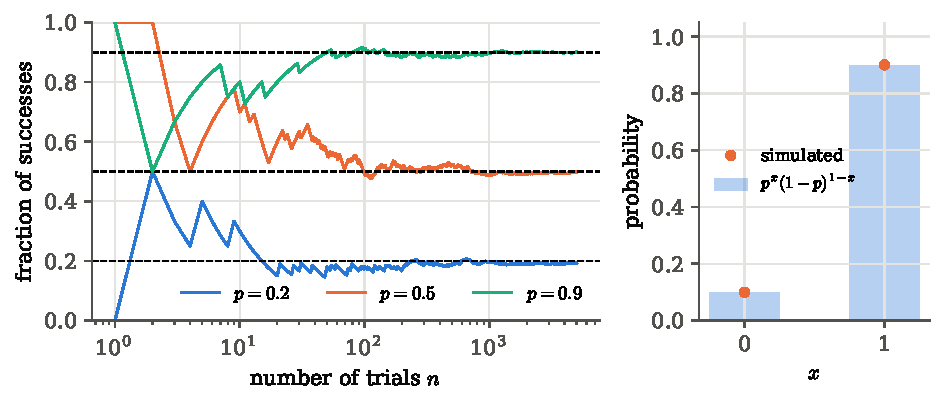
\includegraphics[width=\linewidth]{figures/ch02/01_bernoulli.pdf}
\caption{Left: the fraction of successes after $n$ trials, for three paddles. Early on the fraction jumps around wildly; by a few thousand trials each curve has settled onto its dashed line at $p$. Right: for $p=0.9$ the bars are the pmf and the dots the frequencies in a million simulated trials; they coincide.}
\label{2a:fig:bern-sim}
\end{figure}

For $10^6$ trials at $p=\twoaBernP$ the sample mean is $\twoaBernMean$ and the sample variance is $\twoaBernVar$, against the derived $p=\twoaBernP$ and $p(1-p)=\twoaBernVarTheory$ (\cref{2a:fig:bern-sim}). On the left, the running fraction slowly settles onto $p$: this is the law of large numbers at work. Its typical distance from $p$ after $n$ trials shrinks like $\sqrt{p(1-p)/n}$, which follows from the binomial variance in the next section.

\paragraph{What this bought us.}
A yes/no trial is fully described by one number $p$. The pmf $p^x(1-p)^{1-x}$ is built so that products over many independent trials collapse onto the number of successes. The mean is $p$ and the variance is $p(1-p)$, largest for a fair coin.

\section{Many successive trials: the binomial distribution}\label{2a:sec:binomial}

A cosmic-ray telescope is a stack of four scintillator layers. A muon going straight down crosses all four. Each layer fires independently with efficiency $\epsilon=0.95$, the probability that it fires when a muon crosses it. To reject noise, the trigger demands that \emph{at least three} of the four layers fire. What fraction of real muons does the trigger keep? Requiring all four would be cleaner, but how many muons would it cost? Both questions need the same thing: the probability of exactly $k$ successes in $n$ independent trials. The binomial distribution supplies it. It turns ``each trial succeeds with probability $p$'' into the full distribution of the number of successes.

\paragraph{Physical picture: paths through a tree.}
Picture each trial as a fork in a road: up for success, down for failure. After $n$ forks, every possible history is a path, and the number of successes is the number of ``up'' steps along that path. A random walk in one dimension has the same combinatorics. So do $n$ non-interacting spin-$\tfrac12$ particles: the number of spin-up particles is binomially distributed. The binomial coefficient $\binom nk$ that appears below is the \emph{multiplicity} of the macrostate ``$k$ up'', the same multiplicity that statistical mechanics uses to define entropy.

\paragraph{The question, step by step.}
\begin{enumerate}[leftmargin=1.6em,itemsep=1pt]
  \item What is the probability of one \emph{particular} sequence of outcomes, say success, failure, success? Multiply, because the trials are independent.
  \item Does that probability depend on the order? No: only on how many successes there are.
  \item How many sequences have exactly $k$ successes? Count them.
  \item So the probability of $k$ successes is (number of sequences) $\times$ (probability of each one).
\end{enumerate}

\begin{figure}[htbp]
\centering
\begin{tikzpicture}[
  st/.style={circle,draw=accent,fill=ideabg,inner sep=1.2pt,minimum size=5mm,font=\scriptsize},
  lf/.style={font=\scriptsize,anchor=west},
  up/.style={thick,formblue},
  dn/.style={thick,softgray}]
  \node[st] (r) at (0,0) {};
  \node[st] (s) at (2,1.6) {S};
  \node[st] (f) at (2,-1.6) {F};
  \draw[up] (r) -- (s); \draw[dn] (r) -- (f);
  \node[st] (ss) at (4,2.4) {S}; \node[st] (sf) at (4,0.8) {F};
  \node[st] (fs) at (4,-0.8) {S}; \node[st] (ff) at (4,-2.4) {F};
  \draw[up] (s) -- (ss); \draw[dn] (s) -- (sf);
  \draw[up] (f) -- (fs); \draw[dn] (f) -- (ff);
  \foreach \pa/\y/\name in {ss/2.8/sss, sf/1.2/sfs, fs/-0.4/fss, ff/-2.0/ffs}{
    \node[st] (\name) at (6,\y) {S}; \draw[up] (\pa) -- (\name);}
  \foreach \pa/\y/\name in {ss/2.0/ssf, sf/0.4/sff, fs/-1.2/fsf, ff/-2.8/fff}{
    \node[st] (\name) at (6,\y) {F}; \draw[dn] (\pa) -- (\name);}
  \node[lf] at (6.4,2.8)  {SSS \quad $k=3$\quad $p^3$};
  \node[lf] at (6.4,2.0)  {SSF \quad $k=2$\quad $p^2(1-p)$};
  \node[lf] at (6.4,1.2)  {SFS \quad $k=2$\quad $p^2(1-p)$};
  \node[lf] at (6.4,0.4)  {SFF \quad $k=1$\quad $p(1-p)^2$};
  \node[lf] at (6.4,-0.4) {FSS \quad $k=2$\quad $p^2(1-p)$};
  \node[lf] at (6.4,-1.2) {FSF \quad $k=1$\quad $p(1-p)^2$};
  \node[lf] at (6.4,-2.0) {FFS \quad $k=1$\quad $p(1-p)^2$};
  \node[lf] at (6.4,-2.8) {FFF \quad $k=0$\quad $(1-p)^3$};
  \node[font=\scriptsize,softgray] at (2,-3.4) {trial 1};
  \node[font=\scriptsize,softgray] at (4,-3.4) {trial 2};
  \node[font=\scriptsize,softgray] at (6,-3.4) {trial 3};
\end{tikzpicture}
\caption{All $2^3=8$ histories of three trials. Blue branches are successes (probability $p$), grey ones failures (probability $1-p$). Each path's probability is the product along it and depends only on its number of successes $k$. Counting paths per $k$ gives $1,3,3,1$, the third row of Pascal's triangle.}
\label{2a:fig:tree}
\end{figure}

\subsection{Deriving the pmf by counting paths}

Take $n$ independent trials, each a Bernoulli$(p)$. A history is a string of $n$ letters, S (success) or F (failure). By the product formula for independent Bernoulli trials (\cref{2a:sec:bernoulli}), a string with $k$ S's has probability $p^k(1-p)^{n-k}$ whatever the order.

\emph{How many strings have exactly $k$ S's?} We must choose which $k$ of the $n$ positions carry an S. Count ordered choices first: there are $n$ ways to pick the first position, $n-1$ for the second, and so on down to $n-k+1$ for the $k$-th, giving $n(n-1)\cdots(n-k+1)=\frac{n!}{(n-k)!}$ ordered choices. Each set of $k$ positions has been counted $k!$ times, once for each order in which we could have picked the same positions. So the number of sets is
\begin{equation}
  \binom nk \;=\; \frac{n!}{k!\,(n-k)!}, \label{2a:eq:binomcoef}
\end{equation}
the \newterm{binomial coefficient}, read ``$n$ choose $k$''. (By convention $0!=1$, so $\binom n0=\binom nn=1$.)

\begin{workdef}[binomial distribution]
$X\sim\mathrm{Binomial}(n,p)$ if $X$ is the number of successes in $n$ independent trials, each succeeding with the same probability $p$ \unpack{$n$ fixed in advance, trials do not influence each other, $p$ the same for every trial}. Its pmf is
\begin{equation}
  f(k\given n,p)\;=\;\binom nk\,p^k(1-p)^{n-k},\qquad k=0,1,\dots,n. \label{2a:eq:binom}
\end{equation}
\emph{Recognise it by:} multiple successive trials (where Bernoulli is for a single trial), a fixed number of them, each yes/no, independent, with constant $p$, and we record only the total number of successes.
\end{workdef}

\paragraph{It is normalised.} The probabilities \eqref{2a:eq:binom} add up to one. The tool is the \newterm{binomial theorem}: $(a+b)^n=\sum_{k=0}^n\binom nk a^kb^{n-k}$. Here is why it is true. Expanding the product of $n$ factors $(a+b)(a+b)\cdots(a+b)$ means choosing $a$ or $b$ from each factor. A term $a^kb^{n-k}$ arises once for each way of choosing which $k$ factors give $a$, and there are $\binom nk$ such ways. Then
\begin{align*}
  \sum_{k=0}^n f(k\given n,p) \eqby{1} \sum_{k=0}^n\binom nk p^k(1-p)^{n-k} \eqby{2} \bigl(p+(1-p)\bigr)^n = 1^n = 1 .
\end{align*}
\begin{explain}
  \item Definition \eqref{2a:eq:binom}.
  \item The binomial theorem with $a=p$ and $b=1-p$.
\end{explain}
With $p=\tfrac12$ the same line says $\sum_k\binom nk=2^n$: the total number of paths in the tree \srcref{CasellaBerger}{(3.2.4), p.~74}.

\subsection{Mean and variance, two ways}

\paragraph{The slick way: a sum of indicators.} Let $X_i$ be the indicator of success on trial $i$: it is $1$ if trial $i$ succeeds and $0$ otherwise. Counting successes is adding up these indicators, so $X=X_1+\dots+X_n$, and the $X_i$ are independent Bernoulli$(p)$.
\begin{align}
  \E X &\eqby{1} \sum_{i=1}^n\E X_i \eqby{2} np, \nonumber\\
  \Var X &\eqby{3} \sum_{i=1}^n\Var X_i \eqby{4} np(1-p). \label{2a:eq:binvar}
\end{align}
\begin{explain}
  \item Expectation is linear: $\E(\sum X_i)=\sum\E X_i$, with or without independence (\cref{ch:01}).
  \item $\E X_i=p$ from \eqref{2a:eq:bernvar}.
  \item For \emph{independent} variables the covariances vanish, so the variance of a sum is the sum of variances.
  \item $\Var X_i=p(1-p)$ from \eqref{2a:eq:bernvar}.
\end{explain}

\paragraph{The direct way: sum the pmf.} This route uses a trick that recurs throughout the chapter: absorb the factor $k$ into the binomial coefficient, then recognise the sum that is left as the total probability of a smaller distribution. The identity we need is
\[
  k\binom nk = k\frac{n!}{k!(n-k)!} = \frac{n!}{(k-1)!(n-k)!} = n\binom{n-1}{k-1}\qquad (k\ge1).
\]
Then
\begin{align*}
  \E X &\eqby{1} \sum_{k=1}^n k\binom nk p^k(1-p)^{n-k}
   \eqby{2} np\sum_{k=1}^n\binom{n-1}{k-1}p^{k-1}(1-p)^{(n-1)-(k-1)}\\
  &\eqby{3} np\sum_{j=0}^{n-1}\binom{n-1}{j}p^{j}(1-p)^{n-1-j}
   \eqby{4} np .
\end{align*}
\begin{explain}
  \item Definition of the mean. The $k=0$ term is zero, so we start at $k=1$.
  \item The identity above, and one factor $p$ taken out of $p^k$.
  \item Rename $j=k-1$.
  \item The sum is the total probability of a Binomial$(n-1,p)$, which is $1$.
\end{explain}
For the variance, the same trick works on the \emph{factorial moment} $\E[X(X-1)]$, using $k(k-1)\binom nk=n(n-1)\binom{n-2}{k-2}$:
\begin{align*}
  \E[X(X-1)] &\eqby{1} n(n-1)p^2\sum_{j=0}^{n-2}\binom{n-2}{j}p^j(1-p)^{n-2-j} \eqby{2} n(n-1)p^2,\\
  \Var X &\eqby{3} \E[X(X-1)]+\E X-(\E X)^2 = n(n-1)p^2+np-n^2p^2 = np(1-p).
\end{align*}
\begin{explain}
  \item The same three steps as for the mean, with two factors of $k$ absorbed and $j=k-2$.
  \item A Binomial$(n-2,p)$ sums to one.
  \item $\E X^2=\E[X(X-1)]+\E X$, and then the variance shortcut.
\end{explain}
Both ways agree with \srcref{Cowan}{(2.3)--(2.4), p.~27}.\footnote{Cowan writes the upper limit of the sum in (2.3) as $\infty$. It should be $n$, the number of trials, since the count cannot exceed it.}

\paragraph{What the numbers mean.} The mean count $np$ grows like $n$, but the standard deviation $\sqrt{np(1-p)}$ grows only like $\sqrt n$. Dividing both by $n$, the \emph{fraction} of successes $X/n$ has mean $p$ and standard deviation $\sqrt{p(1-p)/n}$. This is the rate at which the running fractions in \cref{2a:fig:bern-sim} settle, and the origin of every ``$1/\sqrt N$'' error bar on an efficiency.

\subsection{The moment generating function and sums of binomials}

The \newterm{moment generating function} (mgf) $M_X(t)=\E e^{tX}$ (\cref{ch:01}) packs all the moments into one function: its $r$-th derivative at $t=0$ is $\E X^r$. For the binomial,
\begin{align}
  M_X(t) \eqby{1} \sum_{k=0}^n e^{tk}\binom nk p^k(1-p)^{n-k}
  \eqby{2} \sum_{k=0}^n\binom nk (pe^t)^k(1-p)^{n-k}
  \eqby{3} \bigl(1-p+pe^t\bigr)^n . \label{2a:eq:binmgf}
\end{align}
\begin{explain}
  \item Definition of the mgf.
  \item $e^{tk}p^k=(pe^t)^k$.
  \item The binomial theorem with $a=pe^t$ and $b=1-p$.
\end{explain}
Check: $M'(0)=n(1-p+p)^{n-1}p=np$, the mean again.

\begin{keyidea}[binomials with the same $p$ add]
If $X_1\sim\mathrm{Binomial}(n_1,p)$ and $X_2\sim\mathrm{Binomial}(n_2,p)$ are independent, then $X_1+X_2\sim\mathrm{Binomial}(n_1+n_2,p)$.
\end{keyidea}
\emph{Why:} the counting story gives it at once. $X_1$ counts successes in $n_1$ trials, and $X_2$ counts them in another $n_2$ independent trials with the same $p$. So $X_1+X_2$ counts successes in $n_1+n_2$ such trials. The mgf says the same. The mgf of a sum of independent variables is the product of their mgfs, and $(1-p+pe^t)^{n_1}(1-p+pe^t)^{n_2}=(1-p+pe^t)^{n_1+n_2}$, the mgf \eqref{2a:eq:binmgf} of Binomial$(n_1+n_2,p)$. The same $p$ is essential: with different $p$'s the product is not of binomial form.

\subsection{Worked examples}

\paragraph{Example: the coincidence trigger.}
Return to the four-layer telescope from the start of the section. Each layer fires with $\epsilon=0.95$, independently, so the number of layers that fire is $X\sim\mathrm{Binomial}(4,0.95)$. The trigger needs $X\ge3$.
\begin{align*}
  \Prob(X\ge3) &\eqby{1} \binom43\epsilon^3(1-\epsilon)+\binom44\epsilon^4 \\
  &\eqby{2} 4(0.857375)(0.05)+0.81450625 \\
  &= 0.171475+0.814506 = 0.98598 .
\end{align*}
\begin{explain}
  \item Only $k=3$ and $k=4$ satisfy the condition. Add their pmf values.
  \item $0.95^3=0.857375$ and $0.95^4=0.81450625$.
\end{explain}
The 3-out-of-4 trigger keeps $98.6\%$ of muons. Demanding all four keeps only $\epsilon^4=\twoaTrigFour$, so the cleaner trigger loses about one muon in five. The simulation in \pyname{02_binomial.py} (one million four-layer events) gives $\twoaTrigSim$ against the exact $\twoaTrigExact$.

\paragraph{Example: the Chevalier de M\'er\'e's two bets.}
Is it more likely to get at least one six in $4$ rolls of a die, or at least one double six in $24$ rolls of two dice? The number of successes is binomial in both cases, and ``at least one'' is the complement of ``none'':
\begin{align*}
  \Prob(\text{at least one six in }4) &\eqby{1} 1-\binom40\Bigl(\tfrac16\Bigr)^0\Bigl(\tfrac56\Bigr)^4 = 1-0.4823 = 0.518,\\
  \Prob(\text{at least one double six in }24) &\eqby{2} 1-\Bigl(\tfrac{35}{36}\Bigr)^{24} = 1-0.5086 = 0.491 .
\end{align*}
\begin{explain}
  \item Binomial$(4,1/6)$ at $k=0$.
  \item Binomial$(24,1/36)$ at $k=0$: two dice show a double six with probability $1/36$.
\end{explain}
The gambler's intuition ($4\times\tfrac16=24\times\tfrac1{36}=\tfrac23$) is wrong because it adds probabilities of events that are not mutually exclusive \srcref{CasellaBerger}{Ex.~3.2.3, p.~75}. The same mistake appears in ``the probability of at least one fake signal in $N$ search bins is $N$ times the single-bin probability'': true only while that product is small (the look-elsewhere effect, \cref{ch:04}).

\paragraph{Example: drawing without replacement: the hypergeometric.}
The binomial needs the same $p$ on every trial. That fails when we sample \emph{without replacement} from a small population, because each draw changes what is left. A batch of $N=25$ front-end chips contains $M$ faulty ones. We test $K=10$ chips at random and find none faulty. How surprising is this if $M=6$?

The number of faulty chips in the sample follows the \newterm{hypergeometric} distribution. Count equally likely samples: there are $\binom NK$ ways to choose $K$ chips, and $\binom Mx\binom{N-M}{K-x}$ of them contain exactly $x$ faulty ones (choose $x$ of the $M$ faulty and $K-x$ of the $N-M$ good ones). So
\[
  \Prob(X=x\given N,M,K)=\frac{\binom Mx\binom{N-M}{K-x}}{\binom NK},
\]
with mean $KM/N$ and variance $\frac{KM}{N}\frac{(N-M)(N-K)}{N(N-1)}$. For our batch,
\begin{align*}
  \Prob(X=0) \eqby{1} \frac{\binom60\binom{19}{10}}{\binom{25}{10}} \eqby{2} \frac{92378}{3268760} = 0.028 .
\end{align*}
\begin{explain}
  \item Hypergeometric with $N=25$, $M=6$, $K=10$, $x=0$.
  \item $\binom{19}{10}=92378$ and $\binom{25}{10}=3268760$.
\end{explain}
If six chips were faulty, a clean sample is unlikely: under $3\%$ \srcref{CasellaBerger}{Ex.~3.2.1, p.~73}. The binomial with $p=M/N=0.24$ would give $(0.76)^{10}=0.064$, more than twice as large. Why the difference? Without replacement, each good chip drawn leaves a remaining pool that is \emph{more} faulty, so a clean run is rarer. The factor $(N-K)/(N-1)$ in the variance is the ``finite-population correction''. When the batch is much larger than the sample, $N\gg K$, this factor goes to one and the hypergeometric becomes the binomial.

\subsection{Python: repeat the $n$ trials, histogram the count}

The script \pyname{code/ch02/02_binomial.py} simulates the generating process itself, not the formula. It builds a table of uniform numbers, one row per experiment and one column per trial.

\pyfile[firstline=21,lastline=24,firstnumber=21]{code/ch02/02_binomial.py}{Binomial counts by running the trials}

\pyname{rng.uniform(size=(reps, n)) <= p} is a \pyname{reps}$\times n$ table of Bernoulli trials, built exactly as in \cref{2a:sec:bernoulli}. Summing along a row (\pyname{axis=1}) counts the successes in one experiment. The script does this $20\,000$ times for six $(n,p)$ pairs and overlays \pyname{scipy.stats.binom.pmf} as black ticks (\cref{2a:fig:binom-sim}).

\begin{figure}[htbp]
\centering
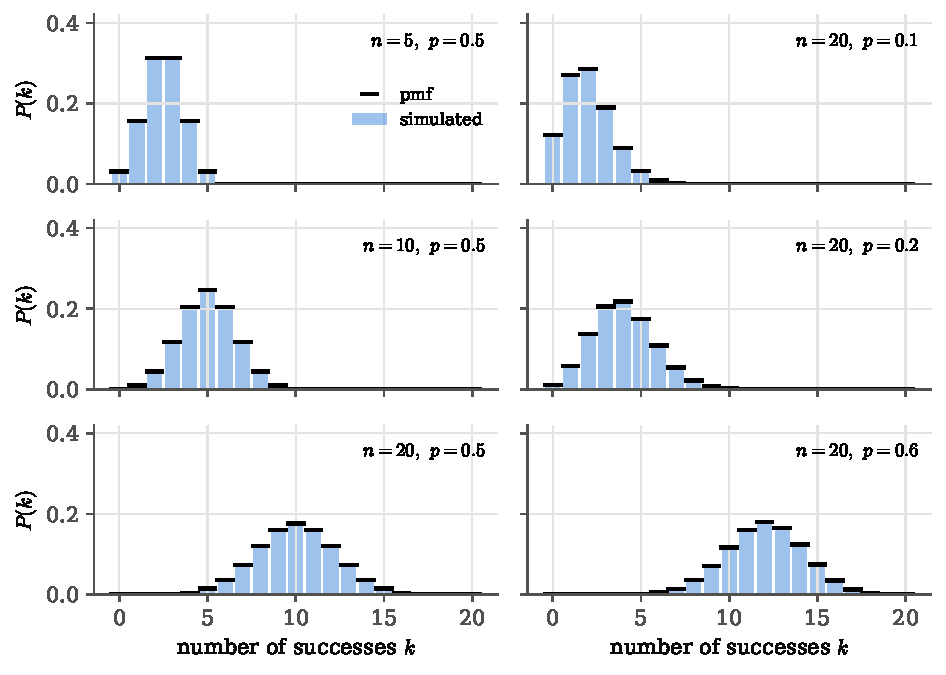
\includegraphics[width=0.95\linewidth]{figures/ch02/02_binomial.pdf}
\caption{Histograms of simulated success counts (bars) against the pmf (black ticks). Left column: $p=\tfrac12$ and more trials; the distribution stays symmetric, moves right and widens like $\sqrt n$. Right column: $n=20$ and growing $p$; at small $p$ the distribution is squashed against $k=0$ and skewed, at $p=0.6$ it leans the other way.}
\label{2a:fig:binom-sim}
\end{figure}

For $n=20$, $p=0.2$ and $200\,000$ experiments the sample mean is $\twoaBinMean$ and the sample variance $\twoaBinVar$, against $np=4$ and $np(1-p)=3.2$. \Cref{2a:fig:binom-sim} shows two features that matter later. For $p=\tfrac12$ and growing $n$ the shape is already bell-like: this is the de Moivre--Laplace limit, derived in the next part. For small $p$ the distribution piles up near zero with a tail to the right: this is the regime that becomes the Poisson distribution in \cref{2a:sec:poisson-limit}.

\begin{pitfall}[when the binomial is the wrong model]
Three assumptions go into \eqref{2a:eq:binom}, and each can fail in a real detector.
\begin{itemize}[leftmargin=1.4em,itemsep=1pt]
  \item \emph{Fixed $n$.} If the number of trials is itself random (the number of muons in a run), the count of successes is not binomial. We return to this in \cref{2a:sec:poisson-process}.
  \item \emph{Independence.} Layers that share a high-voltage supply fail together, so the number of dead layers is spread wider than binomial.
  \item \emph{Constant $p$.} Efficiency that varies across the paddle (edges versus centre), or between runs, also inflates the spread. The \emph{beta-binomial} distribution models a $p$ that itself varies \srcref{Lambert}{\S8.4.5}. Sampling without replacement (the hypergeometric example above) is the opposite case: the spread is \emph{narrower} than binomial.
\end{itemize}
A quick check is to compare the observed variance of a count with $np(1-p)$ computed from its observed mean.
\end{pitfall}

\section{Histogram bins: the multinomial distribution}\label{2a:sec:multinomial}

A calorimeter records the energy of $N=50$ electrons from a beta source, and we fill a histogram with $m=5$ energy bins. Each electron lands in bin $j$ with probability $p_j$, set by the shape of the spectrum. The number of electrons in bin $j$, the bin count $n_j$, fluctuates from one run to the next. To fit the spectrum later (\cref{ch:03}) we need the \emph{joint} distribution of all the bin contents, including how the bins fluctuate together. That joint distribution is the multinomial: the binomial with more than two outcomes. Its main lesson is that, with $N$ fixed, the bins of a histogram are \emph{negatively correlated}.

\paragraph{Physical picture: a fixed number of balls in boxes.}
Fifty balls are thrown one at a time into five boxes. If box 1 happens to catch more than its share, there are fewer balls left for the other boxes. The total is fixed, so the counts cannot all go up together. Statistical mechanics has the same situation in the canonical ensemble, where the particle number is fixed. Letting the total fluctuate, as in the grand canonical ensemble, removes the constraint. We will see that it also removes the correlation.

\paragraph{The question, step by step.}
\begin{enumerate}[leftmargin=1.6em,itemsep=1pt]
  \item What is the probability of one \emph{particular} sequence of bin assignments (electron 1 in bin 3, electron 2 in bin 1, \dots)? Multiply the $p$'s.
  \item Which feature of the sequence does that probability depend on? Only how many electrons went into each bin.
  \item How many sequences give the counts $(n_1,\dots,n_m)$? Count them.
  \item What does one bin look like on its own, and how do two bins co-vary?
\end{enumerate}

\subsection{Deriving the pmf}

Each of $N$ independent trials ends in one of $m$ outcomes, with probabilities $p_1,\dots,p_m$ and $\sum_jp_j=1$. A particular sequence with $n_1$ outcomes of type $1$, $n_2$ of type $2$, and so on, has probability $p_1^{n_1}p_2^{n_2}\cdots p_m^{n_m}$ by independence, whatever the order.

\emph{How many sequences have these counts?} Start by treating the $N$ trials as labelled objects in a row: there are $N!$ orderings. Many orderings give the same assignment of outcomes. Shuffling the $n_1$ trials of type $1$ among themselves ($n_1!$ ways) does not change which trials are of type $1$, and the same holds for every type. So each distinct assignment has been counted $n_1!\,n_2!\cdots n_m!$ times, and the number of distinct assignments is
\begin{equation}
  \binom{N}{n_1,n_2,\dots,n_m}\;=\;\frac{N!}{n_1!\,n_2!\cdots n_m!}, \label{2a:eq:multcoef}
\end{equation}
the \newterm{multinomial coefficient}. For $m=2$ it is $N!/(n_1!(N-n_1)!)$, the binomial coefficient.

\begin{workdef}[multinomial distribution]
The vector of counts $\bm n=(n_1,\dots,n_m)$ is $\mathrm{Multinomial}(N,\bm p)$ if it records how many of $N$ independent trials fell into each of $m$ categories, each trial landing in category $j$ with the same probability $p_j$ \unpack{$N$ fixed, categories exclusive and exhaustive, $\sum_jp_j=1$}. Its pmf is
\begin{equation}
  f(n_1,\dots,n_m\given N,\bm p)\;=\;\frac{N!}{n_1!\cdots n_m!}\,p_1^{n_1}\cdots p_m^{n_m},
  \qquad n_j\ge0,\quad \sum_jn_j=N. \label{2a:eq:mult}
\end{equation}
\emph{Recognise it by:} a histogram of a fixed number of independent entries, or any tally of categorical outcomes (particle species, decay channels, blood types).
\end{workdef}

The pmf \eqref{2a:eq:mult} sums to one by the \emph{multinomial theorem}, $(p_1+\dots+p_m)^N=\sum\frac{N!}{n_1!\cdots n_m!}p_1^{n_1}\cdots p_m^{n_m}$. It is proved exactly like the binomial theorem: expanding the product means picking one $p_j$ from each of the $N$ factors. The left side is $1^N=1$.

\begin{figure}[htbp]
\centering
\begin{tikzpicture}[x=10cm,y=1cm]
  \def\ca{0.4287}\def\cb{0.6887}\def\cc{0.8464}\def\cd{0.9420}
  \fill[formblue!45] (0,0) rectangle (\ca,0.4);
  \fill[formblue!32] (\ca,0) rectangle (\cb,0.4);
  \fill[formblue!22] (\cb,0) rectangle (\cc,0.4);
  \fill[formblue!14] (\cc,0) rectangle (\cd,0.4);
  \fill[formblue!7]  (\cd,0) rectangle (1,0.4);
  \draw[thick] (0,0) rectangle (1,0.4);
  \foreach \c in {\ca,\cb,\cc,\cd}{\draw[thick] (\c,0) -- (\c,0.4);}
  \node[font=\footnotesize] at (0.2143,0.2) {bin 1};
  \node[font=\footnotesize] at (0.5587,0.2) {bin 2};
  \node[font=\footnotesize] at (0.7675,0.2) {3};
  \node[font=\footnotesize] at (0.8942,0.2) {4};
  \node[font=\footnotesize] at (0.971,0.2) {5};
  \node[lbl,anchor=north] at (0,0) {$0$};
  \node[lbl,anchor=north] at (1,0) {$1$};
  \node[font=\scriptsize,anchor=north] at (\ca,0) {$p_1$};
  \node[font=\scriptsize,anchor=north] at (\cb,0) {$p_1{+}p_2$};
  \node[lbl,anchor=east] at (-0.02,0.2) {$u$};
  \fill[bdryred] (0.61,0.4) circle (1.2pt);
  \draw[->,thick,bdryred] (0.61,0.55) -- (0.61,0.43);
  \node[font=\scriptsize,bdryred,anchor=south] at (0.61,0.55) {$u=0.61$};
  \begin{scope}[yshift=-3.3cm]
    \foreach \j/\h in {1/2.14,2/1.30,3/0.79,4/0.48,5/0.29}{
      \draw[fill=formblue!30] ({(\j-1)*0.16+0.1},0) rectangle ({\j*0.16+0.1-0.02},\h);
      \node[font=\scriptsize,anchor=north] at ({(\j-0.5)*0.16+0.09},0) {$n_{\j}$};
    }
    \draw[faint] (0.08,0) -- (0.92,0);
    \node[font=\scriptsize,softgray,anchor=west] at (0.62,1.8) {expected counts $Np_j$};
  \end{scope}
\end{tikzpicture}
\caption{How one event chooses its bin. The unit interval is cut into pieces of lengths $p_1,\dots,p_5$ (a falling spectrum). A uniform number $u$ lands in one piece, here bin 2, and that bin's count goes up by one. Repeating this $N$ times fills the histogram below, whose bar heights are the expected counts $Np_j$ for $N=50$.}
\label{2a:fig:mult-bins}
\end{figure}

\subsection{One bin at a time: the marginal is binomial}

Often we care about one bin only. Then the other bins are \emph{nuisance} variables, and we \newterm{marginalise}: sum the joint pmf over all values of the variables we do not care about (\cref{ch:01}).

\begin{keyidea}[each bin is binomial]
If $\bm n\sim\mathrm{Multinomial}(N,\bm p)$, then $n_j\sim\mathrm{Binomial}(N,p_j)$ for every $j$.
\end{keyidea}
\emph{Why:} look at bin $j$ alone. Each trial either lands in bin $j$ (probability $p_j$) or does not (probability $1-p_j$). Lump all the other bins into the single outcome ``not in bin $j$'', and we have $N$ independent yes/no trials with the same probability: the binomial story. The algebra confirms it. Take three categories (bin $i$, bin $j$, ``everything else''), where the pmf is the \emph{trinomial}
\[
  f(n_i,n_j)=\frac{N!}{n_i!\,n_j!\,(N-n_i-n_j)!}\,p_i^{n_i}p_j^{n_j}(1-p_i-p_j)^{N-n_i-n_j}.
\]
Summing out $n_j$:
\begin{align*}
  \sum_{n_j=0}^{N-n_i} f(n_i,n_j)
  &\eqby{1} \frac{N!}{n_i!\,(N-n_i)!}p_i^{n_i}\sum_{n_j=0}^{N-n_i}\frac{(N-n_i)!}{n_j!\,(N-n_i-n_j)!}\,p_j^{n_j}(1-p_i-p_j)^{N-n_i-n_j}\\
  &\eqby{2} \binom N{n_i}p_i^{n_i}\,\bigl(p_j+1-p_i-p_j\bigr)^{N-n_i}
  \eqby{3} \binom N{n_i}p_i^{n_i}(1-p_i)^{N-n_i}.
\end{align*}
\begin{explain}
  \item Multiply and divide by $(N-n_i)!$, and take out everything that does not depend on $n_j$.
  \item The remaining sum is the binomial theorem with $n=N-n_i$, $a=p_j$, $b=1-p_i-p_j$.
  \item The two $p_j$'s cancel.
\end{explain}
The result is the Binomial$(N,p_i)$ pmf, so $\E n_i=Np_i$ and $\Var n_i=Np_i(1-p_i)$ from \eqref{2a:eq:binvar}, and the same holds for every bin. Summing over the nuisance bin removed it and left the distribution of the one bin we care about.

\subsection{Two bins together: the covariance}

The question is how two bin counts $n_i$ and $n_j$ fluctuate together. The tool is the same as for the binomial mean: write each count as a sum of indicators, one per event. Let $I_{e j}$ be the indicator that event $e$ landed in bin $j$ (it is $1$ if so, $0$ if not). Then $n_j=\sum_{e=1}^N I_{ej}$. Two facts about these indicators do all the work:
\begin{itemize}[leftmargin=1.4em,itemsep=1pt]
  \item \emph{same event, different bins:} one event lands in exactly one bin, so $I_{ei}I_{ej}=0$ for $i\ne j$;
  \item \emph{different events:} $I_{ei}$ and $I_{e'j}$ are independent for $e\ne e'$, so their covariance is zero.
\end{itemize}
For $i\neq j$,
\begin{align}
  \Cov(n_i,n_j)
  &\eqby{1} \sum_{e=1}^N\sum_{e'=1}^N \Cov(I_{ei},I_{e'j})
   \eqby{2} \sum_{e=1}^N \Cov(I_{ei},I_{ej}) \nonumber\\
  &\eqby{3} \sum_{e=1}^N\bigl(\E[I_{ei}I_{ej}]-\E I_{ei}\,\E I_{ej}\bigr)
   \eqby{4} \sum_{e=1}^N (0-p_ip_j) = -Np_ip_j . \label{2a:eq:multcov}
\end{align}
\begin{explain}
  \item Covariance is linear in each argument, so the covariance of two sums is the sum of all pairwise covariances.
  \item Terms with $e\ne e'$ vanish: different events are independent.
  \item Definition $\Cov(A,B)=\E[AB]-\E A\,\E B$.
  \item $I_{ei}I_{ej}=0$, and $\E I_{ej}=p_j$ because an indicator is Bernoulli.
\end{explain}
Together with the variances, the full \newterm{covariance matrix} of the histogram is
\begin{equation}
  \Cmat_{ij}\;=\;\Cov(n_i,n_j)\;=\;N\bigl(p_i\delta_{ij}-p_ip_j\bigr),
  \qquad \Cmat=N\bigl(\diag(\bm p)-\bm p\bm p\T\bigr), \label{2a:eq:multC}
\end{equation}
and the correlation of two bins is
\[
  \Corr(n_i,n_j)=\frac{-Np_ip_j}{\sqrt{Np_i(1-p_i)\,Np_j(1-p_j)}}=-\sqrt{\frac{p_ip_j}{(1-p_i)(1-p_j)}} .
\]
It does not depend on $N$: more events do not make the anti-correlation go away.

\paragraph{The matrix is singular.} Every row of $\Cmat$ sums to zero: $\sum_jN(p_i\delta_{ij}-p_ip_j)=N(p_i-p_i\sum_jp_j)=0$. So the vector $\bm 1=(1,\dots,1)$ is a zero mode, $\Cmat\,\bm 1=0$, and $\Var(\sum_jn_j)=\bm1\T\Cmat\bm1=0$. This is no surprise: the total $\sum_jn_j=N$ does not fluctuate at all. A $\chi^2$ built from the full $\Cmat$ must therefore drop one bin or use a pseudo-inverse, a point that returns when we fit histograms (\cref{ch:03}).

\subsection{Worked examples}

\paragraph{Example: a die rolled twelve times.}
What is the probability that a fair die rolled $12$ times shows each face exactly twice?
\begin{align*}
  f(2,2,2,2,2,2) \eqby{1} \frac{12!}{(2!)^6}\Bigl(\tfrac16\Bigr)^{12}
  \eqby{2} \frac{479001600}{64}\cdot\frac{1}{2176782336}
  = \frac{7484400}{2176782336} = 0.00344 .
\end{align*}
\begin{explain}
  \item Multinomial with $N=12$, $m=6$, all $p_j=1/6$, all $n_j=2$.
  \item $12!=479001600$, $(2!)^6=64$ and $6^{12}=2176782336$.
\end{explain}
The ``perfectly flat'' histogram is rare: about one run in $290$. A histogram that looks too flat should make us as suspicious as one that looks too bumpy.

\paragraph{Example: blood groups in a sample.}
In a population the ABO blood groups O, A, B, AB have frequencies roughly $p=(0.45,0.40,0.11,0.04)$. In a sample of $N=10$ donors, what is the probability of exactly $5$ O, $4$ A, $1$ B and no AB?
\begin{align*}
  f \eqby{1} \frac{10!}{5!\,4!\,1!\,0!}\,(0.45)^5(0.40)^4(0.11)^1(0.04)^0
  \eqby{2} 1260\times0.018453\times0.0256\times0.11 = 0.0655 .
\end{align*}
\begin{explain}
  \item Multinomial pmf with $N=10$, $m=4$.
  \item $10!/(5!\,4!)=3628800/(120\times24)=1260$, $0.45^5=0.018453$, $0.40^4=0.0256$.
\end{explain}
Each donor is one categorical trial. The multinomial aggregates the categorical outcomes into counts \srcref{Lambert}{\S8.4.10}, exactly as a histogram aggregates individual events into bins.

\paragraph{Example: the covariance of the first two bins of the spectrum.}
Return to the beta spectrum from the start of the section: $N=50$ electrons in five bins. Take a falling spectrum, with the five bin probabilities proportional to $e^{-j/2}$ for $j=0,\dots,4$. Normalising them to sum to one gives $p_1=\twoaMultPone$ and $p_2=\twoaMultPtwo$ for the first two bins. Then
\begin{align*}
  \Var n_1 &= Np_1(1-p_1) = 50\times0.4287\times0.5713 = 12.25,\\
  \Cov(n_1,n_2) &= -Np_1p_2 = -50\times0.4287\times0.2600 = -5.57,\\
  \Corr(n_1,n_2) &= -\sqrt{\frac{0.4287\times0.2600}{0.5713\times0.7400}} = -0.513 .
\end{align*}
A strong anti-correlation: a run with an excess in the first bin very probably has a deficit in the second.

\subsection{Python: drop the events into the bins}

\pyfile[firstline=20,lastline=32,firstnumber=20]{code/ch02/03_multinomial.py}{Filling many histograms event by event}

The function \pyname{histogram_of_events} is \cref{2a:fig:mult-bins} in code. \pyname{np.cumsum(p)} gives the cut points $p_1,\,p_1+p_2,\dots$ of the unit interval; \pyname{np.searchsorted} returns, for each uniform number, the index of the piece it fell into, that is, the bin; \pyname{np.bincount} counts the events per bin. Line 31 fills $30\,000$ histograms with exactly $N=50$ events. Line 32 does the same but first draws the number of events from a Poisson distribution with mean $50$ (the distribution of \cref{2a:sec:poisson-limit}), to see what happens when the total is allowed to fluctuate.

\begin{figure}[htbp]
\centering
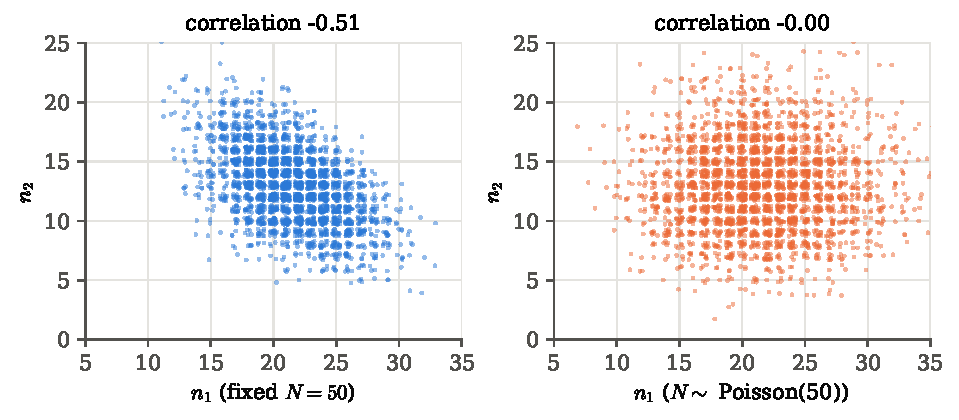
\includegraphics[width=\linewidth]{figures/ch02/03_multinomial.pdf}
\caption{Contents of bin 2 against bin 1 for $3000$ simulated histograms (a small random jitter separates the integer points). Left: with exactly $50$ events per histogram the cloud slopes downwards, because an extra event in bin 1 is an event missing from somewhere else. Right: when the number of events is itself Poisson, the cloud is round and the two bins are uncorrelated.}
\label{2a:fig:mult-sim}
\end{figure}

The simulated variance of bin 1 is $\twoaMultVarOneSim$ (theory $\twoaMultVarOneTh$), the covariance of bins 1 and 2 is $\twoaMultCovSim$ (theory $\twoaMultCovTh$) and their correlation is $\twoaMultCorrSim$ (theory $\twoaMultCorrTh$). The variance of the row sums is exactly $\twoaMultRowSumVar$: the zero mode of $\Cmat$. With a Poisson number of events the correlation drops to $\twoaMultCorrPois$, compatible with zero (\cref{2a:fig:mult-sim}). We prove in \cref{2a:sec:poisson-process} that Poisson-distributed totals make the bins \emph{exactly} independent. This is why fits to histograms whose total is not fixed in advance (most collider analyses) may treat bins as independent Poisson counts.

\begin{pitfall}[independent bins are an assumption]
It is tempting to treat histogram bins as independent, each with error $\sqrt{n_j}$. With a fixed number of entries that is wrong: the bins are anti-correlated by \eqref{2a:eq:multcov}. For many bins with small $p_j$ the correlation $\approx-\sqrt{p_ip_j}$ is small and the independent approximation is usually fine; for a histogram with a few dominant bins it is not. Normalised shapes (``unit-area'' histograms) always carry this constraint.
\end{pitfall}

\section{Rare events in many trials: the Poisson distribution}\label{2a:sec:poisson-limit}

A microgram of a long-lived isotope contains of order $10^{15}$ nuclei. In one second each nucleus decays with a tiny probability $p$, and the decays are independent. A Geiger counter records the number of decays in each one-second window. Strictly, this count is Binomial$(n,p)$ with $n\approx10^{15}$ nuclei. But nobody knows $n$ or $p$ separately, and nobody wants to evaluate $\binom{10^{15}}{k}$. What we \emph{can} measure is the average number of clicks per window, $\lambda=np$. The Poisson distribution is what the binomial becomes when the trials are very many, each is very unlikely to succeed, and only their product $\lambda$ matters. It is the distribution of \emph{counts of rare events}.

\paragraph{Physical picture: rare, independent, many.}
Photons arriving at a CCD pixel, dark counts in a photomultiplier, cosmic rays through a detector, events in one bin of a collider histogram, galaxies in a small cell of a sparse survey: each count is the sum of a huge number of chances, each tiny, none influencing the others. In every one of these cases only the mean count $\lambda$ enters the answer. The microscopic details, such as how many photons were emitted upstream or how many protons collided, drop out.

\paragraph{The question, step by step.}
\begin{enumerate}[leftmargin=1.6em,itemsep=1pt]
  \item Start from the exact binomial for $n$ trials with $p=\lambda/n$, so that the mean $np=\lambda$ stays fixed.
  \item Let $n\to\infty$. Which factors change and which survive?
  \item Is the limit a proper distribution? What are its mean and variance?
  \item How large must $n$ be for the approximation to be good?
\end{enumerate}

\subsection{The limit, line by line}

The derivation needs one limit from calculus. We prove it first.

\paragraph{The compound-interest limit.} For any fixed real $\lambda$, $\displaystyle\lim_{n\to\infty}\Bigl(1-\frac\lambda n\Bigr)^n=e^{-\lambda}$.
\emph{Why:} take the logarithm and use the Taylor series $\ln(1-x)=-x-\tfrac{x^2}2-\tfrac{x^3}3-\cdots$, valid for $\abs x<1$:
\begin{align*}
  \ln\Bigl(1-\frac\lambda n\Bigr)^n
  \eqby{1} n\ln\Bigl(1-\frac\lambda n\Bigr)
  \eqby{2} n\Bigl(-\frac\lambda n-\frac{\lambda^2}{2n^2}-\cdots\Bigr)
  = -\lambda-\frac{\lambda^2}{2n}-\cdots
  \;\xrightarrow{\;n\to\infty\;}\; -\lambda .
\end{align*}
\begin{explain}
  \item $\ln a^n=n\ln a$.
  \item Taylor series with $x=\lambda/n$, which is less than one in size once $n>\abs\lambda$.
\end{explain}
Exponentiate: the limit is $e^{-\lambda}$. \Cref{2a:fig:compound} shows how fast it is approached. The correction $-\lambda^2/(2n)$ in the exponent tells us that $(1-\lambda/n)^n$ is always a little \emph{below} $e^{-\lambda}$, by a relative amount of about $\lambda^2/2n$.

\begin{figure}[htbp]
\centering
\begin{tikzpicture}
\begin{axis}[width=10cm,height=5.2cm,xmin=0,xmax=62,ymin=0,ymax=0.056,
  xlabel={number of trials $n$},ylabel={$(1-3/n)^n$},
  ytick={0,0.01,0.02,0.03,0.04,0.05},yticklabel style={/pgf/number format/fixed,/pgf/number format/precision=2},
  axis lines=left,tick label style={font=\scriptsize},label style={font=\small}]
  \addplot[only marks,mark=*,mark size=1.3pt,formblue,samples at={4,5,...,60}] {(1-3/x)^x};
  \addplot[dashed,black,domain=0:62] {exp(-3)};
  \node[font=\scriptsize,anchor=south east] at (axis cs:60,0.0505) {$e^{-3}=0.0498$};
\end{axis}
\end{tikzpicture}
\caption{The probability that none of $n$ nuclei decays, when each decays with probability $3/n$. With four nuclei it is tiny; as the nuclei become more numerous and individually less likely to decay, it climbs towards the dashed limit $e^{-3}$, getting within ten per cent of it by $n\approx50$.}
\label{2a:fig:compound}
\end{figure}

With this limit in hand, we can take the binomial to the Poisson. Put $p=\lambda/n$ into the binomial pmf \eqref{2a:eq:binom}, so that the mean $np=\lambda$ stays fixed, and hold the count $k$ fixed while $n$ grows:
\begin{align}
  \binom nk p^k(1-p)^{n-k}
  &\eqby{1} \frac{n!}{k!\,(n-k)!}\,\frac{\lambda^k}{n^k}\Bigl(1-\frac\lambda n\Bigr)^{n}\Bigl(1-\frac\lambda n\Bigr)^{-k} \nonumber\\
  &\eqby{2} \frac{\lambda^k}{k!}\;\cdot\;\frac{n(n-1)\cdots(n-k+1)}{n^k}\;\cdot\;\Bigl(1-\frac\lambda n\Bigr)^{n}\;\cdot\;\Bigl(1-\frac\lambda n\Bigr)^{-k} \nonumber\\
  &\eqby{3} \frac{\lambda^k}{k!}\;\cdot\;\Bigl(1-\frac1n\Bigr)\Bigl(1-\frac2n\Bigr)\cdots\Bigl(1-\frac{k-1}n\Bigr)\;\cdot\;\Bigl(1-\frac\lambda n\Bigr)^{n}\;\cdot\;\Bigl(1-\frac\lambda n\Bigr)^{-k} \nonumber\\
  &\xrightarrow{\;n\to\infty\;} \frac{\lambda^k}{k!}\cdot 1\cdot e^{-\lambda}\cdot 1 . \label{2a:eq:poislimit}
\end{align}
\begin{explain}
  \item Substitute $p=\lambda/n$ and split $(1-p)^{n-k}=(1-p)^n(1-p)^{-k}$.
  \item Regroup. $n!/(n-k)!=n(n-1)\cdots(n-k+1)$ has exactly $k$ factors.
  \item Divide each of the $k$ factors by one of the $k$ powers of $n$.
\end{explain}
Now take the four factors in the third line of the chain one at a time as $n\to\infty$. The first, $\lambda^k/k!$, does not involve $n$. In the second, each of the $k-1$ brackets $(1-j/n)$ goes to $1$; there is a \emph{fixed} number of them because $k$ is fixed, so their product goes to $1$. The third, $(1-\lambda/n)^n$, goes to $e^{-\lambda}$ by the compound-interest limit. The fourth is a fixed power, $-k$, of something that goes to one, so it goes to one.

\begin{workdef}[Poisson distribution]
$X\sim\mathrm{Poisson}(\lambda)$ if
\begin{equation}
  f(k\given\lambda)\;=\;e^{-\lambda}\,\frac{\lambda^k}{k!},\qquad k=0,1,2,\dots \label{2a:eq:pois}
\end{equation}
for some $\lambda>0$ \unpack{the mean number of events, a real number, not necessarily an integer}. There is no upper limit on $k$.
\emph{Recognise it by:} a count of events that are individually rare and mutually independent, out of a very large (or unknown) number of opportunities.
\end{workdef}

The number of trials $n$ has disappeared. The only parameter left is the mean count $\lambda$, the one thing we can measure.

\subsection{Normalisation, mean, variance, mgf}

Every sum here is the exponential series $e^{x}=\sum_{k=0}^\infty x^k/k!$, valid for every real (or complex) $x$, in disguise.
\begin{align*}
  \sum_{k=0}^\infty f(k) &\eqby{1} e^{-\lambda}\sum_{k=0}^\infty\frac{\lambda^k}{k!} \eqby{2} e^{-\lambda}e^{\lambda}=1,\\
  \E X &\eqby{3} e^{-\lambda}\sum_{k=1}^\infty k\frac{\lambda^k}{k!}
       \eqby{4} \lambda e^{-\lambda}\sum_{k=1}^\infty\frac{\lambda^{k-1}}{(k-1)!}
       \eqby{2} \lambda e^{-\lambda}e^{\lambda}=\lambda,\\
  \E[X(X-1)] &\eqby{5} e^{-\lambda}\sum_{k=2}^\infty k(k-1)\frac{\lambda^k}{k!}
       = \lambda^2 e^{-\lambda}\sum_{k=2}^\infty\frac{\lambda^{k-2}}{(k-2)!} \eqby{2} \lambda^2,\\
  \Var X &\eqby{6} \E[X(X-1)]+\E X-(\E X)^2 = \lambda^2+\lambda-\lambda^2=\lambda .
\end{align*}
\begin{explain}
  \item Take the constant $e^{-\lambda}$ out of the sum.
  \item Exponential series (after renaming $j=k-1$ or $j=k-2$).
  \item The $k=0$ term vanishes.
  \item $k/k!=1/(k-1)!$, and one factor $\lambda$ taken out.
  \item The same trick with $k(k-1)/k!=1/(k-2)!$; the $k=0,1$ terms vanish.
  \item As for the binomial.
\end{explain}
\begin{keyidea}[mean equals variance]
For a Poisson count, $\E X=\Var X=\lambda$. The standard deviation is $\sqrt\lambda$, and the \emph{relative} fluctuation is $1/\sqrt\lambda$.
\end{keyidea}
So a Poisson count has mean and variance both equal to $\lambda$. Its standard deviation is $\sqrt\lambda$, and its \emph{relative} fluctuation, standard deviation over mean, is $1/\sqrt\lambda$. This is the origin of the ``$\sqrt N$'' error bar on a count, and of photon shot noise: to measure a flux to $1\%$ we need $1/\sqrt\lambda=0.01$, that is, about $10^4$ photons. The same results follow from the binomial ones by taking the limit: $np=\lambda$ and $np(1-p)=\lambda(1-\lambda/n)\to\lambda$.

The mgf is
\begin{align}
  M_X(t) \eqby{1} e^{-\lambda}\sum_{k=0}^\infty\frac{(\lambda e^t)^k}{k!} \eqby{2} e^{-\lambda}e^{\lambda e^t}=\exp\bigl[\lambda(e^t-1)\bigr]. \label{2a:eq:poismgf}
\end{align}
\begin{explain}
  \item $e^{tk}\lambda^k=(\lambda e^t)^k$.
  \item Exponential series with $x=\lambda e^t$.
\end{explain}
It is also the limit of the binomial mgf: $(1+p(e^t-1))^n=(1+\lambda(e^t-1)/n)^n\to e^{\lambda(e^t-1)}$ by the same compound-interest limit.

\paragraph{The shape: a recursion.} Dividing consecutive terms of \eqref{2a:eq:pois},
\begin{equation}
  \frac{f(k)}{f(k-1)}=\frac{e^{-\lambda}\lambda^k/k!}{e^{-\lambda}\lambda^{k-1}/(k-1)!}=\frac\lambda k . \label{2a:eq:poisrec}
\end{equation}
Each step from $k-1$ to $k$ multiplies the probability by $\lambda/k$. That factor is larger than one while $k<\lambda$ and smaller than one once $k>\lambda$. So the pmf rises while $k<\lambda$ and falls once $k>\lambda$. The most probable count is $\lfloor\lambda\rfloor$ (and if $\lambda$ is an integer, $\lambda-1$ and $\lambda$ are equally probable). The recursion is also the numerically stable way to compute the pmf: start at $f(0)=e^{-\lambda}$ and multiply by $\lambda/k$, never forming $\lambda^k$ or $k!$ separately \srcref{CasellaBerger}{(3.2.6)--(3.2.7), p.~77}.

\subsection{How good is the approximation?}

A convenient single number for the distance between two distributions $f$ and $g$ on the integers is the \newterm{total variation distance} $\mathrm{TV}(f,g)=\tfrac12\sum_k\abs{f(k)-g(k)}$ \unpack{the largest possible difference between the probabilities the two distributions give to the same event}. For the binomial with $p=\lambda/n$ and the Poisson with the same mean, a classical inequality due to Le~Cam states
\[
  \mathrm{TV}\bigl(\mathrm{Binomial}(n,\lambda/n),\,\mathrm{Poisson}(\lambda)\bigr)\;\le\;np^2\;=\;\frac{\lambda^2}{n}.
\]
Why $np^2$? Each Bernoulli trial differs from a Poisson$(p)$ variable only in the rare event of two or more ``successes'' in one trial, which has probability of order $p^2$. There are $n$ trials, so the differences add up to at most about $np^2$. The script \pyname{code/ch02/04_poisson_limit.py} computes the actual distance for $\lambda=3$: $\twoaTVfive$ at $n=5$, $\twoaTVtwenty$ at $n=20$, $\twoaTVhundred$ at $n=100$ and $\twoaTVthousand$ at $n=1000$. It falls like $1/n$, as the bound says, but is about ten times smaller than the bound.

\subsection{Worked examples}

\paragraph{Example: a typesetter's errors, exact and Poisson.}
A typesetter makes on average one error per $500$ words. Five pages of $300$ words hold $1500$ words. What is the probability of at most two errors? Exactly, $X\sim\mathrm{Binomial}(1500,1/500)$; approximately, $X\sim\mathrm{Poisson}(3)$.
\begin{align*}
  \Prob(X\le2) &\approx e^{-3}\Bigl(1+3+\frac{3^2}{2}\Bigr) \eqby{1} 0.049787\times8.5 = 0.4232 .
\end{align*}
\begin{explain}
  \item Sum of \eqref{2a:eq:pois} for $k=0,1,2$ with $\lambda=np=1500/500=3$.
\end{explain}
The exact binomial gives $\twoaTypExact$; the Poisson approximation gives $\twoaTypPois$, wrong in the fourth decimal \srcref{CasellaBerger}{Ex.~3.2.5, p.~77}.

\paragraph{Example: photomultiplier dark counts.}
A photomultiplier produces on average $5$ dark pulses every $3$~ms. In the next $1$~ms, what is the probability of no dark pulse, and of at least two? The count in $1$~ms is Poisson with $\lambda=5/3$.
\begin{align*}
  \Prob(X=0) &= e^{-5/3} = 0.189,\\
  \Prob(X\ge2) &\eqby{1} 1-\Prob(X=0)-\Prob(X=1) \eqby{2} 1-0.189-\tfrac53(0.189) = 1-0.189-0.315 = 0.496 .
\end{align*}
\begin{explain}
  \item Complement of ``zero or one''.
  \item $\Prob(X=1)=\lambda e^{-\lambda}$, which is $\lambda$ times $\Prob(X=0)$ by the recursion \eqref{2a:eq:poisrec}.
\end{explain}
So a $1$~ms coincidence window contains at least two dark pulses half the time: at this rate, a two-fold coincidence of dark noise is not rare. The numbers are those of a telephone switchboard in \srcref{CasellaBerger}{Ex.~3.2.4, p.~76}, a reminder that the Poisson story does not care what is being counted.

\paragraph{Example: events in a collider signal region.}
A new process has cross-section $\sigma=0.5$~fb, the data set has integrated luminosity $L=20~\text{fb}^{-1}$ and the selection efficiency is $\epsilon=0.3$. Each of the enormous number of proton--proton collisions has a tiny, independent chance to produce a selected signal event, so the number of selected events is Poisson with mean \srcref{Cowan}{(2.12), p.~30}
\[
  \lambda=\sigma L\epsilon=0.5\times20\times0.3=3 .
\]
The chance of seeing \emph{nothing} is $f(0\given3)=e^{-3}=0.0498$, about $5\%$. Read backwards, this is the classic ``three events'' rule: if we see zero events, any model predicting $\lambda\ge3$ is excluded at about $95\%$ confidence (\cref{ch:04}).

\subsection{Python: literally many nuclei}

\pyfile[firstline=24,lastline=28,firstnumber=24]{code/ch02/04_poisson_limit.py}{Counting decays of 2000 nuclei per window}

Each counting window gets $2000$ fresh uniform numbers, one per nucleus, and a nucleus ``decays'' if its number is below $\lambda/n=3/2000$. The count per window is the number of decays. Nothing in this code mentions $e^{-\lambda}$ or $k!$: the Poisson law has to emerge from the process. The script then computes the total variation distances quoted above and the typesetter example.

\begin{figure}[htbp]
\centering
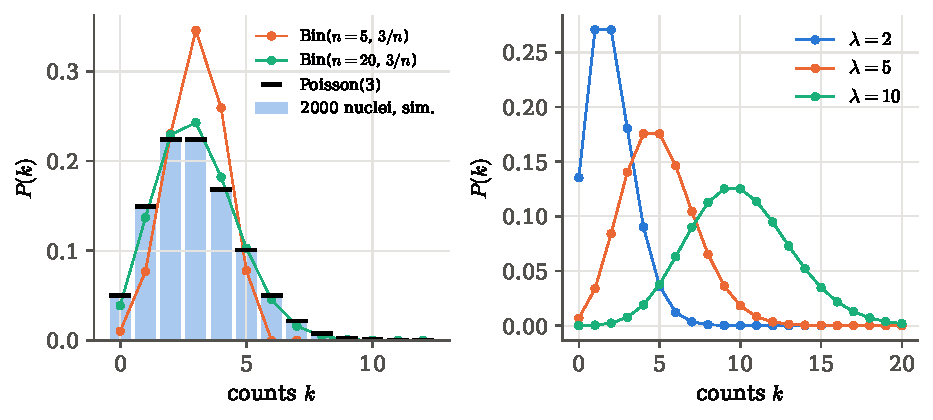
\includegraphics[width=\linewidth]{figures/ch02/04_poisson_limit.pdf}
\caption{Left: the histogram of decay counts from $2000$ simulated nuclei per window (bars) sits on the Poisson(3) pmf (black ticks). The binomials with only $5$ or $20$ trials and the same mean are visibly narrower, because each trial can produce at most one event. Right: Poisson shapes for $\lambda=2,5,10$; skewed to the right at small $\lambda$, nearly symmetric by $\lambda=10$.}
\label{2a:fig:pois-limit}
\end{figure}

Over $20\,000$ windows the sample mean is $\twoaPLMean$ and the sample variance is $\twoaPLVar$, equal within the statistical error as \emph{mean $=$ variance} demands. The fraction of empty windows is $\twoaPLZeroSim$, against $e^{-3}=\twoaPLZeroTh$ (\cref{2a:fig:pois-limit}). The right panel reproduces the shapes of \srcref{Cowan}{Fig.~2.3, p.~29}. The growing symmetry with $\lambda$ is the start of the Gaussian limit, previewed in \cref{2a:sec:failures}.

\paragraph{What this bought us.}
When many independent chances each have a small probability, the count is Poisson with the single parameter $\lambda=np$. Its variance equals its mean, so the relative scatter of a count is $1/\sqrt\lambda$. The approximation error is of order $\lambda^2/n$, negligible for any macroscopic number of trials.

\begin{pitfall}[``rare'' refers to each trial, not to the count]
The count itself need not be small: a CCD pixel may collect $10^5$ photons, and that count is still Poisson, because each of the $10^{20}$ photons emitted by the star had a tiny chance of landing in this pixel. What must be small is the probability per opportunity, and what must hold is independence. Conversely, a small count is not automatically Poisson: the number of dead channels in a $4$-channel module is binomial with $n=4$, and \cref{2a:fig:pois-limit} shows how different that can be.
\end{pitfall}

\section{The Poisson process: constant rate, no memory}\label{2a:sec:poisson-process}

In \cref{2a:sec:poisson-limit} the Poisson distribution came from a binomial over $n$ nuclei, each with a tiny chance to decay. Often there is no such $n$ to imagine. Cosmic rays arrive from the sky, photons from a distant quasar, dark pulses from a photocathode. All we know is that events come \emph{at random in time}, with some average rate $\lambda$ (events per second), and that the process has no memory: what happened in the last second does not affect the next. These two physical statements are enough. Through a differential equation, they force the count in any window of length $t$ to be Poisson$(\lambda t)$. The same machinery then shows that three common operations give Poisson counts again: thinning a Poisson stream (losing events at random), adding two streams, and splitting one into histogram bins.

\paragraph{Physical picture: a master equation with one-way hops.}
Think of the count $N(t)$, the number of events up to time $t$, as the state of a system that can only climb a ladder: $0\to1\to2\to\cdots$, one rung at a time, with hopping rate $\lambda$ from every rung. The probability of being on rung $n$ is fed from rung $n-1$ and drains into rung $n+1$. The rate equations for a radioactive decay chain have exactly this form, and so does the master equation of a birth process in statistical mechanics.

\paragraph{The question, step by step.}
\begin{enumerate}[leftmargin=1.6em,itemsep=1pt]
  \item What exactly do ``random in time at rate $\lambda$'' and ``no memory'' assume? State the inputs, then derive what they imply for a very short interval $h$.
  \item How does the probability of having $n$ events by time $t$ change between $t$ and $t+h$?
  \item Let $h\to0$ to get differential equations, and solve them.
  \item What happens to such a stream when we lose some events, add another stream, or sort the events into bins?
\end{enumerate}

\subsection{From three physical inputs to the short-interval rules}
\label{2a:sec:poisson-inputs}

Think of photons from a star whose brightness does not change. Even a perfect
detector does not count the same number in every exposure, because the photons
arrive one at a time at random instants. That scatter is \newterm{shot noise}.
It is not interference added to the signal. It is what counting discrete,
independent arrivals means. We now find its distribution from first principles:
we say exactly what we assume about the arrivals, and derive everything else.

\emph{The inputs.} Three are physical, and one is a mathematical regularity
condition.
\begin{enumerate}[label=(P\arabic*),leftmargin=2.6em,itemsep=1pt]
  \item \emph{No memory.} The numbers of events in non-overlapping time windows
        are independent. An arrival tells us nothing about when the next one comes.
  \item \emph{Constant rate.} The distribution of the count in a window depends
        only on its length, not on when it starts. The source does not brighten
        or fade during the exposure.
  \item \emph{One at a time.} Events arrive singly, never in bunches at the same
        instant.
  \item[(R)] \emph{Regularity.} The probability $P_0(h)$ that a window of length
        $h$ is empty changes continuously with $h$. This is a property we demand of
        the mathematics, not a statement about photons.
\end{enumerate}

\emph{The empty window.} Split a window of length $h_1+h_2$ into two pieces. It
is empty exactly when both pieces are empty, so
\begin{align}
  P_0(h_1+h_2)
  &\eqby{1} \Prob(\text{first piece empty})\,\Prob(\text{second piece empty})
   \eqby{2} P_0(h_1)\,P_0(h_2).
  \label{2a:eq:cauchy}
\end{align}
\begin{explain}
  \item (P1): the two pieces do not overlap, so their counts are independent and the probabilities multiply.
  \item (P2): each piece behaves like any window of the same length, wherever it sits.
\end{explain}
Write $g(h)=-\ln P_0(h)$. Then \eqref{2a:eq:cauchy} says $g(h_1+h_2)=g(h_1)+g(h_2)$:
$g$ turns sums of lengths into sums of values. Applying it $n$ times gives
$g(n\,h)=n\,g(h)$, so $g(m/n)=(m/n)\,g(1)$ for every rational length, and by (R) the
same holds for every length. Hence, with $\lambda\equiv g(1)\ge0$,
\begin{equation}
  P_0(h)=e^{-\lambda h}.
  \label{2a:eq:empty}
\end{equation}
Nothing was assumed about the size of $\lambda$; it is simply the constant that
the inputs leave free, and below it turns out to be the mean number of events per
unit time, the \newterm{rate}.

\emph{At least one event in a short window.} Expanding \eqref{2a:eq:empty} for small $h$,
\begin{align*}
  \Prob(\text{at least one event in }h)
  &= 1-e^{-\lambda h}
   \eqby{1} \lambda h-\tfrac12(\lambda h)^2+\cdots
   = \lambda h+O(h^2).
\end{align*}
\begin{explain}
  \item The Taylor series $e^{-x}=1-x+\tfrac12x^2-\cdots$.
\end{explain}
So ``probability proportional to the length'' is not an assumption. It is the
first term of the exact answer, and it holds for any short window.

\emph{Two or more in a short window.} By (P3) two events never share an instant,
so two arrivals in one window are two separate events. Cut the window into two
halves: two events in the window means at least one event in each half, or two
in one half. The first has probability
$\bigl(\lambda\tfrac h2+O(h^2)\bigr)^2=O(h^2)$ by (P1), and repeating the halving
shows the second is also $O(h^2)$. So
\begin{equation*}
  \Prob(\text{two or more in }h)=O(h^2),\qquad
  \Prob(\text{exactly one in }h)=\lambda h+O(h^2).
\end{equation*}
Two arrivals need two rare events to coincide, a product of two small
probabilities. That is why, in a short enough window, the only outcomes that
matter are ``nothing'' and ``exactly one''.

We need one piece of notation for what follows. A function $g(h)$ is $o(h)$
(``little-o of $h$'') if $g(h)/h\to0$ as $h\to0$ \unpack{it vanishes faster than
$h$ itself}. For example $h^2=o(h)$, but $\sqrt h$ and $3h$ are not. Every $O(h^2)$
above is $o(h)$.

\begin{workdef}[Poisson process]
A \newterm{counting process} $N(t)$ is the number of events in $[0,t]$. Inputs
(P1)--(P3) and (R) give it the five properties of a \newterm{homogeneous Poisson
process} with rate $\lambda$:
\begin{enumerate}[label=(\roman*),leftmargin=2em,itemsep=1pt]
  \item $N(0)=0$ \unpack{we start counting at $t=0$};
  \item the counts in non-overlapping intervals are independent \unpack{input (P1)};
  \item the distribution of the count in $(t,t+h]$ depends only on the length $h$ \unpack{input (P2)};
  \item $\Prob(\text{exactly one event in }(t,t+h])=\lambda h+o(h)$ \unpack{derived above, not assumed};
  \item $\Prob(\text{two or more events in }(t,t+h])=o(h)$ \unpack{derived above from (P3)}.
\end{enumerate}
\emph{Recognise it by:} events that arrive one at a time, independently, at a steady average rate.
\end{workdef}

\begin{pitfall}[When the inputs fail]
Each input can fail, and then the counts are not Poisson. A source whose
brightness changes during the exposure breaks (P2) (the count is then Poisson with
mean $\int\lambda(t)\,\dd t$, see below). Dead time after each detection breaks
(P1): a detector that is blind for a while after a hit makes the next arrival
depend on the last. Events that come in bursts break (P3): an air shower fires
many detectors at once, and thermal light shows photon bunching. In each case the
variance of the count differs from its mean, which is the quickest test.
\end{pitfall}

\begin{figure}[htbp]
\centering
\begin{tikzpicture}[x=1cm,y=1cm]
  \draw[->,thick] (0,0) -- (11,0);
  \node[lbl,anchor=north] at (11,-0.05) {$t$};
  \foreach \x in {0,0.25,...,10}{\draw[faint] (\x,-0.12) -- (\x,0.12);}
  \foreach \x in {1.125,2.875,3.375,6.625,8.875,9.375}{
    \fill[bdryred] (\x,0) circle (2.2pt);}
  \node[lbl,anchor=north] at (0,-0.15) {$0$};
  \node[lbl,anchor=north] at (10,-0.15) {$T$};
  \draw[formblue,thick] (6.5,-0.18) rectangle (6.75,0.18);
  \draw[formblue,dashed] (6.5,-0.18) -- (5.2,-1.35);
  \draw[formblue,dashed] (6.75,-0.18) -- (8.2,-1.35);
  \draw[formblue,thick] (5.2,-1.35) rectangle (8.2,-2.25);
  \fill[bdryred] (6.7,-1.8) circle (2.2pt);
  \node[font=\scriptsize,anchor=west] at (8.35,-1.55) {one slice of width $h$:};
  \node[font=\scriptsize,anchor=west] at (8.35,-1.85) {one event, prob.\ $\lambda h$};
  \node[font=\scriptsize,anchor=west] at (8.35,-2.15) {two or more, prob.\ $o(h)$};
  \node[font=\scriptsize,anchor=east] at (5.05,-1.8) {independent of all other slices};
\end{tikzpicture}
\caption{The short-interval rules as a picture. The time axis is cut into short slices; each slice independently contains an event (red dots) with probability $\lambda h$, and practically never two. Counting the dots in $[0,T]$ means counting successes in $T/h$ Bernoulli trials with $p=\lambda h$.}
\label{2a:fig:slices}
\end{figure}

\Cref{2a:fig:slices} already suggests the answer. Cut $[0,t]$ into $n=t/h$ slices. Each slice is a Bernoulli trial with success probability $p=\lambda h=\lambda t/n$, and the trials are independent by (ii). So $N(t)$ is binomial with $np=\lambda t$, and as $h\to0$ we are in the limit of \cref{2a:sec:poisson-limit}: $N(t)\sim\mathrm{Poisson}(\lambda t)$. Now we derive the same result a second way, which does not rely on the binomial at all and which generalises to rates that vary in time.

\subsection{The differential equations}

Let $P_n(t)=\Prob(N(t)=n)$. At $t=0$, $P_0(0)=1$ and $P_n(0)=0$ for $n\ge1$, by property (i).

\paragraph{No events.} To have no events by $t+h$ we need no events by $t$ \emph{and} none in $(t,t+h]$:
\begin{align*}
  P_0(t+h) &\eqby{1} P_0(t)\,\Prob(\text{no event in }(t,t+h]) \eqby{2} P_0(t)\bigl(1-\lambda h-o(h)\bigr),\\
  \frac{P_0(t+h)-P_0(t)}{h} &\eqby{3} -\lambda P_0(t)-P_0(t)\frac{o(h)}{h}
  \;\xrightarrow{\;h\to0\;}\; \frac{\dd P_0}{\dd t}=-\lambda P_0 .
\end{align*}
\begin{explain}
  \item Property (ii): the count in $(t,t+h]$ is independent of the count in $[0,t]$, so the probabilities multiply.
  \item Properties (iv) and (v): the probability of zero events is $1$ minus the probability of one minus the probability of two or more, and both $o(h)$ terms combine into one $o(h)$.
  \item Subtract $P_0(t)$ and divide by $h$. The last term vanishes as $h\to0$ by the definition of $o(h)$.
\end{explain}
With $P_0(0)=1$ the solution is $P_0(t)=e^{-\lambda t}$: the probability of an empty window decays exponentially with its length, just as the survival probability of an unstable nucleus does.

\paragraph{$n\ge1$ events.} To have $n$ events by $t+h$, either we had $n$ by $t$ and none arrive, or we had $n-1$ and one arrives, or we had $n-j$ for $j\ge2$ and $j$ arrive:
\begin{align*}
  P_n(t+h) &\eqby{1} P_n(t)\bigl(1-\lambda h\bigr)+P_{n-1}(t)\,\lambda h+o(h),\\
  \frac{\dd P_n}{\dd t} &\eqby{2} -\lambda P_n(t)+\lambda P_{n-1}(t) .
\end{align*}
\begin{explain}
  \item The three routes are mutually exclusive, so their probabilities add, and each is a product by property (ii). All routes with two or more arrivals, and the corrections to the first two, are $o(h)$ by (iv) and (v).
  \item Subtract $P_n(t)$, divide by $h$ and let $h\to0$.
\end{explain}
This is the \newterm{master equation} of the process (\cref{2a:fig:ladder}): rung $n$ gains probability from rung $n-1$ at rate $\lambda P_{n-1}$ and loses it to rung $n+1$ at rate $\lambda P_n$.

\begin{figure}[htbp]
\centering
\begin{tikzpicture}[st/.style={circle,draw=accent,fill=ideabg,thick,minimum size=9mm,font=\small}]
  \foreach \n/\x in {0/0,1/2.2,2/4.4,3/6.6}{\node[st] (s\n) at (\x,0) {$\n$};}
  \node (dots) at (8.6,0) {$\cdots$};
  \draw[->,thick,formblue] (s0) -- (s1);
  \draw[->,thick,formblue] (s1) -- (s2);
  \draw[->,thick,formblue] (s2) -- (s3);
  \draw[->,thick,formblue] (s3) -- (dots);
  \node[font=\scriptsize,anchor=north] at (0,-0.6) {$P_0=e^{-\lambda t}$};
  \node[font=\scriptsize,anchor=north] at (2.2,-0.6) {$\lambda t\,e^{-\lambda t}$};
  \node[font=\scriptsize,anchor=north] at (4.4,-0.6) {$\tfrac{(\lambda t)^2}{2}e^{-\lambda t}$};
  \node[font=\scriptsize,anchor=north] at (6.6,-0.6) {$\tfrac{(\lambda t)^3}{6}e^{-\lambda t}$};
\end{tikzpicture}
\caption{The count as a system climbing a ladder. Every hop goes one rung up and happens at the same rate $\lambda$, whatever the rung; no hop ever goes down. Below each rung is its occupation probability at time $t$, the solution derived in the text.}
\label{2a:fig:ladder}
\end{figure}

\paragraph{Solving the ladder.} The master equation has the form $y'+\lambda y=g(t)$, a linear first-order equation, with $y=P_n$ and $g=\lambda P_{n-1}$. Such an equation is solved with the \emph{integrating factor} $e^{\lambda t}$. Multiplying by it turns the left side into a single derivative: $(e^{\lambda t}y)'=e^{\lambda t}(y'+\lambda y)=e^{\lambda t}g$. So define $Q_n(t)=e^{\lambda t}P_n(t)$. Then
\begin{align*}
  \frac{\dd Q_n}{\dd t} \eqby{1} e^{\lambda t}\Bigl(\frac{\dd P_n}{\dd t}+\lambda P_n\Bigr) \eqby{2} e^{\lambda t}\lambda P_{n-1} = \lambda Q_{n-1},
  \qquad Q_0(t)=1,\quad Q_n(0)=0\ (n\ge1).
\end{align*}
\begin{explain}
  \item Product rule.
  \item The master equation: $\dd P_n/\dd t+\lambda P_n=\lambda P_{n-1}$.
\end{explain}
Now climb the ladder by induction. Suppose $Q_{n-1}(t)=(\lambda t)^{n-1}/(n-1)!$. This is true for $n-1=0$, since $Q_0=e^{\lambda t}P_0=e^{\lambda t}e^{-\lambda t}=1$. Then
\begin{align*}
  Q_n(t) \eqby{1} \int_0^t\lambda\,Q_{n-1}(s)\,\dd s \eqby{2} \int_0^t\frac{\lambda^n s^{n-1}}{(n-1)!}\,\dd s \eqby{3} \frac{\lambda^nt^n}{n!}.
\end{align*}
\begin{explain}
  \item Integrate $\dd Q_n/\dd s=\lambda Q_{n-1}$ from $0$ to $t$, using $Q_n(0)=0$.
  \item The induction hypothesis.
  \item $\int_0^ts^{n-1}\dd s=t^n/n$, and $(n-1)!\,n=n!$.
\end{explain}
\begin{keyidea}[the count of a Poisson process]
For a homogeneous Poisson process with rate $\lambda$,
\begin{equation}
  \Prob\bigl(N(t)=n\bigr)=e^{-\lambda t}\frac{(\lambda t)^n}{n!},\qquad N(t)\sim\mathrm{Poisson}(\lambda t), \label{2a:eq:ppcount}
\end{equation}
and by (iii) the count in \emph{any} window of length $t$ has the same distribution.
\end{keyidea}
Undoing the substitution, $P_n(t)=e^{-\lambda t}Q_n(t)=e^{-\lambda t}(\lambda t)^n/n!$: the count $N(t)$ is Poisson with mean $\lambda t$, as in \eqref{2a:eq:ppcount}. The two routes, the binomial limit and the master equation, give the same answer. So whenever events are rare, independent and at a steady rate, the Poisson distribution is forced on us.

\paragraph{A rate that varies in time.} Suppose the rate is a function $\lambda(t)$: a source that fades, or a beam whose intensity falls during a fill. Then input (P2), and with it property (iii), is dropped, and (iv) becomes $\lambda(t)h+o(h)$. The master equation keeps its form with $\lambda$ replaced by $\lambda(t)$. The integrating factor becomes $e^{m(t)}$, where $m(t)=\int_0^t\lambda(s)\,\dd s$ is the expected number of events up to $t$. Because $\dd m/\dd t=\lambda(t)$, the same induction gives $Q_n=m(t)^n/n!$. So
\[
  N(t)\sim\mathrm{Poisson}\bigl(m(t)\bigr),\qquad N(s+t)-N(s)\sim\mathrm{Poisson}\bigl(m(s+t)-m(s)\bigr).
\]
Only the \emph{integrated} rate over the window matters \mainref{Thm.~23.33, p.~395}. For a collider, $m$ is $\sigma\epsilon$ times the integrated luminosity, whatever the luminosity did during the run.

\subsection{Three closure properties}

Real counting chains lose events, add sources and sort events into bins. Each of these operations keeps us inside the Poisson family.

\paragraph{Adding independent sources: sums of independent Poissons are Poisson.} If $X_1\sim\mathrm{Poisson}(\lambda_1)$ and $X_2\sim\mathrm{Poisson}(\lambda_2)$ are independent, then $X_1+X_2\sim\mathrm{Poisson}(\lambda_1+\lambda_2)$.
The direct proof sums over all the ways to split $k$ events between the two sources (a \emph{convolution}):
\begin{align*}
  \Prob(X_1+X_2=k)
  &\eqby{1} \sum_{j=0}^k\Prob(X_1=j)\,\Prob(X_2=k-j)
  \eqby{2} \sum_{j=0}^k e^{-\lambda_1}\frac{\lambda_1^j}{j!}\,e^{-\lambda_2}\frac{\lambda_2^{k-j}}{(k-j)!}\\
  &\eqby{3} \frac{e^{-(\lambda_1+\lambda_2)}}{k!}\sum_{j=0}^k\binom kj\lambda_1^j\lambda_2^{k-j}
  \eqby{4} e^{-(\lambda_1+\lambda_2)}\frac{(\lambda_1+\lambda_2)^k}{k!}.
\end{align*}
\begin{explain}
  \item The event $\{X_1+X_2=k\}$ is the disjoint union of $\{X_1=j,X_2=k-j\}$, and independence factorises each term.
  \item Poisson pmfs.
  \item Multiply and divide by $k!$ to form $\binom kj=k!/(j!(k-j)!)$.
  \item Binomial theorem.
\end{explain}
With mgfs it is one line: $e^{\lambda_1(e^t-1)}e^{\lambda_2(e^t-1)}=e^{(\lambda_1+\lambda_2)(e^t-1)}$ \mainref{Ex.~3.35, p.~58}\footnote{The line ``$Y=Y_1+Y+2$'' in the source is a misprint for $Y=Y_1+Y_2$.}. In the process picture the result is obvious. Interleave two independent streams, and each short slice holds one event with probability $(\lambda_1+\lambda_2)h+o(h)$: the merged stream is a Poisson process with the summed rate. So signal plus background, with expected counts $s$ and $b$, is Poisson with mean $s+b$.

\paragraph{Losing events: thinning.} Each event of a Poisson$(\lambda)$ stream is detected independently with efficiency $\epsilon$. Given $N=n$ true events, the detected number is $Y\given N=n\sim\mathrm{Binomial}(n,\epsilon)$. Marginalise over the unobserved $N$:
\begin{align*}
  \Prob(Y=y)
  &\eqby{1} \sum_{n=y}^\infty\Prob(Y=y\given N=n)\Prob(N=n)
  \eqby{2} \sum_{n=y}^\infty\frac{n!}{y!\,(n-y)!}\epsilon^y(1-\epsilon)^{n-y}\,e^{-\lambda}\frac{\lambda^n}{n!}\\
  &\eqby{3} \frac{(\epsilon\lambda)^y}{y!}e^{-\lambda}\sum_{j=0}^\infty\frac{\bigl((1-\epsilon)\lambda\bigr)^{j}}{j!}
  \eqby{4} \frac{(\epsilon\lambda)^y}{y!}e^{-\lambda}e^{(1-\epsilon)\lambda}
  = e^{-\epsilon\lambda}\frac{(\epsilon\lambda)^y}{y!}.
\end{align*}
\begin{explain}
  \item Law of total probability over the nuisance variable $N$ (\cref{ch:01}); $n<y$ is impossible.
  \item Binomial and Poisson pmfs.
  \item Cancel $n!$, write $\lambda^n=\lambda^y\lambda^{n-y}$, and rename $j=n-y$.
  \item Exponential series.
\end{explain}
So $Y\sim\mathrm{Poisson}(\epsilon\lambda)$ \mainref{p.~395}. A detector with efficiency $\epsilon$ looking at a Poisson source records a Poisson count with mean $\epsilon\lambda$. This is why $\lambda=\sigma L\epsilon$ in the collider example of \cref{2a:sec:poisson-limit} could simply include the efficiency as a factor.

\paragraph{Sorting into bins: Poissonisation.} Now let a Poisson$(\nu)$ number of events be sorted into $m$ histogram bins with probabilities $p_j$ (\cref{2a:sec:multinomial}). Given the total $N=\sum n_j$, the bins are multinomial. The joint pmf of the bins is
\begin{align*}
  \Prob(n_1,\dots,n_m)
  &\eqby{1} \Prob(N=\textstyle\sum_jn_j)\;\frac{N!}{n_1!\cdots n_m!}p_1^{n_1}\cdots p_m^{n_m}
  \eqby{2} e^{-\nu}\frac{\nu^N}{N!}\,\frac{N!}{\prod_jn_j!}\prod_jp_j^{n_j}\\
  &\eqby{3} \prod_{j=1}^m e^{-\nu p_j}\frac{(\nu p_j)^{n_j}}{n_j!} .
\end{align*}
\begin{explain}
  \item The counts determine $N$, so the joint probability is $\Prob(N)$ times the multinomial given $N$.
  \item Poisson pmf of $N$.
  \item Cancel $N!$; write $\nu^N=\prod_j\nu^{n_j}$ and $e^{-\nu}=\prod_je^{-\nu p_j}$ using $\sum_jp_j=1$.
\end{explain}
The joint pmf \emph{factorises} into a product of Poisson$(\nu p_j)$ pmfs, one per bin. So the bins are \emph{independent} Poisson counts. This is the proof promised in \cref{2a:sec:multinomial}: the anti-correlation came entirely from fixing the total. It is also why a binned likelihood with a Poisson term per bin, $\prod_je^{-\nu_j}\nu_j^{n_j}/n_j!$, is the standard model of a collider histogram (\cref{ch:03}).

\subsection{Worked examples}

\paragraph{Example: an empty window.}
A counter sees background at $\lambda=2$~counts/s. What is the probability that a $5$~s window is empty, and that a $1$~s window is? By \eqref{2a:eq:ppcount}, $\Prob(N(5)=0)=e^{-10}=\twoaPPZeroTh$ and $\Prob(N(1)=0)=e^{-2}=0.135$. The five-second window is five one-second windows in a row, and by independence (input P1) $e^{-10}=(e^{-2})^5$: the empty-window probabilities multiply, which is precisely why $P_0$ had to be an exponential.

\paragraph{Example: signal on top of background.}
A search window expects $b=2.4$ background and $s=1.2$ signal events, both Poisson and independent. The total count is Poisson$(3.6)$. The probability of observing at least $6$ events is
\begin{align*}
  \Prob(N\ge6) &\eqby{1} 1-e^{-3.6}\sum_{k=0}^5\frac{3.6^k}{k!}
  \eqby{2} 1-0.02732\,(1+3.6+6.48+7.776+6.998+5.039) \\
  &= 1-0.02732\times30.893 = 1-0.8441 = 0.156 ,
\end{align*}
\begin{explain}
  \item Sum of Poissons is Poisson; complement of $k\le5$.
  \item $e^{-3.6}=0.02732$, and the terms $3.6^k/k!$ built with the recursion \eqref{2a:eq:poisrec}: multiply successively by $3.6/1,3.6/2,\dots,3.6/5$.
\end{explain}
while with background alone ($\lambda=2.4$) the same calculation gives $1-0.9643=0.036$. Six events would be four times more likely with the signal than without: the \emph{ratio} of these two probabilities is the germ of the likelihood ratio of \cref{ch:04}.

\paragraph{Example: a detector that sees $30\%$ of the events.}
A source emits into the detector at $\lambda=2$~s$^{-1}$ and each photon is detected with $\epsilon=0.3$. In $T=5$~s the true count is Poisson$(10)$ and the detected count is Poisson$(3)$. The detected count is \emph{not} ``$0.3$ times a Poisson$(10)$ count''. That scaled count could only take the values $0,0.3,0.6,\dots$, and its variance would be $0.3^2\times10=0.9$. Thinning keeps the counts integer, and the thinned count has variance equal to its mean, $3$. The extra variance comes from the losses: each event is lost at random, and the random losses add binomial noise.

\subsection{Python: the short-interval rules, slice by slice}

The script \pyname{05_poisson_process.py} implements \cref{2a:fig:slices} literally: $T=5$~s is cut into $5000$ slices of $h=1$~ms, and each slice holds an event with probability $\lambda h=0.002$.

\pyfile[firstline=28,lastline=35,firstnumber=28]{code/ch02/05_poisson_process.py}{Events slice by slice, thinned, and a second source}

Line 30 is property (iv): one uniform number per slice, an event if it is below $\lambda h$. Line 31 is thinning: each event survives only if a second, independent uniform number is below $\epsilon$. Line 32 is an independent second source at $1$~s$^{-1}$. The chunks of $1000$ windows keep the memory use small. A second block integrates the master equation with Euler steps of $1$~ms:

\pyfile[firstline=37,lastline=44,firstnumber=37]{code/ch02/05_poisson_process.py}{Euler integration of the master equation}

\pyname{gain} is the vector of $P_{n-1}$ (with $P_{-1}=0$), and line 44 is $P_n(t+\dd t)=P_n(t)+\dd t\,\lambda(P_{n-1}-P_n)$.

\begin{figure}[htbp]
\centering
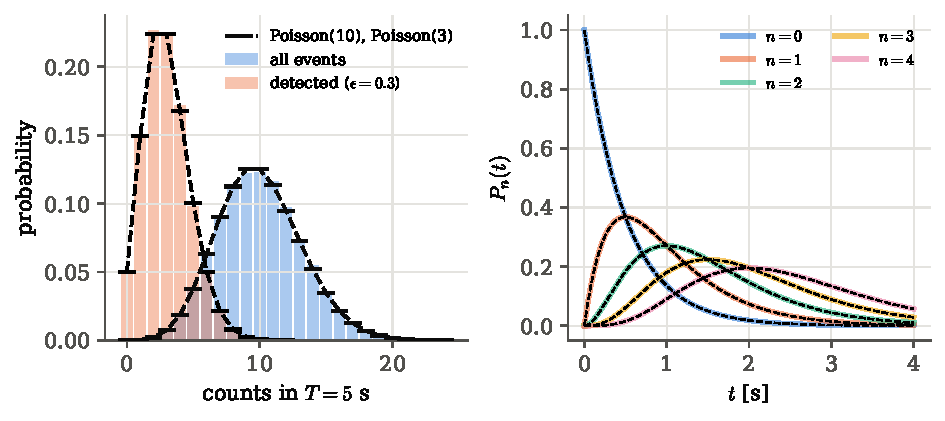
\includegraphics[width=\linewidth]{figures/ch02/05_poisson_process.pdf}
\caption{Left: counts in $5$~s windows built slice by slice, for all events (blue) and for the $30\%$ that are detected (orange); the black ticks are Poisson(10) and Poisson(3). Right: the ladder probabilities $P_0,\dots,P_4$ from integrating the master equation (thick coloured curves) lie on the analytic Poisson curves (thin dashed). $P_0$ decays from one; each higher rung fills up later and peaks at $t=n/\lambda$.}
\label{2a:fig:pp-sim}
\end{figure}

Over $20\,000$ windows the total count has mean $\twoaPPMean$ and variance $\twoaPPVar$ (theory $10$ and $10$), the thinned count $\twoaPPDetMean$ and $\twoaPPDetVar$ (theory $3$ and $3$), and the sum of the two sources $\twoaPPSumMean$ and $\twoaPPSumVar$ (theory $15$ and $15$). Empty windows are rare: with $e^{-10}=\twoaPPZeroTh$ we expect $20\,000\,e^{-10}\approx\twoaPPZeroExpect$ of them, and this run has $\twoaPPZeroCount$. The Euler solution of the master equation differs from $e^{-\lambda t}(\lambda t)^n/n!$ by at most $\twoaPPMaxErr$ over $0\le t\le4$~s (\cref{2a:fig:pp-sim}), an error that shrinks in proportion to the step size.

\begin{inpractice}[verification versus research]
Everything above is \emph{verification}: the simulation checks an analytic result we already had. The same slice-by-slice machinery becomes a research instrument as soon as the inputs (P1)--(P3) are only approximately true and no formula exists: a rate that depends on the recent history (afterpulsing in a PMT, pile-up in a calorimeter), events that trigger other events (cosmic-ray air showers, aftershocks), or a detector whose efficiency depends on the previous hit (\cref{2a:sec:failures}). Then we simulate the process and histogram the counts, and that histogram \emph{is} the sampling distribution $P(S\given\theta)$ fed into the likelihood.
\end{inpractice}

\section{Waiting times: the exponential and gamma distributions}\label{2a:sec:waiting}

The same Geiger counter can be read in two ways. We can count the clicks in fixed windows (\cref{2a:sec:poisson-process}), or we can record the \emph{time} of each click and look at the gaps between them. A timing detector with a photomultiplier does the second: it waits for the first photon, or for the tenth, and its time resolution is set by how much that waiting time fluctuates. A muon stopped in a scintillator waits a random time before it decays. For a Poisson process these waiting times have simple laws. The time to the first event is exponential. The time to the $n$-th event is gamma (also called Erlang). And the ``no memory'' input becomes the statement that a waiting time never ``ages''.

\paragraph{Physical picture: the survival law of an unstable particle.}
An unstable nucleus has no clock inside it. If it has survived a thousand years, its chance of decaying in the next second is the same as on the day it was made. This is why the survival fraction is $e^{-t/\tau}$, and why we can speak of \emph{the} lifetime $\tau$ of a species without saying how old the sample is. The time between Poisson events is the same law: the process never ``remembers'' when the last event happened.

\paragraph{The question, step by step.}
\begin{enumerate}[leftmargin=1.6em,itemsep=1pt]
  \item The first event comes after time $t$ exactly when the window $[0,t]$ is empty. We already know the probability of that.
  \item The $n$-th event comes before time $w$ exactly when the window $[0,w]$ holds at least $n$ events. We know that too.
  \item Differentiate these probabilities to get densities. Compute means and variances.
  \item Check the ``no memory'' property directly, and simulate a stream from its gaps.
\end{enumerate}

\begin{figure}[htbp]
\centering
\begin{tikzpicture}[x=1.05cm]
  \draw[->,thick] (0,0) -- (11,0);
  \node[lbl,anchor=north] at (11,-0.05) {$t$};
  \def\ta{1.4}\def\tb{2.3}\def\tc{4.6}\def\td{5.1}\def\te{8.2}
  \foreach \x in {0,\ta,\tb,\tc,\td,\te}{\draw[thick] (\x,-0.12) -- (\x,0.12);}
  \foreach \x in {\ta,\tb,\tc,\td,\te}{\fill[bdryred] (\x,0) circle (2.2pt);}
  \draw[decorate,decoration={brace,amplitude=4pt},tangentgreen,thick] (0,0.25) -- (\ta,0.25);
  \node[font=\scriptsize,tangentgreen,anchor=south] at ({\ta/2},0.42) {$S_0$};
  \draw[decorate,decoration={brace,amplitude=4pt},tangentgreen,thick] (\ta,0.25) -- (\tb,0.25);
  \node[font=\scriptsize,tangentgreen,anchor=south] at ({(\ta+\tb)/2},0.42) {$S_1$};
  \draw[decorate,decoration={brace,amplitude=4pt},tangentgreen,thick] (\tb,0.25) -- (\tc,0.25);
  \node[font=\scriptsize,tangentgreen,anchor=south] at ({(\tb+\tc)/2},0.42) {$S_2$};
  \draw[decorate,decoration={brace,amplitude=4pt},tangentgreen,thick] (\tc,0.25) -- (\td,0.25);
  \node[font=\scriptsize,tangentgreen,anchor=south] at ({(\tc+\td)/2},0.42) {$S_3$};
  \draw[decorate,decoration={brace,amplitude=4pt},tangentgreen,thick] (\td,0.25) -- (\te,0.25);
  \node[font=\scriptsize,tangentgreen,anchor=south] at ({(\td+\te)/2},0.42) {$S_4$};
  \foreach \x/\n in {\ta/1,\tb/2,\tc/3,\td/4,\te/5}{\node[font=\scriptsize,anchor=north] at (\x,-0.15) {$W_{\n}$};}
  \node[font=\scriptsize,anchor=north] at (0,-0.15) {$0$};
  \draw[decorate,decoration={brace,amplitude=5pt,mirror},formblue,thick] (0,-0.65) -- (\tc,-0.65);
  \node[font=\scriptsize,formblue,anchor=north] at ({\tc/2},-0.85) {$W_3=S_0+S_1+S_2$};
  \draw[fibreorange,thick,dashed] (6.5,-0.45) -- (6.5,0.2);
  \node[font=\scriptsize,fibreorange,anchor=west] at (6.55,-0.75) {at $t=6.5$: $N(t)=4$};
\end{tikzpicture}
\caption{One stretch of a Poisson stream. The green braces are the gaps (sojourn times) $S_0,S_1,\dots$ between successive events; the arrival times $W_n$ are their running sums. At the dashed line four events have happened, so $W_4\le t<W_5$: counts and waiting times are two descriptions of the same stream.}
\label{2a:fig:gaps}
\end{figure}

\subsection{The first event: exponential}

Let $T=W_1$ be the time of the first event, and recall that $N(t)$ is the number of events in $[0,t]$. \Cref{2a:fig:gaps} shows the link between the two descriptions: the first event comes after $t$ if and only if there is no event in $[0,t]$, that is, $T>t$ exactly when $N(t)=0$. This duality between waiting times and counts turns a question about times into one about counts, which we have already answered. So
\begin{align}
  \Prob(T>t) \eqby{1} \Prob(N(t)=0) \eqby{2} e^{-\lambda t},\qquad
  F(t)=\Prob(T\le t)=1-e^{-\lambda t},\qquad
  f(t) \eqby{3} \frac{\dd F}{\dd t}=\lambda e^{-\lambda t}. \label{2a:eq:expo}
\end{align}
\begin{explain}
  \item The duality between waiting times and counts.
  \item The empty-window probability $P_0(t)$ from \cref{2a:sec:poisson-process}.
  \item A density is the derivative of the CDF (\cref{ch:01}).
\end{explain}

\begin{workdef}[exponential distribution]
$T\sim\mathrm{Exp}(\lambda)$ in the \emph{rate} parameterisation if $f(t)=\lambda e^{-\lambda t}$ for $t\ge0$ \unpack{$\lambda$ is events per unit time}; equivalently, in the \emph{scale} parameterisation used by AoS, $f(t)=\frac1\beta e^{-t/\beta}$ with $\beta=1/\lambda$ \unpack{$\beta$ is a time, the mean wait}. For a decaying particle $\beta=\tau$, the mean lifetime.
\emph{Recognise it by:} the waiting time until something that happens at a constant rate and does not age.
\end{workdef}

The moments of the exponential, and those of the gamma distribution below, need one special function. The \newterm{gamma function} is, for $\alpha>0$, $\Gamma(\alpha)=\int_0^\infty y^{\alpha-1}e^{-y}\,\dd y$ \unpack{a continuous extension of the factorial, with $\Gamma(n)=(n-1)!$}.
Its three essential properties:
\begin{align*}
  \Gamma(1) &= \int_0^\infty e^{-y}\dd y = 1,\\
  \Gamma(\alpha+1) &\eqby{1} \Bigl[-y^\alpha e^{-y}\Bigr]_0^\infty+\alpha\int_0^\infty y^{\alpha-1}e^{-y}\dd y \eqby{2} \alpha\,\Gamma(\alpha),\\
  \Gamma(\tfrac12) &\eqby{3} \int_0^\infty y^{-1/2}e^{-y}\dd y \eqby{4} 2\int_0^\infty e^{-x^2}\dd x = \sqrt\pi .
\end{align*}
\begin{explain}
  \item Integration by parts, with $u=y^\alpha$ and $\dd v=e^{-y}\dd y$.
  \item The boundary term vanishes at both ends for $\alpha>0$.
  \item Definition with $\alpha=\tfrac12$.
  \item Substitute $y=x^2$, $\dd y=2x\,\dd x$, and use the Gaussian integral $\int_{-\infty}^\infty e^{-x^2}\dd x=\sqrt\pi$.
\end{explain}
From the first two, $\Gamma(n)=(n-1)(n-2)\cdots1\cdot\Gamma(1)=(n-1)!$ for integer $n$ \srcref{CasellaBerger}{(3.3.2)--(3.3.4), p.~81}.

Now the moments of the exponential, substituting $y=\lambda t$:
\begin{align*}
  \E T^r \eqby{1} \int_0^\infty t^r\lambda e^{-\lambda t}\dd t \eqby{2} \frac1{\lambda^r}\int_0^\infty y^re^{-y}\dd y \eqby{3} \frac{\Gamma(r+1)}{\lambda^r}=\frac{r!}{\lambda^r}.
\end{align*}
\begin{explain}
  \item Definition of the $r$-th moment.
  \item $t=y/\lambda$, $\dd t=\dd y/\lambda$.
  \item Definition of $\Gamma(r+1)$.
\end{explain}
So $\E T=1/\lambda$, $\E T^2=2/\lambda^2$ and $\Var T=2/\lambda^2-1/\lambda^2=1/\lambda^2$. The mean waiting time is the inverse rate, and the standard deviation equals the mean: an exponential wait is as uncertain as it is long.

\subsection{No memory}

\begin{keyidea}[the exponential is memoryless]
For all $t,s\ge0$, $\Prob(T>t+s\given T>t)=\Prob(T>s)$.
\end{keyidea}
\begin{align*}
  \Prob(T>t+s\given T>t) \eqby{1} \frac{\Prob(T>t+s\text{ and }T>t)}{\Prob(T>t)} \eqby{2} \frac{\Prob(T>t+s)}{\Prob(T>t)} \eqby{3} \frac{e^{-\lambda(t+s)}}{e^{-\lambda t}} = e^{-\lambda s} = \Prob(T>s).
\end{align*}
\begin{explain}
  \item Definition of conditional probability (\cref{ch:01}).
  \item $T>t+s$ already implies $T>t$.
  \item Survival function \eqref{2a:eq:expo}.
\end{explain}
In words: having waited a time $t$ without an event, the remaining wait has the same distribution as a fresh one (\cref{2a:fig:memoryless}). The converse is also true: the exponential is the \emph{only} continuous distribution with this property. To see why, write $G(t)=\Prob(T>t)$ for the survival function. Memorylessness says $G(t+s)/G(t)=G(s)$, that is, $G(t+s)=G(t)G(s)$. Taking logarithms, $\ln G(t+s)=\ln G(t)+\ln G(s)$: the function $\ln G$ is additive. The only continuous additive functions are linear, so $\ln G(t)=-\lambda t$ for some constant $\lambda>0$. So memorylessness \emph{forces} $G(t)=e^{-\lambda t}$ \srcref{CasellaBerger}{(3.3.11), p.~83}.

\begin{figure}[htbp]
\centering
\begin{tikzpicture}
\begin{axis}[width=10cm,height=5cm,xmin=0,xmax=3,ymin=0,ymax=1.08,
  xlabel={$t$ [s]},ylabel={$\Prob(T>t)=e^{-2t}$},axis lines=left,
  tick label style={font=\scriptsize},label style={font=\small},
  xtick={0,0.5,1,1.5,2,2.5,3},ytick={0,0.135,0.368,0.5,1},
  yticklabels={$0$,$0.135$,$0.368$,$0.5$,$1$}]
  \addplot[thick,formblue,domain=0:3,samples=120] {exp(-2*x)};
  \addplot[thick,tangentgreen] coordinates {(0.5,0) (0.5,0.3679)};
  \addplot[only marks,mark=*,mark size=1.6pt,tangentgreen] coordinates {(0.5,0.3679)};
  \addplot[thick,bdryred] coordinates {(1,0) (1,0.1353)};
  \addplot[thick,bdryred,dashed] coordinates {(1.5,0) (1.5,0.0498)};
  \addplot[only marks,mark=*,mark size=1.6pt,bdryred] coordinates {(1,0.1353) (1.5,0.0498)};
  \addplot[faint,dashed] coordinates {(0,0.3679) (0.5,0.3679)};
  \addplot[faint,dashed] coordinates {(0,0.1353) (1,0.1353)};
  \node[font=\scriptsize,tangentgreen,anchor=west] at (axis cs:0.55,0.45) {$\Prob(T>0.5)=0.368$};
  \node[font=\scriptsize,bdryred,anchor=west] at (axis cs:1.55,0.2) {$\dfrac{\Prob(T>1.5)}{\Prob(T>1)}=\dfrac{0.0498}{0.1353}=0.368$};
\end{axis}
\end{tikzpicture}
\caption{The survival curve of an exponential wait with $\lambda=2$~s$^{-1}$. The chance of waiting a further half second is the same whether we start the clock at zero (green: height at $0.5$) or after an empty first second (red: ratio of the heights at $1.5$ and $1$). Every stretch of the curve is a scaled copy of the whole.}
\label{2a:fig:memoryless}
\end{figure}

\paragraph{The gaps are independent exponentials.} Recall from \cref{2a:fig:gaps} that $S_0,S_1,\dots$ are the gaps between successive events and $W_n$ is the time of the $n$-th event. The argument for the first wait restarts at every event. Given that the first event is at $W_1=s$, the second gap $S_1$ exceeds $t$ exactly when $(s,s+t]$ is empty:
\begin{align*}
  \Prob(S_1>t\given W_1=s) \eqby{1} \Prob(\text{no events in }(s,s+t]\given W_1=s) \eqby{2} \Prob(\text{no events in }(s,s+t]) \eqby{3} e^{-\lambda t}.
\end{align*}
\begin{explain}
  \item Duality between the gap and an empty interval.
  \item Independent increments: what happens in $(s,s+t]$ does not care about $[0,s]$.
  \item Stationarity: an interval of length $t$ is empty with probability $e^{-\lambda t}$ wherever it sits.
\end{explain}
The answer does not depend on $s$, so $S_1$ is independent of $W_1=S_0$ and is again Exp$(\lambda)$. Repeating the argument, the gaps $S_0,S_1,S_2,\dots$ are independent and identically distributed (iid) Exp$(\lambda)$ \mainref{Thm.~23.35, p.~396}. This gives a second, equivalent definition of the Poisson process: \emph{a stream of events whose gaps are iid exponential}. It is the one we use to simulate.

\subsection{The $n$-th event: gamma (Erlang)}

The time of the $n$-th event is $W_n=S_0+S_1+\dots+S_{n-1}$, a sum of $n$ independent exponentials. Use the duality again: $W_n\le w$ exactly when at least $n$ events happened by $w$.
\begin{align}
  \Prob(W_n\le w) &\eqby{1} \Prob(N(w)\ge n) \eqby{2} 1-\sum_{k=0}^{n-1}e^{-\lambda w}\frac{(\lambda w)^k}{k!}, \nonumber\\
  f_{W_n}(w) &\eqby{3} \lambda e^{-\lambda w}\sum_{k=0}^{n-1}\frac{(\lambda w)^k}{k!}-e^{-\lambda w}\sum_{k=1}^{n-1}\frac{\lambda^kw^{k-1}}{(k-1)!} \nonumber\\
  &\eqby{4} \lambda e^{-\lambda w}\Bigl[\sum_{k=0}^{n-1}\frac{(\lambda w)^k}{k!}-\sum_{j=0}^{n-2}\frac{(\lambda w)^j}{j!}\Bigr]
   \eqby{5} \frac{\lambda^n w^{n-1}}{(n-1)!}\,e^{-\lambda w}. \label{2a:eq:erlang}
\end{align}
\begin{explain}
  \item The $n$-th arrival is before $w$ if and only if the count at $w$ is at least $n$.
  \item $N(w)\sim\mathrm{Poisson}(\lambda w)$; complement of $k\le n-1$.
  \item Differentiate with the product rule: the derivative of $e^{-\lambda w}$ gives the first sum (with the sign flipped by the leading minus), the derivative of $(\lambda w)^k/k!$ is $\lambda^kw^{k-1}/(k-1)!$ (zero for $k=0$).
  \item In the second sum take out $\lambda$ and rename $j=k-1$.
  \item The two sums \emph{telescope}: every term cancels except $k=n-1$ in the first.
\end{explain}
This is the \newterm{Erlang} density.\footnote{The density printed in \mainref{Thm.~23.35, p.~396} has $e^{-\lambda t}$ where $e^{-\lambda w}$ is meant. The proof there also writes $S_1$ for the first gap after defining the gaps from $S_0$.} With $\Gamma(n)=(n-1)!$ and the scale $\beta=1/\lambda$ it is a special case of the general gamma family.

\begin{workdef}[gamma distribution]
$X\sim\mathrm{Gamma}(\alpha,\beta)$ (shape $\alpha>0$, scale $\beta>0$) if
\begin{equation}
  f(x\given\alpha,\beta)=\frac{1}{\Gamma(\alpha)\,\beta^\alpha}\,x^{\alpha-1}e^{-x/\beta},\qquad x>0. \label{2a:eq:gamma}
\end{equation}
\unpack{for integer $\alpha=n$ and $\beta=1/\lambda$, the waiting time for the $n$-th event of a rate-$\lambda$ Poisson process}. $\mathrm{Exp}$ is $\mathrm{Gamma}(1,\beta)$.
\emph{Recognise it by:} a sum of independent exponential waits, or more generally a positive quantity whose density rises like a power and falls like an exponential.
\end{workdef}

It is normalised because substituting $y=x/\beta$ turns $\int_0^\infty x^{\alpha-1}e^{-x/\beta}\dd x$ into $\beta^\alpha\Gamma(\alpha)$. Its moments follow from the \emph{kernel trick}: recognise the integrand as another gamma density, up to its constant.
\begin{align*}
  \E X \eqby{1} \int_0^\infty\frac{x^{\alpha}e^{-x/\beta}}{\Gamma(\alpha)\beta^\alpha}\dd x
  \eqby{2} \frac{\Gamma(\alpha+1)\beta^{\alpha+1}}{\Gamma(\alpha)\beta^\alpha}
  \eqby{3} \alpha\beta,\qquad
  \E X^2 \eqby{2} \frac{\Gamma(\alpha+2)\beta^{\alpha+2}}{\Gamma(\alpha)\beta^\alpha}=\alpha(\alpha+1)\beta^2 .
\end{align*}
\begin{explain}
  \item One extra factor of $x$ raises the power to $x^\alpha$.
  \item $\int_0^\infty x^{(\alpha+1)-1}e^{-x/\beta}\dd x=\Gamma(\alpha+1)\beta^{\alpha+1}$, the normalisation of Gamma$(\alpha+1,\beta)$; likewise with $\alpha+2$.
  \item $\Gamma(\alpha+1)=\alpha\Gamma(\alpha)$.
\end{explain}
So $\Var X=\alpha(\alpha+1)\beta^2-\alpha^2\beta^2=\alpha\beta^2$ \srcref{CasellaBerger}{(3.3.7)--(3.3.8), p.~82}. For the Erlang wait, $\E W_n=n/\lambda$ and $\Var W_n=n/\lambda^2$, exactly $n$ times the exponential values, as a sum of $n$ independent gaps must give.

The mgf, by the same substitution, is $M_X(t)=(1-\beta t)^{-\alpha}$ for $t<1/\beta$. Multiplying mgfs shows that independent $\mathrm{Gamma}(\alpha_i,\beta)$ variables with a \emph{common scale} add to $\mathrm{Gamma}(\sum\alpha_i,\beta)$: $n$ gaps of $\mathrm{Gamma}(1,1/\lambda)$ make $\mathrm{Gamma}(n,1/\lambda)$, and the first $n$ gaps followed by the next $m$ make $W_{n+m}$.

\paragraph{The gamma--Poisson identity.} The first line of \eqref{2a:eq:erlang} is a useful identity in its own right. For integer $\alpha$ and $X\sim\mathrm{Gamma}(\alpha,\beta)$,
\[
  \Prob(X\le x)=\Prob(Y\ge\alpha),\qquad Y\sim\mathrm{Poisson}(x/\beta).
\]
A tail probability of a continuous waiting time equals a tail probability of a discrete count \srcref{CasellaBerger}{(3.3.9), p.~82}. Casella and Berger prove it by repeated integration by parts; the duality ``$n$-th event before $x$ $\Leftrightarrow$ at least $n$ events by $x$'' makes it obvious.

\subsection{Worked examples}

\paragraph{Example: muon survival.}
Stopped muons decay with mean lifetime $\tau=2.197~\mu$s. What fraction survives $5~\mu$s? By \eqref{2a:eq:expo} with $\lambda=1/\tau$, $\Prob(T>5~\mu\text{s})=e^{-5/2.197}=\twoaMuonSurv$. By memorylessness, a muon that has already survived $5~\mu$s again has about a $10\%$ chance to survive the next $5~\mu$s. So measuring $\tau$ does not require knowing when each muon was produced. Any start time after the muon stops gives the same exponential shape with the same $\tau$. This is why a muon-lifetime experiment can start its clock at the stop signal and ignore everything earlier.

\paragraph{Example: waiting for the third photon.}
Photons reach a photocathode at $\lambda=2$ per ns (after thinning by the quantum efficiency). The discriminator fires on the third photoelectron. What is the probability that it has fired within $1$~ns? By the gamma--Poisson identity,
\begin{align*}
  \Prob(W_3\le1) \eqby{1} \Prob(N(1)\ge3) \eqby{2} 1-e^{-2}\Bigl(1+2+\frac{2^2}{2}\Bigr) = 1-5e^{-2} = 1-0.677 = 0.323 .
\end{align*}
\begin{explain}
  \item Duality; $N(1)\sim\mathrm{Poisson}(2)$.
  \item Complement of $k=0,1,2$.
\end{explain}
The timing jitter of this trigger is the spread of $W_3$. With $\beta=1/\lambda=0.5$~ns, $W_3\sim\mathrm{Gamma}(3,0.5\text{ ns})$ has mean $\alpha\beta=1.5$~ns and standard deviation $\sqrt{\alpha}\,\beta=\sqrt3\times0.5=0.87$~ns. In general, firing on the $n$-th photon gives mean $n/\lambda$ and standard deviation $\sqrt n/\lambda$, so the relative jitter is $1/\sqrt n$. The more photons we wait for, the later the trigger, but the more \emph{predictable}.

\paragraph{Example: counts or gaps: the same information about $\lambda$.}
We watch a Poisson stream for a time $T$ and see $N$ events at times $w_1<\dots<w_N$. From the counts alone, the probability of the data is $e^{-\lambda T}(\lambda T)^N/N!$. From the gaps: $N$ gaps of the observed lengths (density $\lambda e^{-\lambda s_i}$ each) and then no event in the last stretch $T-w_N$ (probability $e^{-\lambda(T-w_N)}$). The product is
\begin{align*}
  \prod_{i=1}^N\lambda e^{-\lambda s_i}\times e^{-\lambda(T-w_N)} \eqby{1} \lambda^Ne^{-\lambda w_N}e^{-\lambda(T-w_N)} = \lambda^Ne^{-\lambda T}.
\end{align*}
\begin{explain}
  \item The gaps add up to the time of the last event, $\sum_is_i=w_N$.
\end{explain}
As functions of $\lambda$, the count probability and the gap product are both proportional to $\lambda^Ne^{-\lambda T}$ \mainref{Ex.~23.36, p.~396}. So the detailed arrival times carry no information about a constant rate beyond $N$ and $T$. Both likelihoods peak at the same estimate, $\hat\lambda=N/T$ (\cref{ch:03}). The exact times \emph{do} matter as soon as we want to test whether the rate is constant.

\subsection{Python: a stream built from its gaps}

To simulate the gaps we need exponential numbers, made from uniform ones. One fact does it \srcref{Cowan}{(2.16)--(2.18), p.~30}: if $X$ has a continuous CDF $F$, then $U=F(X)$ is uniform on $[0,1]$. Reading it backwards, $X=F^{-1}(U)$ has CDF $F$. For the exponential, $U=1-e^{-\lambda T}$ gives $T=-\ln(1-U)/\lambda$. Since $1-U$ is also uniform, $T=-\ln U/\lambda$ does the same job. This is \emph{inverse-transform sampling}, developed in general in \cref{ch:06}.

\pyfile[firstline=23,lastline=31,firstnumber=23]{code/ch02/06_waiting_times.py}{Exponential gaps, arrival times, counts per window}

Line 24 draws $200\,000$ exponential gaps with $\lambda=2$~s$^{-1}$; line 25 turns them into arrival times by a running sum, exactly as in \cref{2a:fig:gaps}. Line 27 counts the arrivals in each $1$~s window: \pyname{np.floor(times)} is the window index of each event and \pyname{np.bincount} counts events per index. The function \pyname{erlang_pdf} is \eqref{2a:eq:erlang}. Further down, the gaps are grouped in blocks of $n$ and summed to give samples of $W_n$.

\begin{figure}[htbp]
\centering
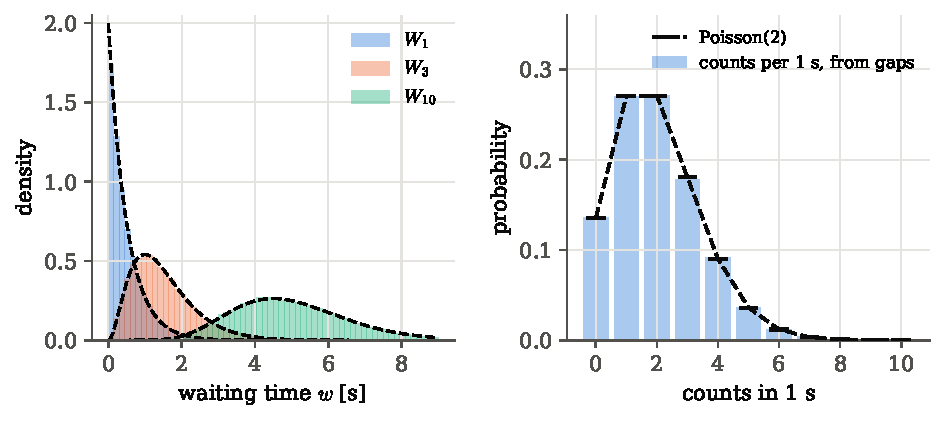
\includegraphics[width=\linewidth]{figures/ch02/06_waiting_times.pdf}
\caption{Left: histograms of the arrival time of the first, third and tenth event, built by summing $1$, $3$ or $10$ simulated gaps, with the Erlang densities as dashed curves. The first arrival is most likely immediately; later arrivals have a peak that moves right and a width that grows only like $\sqrt n$. Right: counting the same stream in $1$~s windows gives the Poisson(2) distribution, closing the loop from gaps back to counts.}
\label{2a:fig:wait-sim}
\end{figure}

The gaps have sample mean $\twoaWTGapMean$~s and variance $\twoaWTGapVar$~s$^2$ (theory $1/\lambda=0.5$ and $1/\lambda^2=0.25$). The counts per second have mean $\twoaWTCountMean$ and variance $\twoaWTCountVar$ (theory $2$ and $2$). The tenth arrival has mean $\twoaWTWtenMean$~s and variance $\twoaWTWtenVar$~s$^2$ (theory $5$ and $2.5$). For memorylessness, among the gaps that exceeded $1$~s the fraction that exceeded $1.5$~s is $\twoaWTCond$, against $\twoaWTUncond$ for all gaps exceeding $0.5$~s and the theoretical $e^{-1}=\twoaWTMemTh$ (\cref{2a:fig:wait-sim}).

\begin{pitfall}[rate or scale? three conventions for one distribution]
The same gamma distribution is written with a \emph{scale} $\beta$ (AoS, Casella--Berger, \pyname{scipy.stats.gamma(a, scale=beta)}, \pyname{numpy}'s \pyname{rng.gamma(shape, scale)}), or with a \emph{rate} $1/\beta$ (Lambert, most Bayesian texts and Stan). ``Exp(2)'' means mean $2$ in one book and mean $1/2$ in another. Always check by computing the mean. Lambert's lottery example is a warning: three prize-claiming times, each exponential with rate $1$ per day, sum to a gamma with \emph{shape} $3$ and rate $1$, which the text describes with the words ``scale'' and ``shape'' swapped \srcref{Lambert}{\S8.4.9}.
\end{pitfall}

\paragraph{Not every lifetime is exponential.} Memorylessness means a constant \emph{hazard} $h(t)=f(t)/\Prob(T>t)$ \unpack{the probability per unit time of failing now, given survival so far}. For the exponential $h(t)=\lambda$. Components that wear out have a rising hazard and are better described by the Weibull distribution, $\Prob(T>t)=e^{-(t/\beta)^\gamma}$ with $\gamma>1$ \srcref{CasellaBerger}{(3.3.12), p.~83}. Particles and nuclei have no wear, which is why the exponential law of decay is exact (to the extent quantum mechanics allows).

\section{Discrete waiting times and extra spread: geometric and negative binomial}\label{2a:sec:negbin}

At a collider, bunches cross every $25$~ns and each crossing fires a rare trigger with probability $p$. How many crossings do we wait until the first trigger? Until the third? This is the waiting-time question of \cref{2a:sec:waiting}, but with time coming in discrete ticks. A second puzzle has the same answer. A galaxy survey counts galaxies in cells of equal volume. The mean is $10$ per cell, but the variance is $30$, not the $10$ a Poisson count would have. The counts are \emph{overdispersed}: they scatter more than Poisson, because galaxies cluster and the underlying density varies from cell to cell. Two distributions answer both questions. The geometric and negative binomial distributions count trials until a given number of successes. The negative binomial then reappears as a Poisson count whose mean itself fluctuates, and in that role it is the standard model for counts that scatter more than Poisson.

\paragraph{Physical picture: ticks of a clock, and a Poisson with a wobbling rate.}
The geometric wait is the exponential wait with time chopped into ticks; shrink the ticks and it becomes the exponential. The overdispersed count is a Poisson count seen through a fluctuating medium, in two stages. First nature picks the local rate. Then a Poisson count is drawn with that rate. The total scatter is the sum of the scatter from the two stages: the Poisson ``shot noise'' plus the variance of the rate. Photon counts from a twinkling star behave this way.

\paragraph{The question, step by step.}
\begin{enumerate}[leftmargin=1.6em,itemsep=1pt]
  \item The first success is on trial $k$ exactly when trials $1,\dots,k-1$ fail and trial $k$ succeeds. Multiply.
  \item The $r$-th success is on trial $x$ exactly when trial $x$ succeeds and the first $x-1$ trials contain $r-1$ successes. That is a binomial count times one more trial.
  \item If a Poisson mean is itself random, average the Poisson pmf over its distribution (marginalise).
\end{enumerate}

\begin{figure}[htbp]
\centering
\begin{tikzpicture}[sq/.style={draw,minimum size=5.5mm,inner sep=0pt,font=\scriptsize}]
  \node[font=\small,anchor=east] at (-0.3,0) {geometric};
  \foreach \i in {1,...,6}{\node[sq,fill=softgray!20] at ({(\i-1)*0.62},0) {F};}
  \node[sq,fill=formblue!40] at (3.72,0) {S};
  \node[font=\scriptsize,anchor=west] at (4.2,0) {first success on trial $k=7$};
  \node[font=\small,anchor=east] at (-0.3,-1.1) {neg.\ binomial};
  \foreach \i/\c in {1/F,2/S,3/F,4/F,5/F,6/S,7/F,8/F,9/F,10/F}{
    \if S\c
      \node[sq,fill=formblue!40] at ({(\i-1)*0.62},-1.1) {S};
    \else
      \node[sq,fill=softgray!20] at ({(\i-1)*0.62},-1.1) {F};
    \fi}
  \node[sq,fill=formblue!40,draw=bdryred,thick] at (6.2,-1.1) {S};
  \node[font=\scriptsize,anchor=west] at (6.7,-1.1) {third success on trial $x=11$};
  \draw[decorate,decoration={brace,amplitude=4pt,mirror},thick,accent] (-0.28,-1.5) -- (5.86,-1.5);
  \node[font=\scriptsize,accent,anchor=north] at (2.8,-1.7) {first $x-1=10$ trials: any arrangement of $r-1=2$ successes, $\binom{10}{2}$ ways};
\end{tikzpicture}
\caption{Two waits in a sequence of Bernoulli trials. Top: the first success after six failures. Bottom: the third success (outlined in red) is the last trial; before it, the two earlier successes can sit in any of $\binom{10}2=45$ arrangements among the first ten trials, each equally probable.}
\label{2a:fig:trials-wait}
\end{figure}

\subsection{The geometric distribution}

\begin{workdef}[geometric distribution]
$X\sim\mathrm{Geom}(p)$ if $X$ is the number of the trial on which the first success occurs, in a sequence of independent Bernoulli$(p)$ trials \unpack{$X$ counts the successful trial too, so $X\ge1$}:
\begin{equation}
  \Prob(X=k)=(1-p)^{k-1}p,\qquad k=1,2,3,\dots \label{2a:eq:geom}
\end{equation}
\emph{Recognise it by:} the number of tries until the first success, with a constant chance per try.
\end{workdef}

The formula follows from the first step listed above. The first success is on trial $k$ when $k-1$ failures, each with probability $1-p$, are followed by a success, all independent; multiplying gives $(1-p)^{k-1}p$. Some books (and \pyname{scipy.stats.nbinom}) count instead the number of \emph{failures} before the first success, $Y=X-1\in\{0,1,\dots\}$, with $\Prob(Y=y)=(1-p)^yp$.\footnote{The normalisation check for the geometric distribution in \mainref{pp.~26--27} has a misprint in its middle sum, which is printed as $p\sum_{k\ge1}(1-p)^k$. That sum equals $1-p$, not $1$. The exponent must be $k-1$, as below.}

\paragraph{Geometric series.} Everything follows from $\sum_{j=0}^\infty r^j=\frac1{1-r}$ for $\abs r<1$. Proof: the partial sum $S_n=1+r+\dots+r^n$ satisfies $S_n-rS_n=1-r^{n+1}$, so $S_n=\frac{1-r^{n+1}}{1-r}\to\frac1{1-r}$. Differentiating term by term (allowed inside the radius of convergence) gives $\sum_{j=1}^\infty jr^{j-1}=\frac1{(1-r)^2}$ and $\sum_{j=2}^\infty j(j-1)r^{j-2}=\frac2{(1-r)^3}$. With $r=1-p$:
\begin{align*}
  \sum_{k=1}^\infty\Prob(X=k) &\eqby{1} p\sum_{k=1}^\infty(1-p)^{k-1} \eqby{2} \frac{p}{1-(1-p)}=1,\\
  \E X &\eqby{3} p\sum_{k=1}^\infty k(1-p)^{k-1} \eqby{4} \frac{p}{p^2}=\frac1p,\\
  \E[X(X-1)] &\eqby{3} p(1-p)\sum_{k=2}^\infty k(k-1)(1-p)^{k-2} \eqby{4} \frac{2p(1-p)}{p^3}=\frac{2(1-p)}{p^2},\\
  \Var X &\eqby{5} \frac{2(1-p)}{p^2}+\frac1p-\frac1{p^2}=\frac{1-p}{p^2}.
\end{align*}
\begin{explain}
  \item Take out $p$.
  \item Geometric series with $j=k-1$ running from $0$.
  \item Definition of the (factorial) moment; for the second line one factor $(1-p)$ is taken out so that the power is $k-2$.
  \item The differentiated series with $1-r=p$.
  \item $\Var X=\E[X(X-1)]+\E X-(\E X)^2$; put over $p^2$: $2-2p+p-1=1-p$.
\end{explain}
A trigger with $p=0.1$ fires on average every $10$ crossings, with a standard deviation $\sqrt{0.9}/0.1=9.5$ crossings: nearly as large as the mean, just like the exponential.

\paragraph{The tail and no memory.} The first success comes after trial $k$ exactly when the first $k$ trials all fail, so $\Prob(X>k)=(1-p)^k$. Then
\begin{align*}
  \Prob(X>s+t\given X>t) \eqby{1} \frac{\Prob(X>s+t)}{\Prob(X>t)} = \frac{(1-p)^{s+t}}{(1-p)^t} = (1-p)^s = \Prob(X>s)
\end{align*}
\begin{explain}
  \item $X>s+t$ implies $X>t$, and the definition of conditional probability.
\end{explain}
for integers $s,t\ge0$. The geometric is memoryless: a trigger that has not fired for $1000$ crossings is not ``due'' \srcref{CasellaBerger}{(3.2.11), p.~80}.

\paragraph{From ticks to continuous time.} Let the trials be ticks of length $h$ with $p=\lambda h$. The waiting time is $T=hX$, and
\[
  \Prob(T>t)=\Prob(X>t/h)=(1-\lambda h)^{t/h}\xrightarrow{\;h\to0\;}e^{-\lambda t},
\]
by the compound-interest limit of \cref{2a:sec:poisson-limit} with $n=t/h$. The geometric becomes the exponential, just as the binomial became the Poisson. The slices of \cref{2a:fig:slices} are exactly these ticks.

\subsection{The negative binomial}

\begin{workdef}[negative binomial distribution]
In a sequence of independent Bernoulli$(p)$ trials, let $X$ be the number of the trial on which the $r$-th success occurs. Then $X\sim\mathrm{NegBin}(r,p)$ with
\begin{equation}
  \Prob(X=x)=\binom{x-1}{r-1}p^r(1-p)^{x-r},\qquad x=r,r+1,\dots \label{2a:eq:nbx}
\end{equation}
Equivalently, the number of failures before the $r$-th success, $Y=X-r$, has
\begin{equation}
  \Prob(Y=y)=\binom{r+y-1}{y}p^r(1-p)^y,\qquad y=0,1,2,\dots \label{2a:eq:nby}
\end{equation}
\unpack{for $r=1$ these are the two forms of the geometric}.
\emph{Recognise it by:} the number of tries until a fixed number $r$ of successes, or (see below) a count that is more spread out than Poisson.
\end{workdef}

\emph{Derivation of \eqref{2a:eq:nbx}.} This is the second step listed above (\cref{2a:fig:trials-wait}). The $r$-th success is on trial $x$ if and only if two things happen. First, the first $x-1$ trials contain exactly $r-1$ successes; this has the binomial probability $\binom{x-1}{r-1}p^{r-1}(1-p)^{x-r}$. Second, trial $x$ succeeds, with probability $p$, independently of the earlier trials. Multiplying the two gives \eqref{2a:eq:nbx}. Replacing $x=y+r$ and using $\binom{n}{k}=\binom{n}{n-k}$ gives \eqref{2a:eq:nby} \srcref{CasellaBerger}{(3.2.9)--(3.2.10), p.~78}.

\paragraph{Mean and variance: a sum of geometric waits.} After each success the process starts afresh, because the trials are independent. So $Y$, the number of failures before the $r$-th success, is the sum of $r$ independent copies of $Y_1=X_1-1$, the number of failures before the first success; here $X_1\sim\mathrm{Geom}(p)$. From the geometric moments, $Y_1$ has $\E Y_1=\frac1p-1=\frac{1-p}p$ and $\Var Y_1=\Var X_1=\frac{1-p}{p^2}$. Hence
\begin{equation}
  \E Y=\frac{r(1-p)}{p},\qquad \Var Y=\frac{r(1-p)}{p^2}=\E Y+\frac{(\E Y)^2}{r}. \label{2a:eq:nbvar}
\end{equation}
The last form follows by writing $\mu=r(1-p)/p$: then $\mu+\mu^2/r=\frac{r(1-p)}p\bigl(1+\frac{1-p}{p}\bigr)=\frac{r(1-p)}{p^2}$. \emph{The variance always exceeds the mean}, by $\mu^2/r$.

\paragraph{Why ``negative'' binomial.} Write out the coefficient with $r+y-1$ over $y$ and pull out a sign from each of the $y$ factors:
\begin{align*}
  \binom{r+y-1}{y} \eqby{1} \frac{(r+y-1)(r+y-2)\cdots r}{y!}
  \eqby{2} (-1)^y\frac{(-r)(-r-1)\cdots(-r-y+1)}{y!}
  \eqby{3} (-1)^y\binom{-r}{y}.
\end{align*}
\begin{explain}
  \item Cancel $(r-1)!$ from $(r+y-1)!/(y!(r-1)!)$, leaving $y$ factors on top.
  \item Each factor $(r+j)=-(-r-j)$, for $j=0,\dots,y-1$, read in reverse order.
  \item The \emph{generalised} binomial coefficient $\binom{a}{y}=a(a-1)\cdots(a-y+1)/y!$ makes sense for any real $a$, including $a=-r$.
\end{explain}
Newton's binomial series $(1+z)^a=\sum_y\binom ay z^y$ for $\abs z<1$ then normalises \eqref{2a:eq:nby}: $\sum_y\binom{-r}{y}(-(1-p))^yp^r=(1-(1-p))^{-r}p^r=1$. The pmf is a term of a binomial expansion with a negative exponent.

\paragraph{Its mgf and the Poisson limit.} For one geometric failure count, $\E e^{tY_1}=\sum_yp(1-p)^ye^{ty}=p/(1-(1-p)e^t)$ (geometric series, valid for $(1-p)e^t<1$). A sum of $r$ independent copies has the $r$-th power. Now let $r\to\infty$ while holding the mean $r(1-p)/p$ close to a fixed $\lambda$; to leading order $1-p=\lambda/r$:
\begin{align*}
  M_Y(t)=\Bigl(\frac{p}{1-(1-p)e^t}\Bigr)^r
  \eqby{1} \frac{(1-\lambda/r)^r}{(1-\lambda e^t/r)^r}
  \;\xrightarrow{\;r\to\infty\;}\; \frac{e^{-\lambda}}{e^{-\lambda e^t}} = e^{\lambda(e^t-1)} .
\end{align*}
\begin{explain}
  \item Substitute $p=1-\lambda/r$.
\end{explain}
The limit is the Poisson mgf \eqref{2a:eq:poismgf}: with many required successes and rare failures, the failure count becomes Poisson, and the excess variance $\mu^2/r$ disappears \srcref{CasellaBerger}{p.~79}.

\subsection{A Poisson count with a fluctuating mean}

The most important appearance of the negative binomial in physics is not about waiting at all. Suppose the count in a cell is Poisson with mean $\Lambda$, but $\Lambda$ itself varies: from cell to cell (clustering), from run to run (beam intensity) or from pixel to pixel (a twinkling source). Take $\Lambda$ to follow a gamma distribution with shape $\kappa$ and scale $\mu/\kappa$. By the gamma moments of \cref{2a:sec:waiting}, $\E\Lambda=\kappa\cdot\mu/\kappa=\mu$ and $\Var\Lambda=\kappa(\mu/\kappa)^2=\mu^2/\kappa$. The distribution of the count is then the \newterm{mixture}: the marginal over the nuisance variable $\Lambda$. Write $\theta=\mu/\kappa$ for the gamma scale:
\begin{align*}
  \Prob(N=n)
  &\eqby{1} \int_0^\infty e^{-\lambda}\frac{\lambda^n}{n!}\;\frac{\lambda^{\kappa-1}e^{-\lambda/\theta}}{\Gamma(\kappa)\theta^\kappa}\,\dd\lambda
  \eqby{2} \frac{1}{n!\,\Gamma(\kappa)\,\theta^\kappa}\int_0^\infty\lambda^{n+\kappa-1}e^{-\lambda(1+\theta)/\theta}\,\dd\lambda\\
  &\eqby{3} \frac{\Gamma(n+\kappa)}{n!\,\Gamma(\kappa)\,\theta^\kappa}\Bigl(\frac{\theta}{1+\theta}\Bigr)^{n+\kappa}
  \eqby{4} \frac{\Gamma(n+\kappa)}{n!\,\Gamma(\kappa)}\Bigl(\frac{\kappa}{\kappa+\mu}\Bigr)^{\kappa}\Bigl(\frac{\mu}{\kappa+\mu}\Bigr)^{n}.
\end{align*}
\begin{explain}
  \item Law of total probability for a continuous nuisance variable: Poisson pmf given $\Lambda=\lambda$, times the gamma density of $\Lambda$, integrated.
  \item Collect the powers of $\lambda$ and the exponentials: $\lambda+\lambda/\theta=\lambda(1+\theta)/\theta$.
  \item The integral is the gamma normalisation with shape $n+\kappa$ and scale $\theta/(1+\theta)$.
  \item $\theta^{-\kappa}(\theta/(1+\theta))^{\kappa}=(1+\theta)^{-\kappa}$, and $\theta/(1+\theta)=\mu/(\kappa+\mu)$, $1/(1+\theta)=\kappa/(\kappa+\mu)$.
\end{explain}
For integer $\kappa$, $\Gamma(n+\kappa)/(n!\,\Gamma(\kappa))=\binom{\kappa+n-1}{n}$, and this is \eqref{2a:eq:nby} with $r=\kappa$ and $p=\kappa/(\kappa+\mu)$. The formula makes sense for any real $\kappa>0$, and in this role $\kappa$ is called the \newterm{inverse dispersion} \srcref{Lambert}{\S8.4.4}.

The variance is cleanest by the law of total variance (\cref{ch:01}). It splits the scatter into the two stages of the physical picture above: nature picks the rate, then the Poisson count is drawn.
\begin{align}
  \Var N \eqby{1} \E\bigl[\Var(N\given\Lambda)\bigr]+\Var\bigl(\E[N\given\Lambda]\bigr) \eqby{2} \E\Lambda+\Var\Lambda \eqby{3} \mu+\frac{\mu^2}{\kappa}. \label{2a:eq:overdisp}
\end{align}
\begin{explain}
  \item Law of total variance: average of the conditional variance plus variance of the conditional mean.
  \item Given $\Lambda$, $N$ is Poisson, so its conditional mean and variance both equal $\Lambda$.
  \item Gamma moments.
\end{explain}
The variance is the Poisson shot noise $\mu$ plus the variance of the rate, $\mu^2/\kappa$. Nothing in the second step used the gamma form: \emph{any} fluctuating mean gives $\Var N=\mu+\Var\Lambda>\mu$. The gamma only makes the full distribution a closed form.

\subsection{Worked examples}

\paragraph{Example: how long until the trigger fires?}
With $p=0.1$ per crossing, what is the probability of waiting more than $30$ crossings for the first trigger? $\Prob(X>30)=(0.9)^{30}=\twoaGeoTailTh$. And for a light bulb that fails on any given day with probability $0.001$, $\Prob(X>30)=0.999^{30}=0.970$: a $97\%$ chance to last a month \srcref{CasellaBerger}{Ex.~3.2.7, p.~80}. By memorylessness, the same $97\%$ applies to the next month of a bulb that has already lasted a year. Real bulbs age, so the geometric is only a rough model for them; a trigger has no memory, so for it the model is exact.

\paragraph{Example: inverse binomial sampling.}
To measure a rare branching fraction $p$ we can fix the number of trials and count successes (binomial), or keep collecting until we have $r$ successes (negative binomial) \srcref{CasellaBerger}{Ex.~3.2.6, p.~79}. Suppose $p=0.02$ and we stop at $r=100$ signal events. The number of events examined is $X=Y+r$ with
\begin{align*}
  \E X \eqby{1} \frac{r}{p}=5000,\qquad \mathrm{sd}(X) \eqby{2} \frac{\sqrt{r(1-p)}}{p}=\frac{\sqrt{98}}{0.02}=495 .
\end{align*}
\begin{explain}
  \item $\E X=\E Y+r=r(1-p)/p+r=r/p$.
  \item $\Var X=\Var Y=r(1-p)/p^2$ from \eqref{2a:eq:nbvar}.
\end{explain}
The relative uncertainty of the stopping point is $\sqrt{1-p}/\sqrt r\approx10\%$, set by $r$ alone. Stopping rules like this matter for inference: \cref{ch:03} and \cref{ch:05} show that the binomial and negative binomial give proportional likelihoods for $p$, so a Bayesian analysis does not care which rule was used, while a p-value does.

\paragraph{Example: counts in cells of a clustered galaxy field.}
Cells of a survey contain on average $\mu=10$ galaxies. If galaxies were placed independently (a Poisson process in space, \cref{2a:sec:poisson-process}), the variance of the cell counts would be $10$. But galaxies trace a fluctuating matter density. The local mean in a cell is $\Lambda=\mu(1+\delta)$, where $\delta$ is the density contrast smoothed over the cell, with variance $\sigma^2_{\text{cell}}$. So $\Var\Lambda=\mu^2\sigma^2_{\text{cell}}$, and by \eqref{2a:eq:overdisp},
\[
  \Var N=\mu+\mu^2\sigma^2_{\text{cell}} .
\]
If $\sigma^2_{\text{cell}}=0.2$, then $\Var N=10+20=30$, three times the Poisson value. This is the gamma--Poisson model with $1/\kappa=\sigma^2_{\text{cell}}$, that is, $\kappa=5$. Read backwards, the formula is a measurement. The \emph{excess} variance of counts in cells over the Poisson value measures the clustering amplitude $\sigma^2_{\text{cell}}$. That excess is the one-point statistic behind the two-point function of \cref{ch:07}. The Poisson term $\mu$ is the \emph{shot noise} that every galaxy power spectrum must subtract.

\subsection{Python: trials one after another, and a wobbling rate}

\pyfile[firstline=23,lastline=35,firstnumber=23]{code/ch02/07_geometric_negbin.py}{Geometric and negative binomial by running trials; the gamma--Poisson mixture}

For each of $50\,000$ experiments the script runs $400$ Bernoulli$(0.1)$ trials (the chance that fewer than three successes occur in $400$ trials is negligible) and finds the trial numbers of the successes with \pyname{np.flatnonzero}. The first one is the geometric wait; the third one minus $r=3$ is the number of failures before the third success. For the mixture, line 34 draws a rate for each run from a gamma distribution with shape $\kappa=5$ and scale $\mu/\kappa$ (numpy's convention is scale), and line 35 draws one Poisson count with that rate.

\begin{figure}[htbp]
\centering
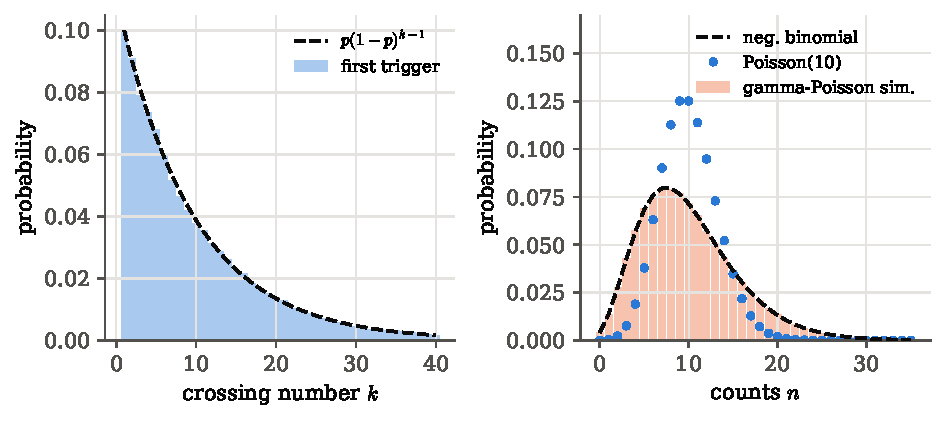
\includegraphics[width=\linewidth]{figures/ch02/07_geometric_negbin.pdf}
\caption{Left: the crossing number of the first trigger (bars) against $p(1-p)^{k-1}$ (dashed): a geometric staircase, highest at $k=1$, falling by a factor $0.9$ per crossing. Right: counts whose Poisson mean wobbles from run to run (bars) follow the negative binomial (dashed), far wider than the Poisson with the same mean $10$ (blue dots).}
\label{2a:fig:nb-sim}
\end{figure}

The geometric wait has sample mean $\twoaGeoMean$ and variance $\twoaGeoVar$ (theory $1/p=10$ and $(1-p)/p^2=90$); $\twoaGeoTail$ of the experiments waited more than $30$ crossings, against $0.9^{30}=\twoaGeoTailTh$. The failures before the third success have mean $\twoaNBMean$ and variance $\twoaNBVar$ (theory $\twoaNBMeanTh$ and $\twoaNBVarTh$). The mixture counts have mean $\twoaMixMean$ and variance $\twoaMixVar$, against $\mu+\mu^2/\kappa=\twoaMixVarTh$ (\cref{2a:fig:nb-sim}).

\paragraph{What this bought us.}
Discrete waits (geometric, negative binomial) are the tick-by-tick versions of the exponential and gamma. The negative binomial also describes a Poisson count with a gamma-distributed mean, with variance $\mu+\mu^2/\kappa$. Whenever counts scatter more than their mean, look for a fluctuating rate.

\section{When the Poisson assumptions fail, and where the Poisson goes for large \texorpdfstring{$\lambda$}{lambda}}\label{2a:sec:failures}

Point a Geiger counter at a radioactive source and move it closer. At first the count rate rises like $1/r^2$, as the solid angle says it should. Closer in, it rises more slowly than $1/r^2$, and with some counters, very close to a strong source, it even \emph{falls}. Now look at the counts in successive short windows at a fixed distance. A second oddity appears: at high rate they scatter \emph{less} than the $\sqrt{\text{mean}}$ that the Poisson distribution promises. A clustered galaxy survey shows the opposite oddity, as we saw in the counts-in-cells example of \cref{2a:sec:negbin}: the counts in cells scatter \emph{more} than Poisson.

Both oddities are the Poisson inputs of \cref{2a:sec:poisson-process} failing, in opposite directions. Each physical effect breaks a particular input (P1)--(P3) of \cref{2a:sec:poisson-inputs}. One number computed from the data detects the failure. And the commonest failure in counting detectors, dead time, can be corrected. A separate question concerns large means: there the Poisson distribution becomes close to a Gaussian, and the replacement is safe in some places and badly wrong in others.

\paragraph{The questions.}
\begin{enumerate}[leftmargin=1.6em,itemsep=1pt]
  \item Which Poisson input does each physical effect break, and does it push the variance of the counts up or down?
  \item Given a set of counts, how do we test whether they are Poisson?
  \item For a counter that is blind for a time $\tau$ after each hit, what is the recorded rate, how do we get the true rate back, and how much do the recorded counts scatter?
  \item For large $\lambda$, how close is Poisson$(\lambda)$ to the Gaussian $\Normal(\lambda,\lambda)$, and where does the approximation fail?
\end{enumerate}

\subsection{Three inputs, two directions of failure}

Recall the three physical inputs from which the Poisson process was derived (\cref{2a:sec:poisson-inputs}):
\begin{enumerate}[leftmargin=2.6em,itemsep=1pt,label=(P\arabic*)]
  \item what happens in one time slice is independent of what happened in all the others \unpack{no memory, no triggering, no suppression};
  \item the rate $\lambda$ is the \emph{same} at all times \unpack{the source does not drift};
  \item events come one at a time \unpack{never two at the same instant}.
\end{enumerate}
From these came the pmf $e^{-\lambda t}(\lambda t)^n/n!$ for the count $N$ in a window of length $t$, and with it the defining fingerprint $\Var N=\E N$. The Poisson is the distribution of ``counts of rare events'' \mainref{p.~27}. Here ``rare'' means precisely that the events do not interact with each other and are not modulated by anything. The same point holds from the user's side \srcref{Lambert}{\S8.4.3}: the mean and the variance are the same parameter, so the Poisson is useful only for data with $\Var N\approx\E N$.

Real effects break the inputs in one of two directions.

\paragraph{More spread than Poisson (overdispersion).} Two kinds of effect make the counts clump.
\begin{itemize}[leftmargin=1.4em,itemsep=1pt]
  \item \emph{The rate itself fluctuates} (input P2 fails). The beam intensity drifts from run to run, the sky background varies across the field, the density of dark matter modulates where galaxies form. In \cref{2a:sec:negbin} we proved that a Poisson count with a random mean $\Lambda$ has $\Var N=\E\Lambda+\Var\Lambda$, eq.~\eqref{2a:eq:overdisp}. The extra term can only add.
  \item \emph{Events trigger further events} (input P1 fails in the positive direction). A photomultiplier pulse is followed by an afterpulse from an ion drifting back to the photocathode. A cosmic-ray primary makes an air shower of secondaries. Events arrive in bunches, and a window either catches a bunch or misses it.
\end{itemize}
The binomial has the same failure mode. When the success probability $p$ varies from group to group, for example between detector modules or between clinical trials, the number of successes is spread wider than $np(1-p)$. Its standard model is the beta-binomial, the binomial analogue of the negative binomial \srcref{Lambert}{\S8.4.5}.

\paragraph{Less spread than Poisson (underdispersion).} Other effects make the events avoid each other, so that the stream becomes more regular than random.
\begin{itemize}[leftmargin=1.4em,itemsep=1pt]
  \item \emph{Events suppress further events} (input P1 fails in the negative direction). After recording a hit the counter is blind for a \newterm{dead time} $\tau$. A neuron cannot fire again during its refractory period. Pile-up rejection throws away events that come too close together.
  \item \emph{The pool of possible events is finite.} With $n$ nuclei and decay probability $p$ per window the count is binomial, with $\Var N=np(1-p)<np=\E N$. This is negligible for a macroscopic source ($n\sim10^{20}$), but not for a handful of trapped ions, or for a short-lived isotope that decays appreciably during the measurement (then input P2 fails as well: the rate falls with time).
\end{itemize}
Input (P3) fails when two events in one slice are recorded as one. This \newterm{pile-up} (two photons in one X-ray CCD pixel within one readout frame, two particles in one calorimeter cell in one bunch crossing) loses events and distorts the recorded energies. As far as the counts are concerned, it acts like a dead time of one frame.

\begin{figure}[htbp]
\centering
\begin{tikzpicture}[x=1.05cm,y=1cm,
  ev/.style={formblue,line width=1.1pt},
  cnt/.style={font=\scriptsize,softgray},
  rowlab/.style={font=\small,anchor=east,align=right}]
  \foreach \xx in {0,2,4,6,8,10} \draw[faint,dashed] (\xx,0.45) -- (\xx,-2.75);
  \node[rowlab] at (-0.2,0) {Poisson\\[-2pt]{\scriptsize independent}};
  \draw[black!40] (0,0) -- (10,0);
  \foreach \t in {0.09,0.48,0.52,1.22,1.23,1.86,2.07,3.30,3.69,3.74,4.32,4.97,6.27,6.33,6.74,6.80,7.85,8.27,8.47,8.53,9.79,9.87}
    \draw[ev] (\t,-0.22) -- (\t,0.22);
  \foreach \xx/\c in {1/6,3/4,5/2,7/5,9/5} \node[cnt] at (\xx,-0.42) {$\c$};
  \node[rowlab] at (-0.2,-1.1) {clustered\\[-2pt]{\scriptsize overdispersed}};
  \draw[black!40] (0,-1.1) -- (10,-1.1);
  \foreach \t in {2.59,2.68,2.91,4.31,4.33,4.34,4.44,4.65,5.19,5.37,8.73,8.77,8.78,8.86,8.93,8.99,9.06,9.08,9.72,9.85}
    \draw[ev,fibreorange] (\t,-1.32) -- (\t,-0.88);
  \foreach \xx/\c in {1/0,3/3,5/7,7/0,9/10} \node[cnt] at (\xx,-1.52) {$\c$};
  \node[rowlab] at (-0.2,-2.2) {regular\\[-2pt]{\scriptsize underdispersed}};
  \draw[black!40] (0,-2.2) -- (10,-2.2);
  \foreach \t in {0.42,0.79,1.13,1.55,1.99,2.60,3.01,3.48,3.98,4.41,4.76,5.26,5.73,6.31,6.90,7.24,7.64,8.07,8.48,8.85,9.47,9.87}
    \draw[ev,tangentgreen] (\t,-2.42) -- (\t,-1.98);
  \foreach \xx/\c in {1/5,3/4,5/4,7/4,9/5} \node[cnt] at (\xx,-2.62) {$\c$};
\end{tikzpicture}
\caption{Three streams of about twenty events, each cut into five equal windows (dashed lines); the small numbers are the counts per window. Top: a Poisson stream, with the irregular gaps and chance near-coincidences of genuine randomness. Middle: the same kind of stream in clumps (a few independent ``parents'', each with a small bunch of offspring): whole windows are empty and others are crowded. Bottom: a dense Poisson stream passed through a counter that is blind for a fixed time after each recorded hit: no two events are close, the gaps are almost equal, and the counts barely change from window to window.}
\label{2a:fig:three-streams}
\end{figure}

\Cref{2a:fig:three-streams} shows the three kinds of stream. The eye reads clumping and regularity immediately. What we need is a number that does the same for a data set of thousands of windows.

\subsection{The Fano factor: a one-number test}

Since a Poisson count has variance equal to its mean, the natural diagnostic is their ratio.

\begin{workdef}[Fano factor (index of dispersion)]
For a count $N$ with mean $\mu>0$, the \newterm{Fano factor} is
\[
  F=\frac{\Var N}{\E N} .
\]
$F=1$ for a Poisson count, $F>1$ is \newterm{overdispersion} \unpack{clumped events or a fluctuating rate}, and $F<1$ is \newterm{underdispersion} \unpack{events that avoid each other, or a finite pool}. From $k$ independent counts $n_1,\dots,n_k$ of the same window we estimate it by
\[
  \hat F=\frac{s^2}{\bar n},\qquad \bar n=\frac1k\sum_{i=1}^kn_i,\quad s^2=\frac1{k-1}\sum_{i=1}^k(n_i-\bar n)^2 .
\]
For Poisson counts with $\bar n\gg1$, $\hat F$ scatters about $1$ with standard deviation $\sqrt{2/(k-1)}$.
\end{workdef}

Values of $F$ we already know: Poisson $F=1$; binomial $F=1-p$; negative binomial $F=1+\mu/\kappa$, from \eqref{2a:eq:overdisp}. The name comes from the physics of ionisation detectors, where U.~Fano showed that the number of electron--ion pairs made by a particle of fixed energy fluctuates less than Poisson (the energy budget is fixed, so the pairs are not independent). The same ratio minus one is Mandel's $Q$ parameter in quantum optics (see the example on sub-Poissonian light below).

\paragraph{How far from $1$ is ``significantly'' far?} A sample Fano factor is itself a random number, so a measured $\hat F=0.97$ need not mean anything. To judge it we need the spread of $\hat F$ when the counts really are Poisson. Two facts give it. The first: for any independent sample of size $k$, the sample variance $s^2$ has
\[
  \Var(s^2)=\frac{2\sigma^4}{k-1}+\frac{\kappa_4}{k},
\]
where $\sigma^2$ is the variance and $\kappa_4$ the fourth \newterm{cumulant} \unpack{the excess of the fourth central moment over its Gaussian value, $\kappa_4=\E(N-\mu)^4-3\sigma^4$} of one count. The first term is the Gaussian result, derived with the $\chi^2$ distribution in the next part. The second is the correction for a non-Gaussian parent. The second fact: for a Poisson count every cumulant equals $\lambda$ (proved in \cref{2a:sec:gauss-preview} below), so $\sigma^2=\kappa_4=\lambda$. The mean $\bar n$ fluctuates by only a relative $1/\sqrt{k\lambda}$, so in the ratio we may treat it as the constant $\lambda$. Then
\begin{align}
  \mathrm{sd}(\hat F)
  &\eqby{1} \frac{\mathrm{sd}(s^2)}{\lambda}
  \eqby{2} \frac1\lambda\sqrt{\frac{2\lambda^2}{k-1}+\frac{\lambda}{k}}
  \eqby{3} \sqrt{\frac{2}{k-1}+\frac{1}{k\lambda}}
  \relby{4}{\approx} \sqrt{\frac{2}{k-1}} . \label{2a:eq:fanosd}
\end{align}
\begin{explain}
  \item $\hat F=s^2/\bar n$ with $\bar n$ replaced by its expected value $\lambda$; its relative fluctuation $1/\sqrt{k\lambda}$ is tiny next to that of $s^2$.
  \item The variance of $s^2$ with $\sigma^2=\kappa_4=\lambda$.
  \item Take $\lambda^2$ out of the square root.
  \item For $\lambda\gg1$ the second term is negligible: $1/(k\lambda)\ll2/(k-1)$.
\end{explain}
The spread depends only on the number of windows $k$, not on the rate. The combination $D=(k-1)\hat F=\sum_i(n_i-\bar n)^2/\bar n$ is the classical \newterm{index-of-dispersion statistic}. For Poisson counts it is close to a $\chi^2$ variable with $k-1$ degrees of freedom, and using it to reject ``the counts are Poisson'' is a hypothesis test in the sense of \cref{ch:04}.

\paragraph{Example: reading a Fano factor.} We record $k=4000$ windows. By \eqref{2a:eq:fanosd}, $\mathrm{sd}(\hat F)=\sqrt{2/3999}=0.0224$.
\begin{itemize}[leftmargin=1.4em,itemsep=1pt]
  \item $\hat F=0.96$ is $(0.96-1)/0.0224=-1.8$ standard deviations from $1$. That happens by chance in about $7\%$ of Poisson data sets (two-sided), so it is no evidence against Poisson.
  \item $\hat F=0.62$ is $-17$ standard deviations. The counts are certainly not Poisson, and they are underdispersed: look for dead time.
  \item $\hat F=3.0$ is $+89$ standard deviations. Look for a fluctuating rate or clustering, as in the galaxy counts of \cref{2a:sec:negbin}, where $F=1+\mu\sigma^2_{\text{cell}}=3$.
\end{itemize}
With only $k=20$ windows, $\mathrm{sd}(\hat F)=0.32$, and even $\hat F=0.62$ is barely more than one standard deviation from $1$. A few windows cannot distinguish these streams. That is why the five windows of \cref{2a:fig:three-streams} are only an illustration.

\subsection{Dead time}

The commonest failure in a counting detector is dead time. After a hit, the electronics need a time $\tau$ to shape the pulse, digitise it and reset. Anything arriving in that interval is lost. Typical values are $\tau\sim100$--$300~\mu$s for a Geiger--M\"uller tube, $\sim10$--$100$~ns for a photomultiplier with fast electronics, and one readout frame (seconds) for an X-ray CCD. Two idealised models bracket the real behaviour of most systems.
\begin{itemize}[leftmargin=1.4em,itemsep=1pt]
  \item \newterm{Non-paralysable}: the counter is blind for $\tau$ after each \emph{recorded} hit. Hits that arrive during the dead period are lost and have no further effect.
  \item \newterm{Paralysable}: \emph{every} hit, recorded or not, restarts the dead period. A hit is recorded only if the previous true hit came at least $\tau$ earlier. A burst of closely spaced hits keeps the counter blind for the whole burst.
\end{itemize}
Let $n$ be the true rate (hits per second) and $m$ the recorded rate. \Cref{2a:fig:deadtime-models} runs one stream of true hits through both models.

\begin{figure}[htbp]
\centering
\begin{tikzpicture}[x=1.6cm,y=1cm,
  hit/.style={formblue,line width=1.1pt},
  lost/.style={black!35,line width=0.9pt},
  dead/.style={fill=bdryred!18,draw=bdryred!60},
  rowlab/.style={font=\small,anchor=east,align=right}]
  \node[rowlab] at (-0.15,0) {true hits};
  \draw[black!40] (0,0) -- (6.3,0);
  \foreach \t in {0.3,1.0,1.35,1.6,2.9,3.2,4.6,5.1,5.3} \draw[hit] (\t,-0.22) -- (\t,0.22);
  \node[rowlab] at (-0.15,-1.2) {non-paralysable};
  \foreach \a/\b in {0.3/1.1,1.35/2.15,2.9/3.7,4.6/5.4} \draw[dead] (\a,-1.35) rectangle (\b,-1.05);
  \draw[black!40] (0,-1.2) -- (6.3,-1.2);
  \foreach \t in {0.3,1.35,2.9,4.6} \draw[hit] (\t,-1.45) -- (\t,-0.95);
  \foreach \t in {1.0,1.6,3.2,5.1,5.3} \draw[lost] (\t,-1.3) -- (\t,-1.1);
  \node[rowlab] at (-0.15,-2.4) {paralysable};
  \foreach \a/\b in {0.3/2.4,2.9/4.0,4.6/6.1} \draw[dead] (\a,-2.55) rectangle (\b,-2.25);
  \draw[black!40] (0,-2.4) -- (6.3,-2.4);
  \foreach \t in {0.3,2.9,4.6} \draw[hit] (\t,-2.65) -- (\t,-2.15);
  \foreach \t in {1.0,1.35,1.6,3.2,5.1,5.3} \draw[lost] (\t,-2.5) -- (\t,-2.3);
  \draw[|-|,black!70] (0.3,-3.1) -- (1.1,-3.1);
  \node[font=\small,anchor=west] at (1.2,-3.1) {$\tau$};
  \draw[hit] (2.7,-3.22) -- (2.7,-2.98); \node[font=\scriptsize,anchor=west] at (2.75,-3.1) {recorded};
  \draw[lost] (3.75,-3.2) -- (3.75,-3.0); \node[font=\scriptsize,anchor=west] at (3.8,-3.1) {lost};
  \draw[dead] (4.45,-3.22) rectangle (4.75,-2.98); \node[font=\scriptsize,anchor=west] at (4.8,-3.1) {dead};
\end{tikzpicture}
\caption{Nine true hits (top) seen by two counters with the same dead time $\tau$ (the bar at the bottom left). The non-paralysable counter (middle) is blind for exactly $\tau$ after each recorded hit, so it records four hits: the third true hit arrives just after the first dead period ends. The paralysable counter (bottom) is blind for $\tau$ after every hit, so the rapid run of four early hits keeps extending one long dead period and only three hits are recorded.}
\label{2a:fig:deadtime-models}
\end{figure}

\paragraph{The recorded rate, non-paralysable.} Count for a long time $T$. The counter records $mT$ hits and is blind for $\tau$ after each, so it is dead for a total time $mT\tau$ and live for $T(1-m\tau)$. During live time the true stream is untouched (input P1 for the true hits), so it delivers $nT(1-m\tau)$ hits, and each of them is recorded:
\begin{align}
  mT \eqby{1} nT(1-m\tau)
  \quad\Longrightarrow\quad
  m\eqby{2}\frac{n}{1+n\tau},
  \qquad
  n\eqby{3}\frac{m}{1-m\tau}. \label{2a:eq:dtnp}
\end{align}
\begin{explain}
  \item Recorded hits $=$ true hits that arrive while the counter is live.
  \item Solve for $m$: $m+nm\tau=n$.
  \item Solve instead for $n$. This is the dead-time correction: from the recorded rate and $\tau$ we recover the true rate.
\end{explain}
At low rate, $n\tau\ll1$, we get $m\approx n(1-n\tau)$: the fractional loss is $n\tau$, the expected number of true hits in one dead period. At high rate, $m\to1/\tau$: the counter records one hit per dead period and saturates.

\paragraph{The recorded rate, paralysable.} A hit is recorded if and only if the gap since the previous \emph{true} hit is at least $\tau$. For a Poisson stream every gap is exponential with rate $n$ (\cref{2a:sec:waiting}), so
\begin{align}
  m \eqby{1} n\,\Prob(\text{gap}\ge\tau) \eqby{2} n\,e^{-n\tau}. \label{2a:eq:dtp}
\end{align}
\begin{explain}
  \item Of the $nT$ true hits in time $T$, the recorded ones are those whose preceding gap is at least $\tau$; by the law of large numbers their fraction is the probability of that.
  \item Survival function of the exponential gap, $\Prob(\text{gap}>t)=e^{-nt}$ from \eqref{2a:eq:expo}.
\end{explain}
Now $m$ is not monotonic in $n$. It rises, reaches its maximum $1/(e\tau)$ at $n\tau=1$ (set $\dd m/\dd n=e^{-n\tau}(1-n\tau)=0$), and then falls back towards zero as the counter spends almost all its time paralysed. That is the Geiger counter whose rate fell as it approached the source. At low rate both models agree, $m\approx n(1-n\tau)$, as the left panel of \cref{2a:fig:deadtime} shows.

\begin{pitfall}[a recorded rate can have two true rates]
For a paralysable counter, every recorded rate below $1/(e\tau)$ is produced by \emph{two} true rates, one below $1/\tau$ and one above. The measurement alone cannot tell which. Change the rate in a known way (move the source, add a second source) and see whether the recorded rate goes up or down. And a recorded rate above $1/(e\tau)$ is impossible for a paralysable counter: if one is seen, the model or the value of $\tau$ is wrong.
\end{pitfall}

\paragraph{The scatter of the recorded counts.} Dead time removes precisely the hits that come soon after another hit, so the recorded stream is more regular than the true one (\cref{2a:fig:three-streams}, bottom). How much more regular?

The recorded stream of either model is a \newterm{renewal process} \unpack{the gaps between successive recorded hits are independent and all have the same distribution}. Why? After each recorded hit, the future depends only on true hits that have not happened yet, and those are independent of the past (input P1 for the true stream).

For a renewal process the count's scatter follows from the gaps. Let the gap $I$ between recorded hits have mean $m_I$ and variance $\sigma_I^2$. Count in a window $T\gg m_I$, and let $S_k$ be the time of the $k$-th recorded hit, the sum of $k$ independent gaps. The count reaches $k$ when $S_k$ reaches $T$. Write $S_k=km_I+\delta S$, with $\Var\delta S=k\sigma_I^2$. Suppose the gaps happen to add up to a little more time than average, $\delta S>0$. Then fewer hits fit into $T$. Each missing hit is worth one mean gap, so the count changes by $\delta N\approx-\delta S/m_I$. Hence
\begin{align}
  \E N \eqby{1} \frac{T}{m_I},\qquad
  \Var N \eqby{2} \frac{\Var\delta S}{m_I^2} \eqby{3} \frac{k\,\sigma_I^2}{m_I^2} \eqby{4} \frac{T\sigma_I^2}{m_I^3},\qquad
  F=\frac{\Var N}{\E N} \eqby{5} \frac{\sigma_I^2}{m_I^2}. \label{2a:eq:renewalF}
\end{align}
\begin{explain}
  \item On average one hit per mean gap.
  \item $\delta N\approx-\delta S/m_I$, and the sign does not affect the variance.
  \item The $k$ gaps are independent, so their variances add.
  \item $k\approx\E N=T/m_I$.
  \item Divide the two results: $T$ cancels.
\end{explain}
For a long window, the Fano factor of the counts equals the square of the relative spread of the gaps, $\sigma_I/m_I$. Check on the Poisson stream itself: exponential gaps have $\sigma_I=m_I=1/\lambda$, so $F=1$.

For the \emph{non-paralysable} counter, a gap between recorded hits is the dead period $\tau$ followed by a fresh exponential wait for the next true hit (memorylessness, \cref{2a:sec:waiting}): $I=\tau+G$ with $G\sim\mathrm{Exp}$ of rate $n$. So $m_I=\tau+1/n$ and $\sigma_I^2=1/n^2$, and
\begin{align}
  m \eqby{1} \frac{1}{m_I} = \frac{n}{1+n\tau},\qquad
  F \eqby{2} \frac{1/n^2}{(\tau+1/n)^2} = \frac{1}{(1+n\tau)^2}. \label{2a:eq:dtnpF}
\end{align}
\begin{explain}
  \item The recorded rate is one over the mean gap; this re-derives \eqref{2a:eq:dtnp} by a second route.
  \item Eq.~\eqref{2a:eq:renewalF} with the mean and variance of $\tau+G$ (a constant shift does not change a variance).
\end{explain}

For the \emph{paralysable} counter the gap is harder. After a recorded hit, true hits keep arriving, separated by true gaps $g_1,g_2,\dots$ (independent, exponential with rate $n$). The next recorded hit is the first true hit whose own preceding gap is at least $\tau$. So $I=g_1+\dots+g_J$, where $J$ is the index of the first gap with $g_j\ge\tau$. The cleanest tool is the moment generating function $M_I(s)=\E e^{sI}$ (\cref{ch:01}). Split one exponential gap by whether it is short or long:
\[
  a(s)=\E\bigl[e^{sg}\mathbb 1\{g<\tau\}\bigr]=\frac{n}{n-s}\bigl(1-e^{-(n-s)\tau}\bigr),\qquad
  b(s)=\E\bigl[e^{sg}\mathbb 1\{g\ge\tau\}\bigr]=\frac{n}{n-s}e^{-(n-s)\tau},
\]
both from $\int n e^{-(n-s)g}\,\dd g$ over $[0,\tau)$ and $[\tau,\infty)$ (for $s<n$). Then
\begin{align*}
  M_I(s)
  &\eqby{1} \sum_{j=1}^\infty a(s)^{j-1}b(s)
  \eqby{2} \frac{b(s)}{1-a(s)}
  \eqby{3} \frac{n\,e^{-(n-s)\tau}}{(n-s)-n+n\,e^{-(n-s)\tau}}
  \eqby{4} \frac{1}{1-\frac{s}{n}\,e^{(n-s)\tau}} .
\end{align*}
\begin{explain}
  \item $J=j$ means $j-1$ short gaps followed by one long gap. The gaps are independent, so $\E e^{sI}$ on that event factorises into $a^{j-1}b$, and we sum over $j$.
  \item Geometric series, valid for $s$ near $0$ where $a(s)<1$.
  \item Insert $a$ and $b$ and multiply top and bottom by $n-s$.
  \item The denominator is $n e^{-(n-s)\tau}-s$; divide top and bottom by $n e^{-(n-s)\tau}$.
\end{explain}
The mean and variance come from the \newterm{cumulant generating function} $K_I(s)=\ln M_I(s)$, whose first two Taylor coefficients are $K_I(s)=\E I\,s+\Var I\,s^2/2+O(s^3)$. With $Q=e^{n\tau}$ and $u=\frac sn e^{(n-s)\tau}=\frac{sQ}{n}(1-s\tau+O(s^2))$,
\begin{align}
  K_I(s) \eqby{1} -\ln(1-u) \eqby{2} u+\frac{u^2}2+O(s^3)
  \eqby{3} \frac{Q}{n}\,s+\Bigl(\frac{Q^2}{2n^2}-\frac{\tau Q}{n}\Bigr)s^2+O(s^3). \label{2a:eq:dtpK}
\end{align}
\begin{explain}
  \item The logarithm of the result above.
  \item Taylor series $-\ln(1-u)=u+u^2/2+\dots$; $u$ is of order $s$, so $u^3=O(s^3)$.
  \item Insert $u=\frac{sQ}n-\frac{s^2\tau Q}{n}+O(s^3)$ and $u^2=\frac{s^2Q^2}{n^2}+O(s^3)$.
\end{explain}
Reading off, $\E I=e^{n\tau}/n$, so $m=1/\E I=ne^{-n\tau}$, which re-derives \eqref{2a:eq:dtp}. And $\Var I=Q^2/n^2-2\tau Q/n$, so by \eqref{2a:eq:renewalF}
\begin{equation}
  F=\frac{\Var I}{(\E I)^2}=1-2n\tau\,e^{-n\tau}. \label{2a:eq:dtpF}
\end{equation}
Both counters are underdispersed. At low rate both give $F\approx1-2n\tau$. At $n\tau=1$ the paralysable counter is at its most regular, $F=1-2/e=0.26$. At very high rate it becomes nearly Poisson again. The reason: the few recorded hits are then the rare long gaps of the true stream, and those are almost independent of each other.

\paragraph{Example: correcting a Geiger counter.} A Geiger--M\"uller tube has $\tau=200~\mu$s and records $m=1500$ counts per second, so $m\tau=0.3$. If it is non-paralysable, \eqref{2a:eq:dtnp} gives
\begin{align*}
  n \eqby{1} \frac{m}{1-m\tau} = \frac{1500}{0.7} = 2143~\text{s}^{-1} .
\end{align*}
\begin{explain}
  \item Dead-time correction \eqref{2a:eq:dtnp}.
\end{explain}
So $30\%$ of the true hits were lost ($m\tau$ is exactly the dead fraction of the time). If the tube is paralysable, we must solve $n\tau e^{-n\tau}=m\tau=0.3$. Numerically the two roots are $n\tau=0.489$ and $n\tau=1.781$, that is $n=2447~\text{s}^{-1}$ or $n=8907~\text{s}^{-1}$. This is the two-root ambiguity of a paralysable counter: one recorded rate, two possible true rates, and only a change of the true rate in a known way can tell them apart. The largest rate this counter could ever record is $1/(e\tau)=1839~\text{s}^{-1}$, so a reading of $2000~\text{s}^{-1}$ would already be impossible for it.

\paragraph{Example: the error bar of a corrected rate.} After the correction the rate is right on average, but the corrected count is \emph{not} Poisson, and its error bar is not $\sqrt{\text{corrected counts}}$. For the non-paralysable counter, let $M$ be the number recorded in a long time $T$, with $\E M=mT$ and $\Var M=F\,mT$. The estimate is $\hat n=g(\hat m)$, with $\hat m=M/T$ and $g(m)=m/(1-m\tau)$. For small fluctuations a smooth function of an estimate varies by the derivative times the fluctuation, $\delta\hat n=g'(m)\,\delta\hat m$ (the \newterm{delta method}, \cref{ch:03}):
\begin{align}
  \Var\hat n
  &\eqby{1} g'(m)^2\,\Var\hat m
  \eqby{2} \frac{1}{(1-m\tau)^4}\,\frac{F\,m}{T}
  \eqby{3} (1+n\tau)^4\,\frac{1}{(1+n\tau)^2}\,\frac{n}{(1+n\tau)\,T}
  \eqby{4} \frac{n\,(1+n\tau)}{T}. \label{2a:eq:dtcorrvar}
\end{align}
\begin{explain}
  \item Delta method.
  \item $g'(m)=\frac{(1-m\tau)+m\tau}{(1-m\tau)^2}=\frac1{(1-m\tau)^2}$, and $\Var\hat m=\Var M/T^2=Fm/T$.
  \item $1-m\tau=1/(1+n\tau)$ from \eqref{2a:eq:dtnp}, together with $F$ from \eqref{2a:eq:dtnpF} and $m=n/(1+n\tau)$.
  \item Collect the powers of $(1+n\tau)$: $4-2-1=1$.
\end{explain}
Had we counted the true hits with a perfect counter, $\Var(\hat n)=n/T$ (Poisson). So dead time inflates the variance of the corrected rate by the factor $1+n\tau$: the corrected count $\hat nT$ has variance $(1+n\tau)$ times its mean. The correction removes the bias, but the information lost in the dead periods does not come back. For the Geiger counter above, $1+n\tau=1.43$: the corrected rate is $\sqrt{1.43}=1.2$ times more uncertain than naive Poisson error bars claim.

\paragraph{Example: sub-Poissonian light, or dead time?} In quantum optics the photocount statistics of a light beam are summarised by Mandel's parameter $Q=F-1=(\Var N-\E N)/\E N$. Coherent laser light gives Poisson photocounts, $Q=0$. Thermal light is bunched, $Q>0$: for a single mode the photocount is geometric (the Bose--Einstein distribution), and for many modes it is negative binomial, the gamma--Poisson mixture of \cref{2a:sec:negbin} with the fluctuating intensity playing the role of $\Lambda$. A measured $Q<0$, called \emph{sub-Poissonian} light, has no classical explanation. A classical intensity can only add variance: $\Var\Lambda\ge0$ in \eqref{2a:eq:overdisp}. So $Q<0$ is a signature of non-classical light, such as that from single-photon sources. But a non-paralysable photon counter with dead time $\tau$ records $F=1/(1+n\tau)^2$ even for a perfect laser, by \eqref{2a:eq:dtnpF}, and that is $Q\approx-2n\tau$. At $n=10^6~\text{s}^{-1}$ and $\tau=50$~ns this is $Q\approx-0.1$, a fake non-classical signal. Any claim of $Q<0$ must first remove the detector's own dead time. This is why such experiments use two detectors behind a beam splitter and look at coincidences, so that neither detector has to record two photons in quick succession.

\subsection{Python: a counter that goes blind}

\pyfile[firstline=28,lastline=47,firstnumber=28]{code/ch02/08_deadtime_gauss.py}{A Poisson stream of true hits, and the two dead-time models}

The function \pyname{true_hits} builds the true stream exactly as in \cref{2a:sec:waiting}: exponential gaps $-\ln U/n$ from uniform numbers $U$, summed into arrival times. The \pyname{record} function implements the two models of \cref{2a:fig:deadtime-models} literally. The paralysable rule needs no memory beyond the previous true hit, so it is one vectorised comparison of each gap with $\tau$ (lines~40--41). The non-paralysable rule needs to remember when the last \emph{recorded} hit happened, so it is a plain loop that keeps that one number, \pyname{last} (lines~42--47). The script then cuts a $40$~s stream at $n=5\times10^4~\text{s}^{-1}$ into $4000$ windows of $10$~ms (so $n\tau=0.25$ with $\tau=5~\mu$s), counts the recorded hits per window, and repeats the rate measurement for a range of true rates.

\begin{figure}[htbp]
\centering
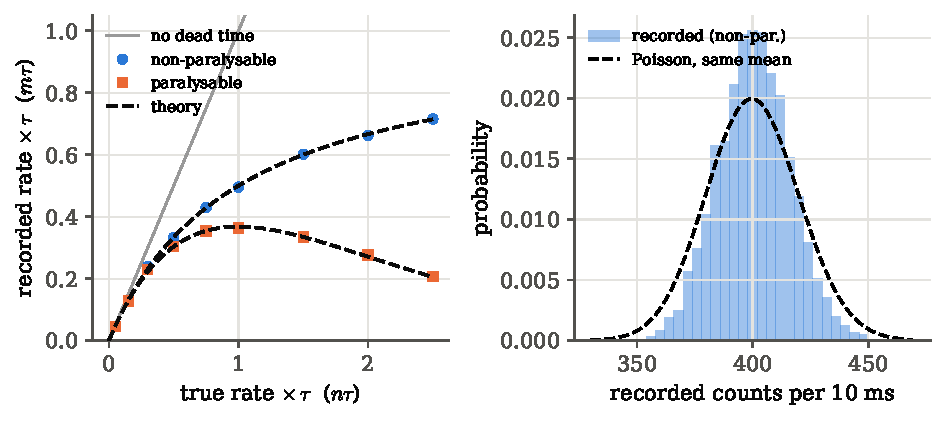
\includegraphics[width=\linewidth]{figures/ch02/08_deadtime.pdf}
\caption{Left: recorded rate against true rate, both in units of $1/\tau$. The simulated counters (dots and squares) sit on the derived curves $n\tau/(1+n\tau)$ and $n\tau e^{-n\tau}$ (dashed). The grey line is a perfect counter. The non-paralysable counter saturates at one hit per dead time; the paralysable one peaks at $n\tau=1$ and then falls. Right: the recorded counts per $10$~ms window at $n\tau=0.25$ (bars) form a visibly narrower histogram than a Poisson distribution with the same mean (dashed).}
\label{2a:fig:deadtime}
\end{figure}

The numbers it produced are these. The true hits give $\twoaDTRawMean$ counts per window on average (expected $\twoaDTTrueMean$) with $\hat F=\twoaDTRawFano$; by \eqref{2a:eq:fanosd} the Poisson scatter of $\hat F$ is $\twoaDTFanoSE$, so $\hat F-1$ is $\twoaDTRawPull$ times this scatter. The non-paralysable counter records a mean of $\twoaDTnpMean$ per window, against $\twoaDTnpTh$ from \eqref{2a:eq:dtnp}, and its Fano factor is $\twoaDTnpFano$, against $1/(1+n\tau)^2=\twoaDTnpFanoTh$. The paralysable counter records $\twoaDTpMean$ (theory $\twoaDTpTh$) with $\hat F=\twoaDTpFano$ (theory $1-2n\tau e^{-n\tau}=\twoaDTpFanoTh$). In units of their own scatter (for $F\ne1$ it is about $F\sqrt{2/(k-1)}$), the two dead-time Fano factors minus their predictions are $\twoaDTnpPull$ and $\twoaDTpPull$. The three numbers are not independent: all three come from the \emph{same} stream of true hits, so a chance fluctuation of that stream shows up in all three. Correcting the non-paralysable mean with \eqref{2a:eq:dtnp} gives $\hat n=\twoaDTnHat\times10^4~\text{s}^{-1}$ for the true rate of $5\times10^4~\text{s}^{-1}$, off by $\twoaDTnHatPull$ times its statistical error $\sqrt{n(1+n\tau)/T}\approx40~\text{s}^{-1}$ from \eqref{2a:eq:dtcorrvar}. The right panel of \cref{2a:fig:deadtime} is the underdispersion made visible.

\paragraph{How research uses it.} Here the simulation \emph{verified} formulas we had derived. Real detectors rarely match either idealised model: the dead time can depend on the pulse height, several stages of electronics can each have their own $\tau$, and afterpulsing adds clustering on top. For them the analytic route stops, and the same few lines of code become the instrument: simulate the true stream, pass it through a model of the electronics, and histogram the recorded counts. That histogram is the sampling distribution $P(S\given\theta)$ of the recorded count, and it goes into the likelihood (\cref{ch:03}). In a collider analysis, the Fano factor of event counts in stable running periods is a routine check that the luminosity and trigger were steady; in a survey, the excess over $F=1$ is the clustering signal itself.

\subsection{Large \texorpdfstring{$\lambda$}{lambda}: the Poisson count becomes Gaussian (a preview)}\label{2a:sec:gauss-preview}

In \cref{2a:fig:pois-limit} the Poisson pmf became more symmetric as $\lambda$ grew. For a large mean, a Poisson variable can be treated as a continuous Gaussian variable \srcref{Cowan}{\S2.2, p.~29}. Cumulants show why most quickly. The Poisson mgf is $M_X(t)=\exp[\lambda(e^t-1)]$, eq.~\eqref{2a:eq:poismgf}, so its cumulant generating function is
\begin{align}
  K_X(t)=\ln M_X(t) \eqby{1} \lambda(e^t-1) \eqby{2} \lambda\sum_{r=1}^\infty\frac{t^r}{r!}
  \quad\Longrightarrow\quad \kappa_r(X) \eqby{3} \lambda\quad\text{for every }r\ge1. \label{2a:eq:poiscum}
\end{align}
\begin{explain}
  \item Logarithm of the Poisson mgf.
  \item Taylor series of $e^t$ with the $r=0$ term cancelled by the $-1$.
  \item By definition the $r$-th cumulant $\kappa_r$ is $r!$ times the coefficient of $t^r$ in $K_X$. The first three cumulants are the mean, the variance and the third central moment.
\end{explain}
Now standardise, $Z=(X-\lambda)/\sqrt\lambda$. Since $K_{aX+b}(t)=bt+K_X(at)$, shifting by $b$ changes only $\kappa_1$ and scaling by $a$ multiplies $\kappa_r$ by $a^r$. With $a=1/\sqrt\lambda$,
\[
  \kappa_1(Z)=0,\qquad \kappa_2(Z)=1,\qquad \kappa_3(Z)=\frac{\lambda}{\lambda^{3/2}}=\frac1{\sqrt\lambda},\qquad \kappa_r(Z)=\lambda^{1-r/2}\xrightarrow{\;\lambda\to\infty\;}0\quad(r\ge3).
\]
So $K_Z(t)\to t^2/2$, which is the cumulant generating function of $\Normal(0,1)$: \emph{Poisson$(\lambda)$ is approximately $\Normal(\lambda,\lambda)$ for large $\lambda$}. The leading correction is the skewness $\kappa_3(Z)=1/\sqrt\lambda$, which shrinks only slowly: at $\lambda=25$ it is still $0.2$. The next part derives this limit properly (de Moivre--Laplace for the binomial, and the central limit theorem), with the corrections. It also explains why the limit holds. For integer $\lambda$, a Poisson$(\lambda)$ count is the sum of $\lambda$ independent Poisson$(1)$ counts, by the sum rule of \cref{2a:sec:poisson-process}, and sums of many independent terms tend to a Gaussian.

\begin{figure}[htbp]
\centering
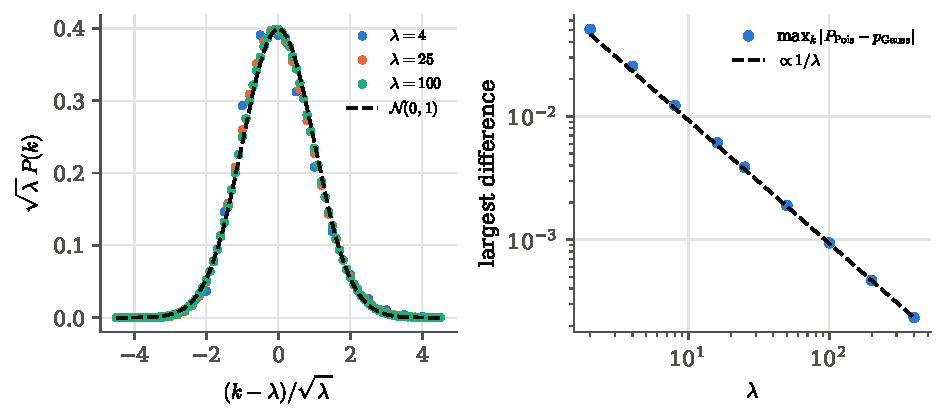
\includegraphics[width=\linewidth]{figures/ch02/08_poisson_gauss.pdf}
\caption{Left: Poisson pmfs for $\lambda=4$, $25$ and $100$, standardised so that the horizontal axis is the distance from the mean in standard deviations, and rescaled by $\sqrt\lambda$ so that they are comparable with a density. They crowd onto the standard Gaussian (dashed); at $\lambda=4$ the points are still lopsided, higher on the left of the peak and with a longer right tail. Right: the largest pointwise difference between the Poisson pmf and the Gaussian density falls like $1/\lambda$ (dashed line).}
\label{2a:fig:poisgauss}
\end{figure}

\Cref{2a:fig:poisgauss} shows the convergence. The largest difference $\max_k|P(k)-p_{\text{Gauss}}(k)|$ is $\twoaGaussDiffFour$ at $\lambda=4$, $\twoaGaussDiffTwentyfive$ at $\lambda=25$, $\twoaGaussDiffHundred$ at $\lambda=100$ and $\twoaGaussDiffFourHundred$ at $\lambda=400$. The $1/\lambda$ law has a simple reason: the peak height is about $1/\sqrt{2\pi\lambda}$, and the skewness correction to it is a fraction of order $\kappa_3(Z)=1/\sqrt\lambda$ of that height, so the absolute error is of order $1/\lambda$.

\paragraph{Example: a $4\sigma$ excess on a background of $25$.} A search region expects $b=25$ background events, with Poisson standard deviation $5$, and we observe $45$, which is $(45-25)/5=4$ standard deviations above the background. How often does background alone give $45$ or more? The Gaussian answer is $\Prob(Z\ge4)=\twoaTailGauss$. The exact Poisson answer, $\sum_{k\ge45}e^{-25}25^k/k!$, is $\twoaTailPois$: $\twoaTailRatio$ times larger. Even the \newterm{continuity correction} \unpack{treating the integer $45$ as the interval from $44.5$ up}, which gives $\twoaTailGaussCC$, is still wrong by a factor of four. Why so wrong? The Gaussian is good near the peak, where the $1/\lambda$ errors of \cref{2a:fig:poisgauss} are small in absolute terms. In the tail both probabilities are tiny, and a small absolute error is a large relative one. The Poisson right tail is heavier than the Gaussian one, because the Poisson is positively skewed. So the Gaussian \emph{understates} the chance of an upward fluctuation and overstates the significance of an excess. Tail probabilities, p-values and discovery claims (\cref{ch:04}) must use the exact Poisson distribution.

\subsection{Choosing a counting distribution}

Every counting distribution came from a mechanism, so recognising the mechanism is how we choose the distribution. The table collects them, with the Fano factor $F=\Var N/\E N$ as the quick check against data.

\begin{taxonomy}[which counting distribution, when]
\centering\small
\renewcommand{\arraystretch}{1.25}
\begin{tabular}{@{}>{\raggedright\arraybackslash}p{4.4cm}>{\raggedright\arraybackslash}p{2.7cm}>{\raggedright\arraybackslash}p{2.2cm}>{\raggedright\arraybackslash}p{2.1cm}@{}}
\textbf{mechanism} & \textbf{distribution} & \textbf{mean} & \textbf{Fano $F$}\\\hline
one yes/no trial & Bernoulli$(p)$ & $p$ & $1-p$\\
successes in $n$ independent trials, same $p$ & Binomial$(n,p)$ & $np$ & $1-p$\\
$N$ events sorted into bins, total fixed & Multinomial$(N,\bm p)$ & $Np_j$ per bin & $1-p_j$ per bin\\
many trials, rare successes; or a stream at constant rate with no memory & Poisson$(\lambda)$ & $\lambda$ & $1$\\
Poisson with a gamma-distributed rate, or clumped events & NegBin & $\mu$ & $1+\mu/\kappa$\\
counter blind for $\tau$ after each recorded hit & renewal count & $nT/(1+n\tau)$ & $(1+n\tau)^{-2}$\\
trials until the first / $r$-th success & Geometric / NegBin & $1/p$, $r/p$ & ---\\
time to the first / $n$-th event of a stream & Exponential / Gamma & $1/\lambda$, $n/\lambda$ & ---\\
\end{tabular}
\end{taxonomy}

The Fano column is the one to remember when data arrive. A value near $1$, judged against $\sqrt{2/(k-1)}$, supports a Poisson model. A value clearly above $1$ points to a fluctuating rate or clumping, and the negative binomial is the standard next model. A value clearly below $1$ points to dead time, pile-up rejection or a finite pool, and calls for a model of the detector. For large means the Poisson itself may be replaced by a Gaussian with variance equal to the mean, but only near the peak, never in the tails.

\begin{recap}[Part summary: counting distributions]
\begin{itemize}
  \item \textbf{Bernoulli} (one trial): $p^x(1-p)^{1-x}$, mean $p$, variance $p(1-p)$. Many independent trials give the product $p^z(1-p)^{N-z}$, which depends only on the number of successes.
  \item \textbf{Binomial} (successes in $n$ successive trials): count the $\binom nk$ paths, each of probability $p^k(1-p)^{n-k}$; mean $np$, variance $np(1-p)$; sums with the same $p$ stay binomial.
  \item \textbf{Multinomial} (histogram with fixed total): marginals binomial, covariance $-Np_ip_j$ between bins; with a Poisson total the bins become independent Poisson counts.
  \item \textbf{Poisson}: the $n\to\infty$, $np=\lambda$ limit of the binomial, and independently the count of a constant-rate, memoryless stream (from the ladder of differential equations $\dd P_n/\dd t=\lambda(P_{n-1}-P_n)$). Mean $=$ variance $=\lambda$. Closed under sums, thinning and binning.
  \item \textbf{Waiting times}: first event exponential (memoryless), $n$-th event Gamma$(n,1/\lambda)$ (Erlang); discrete versions geometric and negative binomial.
  \item \textbf{Failures}: a fluctuating rate or clumping gives $F>1$ (negative binomial); dead time gives $F<1$, with recorded rate $n/(1+n\tau)$ or $ne^{-n\tau}$ and $F=\sigma_I^2/m_I^2$ from the gaps; the dead-time correction removes the bias but inflates the variance by $1+n\tau$.
  \item \textbf{Large $\lambda$}: all Poisson cumulants equal $\lambda$, so the standardised count tends to $\Normal(0,1)$ with skewness $1/\sqrt\lambda$; use the exact Poisson in the tails.
\end{itemize}
\end{recap}
\providecommand{\tbStirTen}{}\renewcommand{\tbStirTen}{1.00837}
\providecommand{\tbStirOne}{}\renewcommand{\tbStirOne}{1.0844}
\providecommand{\tbDMLslope}{}\renewcommand{\tbDMLslope}{-1.00}
\providecommand{\tbDMLerrTen}{}\renewcommand{\tbDMLerrTen}{0.0168}
\providecommand{\tbDMLerrMax}{}\renewcommand{\tbDMLerrMax}{1.8\times10^{-5}}
\providecommand{\tbDMLnMax}{}\renewcommand{\tbDMLnMax}{10000}
\providecommand{\tbCBexact}{}\renewcommand{\tbCBexact}{0.268}
\providecommand{\tbCBplain}{}\renewcommand{\tbCBplain}{0.207}
\providecommand{\tbCBcc}{}\renewcommand{\tbCBcc}{0.270}
\providecommand{\tbCBsd}{}\renewcommand{\tbCBsd}{2.449}
\providecommand{\tbCLTskewOne}{}\renewcommand{\tbCLTskewOne}{2.01}
\providecommand{\tbCLTskewFive}{}\renewcommand{\tbCLTskewFive}{0.91}
\providecommand{\tbCLTskewThirty}{}\renewcommand{\tbCLTskewThirty}{0.366}
\providecommand{\tbCLTskewThirtyTh}{}\renewcommand{\tbCLTskewThirtyTh}{0.365}
\providecommand{\tbCLTslopeExp}{}\renewcommand{\tbCLTslopeExp}{-0.50}
\providecommand{\tbCLTslopeUni}{}\renewcommand{\tbCLTslopeUni}{-1.02}
\providecommand{\tbCLTDexpThirtyTwo}{}\renewcommand{\tbCLTDexpThirtyTwo}{0.0235}
\providecommand{\tbCLTDuniThirtyTwo}{}\renewcommand{\tbCLTDuniThirtyTwo}{8.7\times10^{-4}}
\providecommand{\tbCLTDexpOne}{}\renewcommand{\tbCLTDexpOne}{0.159}
\providecommand{\tbCLTBEthirty}{}\renewcommand{\tbCLTBEthirty}{3.64}
\providecommand{\tbCLTBEmodern}{}\renewcommand{\tbCLTBEmodern}{0.209}
\providecommand{\tbCLTDexpThirty}{}\renewcommand{\tbCLTDexpThirty}{0.0243}
\providecommand{\tbCLTrhothree}{}\renewcommand{\tbCLTrhothree}{2.415}
\providecommand{\tbCLTnsamp}{}\renewcommand{\tbCLTnsamp}{200000}
\providecommand{\tbBWgam}{}\renewcommand{\tbBWgam}{1.2476}
\providecommand{\tbBWiqrMean}{}\renewcommand{\tbBWiqrMean}{2.463}
\providecommand{\tbBWiqrTheory}{}\renewcommand{\tbBWiqrTheory}{2.495}
\providecommand{\tbBWnavg}{}\renewcommand{\tbBWnavg}{1000}
\providecommand{\tbBWfinalMean}{}\renewcommand{\tbBWfinalMean}{94.52}
\providecommand{\tbBWfinalOff}{}\renewcommand{\tbBWfinalOff}{3.3}
\providecommand{\tbBWfinalMedian}{}\renewcommand{\tbBWfinalMedian}{91.186}
\providecommand{\tbBWmedSE}{}\renewcommand{\tbBWmedSE}{0.0062}
\providecommand{\tbLanTailFrac}{}\renewcommand{\tbLanTailFrac}{6.1\times10^{-2}}
\providecommand{\tbLanTailGauss}{}\renewcommand{\tbLanTailGauss}{2.9\times10^{-7}}
\providecommand{\tbLanNlayers}{}\renewcommand{\tbLanNlayers}{25}
\providecommand{\tbMElam}{}\renewcommand{\tbMElam}{0.3710}
\providecommand{\tbMEpOne}{}\renewcommand{\tbMEpOne}{0.0544}
\providecommand{\tbMEpTwo}{}\renewcommand{\tbMEpTwo}{0.0788}
\providecommand{\tbMEpThree}{}\renewcommand{\tbMEpThree}{0.1142}
\providecommand{\tbMEpFour}{}\renewcommand{\tbMEpFour}{0.1654}
\providecommand{\tbMEpFive}{}\renewcommand{\tbMEpFive}{0.2398}
\providecommand{\tbMEpSix}{}\renewcommand{\tbMEpSix}{0.3475}
\providecommand{\tbMESmax}{}\renewcommand{\tbMESmax}{1.6136}
\providecommand{\tbMESrandMax}{}\renewcommand{\tbMESrandMax}{1.6139}
\providecommand{\tbMESrandMaxMean}{}\renewcommand{\tbMESrandMaxMean}{4.4966}
\providecommand{\tbMEminDeficit}{}\renewcommand{\tbMEminDeficit}{9.6\times10^{-4}}
\providecommand{\tbMEnKeep}{}\renewcommand{\tbMEnKeep}{7888}
\providecommand{\tbMESuniformDie}{}\renewcommand{\tbMESuniformDie}{1.7918}
\providecommand{\tbEntUniform}{}\renewcommand{\tbEntUniform}{1.2425}
\providecommand{\tbEntTriang}{}\renewcommand{\tbEntTriang}{1.3959}
\providecommand{\tbEntLaplace}{}\renewcommand{\tbEntLaplace}{1.3466}
\providecommand{\tbEntLogistic}{}\renewcommand{\tbEntLogistic}{1.4046}
\providecommand{\tbEntGauss}{}\renewcommand{\tbEntGauss}{1.4189}
\providecommand{\tbKangEnt}{}\renewcommand{\tbKangEnt}{0.1111}
\providecommand{\tbKangSq}{}\renewcommand{\tbKangSq}{0.0833}
\providecommand{\tbKangLog}{}\renewcommand{\tbKangLog}{0.1301}
\providecommand{\tbKangSqrt}{}\renewcommand{\tbKangSqrt}{0.1218}
\providecommand{\tbMVNfracOne}{}\renewcommand{\tbMVNfracOne}{0.6873}
\providecommand{\tbMVNfracTwo}{}\renewcommand{\tbMVNfracTwo}{0.9559}
\providecommand{\tbMVNlevOne}{}\renewcommand{\tbMVNlevOne}{2.296}
\providecommand{\tbMVNlevTwo}{}\renewcommand{\tbMVNlevTwo}{6.180}
\providecommand{\tbMVNcondMeanTh}{}\renewcommand{\tbMVNcondMeanTh}{3.600}
\providecommand{\tbMVNcondSdTh}{}\renewcommand{\tbMVNcondSdTh}{1.200}
\providecommand{\tbMVNcondMean}{}\renewcommand{\tbMVNcondMean}{3.614}
\providecommand{\tbMVNcondSd}{}\renewcommand{\tbMVNcondSd}{1.187}
\providecommand{\tbMVNnSlab}{}\renewcommand{\tbMVNnSlab}{9588}
\providecommand{\tbMVNmargSd}{}\renewcommand{\tbMVNmargSd}{1.997}
\providecommand{\tbMVNlamOne}{}\renewcommand{\tbMVNlamOne}{4.693}
\providecommand{\tbMVNlamTwo}{}\renewcommand{\tbMVNlamTwo}{0.307}
\providecommand{\tbMVNangle}{}\renewcommand{\tbMVNangle}{66.6}
\providecommand{\tbMVNN}{}\renewcommand{\tbMVNN}{20000}
\providecommand{\tbChiMeanFive}{}\renewcommand{\tbChiMeanFive}{5.010}
\providecommand{\tbChiVarFive}{}\renewcommand{\tbChiVarFive}{10.076}
\providecommand{\tbChiMeanTen}{}\renewcommand{\tbChiMeanTen}{9.993}
\providecommand{\tbChiVarTen}{}\renewcommand{\tbChiVarTen}{19.897}
\providecommand{\tbQFmean}{}\renewcommand{\tbQFmean}{2.999}
\providecommand{\tbQFvar}{}\renewcommand{\tbQFvar}{5.989}
\providecommand{\tbNaiveMean}{}\renewcommand{\tbNaiveMean}{2.997}
\providecommand{\tbNaiveVar}{}\renewcommand{\tbNaiveVar}{7.284}
\providecommand{\tbSVmeanS}{}\renewcommand{\tbSVmeanS}{4.0024}
\providecommand{\tbSVmeanSn}{}\renewcommand{\tbSVmeanSn}{3.2019}
\providecommand{\tbSVsigmaSq}{}\renewcommand{\tbSVsigmaSq}{4.0}
\providecommand{\tbSVbiasTh}{}\renewcommand{\tbSVbiasTh}{3.2000}
\providecommand{\tbSVwMean}{}\renewcommand{\tbSVwMean}{4.002}
\providecommand{\tbSVwVar}{}\renewcommand{\tbSVwVar}{8.022}
\providecommand{\tbSVcorrGauss}{}\renewcommand{\tbSVcorrGauss}{+0.0016}
\providecommand{\tbSVcorrExp}{}\renewcommand{\tbSVcorrExp}{+0.685}
\providecommand{\tbSVn}{}\renewcommand{\tbSVn}{5}
\providecommand{\tbSVnrep}{}\renewcommand{\tbSVnrep}{200000}
\providecommand{\tbTn}{}\renewcommand{\tbTn}{5}
\providecommand{\tbTdof}{}\renewcommand{\tbTdof}{4}
\providecommand{\tbTnrep}{}\renewcommand{\tbTnrep}{400000}
\providecommand{\tbTfracOneNineSix}{}\renewcommand{\tbTfracOneNineSix}{0.1209}
\providecommand{\tbTfracOneNineSixTh}{}\renewcommand{\tbTfracOneNineSixTh}{0.1216}
\providecommand{\tbZfracOneNineSix}{}\renewcommand{\tbZfracOneNineSix}{0.0497}
\providecommand{\tbTquant}{}\renewcommand{\tbTquant}{2.776}
\providecommand{\tbTfracQuant}{}\renewcommand{\tbTfracQuant}{0.0493}
\providecommand{\tbTfracThree}{}\renewcommand{\tbTfracThree}{0.0396}
\providecommand{\tbTfracThreeTh}{}\renewcommand{\tbTfracThreeTh}{0.0399}
\providecommand{\tbTfracThreeGauss}{}\renewcommand{\tbTfracThreeGauss}{0.0027}
\providecommand{\tbTmixNu}{}\renewcommand{\tbTmixNu}{3}
\providecommand{\tbTksMix}{}\renewcommand{\tbTksMix}{0.0010}
\providecommand{\tbTksUV}{}\renewcommand{\tbTksUV}{0.0013}
\providecommand{\tbFdOne}{}\renewcommand{\tbFdOne}{5}
\providecommand{\tbFdTwo}{}\renewcommand{\tbFdTwo}{10}
\providecommand{\tbFmean}{}\renewcommand{\tbFmean}{1.252}
\providecommand{\tbFmeanTh}{}\renewcommand{\tbFmeanTh}{1.250}
\providecommand{\tbFninetyfive}{}\renewcommand{\tbFninetyfive}{3.326}
\providecommand{\tbFfracNinetyfive}{}\renewcommand{\tbFfracNinetyfive}{0.0502}
\providecommand{\tbFksTsq}{}\renewcommand{\tbFksTsq}{0.0035}
\providecommand{\tbLNndyn}{}\renewcommand{\tbLNndyn}{10}
\providecommand{\tbLNmu}{}\renewcommand{\tbLNmu}{13.757}
\providecommand{\tbLNs}{}\renewcommand{\tbLNs}{0.4633}
\providecommand{\tbLNlnMean}{}\renewcommand{\tbLNlnMean}{13.758}
\providecommand{\tbLNlnSd}{}\renewcommand{\tbLNlnSd}{0.4629}
\providecommand{\tbLNmedian}{}\renewcommand{\tbLNmedian}{0.948}
\providecommand{\tbLNmedianTh}{}\renewcommand{\tbLNmedianTh}{0.943}
\providecommand{\tbLNmean}{}\renewcommand{\tbLNmean}{1.050}
\providecommand{\tbLNmeanTh}{}\renewcommand{\tbLNmeanTh}{1.050}
\providecommand{\tbLNmeanExact}{}\renewcommand{\tbLNmeanExact}{1.049}
\providecommand{\tbLNskew}{}\renewcommand{\tbLNskew}{1.333}
\providecommand{\tbLNskewLn}{}\renewcommand{\tbLNskewLn}{-0.054}
\providecommand{\tbMBsv}{}\renewcommand{\tbMBsv}{249.9}
\providecommand{\tbMBmean}{}\renewcommand{\tbMBmean}{398.9}
\providecommand{\tbMBmeanTh}{}\renewcommand{\tbMBmeanTh}{398.7}
\providecommand{\tbMBmodeTh}{}\renewcommand{\tbMBmodeTh}{353.4}
\providecommand{\tbMBrmsTh}{}\renewcommand{\tbMBrmsTh}{432.8}
\providecommand{\tbMBrms}{}\renewcommand{\tbMBrms}{432.8}
\providecommand{\tbRAYmean}{}\renewcommand{\tbRAYmean}{1.2531}
\providecommand{\tbRAYmeanTh}{}\renewcommand{\tbRAYmeanTh}{1.2533}
\providecommand{\tbPOWmean}{}\renewcommand{\tbPOWmean}{1.9986}
\providecommand{\tbPOWsd}{}\renewcommand{\tbPOWsd}{2.0012}
\providecommand{\tbOSn}{}\renewcommand{\tbOSn}{10}
\providecommand{\tbOSk}{}\renewcommand{\tbOSk}{3}
\providecommand{\tbOSmean}{}\renewcommand{\tbOSmean}{0.2728}
\providecommand{\tbOSmeanTh}{}\renewcommand{\tbOSmeanTh}{0.2727}
\providecommand{\tbOSvar}{}\renewcommand{\tbOSvar}{0.01659}
\providecommand{\tbOSvarTh}{}\renewcommand{\tbOSvarTh}{0.01653}
\providecommand{\tbGRmean}{}\renewcommand{\tbGRmean}{0.3846}
\providecommand{\tbGRmeanTh}{}\renewcommand{\tbGRmeanTh}{0.3846}
\providecommand{\tbRJacc}{}\renewcommand{\tbRJacc}{0.1123}
\providecommand{\tbRJaccTh}{}\renewcommand{\tbRJaccTh}{0.1119}
\providecommand{\tbRJkept}{}\renewcommand{\tbRJkept}{224548}
\providecommand{\tbRJmean}{}\renewcommand{\tbRJmean}{0.6428}
\providecommand{\tbRJmeanTh}{}\renewcommand{\tbRJmeanTh}{0.6429}
\providecommand{\tbRJsd}{}\renewcommand{\tbRJsd}{0.1240}
\providecommand{\tbRJsdTh}{}\renewcommand{\tbRJsdTh}{0.1237}
\providecommand{\tbDIRmeanOne}{}\renewcommand{\tbDIRmeanOne}{0.4999}
\providecommand{\tbDIRmeanOneTh}{}\renewcommand{\tbDIRmeanOneTh}{0.5000}
\providecommand{\tbDIRvarOne}{}\renewcommand{\tbDIRvarOne}{0.02767}
\providecommand{\tbDIRvarOneTh}{}\renewcommand{\tbDIRvarOneTh}{0.02778}
\providecommand{\tbDIRcov}{}\renewcommand{\tbDIRcov}{-0.01386}
\providecommand{\tbDIRcovTh}{}\renewcommand{\tbDIRcovTh}{-0.01389}
\providecommand{\tbWsig}{}\renewcommand{\tbWsig}{2.0}
\providecommand{\tbWDelta}{}\renewcommand{\tbWDelta}{10}
\providecommand{\tbWfwhm}{}\renewcommand{\tbWfwhm}{6.18}
\providecommand{\tbWsigEq}{}\renewcommand{\tbWsigEq}{2.63}
\providecommand{\tbWoutSim}{}\renewcommand{\tbWoutSim}{0.0820}
\providecommand{\tbWoutVoigt}{}\renewcommand{\tbWoutVoigt}{0.0825}
\providecommand{\tbWoutTail}{}\renewcommand{\tbWoutTail}{0.0794}
\providecommand{\tbWoutGauss}{}\renewcommand{\tbWoutGauss}{1.4\times10^{-4}}
\providecommand{\tbWrstar}{}\renewcommand{\tbWrstar}{3}
\providecommand{\tbWfaSim}{}\renewcommand{\tbWfaSim}{0.0112}
\providecommand{\tbWfaTh}{}\renewcommand{\tbWfaTh}{0.0111}
\providecommand{\tbWfaEight}{}\renewcommand{\tbWfaEight}{1.27\times10^{-14}}
\providecommand{\tbWpExact}{}\renewcommand{\tbWpExact}{0.0235}
\providecommand{\tbWzGauss}{}\renewcommand{\tbWzGauss}{2.12}
\providecommand{\tbWpGauss}{}\renewcommand{\tbWpGauss}{0.0169}
\providecommand{\tbWthreeGauss}{}\renewcommand{\tbWthreeGauss}{0.0027}
\providecommand{\tbWfiveGauss}{}\renewcommand{\tbWfiveGauss}{5.7\times10^{-7}}
\providecommand{\tbWthreeLap}{}\renewcommand{\tbWthreeLap}{0.0144}
\providecommand{\tbWfiveLap}{}\renewcommand{\tbWfiveLap}{8.5\times10^{-4}}
\providecommand{\tbWthreeTfive}{}\renewcommand{\tbWthreeTfive}{0.0117}
\providecommand{\tbWfiveTfive}{}\renewcommand{\tbWfiveTfive}{1.3\times10^{-3}}
\providecommand{\tbWthreeTthree}{}\renewcommand{\tbWthreeTthree}{0.0138}
\providecommand{\tbWfiveTthree}{}\renewcommand{\tbWfiveTthree}{3.2\times10^{-3}}
\providecommand{\tbWratioTthree}{}\renewcommand{\tbWratioTthree}{5650}
\section{The Gaussian, first way: the shape of a binomial with many trials}
\label{2b:sec:gauss-binomial}

The same bell-shaped curve describes a calorimeter energy, a timing residual, a CMB temperature and a strain sample. None of these is a count: the counting distributions of the first half of the chapter live on the integers, and these quantities do not. There are three separate routes to the bell curve, and each route tells us \emph{when} to trust it. The oldest route starts from a count after all. Take a binomial distribution with a very large number of trials and ask what shape it takes.

\paragraph{Ten thousand photo-electrons.}
A scintillator bar is hit by a cosmic muon. It produces $n=10\,000$ photons, and each photon independently reaches the photomultiplier and makes a photo-electron with probability $p=0.3$. The number of photo-electrons $k$ is Binomial$(n,p)$ (see the counting part of this chapter). To compute $\Prob(k\le 2950)$ exactly we would add $2951$ terms, each containing factorials of numbers near $10^4$. Nobody does that. Instead everyone replaces the binomial by a smooth bell curve with mean $np=3000$ and standard deviation $\sqrt{np(1-p)}\approx 45.8$.

That replacement raises four questions. Which bell curve, exactly? Why a bell and not some other shape? How large must $n$ be? And how do we correct for the fact that $k$ is an integer while the curve is smooth? The large-$n$ limit of the binomial answers all four.

\paragraph{Zooming in on the peak of a mountain.}
The Gaussian is what \emph{every} smooth, single-peaked, sharply concentrated distribution looks like near its maximum. Here is why. For large $n$ the binomial pmf is a tall, narrow mountain centred at $np$, and its width grows only like $\sqrt n$. Plot the \emph{logarithm} of any smooth mountain: near its summit it looks like a downward parabola. The exponential of a parabola is a Gaussian. This is the same move as the harmonic approximation in mechanics: expand the potential to second order about its minimum and the motion becomes simple harmonic. Here we expand $\ln\Prob(k)$ to second order about its maximum.

\paragraph{The plan.}
\begin{enumerate}[label=\arabic*.]
  \item Which quantity do we want? The probability of $k$ successes in $n$ trials when $n$ is large.
  \item What makes it hard? Factorials of large numbers. So first find a good formula for $n!$ (Stirling).
  \item Where is the probability concentrated? Near $k=np$, in a window of width $\sqrt{np(1-p)}$.
  \item What does $\ln\Prob(k)$ look like in that window? Expand it in powers of the distance from the peak and keep what survives as $n\to\infty$.
  \item How do we turn a statement about integers into one about a continuous variable, and what does that cost? (The continuity correction.)
\end{enumerate}

\subsection{The Gaussian density and what its two parameters do}
\label{2b:sec:gauss-def}

\begin{workdef}[Gaussian (normal) distribution]
A continuous random variable $X$ has a \newterm{Gaussian} or \newterm{normal} distribution with parameters $\mu$ and $\sigma^2$, written $X\sim\Normal(\mu,\sigma^2)$, if its density \unpack{probability per unit $x$, so it has units of $1/x$} is
\begin{equation}
  p(x\given\mu,\sigma^2)=\frac{1}{\sqrt{2\pi\sigma^2}}\exp\!\left[-\frac{(x-\mu)^2}{2\sigma^2}\right],\qquad -\infty<x<\infty ,
  \label{2b:eq:gauss}
\end{equation}
with $\mu\in\R$ and $\sigma>0$. The case $\mu=0$, $\sigma=1$ is the \newterm{standard normal} $Z\sim\Normal(0,1)$, with density $\varphi(z)=e^{-z^2/2}/\sqrt{2\pi}$ and cumulative distribution function \unpack{the probability of landing at or below $z$} $\Phi(z)=\int_{-\infty}^z\varphi(z')\,\dd z'$.
\emph{Operational test:} standardise, $z=(x-\mu)/\sigma$, and compare the histogram of $z$ with $\varphi$ (or the ordered $z$ values with the quantiles $\Phi^{-1}$).
\end{workdef}

Three facts make the Gaussian usable. We check each one.

\paragraph{It is normalised.} The function $e^{-z^2/2}$ has no elementary antiderivative, so the normalisation needs a trick: square the integral and go to polar coordinates \srcref{CasellaBerger}{p.~84--85}. Let $I=\int_{-\infty}^{\infty}e^{-z^2/2}\dd z$. Then
\begin{align}
  I^2
  &\eqby{1} \int_{-\infty}^{\infty}\!\!\int_{-\infty}^{\infty} e^{-(u^2+v^2)/2}\,\dd u\,\dd v \nonumber\\
  &\eqby{2} \int_{0}^{2\pi}\!\!\int_{0}^{\infty} e^{-r^2/2}\,r\,\dd r\,\dd\phi \nonumber\\
  &\eqby{3} 2\pi\Bigl[-e^{-r^2/2}\Bigr]_0^{\infty} \nonumber\\
  &= 2\pi .
  \label{2b:eq:gauss-integral}
\end{align}
\begin{explain}
  \item The two copies of the integral use independent dummy variables $u$ and $v$, and a product of two integrals is a double integral over the plane.
  \item Polar coordinates $u=r\cos\phi$, $v=r\sin\phi$: then $u^2+v^2=r^2$ and the area element is $\dd u\,\dd v=r\,\dd r\,\dd\phi$.
  \item The $\phi$ integral gives $2\pi$. The extra factor $r$ makes the $r$ integral elementary, since $\frac{\dd}{\dd r}\bigl(-e^{-r^2/2}\bigr)=r\,e^{-r^2/2}$.
\end{explain}
So $I=\sqrt{2\pi}$, which is the constant in $\varphi$. Substituting $z=(x-\mu)/\sigma$, $\dd x=\sigma\,\dd z$, gives the constant $1/\sqrt{2\pi\sigma^2}$ in \eqref{2b:eq:gauss}. A by-product: with $w=z^2/2$ the half-line integral becomes $\int_0^\infty w^{-1/2}e^{-w}\dd w=\Gamma(\tfrac12)$, so
\begin{equation}
  \Gamma(\tfrac12)=\sqrt\pi ,
  \label{2b:eq:gamma-half}
\end{equation}
where $\Gamma(\alpha)=\int_0^\infty t^{\alpha-1}e^{-t}\dd t$ is the Gamma function, with $\Gamma(\alpha+1)=\alpha\Gamma(\alpha)$ (integrate by parts) and $\Gamma(n+1)=n!$ for integers. We need all three facts for $\chi^2$ later.

\paragraph{$\mu$ is the mean and $\sigma^2$ the variance.} With $x=\mu+\sigma z$,
\begin{align}
  \E(X)
  &\eqby{1} \mu+\sigma\int_{-\infty}^{\infty} z\,\varphi(z)\,\dd z \eqby{2} \mu , \nonumber\\
  \Var(X)
  &\eqby{3} \sigma^2\int_{-\infty}^{\infty} z^2\varphi(z)\,\dd z
   \eqby{4} \sigma^2\Bigl\{\bigl[-z\varphi(z)\bigr]_{-\infty}^{\infty}+\int_{-\infty}^{\infty}\varphi(z)\,\dd z\Bigr\}
   \eqby{5} \sigma^2 .
  \label{2b:eq:gauss-moments}
\end{align}
\begin{explain}
  \item Change variables and use $\int\varphi=1$ for the constant term.
  \item The integrand $z\varphi(z)$ is odd, so the integral over a symmetric range vanishes.
  \item $\Var(X)=\E(X-\mu)^2$ and $(x-\mu)^2=\sigma^2z^2$.
  \item Integrate by parts with $u=z$ and $\dd v=z\varphi(z)\dd z$, whose integral is $v=-\varphi(z)$ because $\varphi'(z)=-z\varphi(z)$.
  \item The boundary term vanishes because $\varphi$ decays faster than any power, and the remaining integral is $1$.
\end{explain}
So the two parameters are exactly the mean and the variance \srcref{Cowan}{(2.23)--(2.24)}. This is special: for most distributions the parameters are \emph{not} the mean and variance (the log-normal of \cref{2b:sec:zoo} is a warning example).

\paragraph{Standardising reduces everything to one table.} If $X\sim\Normal(\mu,\sigma^2)$ then $Z=(X-\mu)/\sigma\sim\Normal(0,1)$ and, conversely, $X=\mu+\sigma Z$ \mainref{p.~28}. Hence
\begin{equation}
  \Prob(a<X<b)=\Phi\!\left(\frac{b-\mu}{\sigma}\right)-\Phi\!\left(\frac{a-\mu}{\sigma}\right).
  \label{2b:eq:gauss-prob}
\end{equation}
Two numbers are worth knowing by heart. First, the probability within $1$, $2$, $3$ standard deviations of the mean is $0.6827$, $0.9545$, $0.9973$ (\cref{2b:fig:gauss-bands}). Second, ``one sigma'' can be read off a plot by eye: it is where the curve stops bending down and starts bending up. To see this, note that the density has its maximum at $x=\mu$, and its second derivative $\varphi''(z)=(z^2-1)\varphi(z)$ vanishes at $z=\pm1$. So the inflection points sit at $x=\mu\pm\sigma$.

\begin{figure}[htbp]
\centering
\begin{tikzpicture}
\begin{axis}[width=11cm,height=5.2cm,domain=-4:4,samples=161,
  axis lines=left,xlabel={$z=(x-\mu)/\sigma$},ylabel={$\varphi(z)$},
  ymin=0,ymax=0.47,xtick={-3,-2,-1,0,1,2,3},ytick={0,0.1,0.2,0.3,0.4},
  every axis plot/.append style={thick}]
  \addplot[draw=none,fill=formblue!10,domain=-3:3] {exp(-x^2/2)/sqrt(2*pi)} \closedcycle;
  \addplot[draw=none,fill=formblue!22,domain=-2:2] {exp(-x^2/2)/sqrt(2*pi)} \closedcycle;
  \addplot[draw=none,fill=formblue!40,domain=-1:1] {exp(-x^2/2)/sqrt(2*pi)} \closedcycle;
  \addplot[formblue] {exp(-x^2/2)/sqrt(2*pi)};
  \addplot[only marks,mark=*,mark size=1.6pt,bdryred] coordinates {(-1,0.2420) (1,0.2420)};
  \node[font=\scriptsize,anchor=east,bdryred] at (axis cs:-1.05,0.262) {inflection};
  \node[font=\scriptsize] at (axis cs:0,0.12) {$68.3\%$};
  \node[font=\scriptsize] at (axis cs:1.5,0.035) {$95.4\%$};
  \node[font=\scriptsize] at (axis cs:3.35,0.045) {$99.7\%$};
  \draw[faint] (axis cs:2.55,0.012) -- (axis cs:3.15,0.038);
\end{axis}
\end{tikzpicture}
\caption{The standard normal density. The darkest band ($|z|<1$) holds $68.3\%$ of the probability, the band out to $|z|<2$ holds $95.4\%$, and out to $|z|<3$ holds $99.7\%$. The red dots are the inflection points at $z=\pm1$: one standard deviation is where the curve changes from bending down to bending up.}
\label{2b:fig:gauss-bands}
\end{figure}

\paragraph{Example: Reading the table both ways.}
\label{2b:ex:aos-gauss}
Let $X\sim\Normal(3,5)$. The second argument is the \emph{variance}, so $\sigma=\sqrt5$. A table of $\Phi$ answers two kinds of question. The forward question gives a cut and asks for a probability: what is $\Prob(X>1)$?
\begin{align*}
  \Prob(X>1)
  &\eqby{1} 1-\Prob(X<1)
  \eqby{2} 1-\Phi\!\left(\frac{1-3}{\sqrt5}\right)
  = 1-\Phi(-0.8944)
  \eqby{3} 0.81 .
\end{align*}
\begin{explain}
  \item Complement rule. For a continuous variable $\Prob(X=1)=0$, so $<$ and $\le$ do not matter.
  \item Standardise with \eqref{2b:eq:gauss-prob}.
  \item From a table or \pyname{scipy.stats.norm.cdf}: $\Phi(-0.8944)=0.1855$.
\end{explain}
The quantile question goes the other way. It gives a probability and asks for the cut: which $q$ has $\Prob(X<q)=0.2$?
\begin{align*}
  0.2=\Prob(X<q)
  &\eqby{1} \Phi\!\left(\frac{q-3}{\sqrt5}\right)
  \;\Longrightarrow\; \frac{q-3}{\sqrt5}\eqby{2}\Phi^{-1}(0.2)=-0.8416 \\
  &\;\Longrightarrow\; q\eqby{3}3-0.8416\sqrt5=1.1181 .
\end{align*}
\begin{explain}
  \item Standardise.
  \item $\Phi$ is strictly increasing, so it can be inverted. $\Phi^{-1}$ is \pyname{scipy.stats.norm.ppf}.
  \item Solve the linear equation for $q$.
\end{explain}
These are the two numbers of \mainref{p.~29, Example~2.17}.

\begin{pitfall}[$\Normal(\mu,\sigma^2)$ or $\Normal(\mu,\sigma)$?]
AoS, Cowan and CasellaBerger write the \emph{variance} as the second argument. Lambert and most software (\pyname{scipy.stats.norm(loc, scale)}, \pyname{numpy.random.normal(loc, scale)}) take the \emph{standard deviation}. $\Normal(3,5)$ in AoS is \pyname{norm(3, sqrt(5))} in scipy. Always check which one a formula or a function expects.
\end{pitfall}

\subsection{Stirling's formula from Laplace's method}
\label{2b:sec:stirling}

The binomial is built from factorials, so we need a good formula for $n!$ when $n$ is large. That formula is Stirling's:
\begin{equation}
  n! \simeq \sqrt{2\pi n}\;n^n e^{-n}\qquad (n\to\infty),
  \qquad\text{i.e.}\qquad
  \ln n! = n\ln n-n+\tfrac12\ln(2\pi n)+O(1/n) .
  \label{2b:eq:stirling}
\end{equation}

It comes from the same zoom-in on a peak, now applied to an integral. \emph{The starting point.} The Gamma function gives $n!$ as an integral, $n!=\Gamma(n+1)=\int_0^\infty t^n e^{-t}\dd t$, and for large $n$ its integrand is sharply peaked. \emph{Where is the peak, and how sharp is it?} Write the integrand as $e^{f(t)}$ with $f(t)=n\ln t-t$. The slope $f'(t)=n/t-1$ vanishes at $t=n$, so the peak is at $t=n$. The curvature $f''(t)=-n/t^2$ equals $-1/n$ there. \emph{Only then the integral.} Expanding $f$ to second order about its maximum,
\begin{align}
  n!
  &\eqby{1} \int_0^\infty \exp\Bigl[f(n)+f'(n)(t-n)+\tfrac12 f''(n)(t-n)^2+\dots\Bigr]\dd t \nonumber\\
  &\eqby{2} n^n e^{-n}\int_0^\infty \exp\Bigl[-\frac{(t-n)^2}{2n}+\dots\Bigr]\dd t \nonumber\\
  &\eqby{3} n^n e^{-n}\int_{-\infty}^{\infty} e^{-s^2/(2n)}\dd s\;\bigl(1+O(1/n)\bigr) \nonumber\\
  &\eqby{4} \sqrt{2\pi n}\;n^n e^{-n}\bigl(1+O(1/n)\bigr) .
  \label{2b:eq:stirling-derivation}
\end{align}
\begin{explain}
  \item Taylor expansion of $f$ about $t=n$ inside the exponential.
  \item $f(n)=n\ln n-n$ gives $e^{f(n)}=n^ne^{-n}$, the linear term vanishes because $t=n$ is the maximum, and $\tfrac12f''(n)=-1/(2n)$.
  \item Substitute $s=t-n$. The integrand is negligible beyond a few multiples of $\sqrt n$ from the peak, so extending the lower limit from $s=-n$ to $-\infty$ adds only a Gaussian tail of order $e^{-n/2}$. The cubic and higher terms of the expansion give the relative correction of order $1/n$ (it is $1/(12n)$).
  \item The Gaussian integral \eqref{2b:eq:gauss-integral} with $\sigma^2=n$.
\end{explain}
This is \newterm{Laplace's method}: a sharply peaked integrand $e^{f(t)}$ is replaced by a Gaussian with the same peak height and the same curvature. We will meet it again as the Gaussian (Laplace) approximation to a posterior in \cref{ch:05}. \Cref{2b:fig:laplace} shows how good the approximation already is at $n=10$.

\begin{figure}[htbp]
\centering
\begin{tikzpicture}
\begin{axis}[width=11cm,height=5cm,domain=0.05:30,samples=200,
  axis lines=left,xlabel={$t$},ylabel={integrand$/$peak},
  ymin=0,ymax=1.15,xmin=0,xmax=30,legend cell align=left,legend style={draw=none,font=\scriptsize,at={(0.98,0.95)},anchor=north east},
  every axis plot/.append style={thick}]
  \addplot[formblue] {exp(10*ln(x/10)-(x-10))};
  \addlegendentry{integrand $t^{10}e^{-t}$, scaled}
  \addplot[black,dashed] {exp(-(x-10)^2/20)};
  \addlegendentry{Gaussian}
  \draw[tangentgreen,<->] (axis cs:10-3.1623,0.6065) -- (axis cs:10+3.1623,0.6065);
  \node[font=\scriptsize,tangentgreen,anchor=south] at (axis cs:10,0.66) {$2\sqrt{n}$};
\end{axis}
\end{tikzpicture}
\caption{Laplace's method for $10!=\int_0^\infty t^{10}e^{-t}\dd t$. The integrand (blue) is scaled to peak height one at $t=n=10$. The dashed Gaussian has the same peak and the same curvature there, so its width is $\sqrt n$. The two areas differ by less than one percent, and the mismatch is the slight skew of the blue curve, which the $1/(12n)$ correction describes.}
\label{2b:fig:laplace}
\end{figure}

Stirling's formula is accurate even for small $n$. The script below finds $n!/\text{Stirling}=\tbStirOne$ at $n=1$ and $\tbStirTen$ at $n=10$, in agreement with $1+1/(12n)$ (\cref{2b:fig:demoivre-errors}a). Even $1!$ is off by only eight percent.

\subsection{The de Moivre--Laplace limit}
\label{2b:sec:demoivre}

\begin{keyidea}[de Moivre--Laplace]
Let $k\sim\text{Binomial}(n,p)$ and $q=1-p$. For large $n$ and $k$ within a few $\sqrt{npq}$ of $np$,
\begin{equation}
  \Prob(k)=\binom nk p^kq^{n-k}\simeq \frac{1}{\sqrt{2\pi npq}}\exp\!\left[-\frac{(k-np)^2}{2npq}\right].
  \label{2b:eq:dml}
\end{equation}
The binomial pmf becomes a Gaussian density with $\mu=np$ and $\sigma^2=npq$, the binomial mean and variance.
\end{keyidea}

The derivation takes two steps. First, replace each factorial by Stirling's formula. Second, Taylor-expand the exponent about the peak. \emph{Step one.} Insert \eqref{2b:eq:stirling} for $n!$, $k!$ and $(n-k)!$:
\begin{align}
  \ln\Prob(k)
  &\eqby{1} \ln n!-\ln k!-\ln(n-k)!+k\ln p+(n-k)\ln q \nonumber\\
  &\eqby{2} \bigl[n\ln n-k\ln k-(n-k)\ln(n-k)+k\ln p+(n-k)\ln q\bigr]
     -\tfrac12\ln\frac{2\pi k(n-k)}{n} \nonumber\\
  &\eqby{3} -k\ln\frac{k}{np}-(n-k)\ln\frac{n-k}{nq}-\tfrac12\ln\frac{2\pi k(n-k)}{n} .
  \label{2b:eq:dml-step1}
\end{align}
\begin{explain}
  \item The logarithm of the binomial pmf.
  \item Stirling for the three factorials. The $-n+k+(n-k)$ from the three ``$-m$'' terms cancels. The three $\tfrac12\ln(2\pi m)$ terms combine into the last logarithm.
  \item Write $n\ln n=k\ln n+(n-k)\ln n$ and collect: $k\ln n-k\ln k+k\ln p=-k\ln\frac{k}{np}$, and the same for the $n-k$ terms.
\end{explain}
\emph{Step two.} Measure $k$ from the centre of the binomial, $k=np+\delta$, so that $\delta$ is the distance from the peak. Then $n-k=nq-\delta$, $k/(np)=1+\delta/(np)$ and $(n-k)/(nq)=1-\delta/(nq)$. Each logarithm in \eqref{2b:eq:dml-step1} now has the form $\ln(1+x)$ with $x$ small, so we use $\ln(1+x)=x-\tfrac{x^2}{2}+\tfrac{x^3}{3}-\dots$:
\begin{align}
  (np+\delta)\ln\Bigl(1+\frac{\delta}{np}\Bigr)
  &\eqby{1} (np+\delta)\Bigl(\frac{\delta}{np}-\frac{\delta^2}{2n^2p^2}+\frac{\delta^3}{3n^3p^3}\Bigr)+O\Bigl(\frac{\delta^4}{n^3}\Bigr) \nonumber\\
  &\eqby{2} \delta+\frac{\delta^2}{2np}-\frac{\delta^3}{6n^2p^2}+O\Bigl(\frac{\delta^4}{n^3}\Bigr),\nonumber\\
  (nq-\delta)\ln\Bigl(1-\frac{\delta}{nq}\Bigr)
  &\eqby{3} -\delta+\frac{\delta^2}{2nq}+\frac{\delta^3}{6n^2q^2}+O\Bigl(\frac{\delta^4}{n^3}\Bigr) .
  \label{2b:eq:dml-taylor}
\end{align}
\begin{explain}
  \item Taylor series of the logarithm to third order.
  \item Multiply out: $\delta^2$ terms $\frac{\delta^2}{np}-\frac{\delta^2}{2np}=\frac{\delta^2}{2np}$, and $\delta^3$ terms $-\frac{\delta^3}{2n^2p^2}+\frac{\delta^3}{3n^2p^2}=-\frac{\delta^3}{6n^2p^2}$.
  \item The same calculation with $p\to q$ and $\delta\to-\delta$.
\end{explain}
The exponent in \eqref{2b:eq:dml-step1} is minus the sum of these two lines:
\begin{align}
  -k\ln\frac{k}{np}-(n-k)\ln\frac{n-k}{nq}
  &\eqby{1} -\frac{\delta^2}{2n}\Bigl(\frac1p+\frac1q\Bigr)+\frac{\delta^3}{6n^2}\Bigl(\frac1{p^2}-\frac1{q^2}\Bigr)+\dots \nonumber\\
  &\eqby{2} -\frac{\delta^2}{2npq}+\frac{\delta^3}{6n^2}\,\frac{q^2-p^2}{p^2q^2}+\dots
  \label{2b:eq:dml-exponent}
\end{align}
\begin{explain}
  \item The $\pm\delta$ terms cancel. This cancellation is what puts the peak at $np$.
  \item $\frac1p+\frac1q=\frac{p+q}{pq}=\frac1{pq}$ because $p+q=1$.
\end{explain}
\emph{Which terms survive?} Only the quadratic one. The probability sits where $\delta$ is of order $\sqrt{npq}$, so we judge each term there. The quadratic term $\delta^2/(2npq)$ is of order $1$. The cubic term is of order $n^{3/2}/n^2=n^{-1/2}$, which goes to zero. The prefactor also simplifies: $k(n-k)/n=npq+\delta(q-p)-\delta^2/n=npq\,[1+O(n^{-1/2})]$. Dropping the terms that vanish gives \eqref{2b:eq:dml}.

The cubic term also says how fast the limit is reached, in two ways. For $p=q=\tfrac12$ it is exactly zero, so the symmetric binomial converges faster. And the leading corrections are \emph{odd} in $\delta$: they skew the curve but leave its height at the peak unchanged. So the largest pointwise error is the relative correction $n^{-1/2}$ times the height of the pmf, also of order $n^{-1/2}$, which gives $n^{-1}$.

\begin{pitfall}[The approximation is local]
\eqref{2b:eq:dml} was derived for $\delta=O(\sqrt n)$. Far in the tails, say $\delta\sim n$, the neglected cubic and higher terms are \emph{not} small and the relative error can be enormous, even though both probabilities are tiny. A ``$5\sigma$'' tail probability computed from the Gaussian approximation to a binomial or Poisson count can be off by a large factor. For tail probabilities use the exact distribution (\pyname{scipy.stats.binom.sf}).
\end{pitfall}

\paragraph{Example: The continuity correction.}
\label{2b:ex:continuity}
An integer count has to be matched to a smooth curve, and the match is best when we cut half-way between integers. Let $X\sim\text{Binomial}(25,0.6)$, so $\mu=15$ and $\sigma=\sqrt{25\cdot0.6\cdot0.4}=\tbCBsd$. We want $\Prob(X\le13)$. Think of each integer $k$ as a bar of width one centred on $k$, so the bar for $k=13$ reaches up to $13.5$. The plain Gaussian approximation cuts at $13$ and misses half of that bar. The \newterm{continuity correction} cuts at $13.5$ instead:
\begin{align*}
  \Prob(X\le13)
  &\eqby{1} \Prob(X\le13.5)
  \eqby{2} \Phi\!\left(\frac{13.5-15}{\tbCBsd}\right)
  = \tbCBcc .
\end{align*}
\begin{explain}
  \item $X$ is an integer, so $X\le13$ and $X\le13.5$ are the same event. The bar picture tells us to use the second when replacing the pmf by a density.
  \item de Moivre--Laplace with $\mu=np$, $\sigma^2=npq$, then standardise.
\end{explain}
The exact binomial sum is $\tbCBexact$ and the uncorrected approximation $\Phi\bigl((13-15)/\tbCBsd\bigr)=\tbCBplain$. The half-bar is worth six percentage points here. In general, $\Prob(X\le x)\approx\Phi\bigl((x+\tfrac12-\mu)/\sigma\bigr)$ and $\Prob(X\ge x)\approx1-\Phi\bigl((x-\tfrac12-\mu)/\sigma\bigr)$.

\paragraph{Example: How many photo-electrons?}
Back to the scintillator bar of the opening: $n=10^4$ photons, each making a photo-electron with probability $p=0.3$, so $\mu=np=3000$ and $\sigma=\sqrt{npq}=\sqrt{2100}=45.83$. We wanted $\Prob(k\le2950)$:
\begin{align*}
  \Prob(k\le2950)
  &\eqby{1}\Phi\!\left(\frac{2950.5-3000}{45.83}\right)
  =\Phi(-1.080)
  \eqby{2}0.140 .
\end{align*}
\begin{explain}
  \item de Moivre--Laplace with the continuity correction.
  \item Table value. The exact binomial sum (\pyname{binom.cdf(2950, 10000, 0.3)}) agrees to three decimal places.
\end{explain}
The same numbers give the bar's energy resolution. The relative width $\sigma/\mu=\sqrt{q/(np)}=1.5\%$ is its photo-statistics term. It falls like $1/\sqrt{\text{number of photo-electrons}}$, the famous $a/\sqrt E$ term of calorimetry.

\paragraph{Exercise: when is $n$ large enough.}
CasellaBerger's rule of thumb is $\min(np,\,nq)\ge5$ \srcref{CasellaBerger}{p.~85}. Use \eqref{2b:eq:dml-exponent} to explain why the rule involves the \emph{smaller} of $np$ and $nq$. (Answer: the relative size of the cubic term at $\delta=\sigma$ is $\frac{\sigma^3}{6n^2}\frac{|q^2-p^2|}{p^2q^2}=\frac{|q-p|}{6\sqrt{npq}}$, which is large when either $np$ or $nq$ is small, i.e.\ when the distribution is squeezed against $k=0$ or $k=n$.)

\subsection{Python: watching the binomial become a Gaussian}
\label{2b:sec:dml-python}

The script computes Stirling's ratio, overlays the Gaussian on three binomials, and measures the largest pointwise error as $n$ grows from $10$ to $10^4$. The first key lines check Stirling's formula:

\pyfile[firstline=29,lastline=33,firstnumber=29]{code/ch02/20_demoivre_laplace.py}{Stirling's formula against the exact $\ln n!$}

Line 31 uses \pyname{gammaln}, the logarithm of the Gamma function, because $n!$ itself overflows a double for $n>170$. Any likelihood code works with logarithms of factorials for the same reason. The next lines measure how far the binomial is from its Gaussian:

\pyfile[firstline=54,lastline=62,firstnumber=54]{code/ch02/20_demoivre_laplace.py}{The largest error of the de Moivre--Laplace approximation}

For each $n$ on a logarithmic grid, line 60 compares the exact pmf with the Gaussian density at the same integers and keeps the worst case. Line 62 fits a straight line in log--log space. The slope comes out as $\tbDMLslope$, the $n^{-1}$ predicted above from the odd (skewing) corrections. At $n=10$ the largest error is $\tbDMLerrTen$, at $n=\tbDMLnMax$ it is $\tbDMLerrMax$ (\cref{2b:fig:demoivre-errors}b).

\begin{figure}[htbp]
\centering
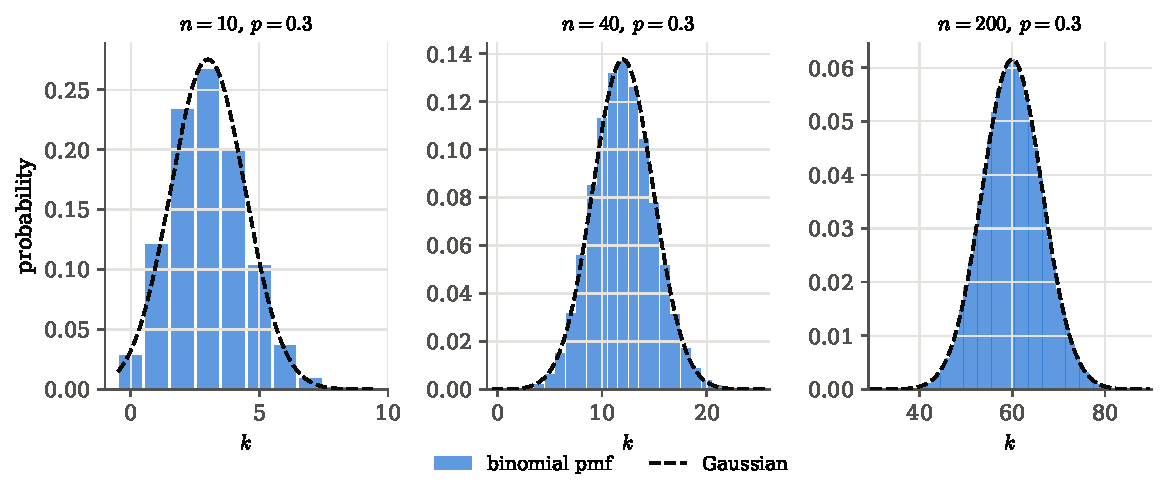
\includegraphics[width=\linewidth]{figures/ch02/demoivre_panels.pdf}
\caption{Binomial$(n,0.3)$ probabilities (bars) with the Gaussian of the same mean and variance (dashed) for $n=10$, $40$, $200$. At $n=10$ the bars lean to the right of the curve: the distribution is squeezed against $k=0$ and is skewed. By $n=200$ the skew is invisible by eye.}
\label{2b:fig:demoivre-panels}
\end{figure}

\begin{figure}[htbp]
\centering
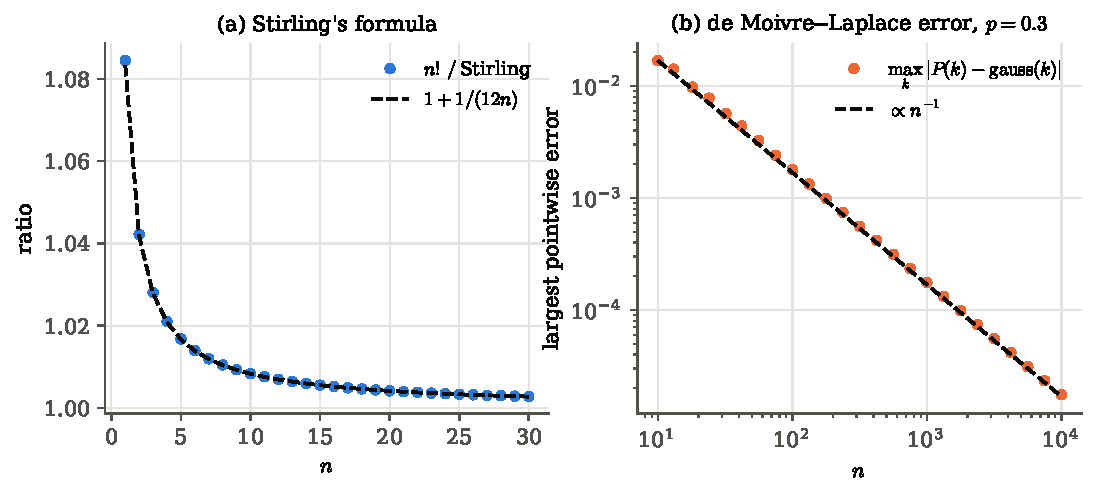
\includegraphics[width=\linewidth]{figures/ch02/demoivre_errors.pdf}
\caption{(a) The ratio of the exact $n!$ to Stirling's formula approaches one from above, following $1+1/(12n)$. (b) The largest pointwise difference between the binomial pmf and its Gaussian approximation falls as $1/n$ (dashed line).}
\label{2b:fig:demoivre-errors}
\end{figure}

\paragraph{What this bought us.}
The Gaussian appears whenever a distribution is sharply peaked and we look on the scale of its width: the logarithm is a parabola there. For the binomial the parabola has curvature $1/(npq)$, which fixes the Gaussian completely. The first correction is a skew of relative size $|q-p|/\sqrt{npq}$, and it is the skew, not the width, that tells us whether $n$ is large enough.

\begin{inpractice}[Verifying a limit versus relying on it]
Here the plot only \emph{verifies} a known limit: the exact pmf is cheap, so nothing hangs on the approximation. Research uses the same Gaussian replacement where no exact answer is at hand. A binned $\chi^2$ fit to a histogram treats each bin count, a binomial or Poisson number, as Gaussian with variance equal to its mean. That is fine with thousands of counts per bin and biased with a handful (the skew term above). High-energy physicists therefore switch to the exact Poisson likelihood for sparse bins (\cref{ch:03,ch:04}). CMB analyses meet the same issue at low multipoles, where each $\Chat$ is a sum of only $2\ell+1$ squared Gaussians and is visibly skewed (\cref{ch:07}).
\end{inpractice}

\paragraph{Reading the numbers in the literature.} AoS states the density as \mainref{(2.3)} and works Example~2.17 (our worked example above), remarking only that ``many phenomena in nature have approximately Normal distributions''. Cowan's (2.22)--(2.27) is the same density with $\varphi$, $\Phi$ and the quantiles $x_\alpha=\Phi^{-1}(\alpha)$. CasellaBerger quotes the $1,2,3\sigma$ contents as $.6826$, $.9544$, $.9974$ (truncated rather than rounded), and in Example~3.3.2 the values $.206$, $.267$, $.271$ for the plain, exact and continuity-corrected results. Those differ slightly from ours because the book rounds $z$ to $-0.82$ and $-0.61$ before entering the table.

\section{The Gaussian, second way: the central limit theorem}
\label{2b:sec:clt}

A binomial count is a sum of $n$ Bernoulli variables, one per trial (each is $1$ for a success and $0$ for a failure). So de Moivre--Laplace is really a statement about \emph{sums}. The central limit theorem says that sums of almost anything become Gaussian. That is why measurement errors are modelled as Gaussian. Knowing exactly what the theorem assumes tells us when \emph{not} to.

\paragraph{Where a timing error comes from.}
A drift-chamber hit time is shifted by the drift of the ionisation cluster, the rise time of the amplifier, the discriminator walk, cable delays that depend on temperature, the jitter of the clock, and a dozen smaller effects. None of these is Gaussian. A walk correction leaves a residual that is roughly uniform; a photon arrival delay is roughly exponential. Yet the histogram of timing residuals in a well-calibrated detector is a clean bell curve, until we look far out in its tails.

So the sum seems to forget the shapes of its ingredients. Three questions follow. Why does it forget? How fast does it forget, so that we know how many ingredients count as ``many''? And which ingredients are never forgotten? A Breit--Wigner line shape and a Landau energy loss turn out to be two of them.

\paragraph{Convolution smooths, and Fourier space turns it into multiplication.}
Adding independent variables smooths their density, and the smoothing always ends in a Gaussian. \emph{Why smoothing?} The density of a sum of two independent variables is the \emph{convolution} of their densities: every way of splitting the total between the two contributes. Convolving a box with a box gives a triangle. A triangle with a box gives three glued parabolas. After a handful of steps the shape is a smooth hump (\cref{2b:fig:convolution}). \emph{Why a Gaussian?} Follow the sum into Fourier space, one step at a time. There the convolution becomes a product. Taking logarithms turns the product into a sum. Each term of that sum is a power series in the frequency, and its coefficients are the \emph{cumulants} (mean, variance, skewness, \dots). When we rescale the sum to unit width, every cumulant beyond the second is suppressed by a power of $n$. What survives is a quadratic in the frequency, and a function whose logarithm is quadratic is a Gaussian. This is the diffusion equation in disguise: a drop of ink of any initial shape spreads into a Gaussian cloud.

\paragraph{The plan.}
\begin{enumerate}[label=\arabic*.]
  \item What do we add? $n$ independent copies of one random variable with finite mean $\mu$ and variance $\sigma^2$.
  \item What happens to the sum without rescaling? Its mean grows like $n$ and its width like $\sqrt n$, so we centre it and divide by $\sigma\sqrt n$.
  \item Which tool makes sums easy? The characteristic function, because it turns convolutions into products.
  \item What does the characteristic function of the rescaled sum tend to? Expand for small frequency, raise to the power $n$, take the limit.
  \item How fast is the limit reached, and what breaks it? Look at the first term we threw away, and at parents whose variance is infinite.
\end{enumerate}

\subsection{Characteristic functions: the tool that turns sums into products}
\label{2b:sec:cf}

The density of a sum is a convolution, which is awkward to handle directly. The Fourier transform of a density, called its characteristic function, turns the convolution into a product. We need its definition and three properties.

\begin{workdef}[characteristic function]
The \newterm{characteristic function} of a random variable $X$ with density $p(x)$ is
\begin{equation}
  \phi_X(k)=\E\bigl(e^{ikX}\bigr)=\int_{-\infty}^{\infty}e^{ikx}p(x)\,\dd x ,
  \label{2b:eq:cf}
\end{equation}
the Fourier transform of the density \unpack{with the sign $+ikx$ and no $2\pi$ in the exponent} \srcref{Cowan}{(10.1)}. It exists for \emph{every} distribution, because $|e^{ikx}|=1$. The density is recovered by the inverse transform $p(x)=\frac{1}{2\pi}\int\phi_X(k)e^{-ikx}\dd k$ \srcref{Cowan}{(10.3)}, so $\phi_X$ and $p$ carry the same information. (A refresher of \cref{ch:01}: the moment generating function $\E e^{tX}$ is the same object at imaginary frequency, $t=ik$, but it can be infinite.)
\end{workdef}

Three properties do all the work. First, the characteristic function of a sum of independent variables is the product of their characteristic functions. Let $X_1,\dots,X_n$ be independent with densities $p_1,\dots,p_n$ and characteristic functions $\phi_1,\dots,\phi_n$, and let $S=\sum_jX_j$. Then
\begin{align}
  \phi_S(k)
  &\eqby{1} \int\!\cdots\!\int e^{ik(x_1+\dots+x_n)}\,p_1(x_1)\cdots p_n(x_n)\,\dd x_1\cdots\dd x_n \nonumber\\
  &\eqby{2} \int e^{ikx_1}p_1(x_1)\dd x_1\;\cdots\int e^{ikx_n}p_n(x_n)\dd x_n
  = \phi_1(k)\cdots\phi_n(k) .
  \label{2b:eq:cf-sum}
\end{align}
\begin{explain}
  \item Definition \eqref{2b:eq:cf} for $S$, with the joint density of independent variables equal to the product of the marginals.
  \item The exponential of a sum is a product of exponentials, and each factor depends on one variable only, so the $n$-fold integral factorises.
\end{explain}
Second, shifting multiplies by a phase and rescaling rescales the frequency: for constants $a$ and $b$, $\phi_{aX+b}(k)=\E e^{ik(aX+b)}=e^{ikb}\phi_X(ak)$. Third, derivatives at the origin give moments, $\frac{\dd^m\phi_X}{\dd k^m}\big|_{k=0}=i^m\E(X^m)$ \srcref{Cowan}{(10.4)}, so near $k=0$
\begin{equation}
  \phi_X(k)=1+ik\E X-\frac{k^2}{2}\E X^2-\frac{ik^3}{6}\E X^3+\dots
  \label{2b:eq:cf-taylor}
\end{equation}

\paragraph{The characteristic function of a Gaussian.} For $Z\sim\Normal(0,1)$ differentiate under the integral and integrate by parts:
\begin{align}
  \phi_Z'(k)
  &\eqby{1} \int iz\,e^{ikz}\varphi(z)\,\dd z
  \eqby{2} -i\int e^{ikz}\varphi'(z)\,\dd z
  \eqby{3} i\int \bigl(ik\,e^{ikz}\bigr)\varphi(z)\,\dd z
  = -k\,\phi_Z(k) .
  \label{2b:eq:cf-gauss-ode}
\end{align}
\begin{explain}
  \item Differentiate $e^{ikz}$ with respect to $k$.
  \item $z\varphi(z)=-\varphi'(z)$.
  \item Integrate by parts. The boundary term vanishes because $\varphi\to0$, and $\frac{\dd}{\dd z}e^{ikz}=ik\,e^{ikz}$ moves to the other factor with a minus sign.
\end{explain}
The solution of $\phi'=-k\phi$ with $\phi(0)=1$ is $\phi_Z(k)=e^{-k^2/2}$. For $X=\mu+\sigma Z$ the scaling rule gives
\begin{equation}
  \phi_X(k)=\exp\bigl(i\mu k-\tfrac12\sigma^2k^2\bigr) ,
  \label{2b:eq:cf-gauss}
\end{equation}
the entry in Cowan's Table~10.1. The Fourier transform of a Gaussian is a Gaussian, with the widths inverted: a narrow density has a wide characteristic function. A sum of independent Gaussians is therefore Gaussian, with the means and the variances adding \srcref{Cowan}{(10.11)}. The reason is the product rule: the product of two functions of the form \eqref{2b:eq:cf-gauss} is again of that form, with $\mu=\mu_1+\mu_2$ and $\sigma^2=\sigma_1^2+\sigma_2^2$. This is AoS's fact (iii) \mainref{p.~28}.

\begin{figure}[htbp]
\centering
\begin{tikzpicture}
\begin{axis}[width=11cm,height=5.8cm,axis lines=left,xmin=-0.2,xmax=3.4,ymin=0,ymax=1.8,ytick={0,0.5,1},
  xlabel={$s=x_1+\dots+x_n$},ylabel={density of $s$},
  legend cell align=left,legend style={draw=none,font=\scriptsize,at={(0.99,0.98)},anchor=north east},
  every axis plot/.append style={thick}]
  \addplot[formblue,const plot] coordinates {(-0.2,0) (0,0) (0,1) (1,1) (1,0) (1.2,0)};
  \addlegendentry{$n=1$: box}
  \addplot[fibreorange] coordinates {(0,0) (1,1) (2,0)};
  \addlegendentry{$n=2$: triangle}
  \addplot[tangentgreen,domain=0:1,samples=40,forget plot] {x^2/2};
  \addplot[tangentgreen,domain=1:2,samples=40,forget plot] {(-2*x^2+6*x-3)/2};
  \addplot[tangentgreen,domain=2:3,samples=40] {(3-x)^2/2};
  \addlegendentry{$n=3$: three parabolas}
  \addplot[black,dashed,domain=0:3,samples=100] {exp(-(x-1.5)^2/(2*0.25))/sqrt(2*pi*0.25)};
  \addlegendentry{Gaussian, mean $1.5$, variance $3/12$}
\end{axis}
\end{tikzpicture}
\caption{Repeated convolution of a flat density on $[0,1]$. One uniform is a box, the sum of two is a triangle, the sum of three is made of three parabolas joined smoothly. Already at $n=3$ the green curve is hard to tell from the Gaussian with the same mean and variance (dashed). Each convolution also makes the curve one derivative smoother.}
\label{2b:fig:convolution}
\end{figure}

\subsection{The theorem and its proof}
\label{2b:sec:clt-proof}

The theorem asks three things of the terms in the sum: they are independent, they share one distribution, and that distribution has a finite variance. It asks nothing about the shape.

\begin{keyidea}[Central limit theorem]
Let $X_1,X_2,\dots$ be independent and identically distributed with mean $\mu$ and \emph{finite} variance $\sigma^2>0$. Let $\bar X_n=\frac1n\sum_{j=1}^nX_j$ and
\begin{equation}
  Z_n=\frac{\sum_{j=1}^nX_j-n\mu}{\sigma\sqrt n}=\frac{\sqrt n(\bar X_n-\mu)}{\sigma} .
  \label{2b:eq:zn}
\end{equation}
Then $Z_n$ \newterm{converges in distribution} \unpack{the probabilities $\Prob(Z_n\le z)$ converge, for every $z$} to $\Normal(0,1)$:
\begin{equation}
  \lim_{n\to\infty}\Prob(Z_n\le z)=\Phi(z)\qquad\text{for all }z .
  \label{2b:eq:clt}
\end{equation}
Equivalently, $\bar X_n\approx\Normal(\mu,\sigma^2/n)$ and $\sum_jX_j\approx\Normal(n\mu,n\sigma^2)$ for large $n$.
\end{keyidea}

The theorem approximates probabilities, not the random variable: ``It's the probability statements that we are approximating, not the random variable itself'' \mainref{p.~77}. $Z_n$ does not \emph{become} a Gaussian variable. What happens is that the numbers $\Prob(Z_n\le z)$ approach the numbers $\Phi(z)$.

\paragraph{Proof.} The plan is to show that the characteristic function of $Z_n$ tends to $e^{-k^2/2}$, the one of $\Normal(0,1)$. Let $Y_j=(X_j-\mu)/\sigma$, so $\E Y_j=0$, $\E Y_j^2=1$, and $Z_n=\sum_jY_j/\sqrt n$. Because the second moment is finite, \eqref{2b:eq:cf-taylor} holds to second order with a remainder that is small compared to $k^2$: $\phi_Y(k)=1-\tfrac12k^2+o(k^2)$. Then
\begin{align}
  \phi_{Z_n}(k)
  &\eqby{1} \Bigl[\phi_Y\Bigl(\frac{k}{\sqrt n}\Bigr)\Bigr]^n \nonumber\\
  &\eqby{2} \Bigl[1-\frac{k^2}{2n}+o\Bigl(\frac1n\Bigr)\Bigr]^n \nonumber\\
  &\eqby{3} \exp\Bigl\{n\ln\Bigl[1-\frac{k^2}{2n}+o\Bigl(\frac1n\Bigr)\Bigr]\Bigr\} \nonumber\\
  &\eqby{4} \exp\Bigl\{n\Bigl[-\frac{k^2}{2n}+o\Bigl(\frac1n\Bigr)\Bigr]\Bigr\}
  \;\xrightarrow{\;n\to\infty\;}\; e^{-k^2/2} .
  \label{2b:eq:clt-proof}
\end{align}
\begin{explain}
  \item Product rule \eqref{2b:eq:cf-sum} for $n$ identical factors, and the scaling rule with $a=1/\sqrt n$.
  \item The second-order expansion of $\phi_Y$ at the small frequency $k/\sqrt n$ ($k$ is held fixed).
  \item $a^n=e^{n\ln a}$.
  \item $\ln(1+x)=x+O(x^2)$, and $x^2=O(1/n^2)$ so $nx^2\to0$. This is the step AoS writes as $(1+a_n/n)^n\to e^a$ when $a_n\to a$.
\end{explain}
The limit is the characteristic function of $\Normal(0,1)$. Finally, \newterm{Lévy's continuity theorem} \unpack{if characteristic functions converge at every $k$ to a function continuous at $k=0$, the distributions converge} turns this into \eqref{2b:eq:clt}. \qquad$\blacksquare$

Look at what the proof used. Independence, to multiply characteristic functions. A finite variance, to expand to second order. Identical distributions, only for convenience. It did \emph{not} use anything about the shape of $p(x)$. That is the whole content of ``regardless of the form of the individual p.d.f.s'' \srcref{Cowan}{p.~33}.

\paragraph{Why characteristic functions and not moment generating functions.}
AoS proves the CLT with the moment generating function $\psi(t)=\E e^{tX}$ and assumes it is finite near $t=0$ \mainref{p.~81--82}. That assumption excludes perfectly good cases. A Student $t_3$ variable (\cref{2b:sec:t}) has variance $3$ but $\E e^{tX}=\infty$ for every $t\ne0$, because its tails fall like a power. The CLT holds for it; the MGF proof cannot show it. The characteristic function always exists, which is why Cowan and all rigorous treatments use it.

\paragraph{Not identically distributed.} Terms with different variances still give a Gaussian sum, provided no single term dominates. If the $X_j$ are independent with means $\mu_j$ and variances $\sigma_j^2$, the sum tends to $\Normal\bigl(\sum\mu_j,\sum\sigma_j^2\bigr)$ \srcref{Cowan}{p.~147--148} under ``somewhat more restrictive conditions''. The condition (Lindeberg's) says in words: \emph{no single term may carry a finite fraction of the total variance}. A sum of one huge error and many tiny ones is as non-Gaussian as the huge error.

\paragraph{Vectors.} The theorem also holds for vectors. If $\bm X_j$ are iid vectors with mean $\bm\mu$ and covariance matrix $\Cmat$, then $\sqrt n(\bar{\bm X}_n-\bm\mu)$ tends to the multivariate Gaussian $\Normal(\bm 0,\Cmat)$ of \cref{2b:sec:mvn} \mainref{p.~78--79, Thm.~5.12}. This is why a histogram with many entries, or a set of band-powers built from many modes, has a Gaussian \emph{joint} distribution.

\paragraph{Unknown $\sigma$: the studentised version.} Replacing the unknown $\sigma$ by its estimate from the data leaves the limit unchanged. In practice $\sigma$ is not known, and we use the sample standard deviation $S_n$, with $S_n^2=\frac1{n-1}\sum_j(X_j-\bar X_n)^2$. Then still $\sqrt n(\bar X_n-\mu)/S_n\to\Normal(0,1)$ \mainref{p.~79, Thm.~5.10}. \emph{Why?} This ratio equals $Z_n\cdot(\sigma/S_n)$, and $S_n^2=\frac{n}{n-1}\bigl[\frac1n\sum X_j^2-\bar X_n^2\bigr]\to\E X^2-\mu^2=\sigma^2$ by the law of large numbers, so the second factor tends to the constant $1$. A quantity that tends to $\Normal(0,1)$ times one that tends to $1$ still tends to $\Normal(0,1)$ (Slutsky's argument). For small $n$ and Gaussian data the exact law of this ratio is Student's $t$ (\cref{2b:sec:t}).

\subsection{How fast? Cumulants, skewness and the Berry--Esseen bound}
\label{2b:sec:clt-rate}

How large $n$ must be is decided by the $k^3$ term that the proof threw away. To keep track of it, we take logarithms of characteristic functions.

\begin{workdef}[cumulants]
The \newterm{cumulants} $\kappa_r$ of $X$ are the Taylor coefficients of the logarithm of its characteristic function,
\begin{equation}
  \ln\phi_X(k)=\sum_{r\ge1}\kappa_r\frac{(ik)^r}{r!} .
  \label{2b:eq:cumulants}
\end{equation}
$\kappa_1$ is the mean, $\kappa_2$ the variance, $\kappa_3=\E(X-\mu)^3$ the third central moment \unpack{it measures asymmetry}. The \newterm{skewness} is $\gamma_1=\kappa_3/\sigma^3$ and the \newterm{excess kurtosis} $\gamma_2=\kappa_4/\sigma^4$ \unpack{zero for a Gaussian, positive for heavier tails}. For a Gaussian, $\ln\phi=i\mu k-\sigma^2k^2/2$, so \emph{all} cumulants beyond the second vanish.
\end{workdef}

Two rules fix how cumulants behave in a sum. Cumulants of independent variables add, because logarithms turn the product \eqref{2b:eq:cf-sum} into a sum. And rescaling by $a$ multiplies $\kappa_r$ by $a^r$, by the scaling rule $\phi_{aX}(k)=\phi_X(ak)$. So for the standardised sum \eqref{2b:eq:zn},
\begin{align}
  \kappa_r(Z_n)
  &\eqby{1} n\,\kappa_r\Bigl(\frac{X-\mu}{\sigma\sqrt n}\Bigr)
  \eqby{2} n\,\frac{\kappa_r(X)}{\sigma^r n^{r/2}}
  = \frac{\kappa_r(X)}{\sigma^r}\,n^{1-r/2}\qquad(r\ge2) .
  \label{2b:eq:cumulant-scaling}
\end{align}
\begin{explain}
  \item $Z_n$ is a sum of $n$ independent copies of $(X-\mu)/(\sigma\sqrt n)$, and cumulants add.
  \item Shifting changes only $\kappa_1$. Scaling by $1/(\sigma\sqrt n)$ multiplies $\kappa_r$ by $(\sigma\sqrt n)^{-r}$.
\end{explain}
This is the CLT again, now with rates. For $r=2$ the result is $1$ for every $n$ (unit variance, by construction). For $r=3$ it says the skewness of $Z_n$ is $\gamma_1/\sqrt n$. For $r=4$ the excess kurtosis is $\gamma_2/n$. Higher cumulants die faster still.

\paragraph{Example: Predicting how skewed a sum of exponentials is.}
\label{2b:ex:skew}
For $X\sim$ Exp$(1)$ the characteristic function is $\phi(k)=(1-ik)^{-1}$ \srcref{Cowan}{Table~10.1}, so
\begin{align*}
  \ln\phi(k)
  &\eqby{1} -\ln(1-ik)
  \eqby{2} \sum_{r\ge1}\frac{(ik)^r}{r}
  \eqby{3} \sum_{r\ge1}(r-1)!\,\frac{(ik)^r}{r!} ,
\end{align*}
\begin{explain}
  \item Take the logarithm.
  \item $-\ln(1-u)=\sum_{r\ge1}u^r/r$ with $u=ik$.
  \item Multiply and divide by $r!$ to read off the cumulants in the form \eqref{2b:eq:cumulants}.
\end{explain}
so $\kappa_r=(r-1)!$: mean $1$, variance $1$, $\kappa_3=2$, skewness $\gamma_1=2$. By \eqref{2b:eq:cumulant-scaling} a sum of $n$ exponentials has skewness $2/\sqrt n$. The simulation (below) measures $\tbCLTskewOne$ at $n=1$, $\tbCLTskewFive$ at $n=5$ (predicted $0.894$) and $\tbCLTskewThirty$ at $n=30$ (predicted $\tbCLTskewThirtyTh$). A sum of thirty exponentials is still visibly lopsided.

\paragraph{The first correction to the Gaussian (Edgeworth).} The skewness term gives the leading error of the Gaussian approximation. Keep the $r=3$ cumulant in the exponent and expand: $\phi_{Z_n}(k)\approx e^{-k^2/2}\bigl[1+\frac{\gamma_1}{6\sqrt n}(ik)^3\bigr]$. Under the inverse transform each factor $ik$ becomes $-\dd/\dd z$ (differentiate $e^{-ikz}$), so
\begin{align}
  \Prob(Z_n\le z)
  &\eqby{1} \Phi(z)+\frac{\gamma_1}{6\sqrt n}\int_{-\infty}^{z}\Bigl(-\frac{\dd}{\dd z'}\Bigr)^3\varphi(z')\,\dd z'+O\Bigl(\frac1n\Bigr) \nonumber\\
  &\eqby{2} \Phi(z)-\frac{\gamma_1}{6\sqrt n}\,\varphi''(z)+O\Bigl(\frac1n\Bigr)
  \eqby{3} \Phi(z)-\frac{\gamma_1}{6\sqrt n}\,(z^2-1)\varphi(z)+O\Bigl(\frac1n\Bigr) .
  \label{2b:eq:edgeworth}
\end{align}
\begin{explain}
  \item Inverse Fourier transform of the two terms of the expanded characteristic function, then integrate the density up to $z$.
  \item $(-\dd/\dd z)^3=-\dd^3/\dd z^3$, and integrating $\varphi'''$ from $-\infty$ gives $\varphi''$ (it vanishes at $-\infty$).
  \item $\varphi'=-z\varphi$, so $\varphi''=(z^2-1)\varphi$.
\end{explain}
The correction is largest at $z=0$, where it has size $\gamma_1\varphi(0)/(6\sqrt n)=0.0665\,\gamma_1/\sqrt n$. We check this against the exact worst-case gap, the \newterm{Kolmogorov distance} $D_n=\sup_z|\Prob(Z_n\le z)-\Phi(z)|$, which the script computes without Monte Carlo noise. For exponentials ($\gamma_1=2$) and $n=32$ the prediction is $0.0235$ and the exact value is $\tbCLTDexpThirtyTwo$. A \emph{symmetric} parent behaves differently. Its skewness $\gamma_1$ is zero, so the $n^{-1/2}$ term is absent, and the error starts at order $1/n$ with a coefficient set by the kurtosis. For uniforms ($\gamma_2=-6/5$) the next Edgeworth term predicts $8.6\times10^{-4}$ at $n=32$, and the exact value is $\tbCLTDuniThirtyTwo$. The fitted slopes of $\ln D_n$ against $\ln n$ are $\tbCLTslopeExp$ (exponential) and $\tbCLTslopeUni$ (uniform), \cref{2b:fig:clt-rate}.

\paragraph{A guaranteed bound.} The Edgeworth term is an estimate; a proof needs a bound. The Berry--Esseen inequality gives one, with no expansion \mainref{p.~78, (5.4)}:
\begin{equation}
  \sup_z\bigl|\Prob(Z_n\le z)-\Phi(z)\bigr|\le C\,\frac{\E|X-\mu|^3}{\sigma^3\sqrt n} ,
  \label{2b:eq:berry-esseen}
\end{equation}
with $C=33/4$ in AoS. For Exp$(1)$, $\E|X-1|^3=\int_0^1(1-x)^3e^{-x}\dd x+\int_1^\infty(x-1)^3e^{-x}\dd x=(6/e-2)+6/e=12/e-2=\tbCLTrhothree$. At $n=30$ the AoS bound is $\tbCLTBEthirty$, larger than $1$ and therefore useless, while the true distance is $\tbCLTDexpThirty$. The best constant known today is below $0.48$, which gives $\tbCLTBEmodern$: a valid guarantee, but still an order of magnitude pessimistic. The bound is for proofs, the Edgeworth term for estimates.

\paragraph{Example: Programs with Poisson bugs.}
\label{2b:ex:aos-poisson}
The number of errors in a computer program is Poisson with mean $5$. We have $125$ programs, and $\bar X_{125}$ is the average number of errors per program. What is the probability that this average is below $5.5$, $\Prob(\bar X_{125}<5.5)$? For Poisson$(\lambda)$ the mean and variance are both $\lambda$, so here $\mu=5$ and $\sigma=\sqrt5$, and
\begin{align*}
  \Prob(\bar X_n<5.5)
  &\eqby{1} \Prob\Bigl(\frac{\sqrt n(\bar X_n-\mu)}{\sigma}<\frac{\sqrt{125}\,(5.5-5)}{\sqrt5}\Bigr)
  \eqby{2} \Prob(Z_n<2.5)
  \eqby{3} \Phi(2.5)=0.9938 .
\end{align*}
\begin{explain}
  \item Subtract the mean, multiply by $\sqrt n/\sigma$ on both sides.
  \item $\sqrt{125}\times0.5/\sqrt5=\sqrt{25}\times0.5=2.5$.
  \item CLT \eqref{2b:eq:clt}.
\end{explain}
This is \mainref{p.~77--78, Example~5.9}. Here we can check the CLT against the exact answer. The sum $\sum X_j$ is itself Poisson$(625)$, so the exact answer is $\Prob(\sum X_j\le687)=0.9932$. The CLT is good to six parts in ten thousand, because the Poisson skewness $1/\sqrt{625}=0.04$ is small.

\paragraph{Example: Poisson becomes Gaussian, in Fourier space.}
\label{2b:ex:cowan-poisson}
The same limit can be watched directly in Fourier space. Let $n\sim$ Poisson$(\nu)$, with characteristic function $\phi_n(k)=\exp[\nu(e^{ik}-1)]$ \srcref{Cowan}{Table~10.1}. Standardise, $x=(n-\nu)/\sqrt\nu$:
\begin{align*}
  \phi_x(k)
  &\eqby{1} e^{-ik\sqrt\nu}\,\phi_n\Bigl(\frac{k}{\sqrt\nu}\Bigr)
  \eqby{2} \exp\Bigl[\nu\Bigl(e^{ik/\sqrt\nu}-1\Bigr)-ik\sqrt\nu\Bigr] \\
  &\eqby{3} \exp\Bigl[\nu\Bigl(\frac{ik}{\sqrt\nu}-\frac{k^2}{2\nu}-\frac{ik^3}{6\nu^{3/2}}+\dots\Bigr)-ik\sqrt\nu\Bigr]
  \eqby{4} \exp\Bigl[-\frac{k^2}{2}-\frac{ik^3}{6\sqrt\nu}+\dots\Bigr]\xrightarrow{\nu\to\infty}e^{-k^2/2} .
\end{align*}
\begin{explain}
  \item Scaling rule with $a=1/\sqrt\nu$, $b=-\sqrt\nu$.
  \item Insert the Poisson characteristic function.
  \item Expand $e^{u}=1+u+u^2/2+u^3/6+\dots$ with $u=ik/\sqrt\nu$.
  \item The $ik\sqrt\nu$ terms cancel. The cubic term is $\kappa_3(x)(ik)^3/6$ with $\kappa_3(x)=1/\sqrt\nu$, the skewness of a Poisson count.
\end{explain}
This is Cowan's (10.8)--(10.10). The Poisson mean plays the role of $n$: a Poisson count is a sum of $\nu$ unit-mean Poisson counts.

\paragraph{Example: Inverting a characteristic function by residues.}
\label{2b:ex:cowan-residue}
Sometimes the inverse transform can be done exactly, and then we get the distribution of the sum for every $n$, not only its limit. Take $n$ independent lifetimes, each Exp$(\xi)$ with mean $\xi$. Each has $\phi_x(k)=(1-ik\xi)^{-1}$, so the sum $z=\sum x_j$ has $\phi_z(k)=(1-ik\xi)^{-n}$ \srcref{Cowan}{(10.21)--(10.22)}. The inverse transform $g(z)=\frac{1}{2\pi}\int e^{-ikz}(1-ik\xi)^{-n}\dd k$ has a pole of order $n$ at $k=-i/\xi$ in the lower half plane. For $z>0$, $e^{-ikz}$ decays when $\mathrm{Im}\,k<0$, so we close the contour below (clockwise, a factor $-2\pi i$). With $(1-ik\xi)^{-n}=(-i\xi)^{-n}(k+i/\xi)^{-n}$,
\begin{align*}
  g(z)
  &\eqby{1} \frac{-2\pi i}{2\pi}\,(-i\xi)^{-n}\,\frac{1}{(n-1)!}\frac{\dd^{n-1}}{\dd k^{n-1}}e^{-ikz}\Big|_{k=-i/\xi}
  \eqby{2} \frac{-i\,(-iz)^{n-1}}{(-i\xi)^{n}(n-1)!}\,e^{-z/\xi}
  \eqby{3} \frac{1}{(n-1)!}\frac{z^{n-1}}{\xi^n}e^{-z/\xi} .
\end{align*}
\begin{explain}
  \item Residue of a pole of order $n$: $\frac{1}{(n-1)!}$ times the $(n-1)$-th derivative of the rest of the integrand.
  \item Each derivative of $e^{-ikz}$ brings down $-iz$, and $e^{-i(-i/\xi)z}=e^{-z/\xi}$.
  \item $-i\,(-i)^{n-1}/(-i)^n=1$.
\end{explain}
This is the Gamma (Erlang) density of the waiting time for the $n$-th event, met in the counting part of this chapter \srcref{Cowan}{(10.24)}. So the estimate $\hat\xi=z/n$ of the mean lifetime has an exactly known, skewed distribution. Its skewness is the $2/\sqrt n$ found above for a sum of $n$ exponentials.

\subsection{Python: sums of uniforms and exponentials}
\label{2b:sec:clt-python}

\pyfile[firstline=42,lastline=47,firstnumber=42]{code/ch02/21_clt_sums.py}{Standardised sums of $n$ uniforms and $n$ exponentials}

Line 44 draws an array of shape $(\tbCLTnsamp,n)$ and sums along each row, so each row is one ``experiment'' with $n$ ingredients. Line 45 standardises with the \emph{exact} parent mean and standard deviation, which is \eqref{2b:eq:zn}. The histograms are in \cref{2b:fig:clt-hist}.

\pyfile[firstline=64,lastline=83,firstnumber=64]{code/ch02/21_clt_sums.py}{Exact Kolmogorov distances, without Monte Carlo noise}

A Monte Carlo histogram cannot resolve a distance of $10^{-3}$, so the rate is computed exactly. For exponentials the sum is Gamma$(n,1)$ (line 67). For uniforms, lines 74--82 build the density of the sum by repeated numerical convolution on a fine grid (FFT convolution, line 76), exactly the operation pictured in \cref{2b:fig:convolution}, and integrate it to a CDF.

\begin{figure}[htbp]
\centering
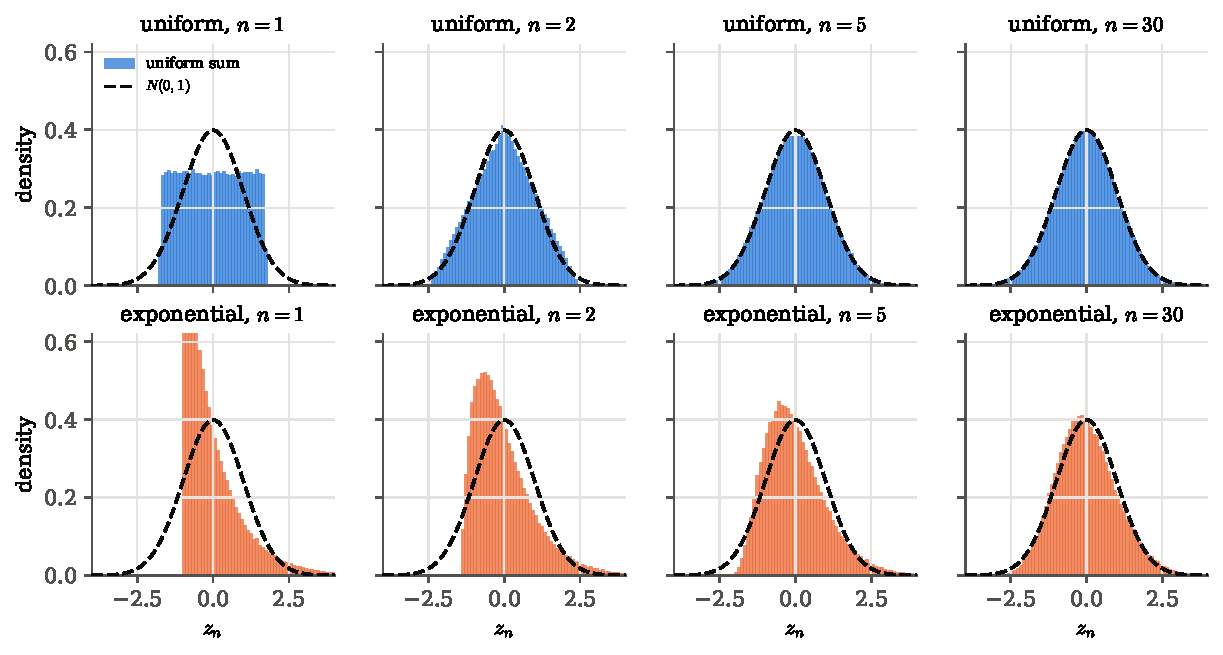
\includegraphics[width=\linewidth]{figures/ch02/clt_histograms.pdf}
\caption{Histograms of the standardised sum $z_n$ of $n$ uniforms (top) and $n$ exponentials (bottom), $\tbCLTnsamp$ experiments each, with the standard normal density (dashed). The uniform sum is already bell-shaped at $n=2$ to $5$. The exponential sum keeps a visible skew, a steep left side and a long right tail, even at $n=30$.}
\label{2b:fig:clt-hist}
\end{figure}

\begin{figure}[htbp]
\centering
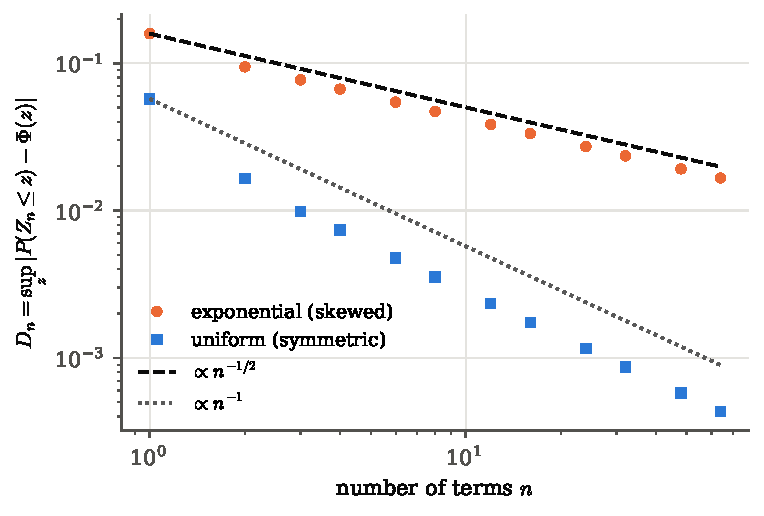
\includegraphics[width=0.66\linewidth]{figures/ch02/clt_rate.pdf}
\caption{The worst-case gap between the distribution of $z_n$ and $\Phi$, as a function of the number of terms. For the skewed exponential parent it falls as $n^{-1/2}$ (dashed), for the symmetric uniform parent as $n^{-1}$ (dotted). At $n=30$ the symmetric case is more than twenty times closer to Gaussian.}
\label{2b:fig:clt-rate}
\end{figure}

\paragraph{What this bought us.}
``Large $n$'' is not a number; it depends on the skewness of what is being added. The error of the Gaussian approximation is about $0.07\,\gamma_1/\sqrt n$ in cumulative probability. Symmetric ingredients converge like $1/n$, lopsided ones like $1/\sqrt n$.

\subsection{Where the theorem fails: Breit--Wigner resonances}
\label{2b:sec:cauchy}

\paragraph{Measuring the Z mass with a running average.}
The invariant mass of $e^+e^-$ pairs from Z decays follows, to a first approximation, the (non-relativistic) \newterm{Breit--Wigner} or \newterm{Cauchy} line shape
\begin{equation}
  p(m\given M,\Gamma)=\frac1\pi\frac{\Gamma/2}{(m-M)^2+\Gamma^2/4},
  \label{2b:eq:bw}
\end{equation}
with $M=91.1876$\,GeV the mass and $\Gamma=2.4952$\,GeV the full width at half maximum \srcref{Cowan}{(2.41)}. (We ignore detector resolution and radiation to keep the point clean.) A student averages the masses of the first $N$ events and expects the average to settle down like $1/\sqrt N$.

The student's expectation fails, because the Breit--Wigner has no mean. It is a proper density: with $u=2(m-M)/\Gamma$, $\int\frac{\dd u}{\pi(1+u^2)}=\frac1\pi[\arctan u]_{-\infty}^{\infty}=1$ \mainref{p.~30}. But the two halves of the mean, $\int_M^\infty m\,p(m)\dd m$ and $\int_{-\infty}^M m\,p(m)\dd m$, diverge separately, because the integrand falls only like $1/m$. Their difference is therefore undefined \srcref{Cowan}{p.~36--37}; CasellaBerger's (3.3.20) states it as $\E|X|=\infty$. The variance is infinite too, so the CLT does not apply.

Instead, the mean of Cauchy variables is as wide as one of them. If $X_1,\dots,X_n$ are iid Cauchy with centre $M$ and half-width $\gamma=\Gamma/2$, then $\bar X_n$ has \emph{exactly the same} Cauchy distribution, for every $n$ \srcref{CasellaBerger}{p.~177}. Averaging does not help at all.

The proof is two lines once we have the characteristic function. For the standard Cauchy $p(x)=1/[\pi(1+x^2)]$ and $k>0$, close the contour in the upper half plane, where $e^{ikx}$ decays, around the pole at $x=i$:
\begin{align}
  \phi(k)
  &\eqby{1} \frac1\pi\oint\frac{e^{ikx}}{(x-i)(x+i)}\dd x
  \eqby{2} \frac1\pi\,2\pi i\,\frac{e^{ik\cdot i}}{2i}
  = e^{-k} ,
  \label{2b:eq:cf-cauchy}
\end{align}
\begin{explain}
  \item Factor $1+x^2$. The semicircle at infinity contributes nothing for $k>0$.
  \item Residue theorem: $2\pi i$ times the residue at $x=i$, which is $e^{ik\,i}/(i+i)$.
\end{explain}
and by symmetry $\phi(k)=e^{-|k|}$ for all $k$ \srcref{Cowan}{Table~10.1}. For centre $M$ and scale $\gamma$, $\phi(k)=e^{iMk-\gamma|k|}$. Then
\begin{align}
  \phi_{\bar X_n}(k)
  &\eqby{1}\Bigl[\phi\Bigl(\frac kn\Bigr)\Bigr]^n
  \eqby{2}\Bigl[e^{iMk/n-\gamma|k|/n}\Bigr]^n
  = e^{iMk-\gamma|k|} ,
  \label{2b:eq:cauchy-mean}
\end{align}
\begin{explain}
  \item Product and scaling rules with $a=1/n$.
  \item The Cauchy characteristic function at frequency $k/n$.
\end{explain}
which is the characteristic function of a single event. \emph{Where did the CLT proof break?} At the expansion. The kink of $e^{-|k|}$ at $k=0$ is the Fourier-space signature of the missing variance: $\phi$ has no second derivative there, so the expansion \eqref{2b:eq:cf-taylor} does not exist \srcref{Cowan}{p.~145}. The width is controlled by $|k|$ rather than $k^2$. So in the exponent it scales as $n\times\frac1n=1$, instead of the $n\times\frac1{n^2}$ that would have made it shrink.

\paragraph{One event can move the average anywhere.}
With a Gaussian, an event $10\sigma$ away is essentially impossible. With a Breit--Wigner, the probability of landing further than $t$ from the peak falls only like $1/t$. Among $N$ events, the most extreme one is typically at distance $\sim N\gamma$ from the peak, so its contribution to the average, $\sim N\gamma/N=\gamma$, never becomes small. The average is always at the mercy of the latest outlier. The \emph{median} does not care how far out an outlier is, only on which side it lies.

The simulation shows both behaviours. The script draws $10^5$ Breit--Wigner masses in three independent streams. After $10^5$ events one running mean sits at $\tbBWfinalMean$\,GeV, $\tbBWfinalOff$\,GeV from the true mass, and all three keep jumping (\cref{2b:fig:cauchy}a). The running median of the same events is $\tbBWfinalMedian$\,GeV. Its standard error, $\pi\gamma/(2\sqrt N)=\tbBWmedSE$\,GeV, does fall like $1/\sqrt N$: the median of any continuous density has asymptotic variance $1/[4Np(M)^2]$, and $p(M)=1/(\pi\gamma)$ here. Panel (b) repeats the average of $\tbBWnavg$ events twenty thousand times: its interquartile range is $\tbBWiqrMean$\,GeV, equal to that of a \emph{single} event, $2\gamma=\Gamma=\tbBWiqrTheory$\,GeV.

\pyfile[firstline=41,lastline=50,firstnumber=41]{code/ch02/22_cauchy_landau.py}{Running mean and running median of Breit--Wigner masses}

Line 42 generates Breit--Wigner masses as $M+\gamma\,C$, where $\gamma=\Gamma/2$ is the half-width and $C$ is a standard Cauchy variable. Numpy draws $C$ with
\pyname{rng.standard_cauchy}. (A standard Cauchy variable is the same thing as the ratio of two independent standard normals.) Line 43 computes all running means at once with a cumulative sum. Line 49 evaluates the running median on a logarithmic grid of $N$ values.

\begin{figure}[htbp]
\centering
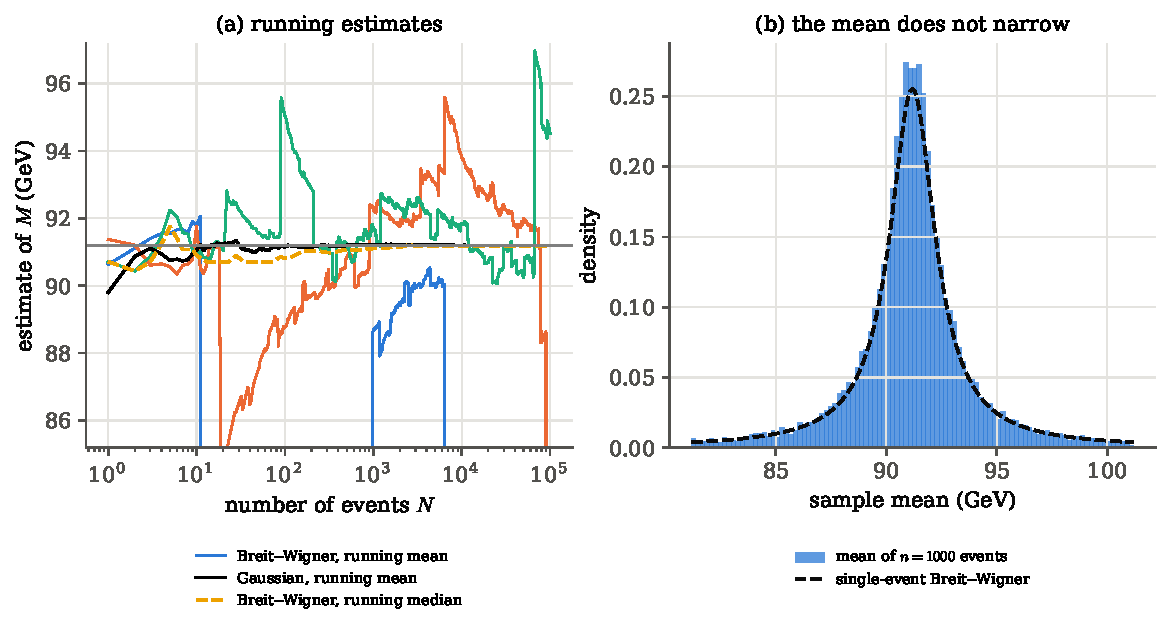
\includegraphics[width=\linewidth]{figures/ch02/cauchy_running.pdf}
\caption{(a) Running estimates of the Z mass from Breit--Wigner events. The three coloured running means jump by GeV every time an extreme event arrives and never settle. The running mean of Gaussian events of the same half-width (black) and the running median of the Breit--Wigner events (dashed) both converge to the true mass (grey line). (b) The distribution of the average of $1000$ events (histogram) is the single-event Breit--Wigner (dashed): no narrowing at all.}
\label{2b:fig:cauchy}
\end{figure}

\begin{pitfall}[The width convention]
Cowan's $\Gamma$ in \eqref{2b:eq:bw} is the \emph{full} width at half maximum, the convention of particle physics, where $\Gamma=\hbar/\tau$ is the decay rate. Many statistics texts write the Cauchy scale $\gamma$ as the \emph{half} width, and \pyname{scipy.stats.cauchy(loc, scale)} expects $\gamma=\Gamma/2$ \srcref{Cowan}{p.~37, footnote}.
\end{pitfall}

Strictly, real resonances do have a mean. The mass cannot be negative or exceed the collision energy, and the relativistic line shape with phase space and parton luminosities cuts the tails \srcref{Cowan}{p.~38--39}. But the cut sits so far out that the practical lesson stands: sample means of resonance masses converge painfully slowly and are dominated by a few events. Fit the line shape, or use the median or a truncated mean.

\subsection{Where the theorem is slow: Landau energy loss}
\label{2b:sec:landau}

A charged particle crossing a thin layer loses energy $\Delta$ in many soft collisions and, occasionally, one hard collision that knocks out a fast $\delta$-electron. The distribution of $\Delta$, derived by Landau, is \srcref{Cowan}{(2.42)--(2.46)}
\begin{equation}
  f(\Delta)=\frac1\xi\,\phi_L(\lambda),\qquad
  \lambda=\frac1\xi\Bigl[\Delta-\xi\Bigl(\ln\frac{\xi}{\epsilon'}+1-\gamma_E\Bigr)\Bigr],\qquad
  \phi_L(\lambda)=\frac1\pi\int_0^\infty e^{-u\ln u-\lambda u}\sin\pi u\,\dd u ,
  \label{2b:eq:landau}
\end{equation}
where $\xi$ grows with the layer thickness and falls like $1/\beta^2$ ($\beta$ is the particle's speed in units of $c$), $\epsilon'$ depends on the ionisation energy of the material and on $\beta\gamma$, and $\gamma_E=0.5772$ is Euler's constant. The high tail falls like $1/\lambda^2$, following the Rutherford cross-section for hard knock-ons. So, as for the Breit--Wigner, the mean and variance do not exist. The useful number is the most probable loss, $\Delta_{\mathrm{mp}}=\xi[\ln(\xi/\epsilon')+0.198]$ \srcref{Cowan}{(2.48)}. It depends on the velocity, and it is the basis of particle identification by $\dd E/\dd x$.

Adding layers does not make the Landau tail Gaussian. Cowan's example \srcref{Cowan}{p.~148}: the ionisation in $1$\,m of argon is the sum over $25$ layers of $4$\,cm, and one might hope the sum is Gaussian. The script adds $\tbLanNlayers$ standard Landau variables and compares the result with a Gaussian of the same median and interquartile range (\cref{2b:fig:landau}). The core matches. The tail does not: a fraction $\tbLanTailFrac$ of the sums lie more than five matched standard deviations above the median, against $\tbLanTailGauss$ for a Gaussian. Rare hard collisions dominate the sum however many layers we add. (Mathematically the Landau distribution is \emph{stable}: like the Cauchy, the suitably shifted and rescaled sum of Landau variables is again Landau.) Practical $\dd E/\dd x$ estimators therefore use a truncated mean, discarding the largest $30$--$40\%$ of the samples.

\begin{figure}[htbp]
\centering
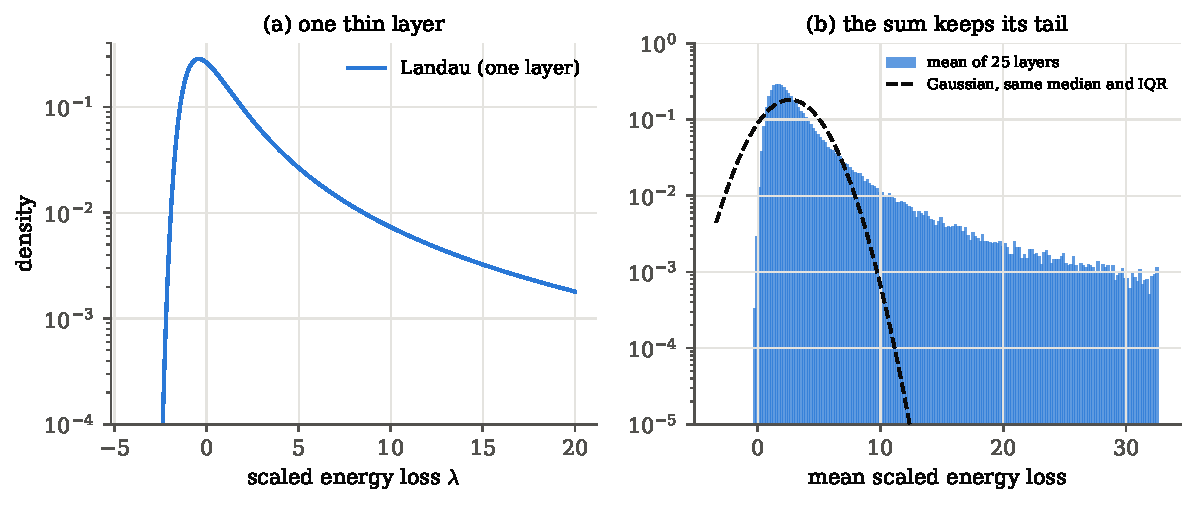
\includegraphics[width=\linewidth]{figures/ch02/landau_sum.pdf}
\caption{(a) The Landau density for one thin layer, on a logarithmic scale: a sharp peak and a long power-law tail to high energy loss. (b) The mean over $25$ layers (histogram) against a Gaussian with the same median and interquartile range (dashed). The Gaussian describes the core and misses the tail by many orders of magnitude.}
\label{2b:fig:landau}
\end{figure}

\begin{taxonomy}[Does the CLT apply to my sum?]
\begin{tabular}{@{}p{0.43\linewidth}p{0.51\linewidth}@{}}
\toprule
situation & what the sum does \\
\midrule
independent, identical, finite variance & Gaussian; error $\approx0.07\gamma_1/\sqrt n$ in probability \\
independent, different variances, none dominant & Gaussian (Lindeberg), variance $\sum\sigma_j^2$ \\
one term dominates the variance & looks like that term \\
infinite variance (Breit--Wigner, Landau, power-law tails) & no Gaussian limit; a \emph{stable} law with the same heavy tail \\
correlated terms & Gaussian only if correlations die off, with an \emph{effective} $n$ smaller than $n$ \\
a \emph{product} of positive factors & log-normal: apply the CLT to the logarithm (\cref{2b:sec:zoo}) \\
the \emph{maximum}, not the sum & not Gaussian at all: extreme-value laws (Gumbel, Fr\'echet, Weibull) \\
\bottomrule
\end{tabular}
\end{taxonomy}

\paragraph{How research uses this.}
The sums of uniforms and exponentials \emph{verify} a theorem whose answer we know. The same machinery becomes the research instrument when the ingredients are the actual detector effects. Cowan's warning \srcref{Cowan}{p.~148} is that a quoted ``$1\sigma$'' interval covers $68.3\%$ only if the errors are Gaussian in their tails. The only way to learn the tails of a real resolution function (multiple Coulomb scattering has a Gaussian core and a single-scattering Rutherford tail) is a detailed Monte Carlo of the individual contributions. In cosmology the band-power $\Chat$ is a sum of $2\ell+1$ squared Gaussian modes. At high $\ell$ the CLT makes it Gaussian; at low $\ell$ it is visibly skewed, and the likelihood of the CMB power spectrum has to be built with that skewness in it \cite{HamimecheLewis2008} (\cref{ch:07,ch:08}). Gravitational-wave detector noise is Gaussian in bulk, but ``glitches'' play the role of the Landau tail and must be vetoed or modelled.

\section{The Gaussian, third way: the least committal assignment}
\label{2b:sec:maxent}

A calibration note says: ``the timing resolution of the chamber is $2$\,ns rms.'' Nothing more. No histogram, no list of contributions, no statement about tails. Yet the next step of every analysis is to write down a probability density for the timing residual, because a likelihood needs one. Which density should we write? The first two derivations of the Gaussian do not help here. De Moivre--Laplace needs a binomial, and the central limit theorem needs a sum of many independent pieces. Here we know neither. We know one number.

The third reason the Gaussian is everywhere is of a different kind. It is not about how the noise was produced. It is about what we \emph{know}. The principle of maximum entropy picks out the one distribution that agrees with the facts we have and assumes nothing else. With it we can write a density when all we have is a mean, or a variance, or a covariance matrix. It shows why least squares, which is a Gaussian likelihood, is the natural fit when all we know is the size of the error bars. And it is the same variational principle that produces the Boltzmann distribution in statistical mechanics, so it rests on physics we already trust.

The question, stated in words: \emph{among all distributions that satisfy a set of known averages, which one should we use, and what does it look like when the known average is a variance?}

\subsection{A die with a loaded average}
\label{2b:sec:maxent-die}

Start with Sivia's example, because it is discrete and we can see every number \srcref{Sivia}{p.~113--114}. A six-sided die has been rolled very many times. We are told only that the average number of dots was $4.5$. What probabilities $p_1,\dots,p_6$ should we assign to the six faces?

The information is a single linear constraint,
\begin{equation}
  \sum_{i=1}^{6} i\,p_i = 4.5 ,\qquad \sum_{i=1}^{6}p_i=1 .
  \label{2b:eq:die-constraint}
\end{equation}
The fair die, $p_i=1/6$, has average $3.5$, so it is ruled out. But infinitely many assignments remain. Here are three of them:
\begin{itemize}
  \item $p=(0,0,0,\tfrac12,\tfrac12,0)$: only faces 4 and 5 ever appear. The average is $4.5$.
  \item $p=(0,0,\tfrac12,0,0,\tfrac12)$: only faces 3 and 6 appear. The average is $\tfrac32+3=4.5$.
  \item Something smooth that rises steadily from face 1 to face 6.
\end{itemize}
The first two are absurd. They claim that faces 1, 2, 3 and 6 (or 1, 2, 4 and 5) \emph{never} appear, and nothing we were told supports that. They contain information we do not have. The third kind feels right. It leans towards the high faces just enough to move the average from $3.5$ to $4.5$, and otherwise treats the faces evenhandedly. To turn ``feels right'' into a rule, we need a number that measures how much an assignment commits to beyond the constraints. Then we pick the assignment for which that number is smallest.

\subsection{Why the measure is the entropy: counting the ways}
\label{2b:sec:monkeys}

Sivia's ``monkey argument'' \srcref{Sivia}{p.~116--118} derives that number by counting, exactly as Boltzmann counted microstates. Imagine $M$ boxes, one per possible outcome, and a team of monkeys throwing $N$ pennies into them completely at random, each penny into each box with probability $1/M$. After the throw, box $i$ holds $n_i$ pennies, with $\sum_i n_i=N$, and we read off the candidate assignment
\begin{equation}
  p_i=\frac{n_i}{N}.
  \label{2b:eq:monkey-p}
\end{equation}
If the candidate violates the constraint we throw it away. If it satisfies it we keep it. Repeat many times. The assignment the monkeys produce most often is the one we should use. \emph{Why?} The monkeys have no preferences. So whatever structure the favoured assignment has beyond the constraint, it has only because overwhelmingly many throws produce it.

How often do the monkeys produce a given set of occupation numbers $\{n_i\}$? There are $M^N$ equally likely sequences of throws (each of $N$ pennies picks one of $M$ boxes). The number of sequences that put $n_1$ pennies in box 1, $n_2$ in box 2, and so on, is the multinomial coefficient of \cref{2a:sec:multinomial}. So the frequency is
\begin{equation}
  F(\{p_i\})=\frac{1}{M^N}\,\frac{N!}{n_1!\,n_2!\cdots n_M!} .
  \label{2b:eq:monkey-F}
\end{equation}
Now let $N$ be very large, so that every $n_i$ is large too, and use Stirling's formula in its crudest form $\ln n!\approx n\ln n-n$ (the leading terms of \eqref{2b:eq:stirling}):
\begin{align}
  \ln F
  &\eqby{1} -N\ln M+\ln N!-\sum_{i=1}^M\ln n_i! \nonumber\\
  &\eqby{2} -N\ln M+\bigl(N\ln N-N\bigr)-\sum_{i=1}^M\bigl(n_i\ln n_i-n_i\bigr) \nonumber\\
  &\eqby{3} -N\ln M+N\ln N-\sum_{i=1}^M n_i\ln n_i \nonumber\\
  &\eqby{4} -N\ln M-\sum_{i=1}^M n_i\ln\frac{n_i}{N} \nonumber\\
  &\eqby{5} -N\ln M-N\sum_{i=1}^M p_i\ln p_i .
  \label{2b:eq:monkey-lnF}
\end{align}
\begin{explain}
  \item Logarithm of \eqref{2b:eq:monkey-F}: a quotient becomes a difference and a product becomes a sum.
  \item Stirling, $\ln n!\approx n\ln n-n$, for $N!$ and for each $n_i!$. The neglected terms grow only like $\ln n$, which is negligible next to $n$.
  \item The $-N$ and the $+\sum_i n_i=+N$ cancel.
  \item Write $N\ln N=\sum_i n_i\ln N$ (again because $\sum_in_i=N$) and combine the two logarithms.
  \item Substitute $n_i=Np_i$ from \eqref{2b:eq:monkey-p}.
\end{explain}
The first term, $-N\ln M$, is the same for every candidate. So the monkeys produce the assignment $\{p_i\}$ with a frequency proportional to $e^{NS}$, where
\begin{equation}
  S=-\sum_{i=1}^M p_i\ln p_i .
  \label{2b:eq:entropy-discrete}
\end{equation}
Because $N$ is huge, $e^{NS}$ is extremely sharply peaked. Two candidates whose values of $S$ differ by only $0.01$ are produced with frequencies in the ratio $e^{0.01N}$, which for $N=10^4$ pennies is $e^{100}$. Among all candidates that pass the constraint, essentially only the one with the largest $S$ ever comes out. This is the same mathematics that makes the equilibrium macrostate of a gas overwhelmingly the most probable: Boltzmann's $S=k_B\ln W$ with $W$ the number of microstates is \eqref{2b:eq:monkey-lnF} with $k_B=1$.

\paragraph{Unequal boxes.} When the possible outcomes are not equally likely to begin with, the entropy acquires a reference distribution. So far all boxes were the same size. Suppose instead that the proposition ``the face shows 3, 4, 5 or 6'' is one box and ``the face shows 1'' and ``shows 2'' are two more. Then a fair monkey should hit the big box four times as often \srcref{Sivia}{p.~118--119}. If box $i$ is hit with probability $m_i$ (with $\sum_i m_i=1$), the frequency \eqref{2b:eq:monkey-F} becomes the full multinomial probability $\frac{N!}{\prod_i n_i!}\prod_i m_i^{n_i}$, and the same Stirling steps give
\begin{equation}
  \frac1N\ln F=-\sum_{i=1}^M p_i\ln\frac{p_i}{m_i} .
  \label{2b:eq:entropy-measure}
\end{equation}
The only new term is $+\sum_i n_i\ln m_i=N\sum_ip_i\ln m_i$, and it joins the logarithm. When all $m_i=1/M$ we recover \eqref{2b:eq:entropy-discrete} up to the constant $\ln M$.

\begin{workdef}[entropy of a distribution, and the MaxEnt principle]
The \newterm{entropy} of a discrete assignment $\{p_i\}$ relative to a \newterm{measure} $\{m_i\}$ \unpack{the probabilities we would assign if we knew nothing at all, often equal} is
\[
  S=-\sum_i p_i\ln\frac{p_i}{m_i}.
\]
For a continuous variable with density $p(x)$ and measure $m(x)$ it is \srcref{Sivia}{(5.29)}
\begin{equation}
  S[p]=-\int p(x)\ln\frac{p(x)}{m(x)}\,\dd x .
  \label{2b:eq:entropy-cont}
\end{equation}
The \newterm{principle of maximum entropy} (MaxEnt): given \newterm{testable information} \unpack{constraints of the form $\E f_k(X)=F_k$, which any proposed distribution either obeys or violates}, assign the distribution that maximises $S$ subject to those constraints and to normalisation.
\emph{Operational recipe:} write $p\propto m\,e^{-\sum_k\lambda_kf_k}$ and solve the constraint equations for the multipliers $\lambda_k$.
\end{workdef}

The continuous formula needs the measure $m(x)$ because a density has units. If $x$ is a time in ns and we switch to seconds, $p(x)$ is multiplied by $10^9$, and $-\int p\ln p\,\dd x$ shifts by $-\ln 10^9$. The ratio $p/m$ has no units, since $p$ and $m$ transform the same way under a change of variable. So \eqref{2b:eq:entropy-cont} is the same number in any coordinates \srcref{Sivia}{p.~119}. What is $m$? Maximising $S$ with only the normalisation constraint gives $p=m$ (Sivia's (5.30), and the case $K=0$ of the recipe below). So $m$ is the distribution of complete ignorance. For a location variable on the real line it is uniform, and then we may drop it. From now on we do so unless we say otherwise.

\subsection{The recipe: Lagrange multipliers give exponentials}
\label{2b:sec:maxent-recipe}

Maximising the entropy under known averages always gives an exponential. To see why, maximise $S$ with $K$ testable constraints $\sum_i p_i f_k(x_i)=F_k$, $k=1,\dots,K$. We handle the constraints with Lagrange multipliers \unpack{one extra unknown per constraint, chosen at the end so the constraint holds}: find the stationary point of
\begin{equation*}
  Q=-\sum_i p_i\ln\frac{p_i}{m_i}+\lambda_0\Bigl(1-\sum_i p_i\Bigr)+\sum_{k=1}^K\lambda_k\Bigl(F_k-\sum_i p_i f_k(x_i)\Bigr).
\end{equation*}
Differentiate with respect to one particular $p_j$. Only the terms containing $p_j$ contribute:
\begin{align}
  \frac{\partial Q}{\partial p_j}
  &\eqby{1} -\ln\frac{p_j}{m_j}-1-\lambda_0-\sum_{k=1}^K\lambda_kf_k(x_j) \eqby{2} 0 \nonumber\\
  \Longrightarrow\quad p_j
  &\eqby{3} m_j\,e^{-(1+\lambda_0)}\,\exp\Bigl[-\sum_{k=1}^K\lambda_kf_k(x_j)\Bigr]
   \eqby{4} \frac{m_j}{Z}\exp\Bigl[-\sum_{k=1}^K\lambda_kf_k(x_j)\Bigr].
  \label{2b:eq:maxent-solution}
\end{align}
\begin{explain}
  \item $\frac{\dd}{\dd p}(-p\ln(p/m))=-\ln(p/m)-1$, and each constraint is linear in $p_j$ with coefficient $-1$ or $-f_k(x_j)$.
  \item A maximum of $Q$ is a stationary point.
  \item Exponentiate and multiply by $m_j$.
  \item Normalisation fixes $e^{1+\lambda_0}=Z\equiv\sum_j m_j\exp[-\sum_k\lambda_kf_k(x_j)]$, the \newterm{partition function}.
\end{explain}
Is it a maximum and not a minimum? Yes, and the only one. The second derivatives are $\partial^2Q/\partial p_j\partial p_l=-\delta_{jl}/p_j<0$, so $Q$ is strictly concave, and a concave function on the convex set of allowed $\{p_i\}$ has exactly one stationary point, its global maximum. There is no risk of picking a saddle.

Every physicist has seen \eqref{2b:eq:maxent-solution} before. With one constraint, the mean energy $\sum_ip_iE_i=U$, it reads $p_j=e^{-\beta E_j}/Z$, the Boltzmann distribution, with the Lagrange multiplier $\beta$ playing the role of $1/k_BT$. Temperature \emph{is} the Lagrange multiplier that enforces a given mean energy. Jaynes's reading of statistical mechanics, which Sivia summarises \srcref{Sivia}{p.~118}, is exactly this: the canonical ensemble is the least committal assignment compatible with a known average energy.

\paragraph{Example: the die.} For the die, $m_i=1/6$ and there is one constraint, $f(i)=i$, $F=4.5$. Writing $\lambda\equiv-\lambda_1$ for convenience, \eqref{2b:eq:maxent-solution} says
\begin{equation}
  p_i=\frac{e^{\lambda i}}{Z(\lambda)},\qquad Z(\lambda)=\sum_{j=1}^6 e^{\lambda j},\qquad
  \sum_{i=1}^6 i\,p_i=\frac{\dd\ln Z}{\dd\lambda}=4.5 .
  \label{2b:eq:die-maxent}
\end{equation}
This equation for $\lambda$ has exactly one solution. The mean $\dd\ln Z/\dd\lambda$ increases with $\lambda$, because its derivative $\dd^2\ln Z/\dd\lambda^2=\sum i^2p_i-(\sum ip_i)^2$ is a variance and so positive. At $\lambda=0$ the mean is $3.5$, and as $\lambda\to\infty$ it tends to $6$. So it passes $4.5$ exactly once, and a root finder gives $\lambda=\tbMElam$. The probabilities are
\[
  (p_1,\dots,p_6)=(\tbMEpOne,\ \tbMEpTwo,\ \tbMEpThree,\ \tbMEpFour,\ \tbMEpFive,\ \tbMEpSix),
\]
a geometric progression with ratio $e^\lambda\approx1.45$: every step up in dots multiplies the probability by the same factor (\cref{2b:fig:maxent-die}a, which reproduces Sivia's Fig.~5.2). The entropy is $S=\tbMESmax$, below the fair-die value $\ln6=\tbMESuniformDie$: the constraint costs entropy, as it must.

\paragraph{Checking by brute force.} No random die with the same average beats the MaxEnt die. The script draws $4\times10^6$ random assignments uniformly over all possible dice (a Dirichlet$(1,\dots,1)$ distribution, which we meet in \cref{2b:sec:zoo}). It keeps the $\tbMEnKeep$ whose mean lies within $0.005$ of $4.5$, and \cref{2b:fig:maxent-die}b histograms their entropies. The largest entropy among them is $\tbMESrandMax$ (for a die of mean $\tbMESrandMaxMean$), against $\tbMESmax$ for the MaxEnt die. The two are very close, and a random die can even come out a hair ahead. That is not a defeat: the window lets in means slightly below $4.5$, closer to the fair $3.5$, and a smaller tilt costs less entropy. Comparing like with like, each candidate against the MaxEnt die of \emph{its own} mean, every one falls short, by at least $\tbMEminDeficit$.

\pyfile[firstline=38,lastline=51,firstnumber=38]{code/ch02/23_maxent.py}{The MaxEnt die, and random dice with the same mean}

Lines 38--40 compute the mean $\sum_i i\,p_i$ of the exponential family \eqref{2b:eq:die-maxent} for a given $\lambda$. Line 43 solves ``mean $=4.5$'' for $\lambda$ with Brent's bracketing root finder; the monotonicity argument above is what guarantees that the bracket $[-5,5]$ contains exactly one root. Lines 49--51 draw random dice, keep those with the right mean, and compute their entropies, using the convention $0\ln0=0$.

\begin{figure}[htbp]
\centering
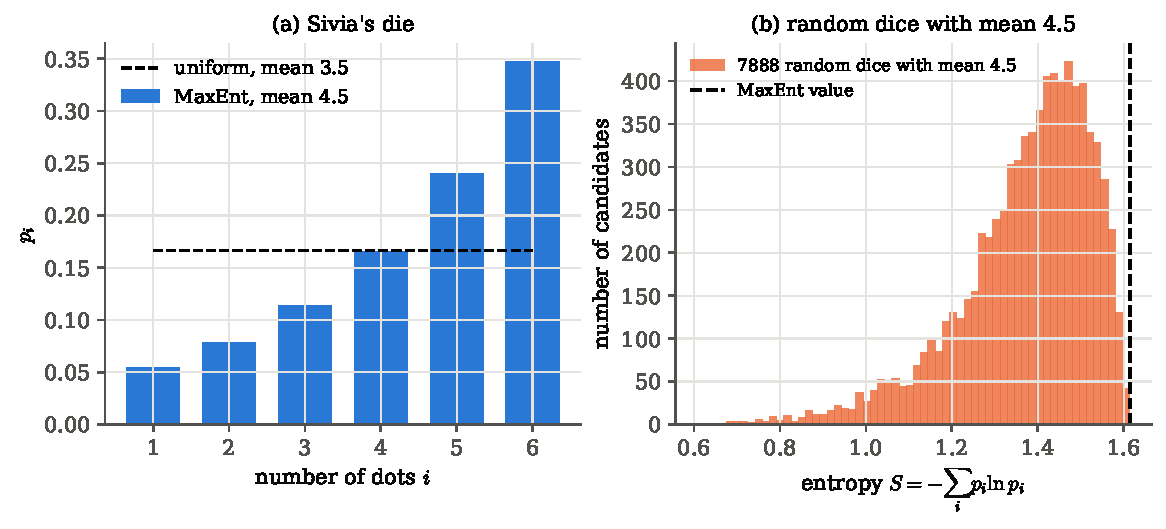
\includegraphics[width=\linewidth]{figures/ch02/maxent_die.pdf}
\caption{(a) The maximum-entropy die for a known average of $4.5$ (bars) against the fair die (dashed). The probabilities grow by a constant factor from face to face. (b) Entropies of several thousand randomly drawn dice whose average is also $4.5$. They pile up to the left of the MaxEnt value (dashed line), and compared with the MaxEnt die of its own average every one falls short: every other assignment assumes something extra.}
\label{2b:fig:maxent-die}
\end{figure}

\paragraph{Example: the kangaroo problem.} Is entropy really special, or would any function that rewards spreading out do? Sivia's kangaroo problem answers this \srcref{Sivia}{p.~114--116}. We are told that one third of all kangaroos have blue eyes and one third are left-handed. What fraction are both? Call the four probabilities $p_1$ (blue, left), $p_2$ (blue, right), $p_3$ (not blue, left), $p_4$ (not blue, right). The two facts and normalisation leave one free number, $x=p_1$ (\cref{2b:fig:kangaroo}a):
\[
  p_1=x,\quad p_2=\tfrac13-x,\quad p_3=\tfrac13-x,\quad p_4=\tfrac13+x,\qquad 0\le x\le\tfrac13 .
\]
Common sense says $x=1/9$: with no information about a link between eye colour and handedness, we should not invent one, and independence gives $\frac13\times\frac13$. Maximise the entropy:
\begin{align}
  \frac{\dd S}{\dd x}
  &\eqby{1} \frac{\dd}{\dd x}\Bigl[-x\ln x-2\bigl(\tfrac13-x\bigr)\ln\bigl(\tfrac13-x\bigr)-\bigl(\tfrac13+x\bigr)\ln\bigl(\tfrac13+x\bigr)\Bigr] \nonumber\\
  &\eqby{2} -\ln x-1+2\ln\bigl(\tfrac13-x\bigr)+2-\ln\bigl(\tfrac13+x\bigr)-1 \nonumber\\
  &\eqby{3} \ln\frac{(\tfrac13-x)^2}{x(\tfrac13+x)} .
  \label{2b:eq:kangaroo}
\end{align}
\begin{explain}
  \item Entropy \eqref{2b:eq:entropy-discrete} of the four-cell table.
  \item $\frac{\dd}{\dd x}(-u\ln u)=-(\ln u+1)\,\frac{\dd u}{\dd x}$, with $\frac{\dd u}{\dd x}=+1,-1,-1,+1$ for the four cells.
  \item The constants cancel ($-1+2-1=0$) and the logarithms combine.
\end{explain}
Setting this to zero gives $(\frac13-x)^2=x(\frac13+x)$, that is $\frac19-\frac23x+x^2=\frac13x+x^2$, so $x=\frac19$. Entropy reproduces independence exactly.

Other plausible-looking criteria do not. Maximising $-\sum p_i^2$ gives $\frac{\dd}{\dd x}\bigl[x^2+2(\frac13-x)^2+(\frac13+x)^2\bigr]=8x-\frac23=0$, so $x=\frac1{12}$: a negative correlation nobody asked for. The script maximises all four of Sivia's candidates numerically and finds $x=\tbKangEnt$ (entropy), $\tbKangSq$ ($-\sum p_i^2$), $\tbKangLog$ ($\sum\ln p_i$) and $\tbKangSqrt$ ($\sum\sqrt{p_i}$), reproducing his Table~5.1. Only functions monotonically related to $S$ give $1/9$ (Sivia quotes Skilling for the proof), and that is the strongest argument that entropy is the right measure of ``assuming nothing extra''.

\begin{figure}[htbp]
\centering
\begin{tikzpicture}
  \begin{scope}
    \draw[thick] (0,0) rectangle (3.2,3.2);
    \draw[thick] (1.6,0) -- (1.6,3.2);
    \draw[thick] (0,1.6) -- (3.2,1.6);
    \node[lbl] at (0.8,2.4) {$x$};
    \node[lbl] at (2.4,2.4) {$\tfrac13-x$};
    \node[lbl] at (0.8,0.8) {$\tfrac13-x$};
    \node[lbl] at (2.4,0.8) {$\tfrac13+x$};
    \node[lbl,anchor=south] at (0.8,3.25) {left};
    \node[lbl,anchor=south] at (2.4,3.25) {right};
    \node[lbl,anchor=east] at (-0.05,2.4) {blue};
    \node[lbl,anchor=east] at (-0.05,0.8) {not blue};
    \node[lbl,font=\small\bfseries] at (1.6,-1.75) {(a)};
  \end{scope}
  \begin{scope}[xshift=5.0cm,yshift=-0.2cm]
  \begin{axis}[width=7.0cm,height=4.6cm,xmin=0,xmax=0.3333,ymin=0.6,ymax=1.34,
      xlabel={$x=p_1$},ylabel={entropy $S$},
      xtick={0,0.1111,0.2222,0.3333},xticklabels={$0$,$\frac19$,$\frac29$,$\frac13$},
      tick label style={font=\scriptsize},label style={font=\small},
      legend style={font=\scriptsize,at={(0.6,0.03)},anchor=south,draw=none,fill=none}]
    \addplot[formblue,thick,domain=0.0005:0.3328,samples=200]
      {-x*ln(x)-2*(1/3-x)*ln(1/3-x)-(1/3+x)*ln(1/3+x)};
    \addlegendentry{$S(x)$}
    \addplot[only marks,mark=*,mark size=1.6pt,fibreorange,samples at={0.0833,0.1218,0.1301}]
      {-x*ln(x)-2*(1/3-x)*ln(1/3-x)-(1/3+x)*ln(1/3+x)};
    \addlegendentry{other criteria}
    \addplot[only marks,mark=square*,mark size=2pt,black,samples at={0.1111}]
      {-x*ln(x)-2*(1/3-x)*ln(1/3-x)-(1/3+x)*ln(1/3+x)};
    \addlegendentry{maximum, $x=\frac19$}
    \draw[faint,dashed] (axis cs:0.1111,0.6) -- (axis cs:0.1111,1.273);
  \end{axis}
  \node[lbl,font=\small\bfseries] at (2.6,-1.55) {(b)};
  \end{scope}
\end{tikzpicture}
\caption{The kangaroo problem. (a) The two known marginals, one third blue-eyed and one third left-handed, leave a single free number $x$ in the $2\times2$ table. (b) The entropy of the table as a function of $x$. It peaks at $x=1/9$, the independent answer. The orange dots mark the maximisers of Sivia's three alternative criteria, which all build in a correlation that the information does not contain.}
\label{2b:fig:kangaroo}
\end{figure}

\subsection{Continuous MaxEnt: a variance gives a Gaussian}
\label{2b:sec:maxent-gauss}

Back to the timing residual of the calibration note, where all we were given was an rms of $2$\,ns. The testable information is that the residual $x$ has mean $\mu$ and variance $\sigma^2$, and $x$ can be any real number. The question: which density has the largest entropy under these two constraints? The continuous version of the recipe replaces sums by integrals and the partial derivative by a functional derivative \unpack{the change of $Q$ when $p$ is changed by a small bump $\delta p$ at one point $x$, divided by the area of the bump}. We need
\[
  Q[p]=-\int p\ln p\,\dd x+\lambda_0\Bigl(1-\int p\,\dd x\Bigr)+\lambda_1\Bigl(\sigma^2-\int(x-\mu)^2p\,\dd x\Bigr)
\]
to be stationary \srcref{Sivia}{p.~121--122}. Then
\begin{align}
  \frac{\delta Q}{\delta p(x)}
  &\eqby{1} -\ln p(x)-1-\lambda_0-\lambda_1(x-\mu)^2 \eqby{2} 0
  \quad\Longrightarrow\quad p(x)=e^{-1-\lambda_0}\,e^{-\lambda_1(x-\mu)^2} , \nonumber\\
  1&\eqby{3} e^{-1-\lambda_0}\int_{-\infty}^{\infty}e^{-\lambda_1(x-\mu)^2}\dd x
   \eqby{4} e^{-1-\lambda_0}\sqrt{\frac{\pi}{\lambda_1}} , \nonumber\\
  \sigma^2&\eqby{5} \sqrt{\frac{\lambda_1}{\pi}}\int_{-\infty}^{\infty}(x-\mu)^2e^{-\lambda_1(x-\mu)^2}\dd x
   \eqby{6} \frac{1}{2\lambda_1}
  \quad\Longrightarrow\quad
  p(x)=\frac{1}{\sqrt{2\pi\sigma^2}}\,e^{-(x-\mu)^2/2\sigma^2}.
  \label{2b:eq:maxent-gauss}
\end{align}
\begin{explain}
  \item The same differentiation as in \eqref{2b:eq:maxent-solution}, applied pointwise: changing $p$ near $x$ changes each integral by its integrand at $x$ times the size of the change.
  \item Stationarity; then solve for $p$. For the integral to exist we need $\lambda_1>0$.
  \item The normalisation constraint.
  \item The Gaussian integral \eqref{2b:eq:gauss-integral}, rescaled: substitute $z=\sqrt{2\lambda_1}(x-\mu)$.
  \item The variance constraint, with the constant from line (4), $e^{-1-\lambda_0}=\sqrt{\lambda_1/\pi}$.
  \item The normalised density $\sqrt{\lambda_1/\pi}\,e^{-\lambda_1(x-\mu)^2}$ is a Gaussian of variance $1/(2\lambda_1)$, by \eqref{2b:eq:gauss-moments}. Solving $\sigma^2=1/(2\lambda_1)$ gives $\lambda_1=1/(2\sigma^2)$.
\end{explain}
So the maximum-entropy density with a given mean and variance is the Gaussian $\Normal(\mu,\sigma^2)$ of \eqref{2b:eq:gauss}. Nothing was assumed about how the residual was produced.

\paragraph{A second proof, and a proof that it is the maximum.} The Lagrange argument finds a stationary point. A short inequality shows directly that no other density with the same variance does better. We use one elementary fact, $\ln t\le t-1$ for $t>0$ (the tangent line at $t=1$ lies above the concave logarithm). Let $p$ be any density with mean $\mu$ and variance $\sigma^2$, and let $g$ be the Gaussian with the same two numbers. Then
\begin{align}
  S[p]-S[g]
  &\eqby{1} -\int p\ln p\,\dd x+\int g\ln g\,\dd x \nonumber\\
  &\eqby{2} -\int p\ln p\,\dd x+\int p\ln g\,\dd x \nonumber\\
  &\eqby{3} \int p\ln\frac{g}{p}\,\dd x \nonumber\\
  &\relby{4}{\le} \int p\Bigl(\frac gp-1\Bigr)\dd x \eqby{5} \int g\,\dd x-\int p\,\dd x = 0 .
  \label{2b:eq:gibbs}
\end{align}
\begin{explain}
  \item Definition \eqref{2b:eq:entropy-cont} with uniform measure.
  \item $\ln g(x)=-\frac12\ln(2\pi\sigma^2)-(x-\mu)^2/2\sigma^2$ is a constant plus a multiple of $(x-\mu)^2$. Its average is therefore fixed by the normalisation and the variance alone, and $p$ and $g$ share both.
  \item Combine the two integrals.
  \item $\ln t\le t-1$ with $t=g/p$, at every $x$ where $p>0$.
  \item Both densities integrate to one.
\end{explain}
Equality in step (4) needs $g/p=1$ everywhere, so the Gaussian is the \emph{unique} maximiser. The quantity $\int p\ln(p/g)\,\dd x\ge0$ we just met is the \newterm{Kullback--Leibler divergence} of $p$ from $g$. It will return in \cref{ch:03} (maximum likelihood minimises it) and in \cref{ch:05}. The value itself is
\[
  S[g]=-\int g\ln g\,\dd x\eqby{1}\tfrac12\ln(2\pi\sigma^2)+\frac{\E(x-\mu)^2}{2\sigma^2}=\tfrac12\ln\bigl(2\pi e\sigma^2\bigr),
\]
where (1) inserts $\ln g$ from step (2) above.

\begin{keyidea}[The third origin of the Gaussian]
Of all densities on the real line with a given mean $\mu$ and variance $\sigma^2$, the Gaussian $\Normal(\mu,\sigma^2)$ has the largest entropy, $\tfrac12\ln(2\pi e\sigma^2)$. Assigning it claims nothing about the data except the mean and the variance. Assigning anything else claims more.
\end{keyidea}

\paragraph{Example: five densities with unit variance.} The script evaluates the entropy of five familiar densities, each scaled to variance one: uniform $\tbEntUniform$, Laplace $\tbEntLaplace$, triangular $\tbEntTriang$, logistic $\tbEntLogistic$, Gaussian $\tbEntGauss=\frac12\ln(2\pi e)$. The Gaussian wins, but the others are close. The logistic is only $0.014$ behind: two densities with nearly the same core can have nearly the same entropy. \Cref{2b:fig:unitvar} shows three of the five, and why they lose. The uniform ``wastes'' its variance by having no tails at all. The Laplace concentrates probability in a cusp and pays for its variance with long exponential tails. The Gaussian spreads its probability in the most even way the variance allows.

\begin{figure}[htbp]
\centering
\begin{tikzpicture}
\begin{axis}[width=10cm,height=5cm,xmin=-4,xmax=4,ymin=0,ymax=0.75,
    xlabel={$x$ (units of $\sigma$)},ylabel={density},
    tick label style={font=\scriptsize},label style={font=\small},
    legend style={font=\scriptsize,at={(0.99,0.97)},anchor=north east,draw=none,fill=none}]
  \addplot[formblue,very thick,domain=-4:4,samples=201] {exp(-x^2/2)/sqrt(2*pi)};
  \addlegendentry{Gaussian, $S=\tbEntGauss$}
  \addplot[fibreorange,thick,domain=-4:4,samples=401] {exp(-sqrt(2)*abs(x))/sqrt(2)};
  \addlegendentry{Laplace, $S=\tbEntLaplace$}
  \addplot[tangentgreen,thick] coordinates {(-4,0) (-1.7321,0) (-1.7321,0.2887) (1.7321,0.2887) (1.7321,0) (4,0)};
  \addlegendentry{uniform, $S=\tbEntUniform$}
\end{axis}
\end{tikzpicture}
\caption{Three densities with the same mean ($0$) and variance ($1$). The uniform box stops dead at $\pm\sqrt3$; the Laplace density has a sharp peak and fat exponential tails. Among all densities with this variance the Gaussian has the largest entropy, and the numbers in the legend show by how much it beats these two.}
\label{2b:fig:unitvar}
\end{figure}

\subsection{The family tree: other constraints, other distributions}
\label{2b:sec:maxent-family}

Each common distribution is the MaxEnt answer to some piece of partial knowledge. The recipe \eqref{2b:eq:maxent-solution} works like a machine: feed in the constraint functions $f_k$ and the range of $x$, and out comes $p\propto m\,e^{-\sum\lambda_kf_k}$. Sivia runs it for the common cases \srcref{Sivia}{p.~120--125}:
\begin{itemize}
  \item \emph{Nothing but the range $[a,b]$.} Then $p=m$, the uniform density $1/(b-a)$ (Bernoulli's principle of insufficient reason).
  \item \emph{A mean $\mu$, with $x\ge0$.} One constraint $f=x$, so $p\propto e^{-\lambda_1x}$. Normalisation on $[0,\infty)$ gives $\lambda_1e^{-\lambda_1x}$ and the mean gives $\lambda_1=1/\mu$: the exponential $p(x)=\mu^{-1}e^{-x/\mu}$ \srcref{Sivia}{(5.33)}, the waiting-time law of \eqref{2a:eq:expo}. The same computation on the line with a mean alone fails: $e^{-\lambda_1x}$ cannot be normalised on $(-\infty,\infty)$, which is the recipe's way of saying that a mean alone does not specify a spread.
  \item \emph{A variance on the whole line.} The Gaussian, \eqref{2b:eq:maxent-gauss}.
  \item \emph{A mean absolute deviation $\E|x-\mu|=\epsilon$.} $f=|x-\mu|$ gives the Laplace (double-exponential) density $\frac{1}{2\epsilon}e^{-|x-\mu|/\epsilon}$ \srcref{Sivia}{(5.39)--(5.40)}. Its log-likelihood is $-\sum|x_k-\mu_k|/\epsilon_k$: the $\ell_1$ ``least absolute deviations'' fit, which is more robust to outliers than least squares.
  \item \emph{Many variables with known individual variances.} With $N$ data $x_k$, predictions $\mu_k$ and known $\E(x_k-\mu_k)^2=\sigma_k^2$, the multidimensional version gives the product of Gaussians \srcref{Sivia}{(5.36)--(5.38)}
  \begin{equation}
    p(\{x_k\})=\prod_{k=1}^N\frac{1}{\sqrt{2\pi}\sigma_k}\exp\Bigl[-\frac{(x_k-\mu_k)^2}{2\sigma_k^2}\Bigr],
    \label{2b:eq:maxent-lsq}
  \end{equation}
  which is exactly the likelihood behind least squares, $-2\ln p=\chi^2+\text{const}$. From the MaxEnt point of view least squares does not assume that the noise \emph{is} Gaussian. It is the honest likelihood when all we know is the size of each error bar. If we also know the covariances $\E(x_j-\mu_j)(x_k-\mu_k)$, the same recipe returns the correlated multivariate Gaussian of the next section.
  \item \emph{A mean count $\E N=\mu$ of events in an interval.} Here the measure matters. Cut the interval into $M$ tiny cells, each of which can hold an event or not. The number of cell patterns giving $N$ events among $M$ indistinguishable cells is $M^N/N!$ for $M\gg N$, so $m(N)\propto M^N/N!$ \srcref{Sivia}{(5.43)}. Then
  \[
    p(N)\propto\frac{M^N}{N!}e^{-\lambda N}=\frac{(Me^{-\lambda})^N}{N!}
    \quad\Longrightarrow\quad
    p(N)=e^{-\mu}\frac{\mu^N}{N!},
  \]
  where normalisation, $\sum_N(Me^{-\lambda})^N/N!=e^{Me^{-\lambda}}$, and the mean condition identify $Me^{-\lambda}=\mu$. The unknown $M$ drops out, and we recover the Poisson distribution of \cref{2a:sec:poisson-limit} from knowledge of the mean alone.
  \item \emph{The mean kinetic energy of a gas molecule.} The constraint $\E\frac12m|\bm v|^2=\frac32k_BT$ with uniform measure on velocity space gives a Gaussian for each velocity component with variance $k_BT/m$. The speed distribution that follows is the Maxwell--Boltzmann law of \cref{2b:sec:zoo}.
\end{itemize}

\begin{pitfall}[MaxEnt is a statement about knowledge, not about the noise]
The MaxEnt Gaussian is the best assignment \emph{given only} a variance. If the real residuals have a Landau tail (\cref{2b:sec:landau}) or a Breit--Wigner shape, the Gaussian will misjudge the tails badly, and the cure is not to argue about entropy but to put the extra knowledge in as a constraint (a known tail fraction, a known fourth moment) or to model the mechanism. And when the variance is infinite, as for a Breit--Wigner, there is no variance constraint to impose in the first place.
\end{pitfall}

\paragraph{How the three origins fit together.} The three reasons for the Gaussian agree, and that is not a coincidence. De Moivre--Laplace and the central limit theorem are statements about \emph{mechanisms}: many small independent contributions added together. MaxEnt is a statement about \emph{information}: we know a variance and nothing else. The link is that adding independent pieces and rescaling to fixed variance can only increase the entropy (convolution smooths). So the central limit theorem is the dynamics that drives a sum towards the maximum-entropy state, like a gas relaxing to equilibrium. When a physicist writes ``Gaussian errors'' she is usually relying on all of them at once: the CLT for why the errors should be close to Gaussian, and MaxEnt for why, knowing only the error bar, nothing else would be more honest.

The same principle supplies the forward model $P(\data\given\params)$, the probability of the data $\data$ given the parameters $\params$, whenever only the covariance of the noise is known. The prior assignments of \cref{ch:05} use it too. And the MaxEnt die's exponential form is the first example of the exponential families that make maximum likelihood and conjugate priors tractable (\cref{ch:03,ch:05}).
\section{Many correlated Gaussians: the multivariate normal}
\label{2b:sec:mvn}

Most measurements come as several numbers that move together, and one object describes them all: the multivariate Gaussian. A straight-line track fit returns two numbers, an intercept and a slope, and they are never independent: tilt the line a little and the intercept has to move to keep the line going through the hits. A fit of a CMB power spectrum returns $\Omega_m h^2$ and $n_s$, and they, too, move together. A CMB temperature map is a list of $10^6$ pixel values, each Gaussian, and neighbouring pixels are strongly correlated. A stretch of gravitational-wave strain is a list of $10^5$ samples whose correlations are set by the detector's noise spectrum. The Fisher matrix of \cref{ch:10} approximates every posterior by a multivariate Gaussian, and a Gaussian random field (\cref{ch:07}) is a multivariate Gaussian with very many components.

Four things about it are used constantly. How to \emph{sample} it, which follows from building it out of independent standard normals. The shape of its contours, the ellipses of every parameter-estimation plot. What fraction of the probability each ellipse contains. And two operations: \emph{marginalising} (averaging out a nuisance variable) and \emph{conditioning} (fixing one variable at a known value).

The questions, in words: \emph{what is the joint density of several correlated Gaussian quantities, how do we draw from it, and what are the distributions of a subset of them, either ignoring the rest or with the rest held fixed?}

\subsection{Building it: a linear map of independent standard normals}
\label{2b:sec:mvn-build}

Start from what we know. Let $Z_1,\dots,Z_k$ be independent $\Normal(0,1)$ variables and collect them into a column vector $\bm Z$. Independence means the joint density is the product of the one-dimensional densities \mainref{p.~40}:
\begin{equation}
  p_{\bm Z}(\bm z)=\prod_{j=1}^k\frac{e^{-z_j^2/2}}{\sqrt{2\pi}}=\frac{1}{(2\pi)^{k/2}}\exp\Bigl(-\tfrac12\bm z\T\bm z\Bigr).
  \label{2b:eq:mvn-std}
\end{equation}
Its contours, $\bm z\T\bm z=\text{const}$, are spheres, and its components are uncorrelated. Correlations appear when we mix the components linearly. Take a fixed invertible $k\times k$ matrix $\mathbf A$ and a fixed vector $\bm\mu$ and define
\begin{equation}
  \bm X=\bm\mu+\mathbf A\bm Z .
  \label{2b:eq:mvn-map}
\end{equation}
Its mean is $\E\bm X=\bm\mu+\mathbf A\,\E\bm Z=\bm\mu$. Its covariance matrix \unpack{the $k\times k$ table of all $\Cov(X_i,X_j)$, with the variances on the diagonal} is
\begin{align}
  \Cmat\equiv\E\bigl[(\bm X-\bm\mu)(\bm X-\bm\mu)\T\bigr]
  &\eqby{1} \E\bigl[\mathbf A\bm Z\bm Z\T\mathbf A\T\bigr]
  \eqby{2} \mathbf A\,\E\bigl[\bm Z\bm Z\T\bigr]\mathbf A\T
  \eqby{3} \mathbf A\mathbf A\T .
  \label{2b:eq:mvn-cov}
\end{align}
\begin{explain}
  \item $\bm X-\bm\mu=\mathbf A\bm Z$, and $(\mathbf A\bm Z)\T=\bm Z\T\mathbf A\T$.
  \item $\mathbf A$ is not random, and expectation is linear, so it can be taken outside on both sides.
  \item $\E(Z_iZ_j)=\delta_{ij}$: unit variances and, by independence, zero covariances. So $\E\bm Z\bm Z\T=\Id$.
\end{explain}
We know the mean and covariance of $\bm X$; now we want its density. Change variables. The map $\bm z\mapsto\bm x=\bm\mu+\mathbf A\bm z$ is linear with inverse $\bm z=\mathbf A^{-1}(\bm x-\bm\mu)$. A small box of volume $\dd^k z$ is mapped to a parallelepiped of volume $|\det\mathbf A|\,\dd^kz$, so probability conservation, $p_{\bm X}\,\dd^kx=p_{\bm Z}\,\dd^kz$, gives
\begin{align}
  p_{\bm X}(\bm x)
  &\eqby{1} p_{\bm Z}\bigl(\mathbf A^{-1}(\bm x-\bm\mu)\bigr)\,\frac{1}{|\det\mathbf A|} \nonumber\\
  &\eqby{2} \frac{1}{(2\pi)^{k/2}|\det\mathbf A|}\exp\Bigl[-\tfrac12(\bm x-\bm\mu)\T(\mathbf A^{-1})\T\mathbf A^{-1}(\bm x-\bm\mu)\Bigr] \nonumber\\
  &\eqby{3} \frac{1}{(2\pi)^{k/2}(\det\Cmat)^{1/2}}\exp\Bigl[-\tfrac12(\bm x-\bm\mu)\T\Cmat^{-1}(\bm x-\bm\mu)\Bigr].
  \label{2b:eq:mvn}
\end{align}
\begin{explain}
  \item The multidimensional change-of-variables rule: the Jacobian of the inverse map is $\det\mathbf A^{-1}=1/\det\mathbf A$.
  \item Insert \eqref{2b:eq:mvn-std} with $\bm z=\mathbf A^{-1}(\bm x-\bm\mu)$, so $\bm z\T\bm z=(\bm x-\bm\mu)\T(\mathbf A^{-1})\T\mathbf A^{-1}(\bm x-\bm\mu)$.
  \item $(\mathbf A^{-1})\T\mathbf A^{-1}=(\mathbf A\mathbf A\T)^{-1}=\Cmat^{-1}$, and $\det\Cmat=\det\mathbf A\,\det\mathbf A\T=(\det\mathbf A)^2$.
\end{explain}
The matrix $\mathbf A$ has disappeared: only $\Cmat=\mathbf A\mathbf A\T$ is left. So the distribution is fixed by the mean and the covariance alone, and any two matrices with the same $\mathbf A\mathbf A\T$ give the same distribution. That is the density quoted by all our sources \mainref{(2.10)}, \srcref{Cowan}{(2.28)}.

\begin{workdef}[multivariate normal distribution]
A random vector $\bm X\in\R^k$ is \newterm{multivariate normal}, $\bm X\sim\Normal(\bm\mu,\Cmat)$, if its density is \eqref{2b:eq:mvn}, where $\bm\mu$ is its mean vector and $\Cmat$ its covariance matrix, which must be symmetric and \newterm{positive definite} \unpack{$\bm a\T\Cmat\bm a>0$ for every nonzero vector $\bm a$. This says that every linear combination $\bm a\T\bm X$ has a nonzero variance}. It has $k$ means plus $k(k+1)/2$ independent entries of $\Cmat$ as parameters \srcref{Cowan}{p.~33}.
\emph{Operational recipe (sampling):} factor $\Cmat=\mathbf L\mathbf L\T$ (Cholesky, $\mathbf L$ lower triangular, or the symmetric square root $\Cmat^{1/2}$ of \mainref{Thm~2.43}), draw $k$ independent standard normals $\bm z$, and return $\bm\mu+\mathbf L\bm z$. \emph{Inverse (whitening):} $\mathbf L^{-1}(\bm X-\bm\mu)\sim\Normal(0,\Id)$.
\end{workdef}

Why must $\Cmat$ be positive definite? Because $\bm a\T\Cmat\bm a=\Var(\bm a\T\bm X)$, and a variance cannot be negative. If it is zero for some $\bm a\neq0$, then $\bm a\T\bm X$ is a constant: one component is an exact linear function of the others, the distribution lives on a lower-dimensional plane, $\det\Cmat=0$, and \eqref{2b:eq:mvn} does not exist. (A fitted $\Cmat$ that is singular or nearly singular almost always means a parameter that the data cannot distinguish from a combination of the others.)

\paragraph{Example: two dimensions, written out.} For $k=2$ write $\Cmat=\begin{pmatrix}\sigma_x^2&\rho\sigma_x\sigma_y\\ \rho\sigma_x\sigma_y&\sigma_y^2\end{pmatrix}$, where $\rho=\Cov(x,y)/(\sigma_x\sigma_y)$ is the \newterm{correlation coefficient}, $-1<\rho<1$. The inverse of a $2\times2$ matrix is its adjugate over its determinant, so with $u=(x-\mu_x)/\sigma_x$ and $v=(y-\mu_y)/\sigma_y$,
\begin{align}
  (\bm x-\bm\mu)\T\Cmat^{-1}(\bm x-\bm\mu)
  &\eqby{1} \frac{1}{\sigma_x^2\sigma_y^2(1-\rho^2)}
    \begin{pmatrix}x-\mu_x& y-\mu_y\end{pmatrix}
    \begin{pmatrix}\sigma_y^2&-\rho\sigma_x\sigma_y\\-\rho\sigma_x\sigma_y&\sigma_x^2\end{pmatrix}
    \begin{pmatrix}x-\mu_x\\ y-\mu_y\end{pmatrix} \nonumber\\
  &\eqby{2} \frac{u^2-2\rho uv+v^2}{1-\rho^2} ,
  \label{2b:eq:bvn-quad}
\end{align}
\begin{explain}
  \item $\det\Cmat=\sigma_x^2\sigma_y^2-\rho^2\sigma_x^2\sigma_y^2=\sigma_x^2\sigma_y^2(1-\rho^2)$, and the adjugate swaps the diagonal entries and flips the sign of the off-diagonal ones.
  \item Multiply out: the three terms are $\sigma_y^2(x-\mu_x)^2$, $-2\rho\sigma_x\sigma_y(x-\mu_x)(y-\mu_y)$ and $\sigma_x^2(y-\mu_y)^2$; dividing each by $\sigma_x^2\sigma_y^2$ turns them into $u^2$, $-2\rho uv$, $v^2$.
\end{explain}
and $(\det\Cmat)^{1/2}=\sigma_x\sigma_y\sqrt{1-\rho^2}$. This gives the bivariate normal density of \srcref{Cowan}{(2.30)} and \srcref{CasellaBerger}{Def.~4.5.10},
\begin{equation}
  p(x,y)=\frac{1}{2\pi\sigma_x\sigma_y\sqrt{1-\rho^2}}\exp\Bigl[-\frac{u^2-2\rho uv+v^2}{2(1-\rho^2)}\Bigr].
  \label{2b:eq:bvn}
\end{equation}
Our running example, used by the script and in the rest of this section, has $\sigma_x=1$, $\sigma_y=2$, $\rho=0.8$ (and means $\mu_x=1$, $\mu_y=2$), so $\Cmat=\begin{pmatrix}1&1.6\\1.6&4\end{pmatrix}$ and $\det\Cmat=4-2.56=1.44$. Its Cholesky factor is $\mathbf L=\begin{pmatrix}1&0\\1.6&1.2\end{pmatrix}$; check: $\mathbf L\mathbf L\T=\begin{pmatrix}1&1.6\\1.6&1.6^2+1.2^2\end{pmatrix}=\Cmat$. So a sample is $x=\mu_x+z_1$, $y=\mu_y+1.6z_1+1.2z_2$: the $y$ component copies $80\%$ of the $x$ fluctuation, in units of its own width, and adds fresh noise of its own. That sentence is what a correlation of $0.8$ \emph{means} mechanically.

\subsection{The shape: ellipses and how much they contain}
\label{2b:sec:mvn-ellipse}

The contours of the multivariate Gaussian are ellipsoids, and rotating to their axes removes the correlations. To see this, note that the density \eqref{2b:eq:mvn} depends on $\bm x$ only through the quadratic form
\[
  Q(\bm x)=(\bm x-\bm\mu)\T\Cmat^{-1}(\bm x-\bm\mu),
\]
so its contours are the surfaces $Q=c$. To find their shape, diagonalise $\Cmat$. A real symmetric matrix has an orthonormal basis of eigenvectors: $\Cmat=\mathbf R\,\boldsymbol\Lambda\,\mathbf R\T$ with $\mathbf R$ a rotation whose columns are the eigenvectors and $\boldsymbol\Lambda=\diag(\lambda_1,\dots,\lambda_k)$, all $\lambda_i>0$ by positive definiteness. In rotated coordinates $\bm y=\mathbf R\T(\bm x-\bm\mu)$,
\begin{equation}
  Q\eqby{1}\bm y\T\boldsymbol\Lambda^{-1}\bm y\eqby{2}\sum_{i=1}^k\frac{y_i^2}{\lambda_i}=c ,
  \label{2b:eq:mvn-ellipse}
\end{equation}
\begin{explain}
  \item $\Cmat^{-1}=\mathbf R\boldsymbol\Lambda^{-1}\mathbf R\T$ because $\mathbf R^{-1}=\mathbf R\T$.
  \item $\boldsymbol\Lambda^{-1}$ is diagonal.
\end{explain}
an ellipsoid with principal axes along the eigenvectors and semi-axes $\sqrt{c\lambda_i}$. In the $y$ coordinates the components are independent, $y_i\sim\Normal(0,\lambda_i)$: rotating to the eigenbasis \emph{removes} the correlations. This is the same step as finding the normal modes of coupled oscillators.

For the running example ($\sigma_x=1$, $\sigma_y=2$, $\rho=0.8$), the eigenvalues solve $\lambda^2-(\tr\Cmat)\lambda+\det\Cmat=\lambda^2-5\lambda+1.44=0$, so $\lambda=\frac12\bigl(5\pm\sqrt{25-5.76}\bigr)$, that is $\lambda_1=\tbMVNlamOne$ and $\lambda_2=\tbMVNlamTwo$. The major axis, from $(1-\lambda_1)v_1+1.6v_2=0$, has slope $v_2/v_1=(\lambda_1-1)/1.6=2.31$, an angle of $\tbMVNangle^\circ$ from the $x$ axis.

\paragraph{How much probability is inside an ellipse?} The question reduces to one about the length of a standard normal vector. Whiten: $\bm Z=\mathbf L^{-1}(\bm X-\bm\mu)$, with $\mathbf L$ the Cholesky factor of $\Cmat$, is a vector of independent standard normals, and $Q=\bm Z\T\bm Z$ (the calculation in step (3) of \eqref{2b:eq:mvn}, read backwards). So the probability inside $Q\le c$ is the probability that a $k$-dimensional standard normal vector has squared length at most $c$. In \cref{2b:sec:chi2} we will show that this squared length has the $\chi^2_k$ distribution \mainref{Thm~2.44(4)}. For $k=2$ we can do it at once in polar coordinates, exactly as in \eqref{2b:eq:gauss-integral}:
\begin{align}
  \Prob(Q\le c)
  &\eqby{1}\int_0^{2\pi}\!\!\int_0^{\sqrt c}\frac{e^{-r^2/2}}{2\pi}\,r\,\dd r\,\dd\phi
   \eqby{2}\Bigl[-e^{-r^2/2}\Bigr]_0^{\sqrt c}
   = 1-e^{-c/2} .
  \label{2b:eq:ellipse-content}
\end{align}
\begin{explain}
  \item $Q=z_1^2+z_2^2=r^2$, and the density \eqref{2b:eq:mvn-std} with $k=2$ is $e^{-r^2/2}/2\pi$.
  \item The angular integral gives $2\pi$, and $r\,e^{-r^2/2}$ has antiderivative $-e^{-r^2/2}$.
\end{explain}
Setting $1-e^{-c/2}$ equal to the one-dimensional $1\sigma$ and $2\sigma$ probabilities, $0.6827$ and $0.9545$, gives $c=-2\ln(1-0.6827)=\tbMVNlevOne$ and $c=\tbMVNlevTwo$. These are the familiar $\Delta\chi^2=2.30$ and $6.18$ contours of two-parameter plots. So the ellipse $Q=1$, which is often drawn as the ``$1\sigma$ ellipse'', is too small: it contains only $1-e^{-1/2}=39.3\%$. In $k$ dimensions the required $c$ grows further. A random vector in many dimensions is almost never near its centre, because the $\chi^2_k$ distribution of its squared length has mean $k$.

\paragraph{Reading the ellipse: marginal box, conditional chord.} One ellipse carries two different error bars for $y$, and they must not be confused. \Cref{2b:fig:ellipse-geometry} is drawn with the true numbers of the running example. \emph{The box.} The ellipse $Q=1$ is tangent to the box $|x-\mu_x|\le\sigma_x$, $|y-\mu_y|\le\sigma_y$. (Check the top point: with $x-\mu_x=z_1$, $y-\mu_y=1.6z_1+1.2z_2$ and $z_1=\cos t$, $z_2=\sin t$, $y$ is largest when $\tan t=1.2/1.6$, giving $y-\mu_y=1.6\times0.8+1.2\times0.6=2=\sigma_y$.) So the projection of the $Q=1$ ellipse on each axis is the marginal $\pm1\sigma$ range. \emph{The chord.} The vertical chord through the centre is shorter: at $x=\mu_x$ the ellipse has $y-\mu_y=\pm1.2=\pm\sigma_y\sqrt{1-\rho^2}$, which, as \cref{2b:sec:mvn-conditional} shows, is the $1\sigma$ range of $y$ when $x$ is \emph{known}. \emph{The tilt.} The points where the ellipse has vertical tangents, $(\mu_x\pm1,\mu_y\pm1.6)$, lie on the line $y-\mu_y=\rho(\sigma_y/\sigma_x)(x-\mu_x)$, the conditional mean. This line is \emph{not} the major axis: its angle is $\arctan1.6=58^\circ$, not $\tbMVNangle^\circ$.

\begin{figure}[htbp]
\centering
\begin{tikzpicture}[scale=1.25]
  \draw[faint,->] (-2.2,0) -- (2.4,0) node[anchor=west,lbl] {$x-\mu_x$};
  \draw[faint,->] (0,-2.6) -- (0,2.7) node[anchor=south,lbl] {$y-\mu_y$};
  \draw[fibreorange,thick,dashed] (-1,-2) rectangle (1,2);
  \draw[formblue,very thick,samples=120,domain=0:360,smooth]
    plot ({cos(\x)},{1.6*cos(\x)+1.2*sin(\x)});
  \draw[bdryred,thick] (-1.45,-2.32) -- (1.45,2.32);
  \fill[bdryred] (1,1.6) circle (1.4pt) (-1,-1.6) circle (1.4pt);
  \draw[vec] (0,0) -- ({2.166*cos(66.6)},{2.166*sin(66.6)});
  \draw[vec] (0,0) -- ({0.554*cos(156.6)},{0.554*sin(156.6)});
  \draw[black,line width=1.6pt] (0,-1.2) -- (0,1.2);
  \node[lbl,anchor=west,fibreorange] at (1.05,-1.75) {marginal box: $\pm\sigma_x$, $\pm\sigma_y$};
  \node[lbl,anchor=west,bdryred] at (1.5,2.35) {$\E(y\given x)$, slope $\rho\sigma_y/\sigma_x$};
  \node[lbl,anchor=east] at (-1.1,-0.6) {heavy chord: $\pm\sigma_y\sqrt{1-\rho^2}$};
  \node[lbl,anchor=east,tangentgreen] at (-1.1,0.6) {green: principal axes};
  \node[lbl,anchor=west,formblue] at (1.1,-0.7) {$Q=1$};
\end{tikzpicture}
\caption{The $Q=1$ contour of the example ($\sigma_x=1$, $\sigma_y=2$, $\rho=0.8$), drawn exactly. It just touches the dashed box of the marginal $\pm1\sigma$ ranges. The heavy vertical chord at $x=\mu_x$ is the much shorter $\pm1\sigma$ range of $y$ once $x$ is fixed. The red line of conditional means passes through the two points of vertical tangency (dots), and it is tilted less steeply than the long principal axis (green).}
\label{2b:fig:ellipse-geometry}
\end{figure}

\subsection{Linear combinations and marginals}
\label{2b:sec:mvn-marginal}

Every linear function of a Gaussian vector is again Gaussian, and marginals are a special case. The quickest proof uses the characteristic function, the $k$-dimensional version of \eqref{2b:eq:cf}, $\phi_{\bm X}(\bm t)=\E e^{i\bm t\T\bm X}$. With $\bm X=\bm\mu+\mathbf A\bm Z$,
\begin{align}
  \phi_{\bm X}(\bm t)
  &\eqby{1} e^{i\bm t\T\bm\mu}\,\E\exp\bigl(i(\mathbf A\T\bm t)\T\bm Z\bigr)
   \eqby{2} e^{i\bm t\T\bm\mu}\prod_{j=1}^k e^{-(\mathbf A\T\bm t)_j^2/2}
   \eqby{3} \exp\Bigl(i\bm t\T\bm\mu-\tfrac12\bm t\T\Cmat\,\bm t\Bigr).
  \label{2b:eq:mvn-cf}
\end{align}
\begin{explain}
  \item $\bm t\T\mathbf A\bm Z=(\mathbf A\T\bm t)\T\bm Z$, and the constant phase comes out of the expectation.
  \item The $Z_j$ are independent, so the expectation factorises, and each factor is the one-dimensional Gaussian characteristic function $e^{-s^2/2}$ \eqref{2b:eq:cf-gauss} at $s=(\mathbf A\T\bm t)_j$.
  \item $\sum_j(\mathbf A\T\bm t)_j^2=\bm t\T\mathbf A\mathbf A\T\bm t=\bm t\T\Cmat\bm t$.
\end{explain}
Now let $\mathbf B$ be any $m\times k$ matrix and $\bm Y=\mathbf B\bm X$. Its characteristic function is $\E e^{i\bm s\T\mathbf B\bm X}=\phi_{\bm X}(\mathbf B\T\bm s)=\exp(i\bm s\T\mathbf B\bm\mu-\frac12\bm s\T\mathbf B\Cmat\mathbf B\T\bm s)$, which is again of the form \eqref{2b:eq:mvn-cf}. Since the characteristic function determines the distribution,
\begin{equation}
  \bm X\sim\Normal(\bm\mu,\Cmat)\quad\Longrightarrow\quad \mathbf B\bm X\sim\Normal\bigl(\mathbf B\bm\mu,\;\mathbf B\Cmat\mathbf B\T\bigr).
  \label{2b:eq:mvn-linear}
\end{equation}
Two special cases are the ones everybody uses \mainref{Thm~2.44}, \srcref{CasellaBerger}{p.~144}.
\begin{itemize}
  \item A single linear combination, $\mathbf B=\bm a\T$: $\bm a\T\bm X\sim\Normal(\bm a\T\bm\mu,\bm a\T\Cmat\bm a)$. For two variables, $ax+by\sim\Normal(a\mu_x+b\mu_y,\ a^2\sigma_x^2+b^2\sigma_y^2+2ab\rho\sigma_x\sigma_y)$. This is the exact form of the error-propagation formula for linear functions.
  \item The marginal of a subset. Split $\bm X=(\bm X_a,\bm X_b)$ and $\bm\mu$, $\Cmat$ into the matching blocks $\bm\mu_a$, $\Cmat_{aa}$, $\Cmat_{ab}$, and so on. Choosing $\mathbf B=(\Id\;\;0)$ picks out $\bm X_a$, and $\mathbf B\Cmat\mathbf B\T=\Cmat_{aa}$. So $\bm X_a\sim\Normal(\bm\mu_a,\Cmat_{aa})$.
\end{itemize}
The second statement is marginalising in exactly the sense of \cref{ch:01}. In words: to average out the nuisance variables $\bm X_b$ of a Gaussian, \emph{delete their rows and columns} from $\bm\mu$ and $\Cmat$. No integral needs to be done. In the running example the marginal of $y$ is $\Normal(\mu_y,4)$ whatever the value of $\rho$; the script finds a sample standard deviation of $\tbMVNmargSd$ for $y$.

\subsection{Conditionals: fixing one variable}
\label{2b:sec:mvn-conditional}

Suppose we learn the value of $\bm X_a$ exactly. What is the distribution of $\bm X_b$ now? Split $\bm X_b$ into the part that $\bm X_a$ can predict and a residual that it cannot. Define the residual
\[
  \bm W=\bm X_b-\Cmat_{ba}\Cmat_{aa}^{-1}\bm X_a .
\]
$\bm W$ and $\bm X_a$ are uncorrelated:
\begin{align}
  \Cov(\bm W,\bm X_a)
  &\eqby{1} \Cov(\bm X_b,\bm X_a)-\Cmat_{ba}\Cmat_{aa}^{-1}\Cov(\bm X_a,\bm X_a)
   \eqby{2} \Cmat_{ba}-\Cmat_{ba}\Cmat_{aa}^{-1}\Cmat_{aa}=0 .
  \label{2b:eq:mvn-uncorr}
\end{align}
\begin{explain}
  \item Covariance is linear in each argument, and $\Cmat_{ba}\Cmat_{aa}^{-1}$ is a constant matrix.
  \item The blocks of $\Cmat$ are exactly these covariances.
\end{explain}
For Gaussians, uncorrelated means independent. The vector $(\bm W,\bm X_a)$ is a linear function of $\bm X$, so by \eqref{2b:eq:mvn-linear} it is jointly Gaussian, and its covariance matrix is block diagonal by \eqref{2b:eq:mvn-uncorr}. A block-diagonal $\Cmat$ has a block-diagonal inverse and a determinant equal to the product of the blocks' determinants, so the density \eqref{2b:eq:mvn} factorises into a function of $\bm w$ times a function of $\bm x_a$. That is independence.

So knowing $\bm X_a=\bm x_a$ tells us nothing about $\bm W$, and $\bm X_b=\bm W+\Cmat_{ba}\Cmat_{aa}^{-1}\bm x_a$ is a Gaussian vector shifted by a constant. Its mean and covariance are
\begin{align}
  \E(\bm X_b\given\bm x_a)
  &\eqby{1} \E\bm W+\Cmat_{ba}\Cmat_{aa}^{-1}\bm x_a
   \eqby{2} \bm\mu_b+\Cmat_{ba}\Cmat_{aa}^{-1}(\bm x_a-\bm\mu_a) ,\nonumber\\
  \Cov(\bm X_b\given\bm x_a)
  &\eqby{3} \Cov(\bm W)
   \eqby{4} \Cmat_{bb}-2\,\Cmat_{ba}\Cmat_{aa}^{-1}\Cmat_{ab}+\Cmat_{ba}\Cmat_{aa}^{-1}\Cmat_{aa}\Cmat_{aa}^{-1}\Cmat_{ab}
   = \Cmat_{bb}-\Cmat_{ba}\Cmat_{aa}^{-1}\Cmat_{ab} .
  \label{2b:eq:mvn-cond}
\end{align}
\begin{explain}
  \item $\bm W$ is independent of $\bm X_a$, so conditioning does not change its mean.
  \item $\E\bm W=\bm\mu_b-\Cmat_{ba}\Cmat_{aa}^{-1}\bm\mu_a$.
  \item A constant shift does not change a covariance, and $\bm W$ is unaffected by the conditioning.
  \item Expand $\Cov(\bm X_b-\mathbf M\bm X_a)=\Cmat_{bb}-\mathbf M\Cmat_{ab}-\Cmat_{ba}\mathbf M\T+\mathbf M\Cmat_{aa}\mathbf M\T$ with $\mathbf M=\Cmat_{ba}\Cmat_{aa}^{-1}$, using $\Cmat_{ab}\T=\Cmat_{ba}$ and the symmetry of $\Cmat_{aa}^{-1}$. The two middle terms are equal.
\end{explain}

\begin{keyidea}[Marginal and conditional of a Gaussian]
For $\bm X=(\bm X_a,\bm X_b)\sim\Normal(\bm\mu,\Cmat)$ \mainref{Thm~2.44}:
\begin{itemize}
  \item \emph{marginal}: $\bm X_a\sim\Normal(\bm\mu_a,\Cmat_{aa})$ (delete the other rows and columns);
  \item \emph{conditional}: $\bm X_b\given\bm X_a=\bm x_a\ \sim\ \Normal\bigl(\bm\mu_b+\Cmat_{ba}\Cmat_{aa}^{-1}(\bm x_a-\bm\mu_a),\ \Cmat_{bb}-\Cmat_{ba}\Cmat_{aa}^{-1}\Cmat_{ab}\bigr)$.
\end{itemize}
The conditional mean moves linearly with $\bm x_a$; the conditional covariance does not depend on $\bm x_a$ at all, and is never larger than the marginal one.
\end{keyidea}

For two variables the conditional is \srcref{CasellaBerger}{p.~145}
\begin{equation}
  y\given x\ \sim\ \Normal\Bigl(\mu_y+\rho\frac{\sigma_y}{\sigma_x}(x-\mu_x),\ \sigma_y^2(1-\rho^2)\Bigr),
  \label{2b:eq:bvn-cond}
\end{equation}
since here $\Cmat_{ba}\Cmat_{aa}^{-1}=\rho\sigma_x\sigma_y/\sigma_x^2$ and $\Cmat_{bb}-\Cmat_{ba}\Cmat_{aa}^{-1}\Cmat_{ab}=\sigma_y^2-\rho^2\sigma_y^2$. As $|\rho|\to1$ the conditional width goes to zero: $y$ becomes a deterministic linear function of $x$.

\paragraph{Example: the slab.} In the running example ($\mu_x=1$, $\mu_y=2$, $\sigma_x=1$, $\sigma_y=2$, $\rho=0.8$), fix $x=\mu_x+1=2$. Then \eqref{2b:eq:bvn-cond} predicts $y\given x\sim\Normal(2+0.8\times2\times1,\ 4\times0.36)$, a mean of $\tbMVNcondMeanTh$ and a standard deviation of $\tbMVNcondSdTh$, compared with the marginal standard deviation of $2$. The script cannot condition on an exact value, so it keeps the $\tbMVNnSlab$ samples (out of $4\times10^5$) in the thin slab $|x-2|<0.05$ and finds mean $\tbMVNcondMean$ and standard deviation $\tbMVNcondSd$. Panel (b) of \cref{2b:fig:mvn} shows both histograms against the predicted Gaussians.

\paragraph{Example: conditional versus marginal errors.} The conditional variance of one variable can be read straight off the inverse covariance: it is $1/(\Cmat^{-1})_{bb}$, while the marginal variance is $\Cmat_{bb}$. The reason is the block-inverse (Schur complement) formula, which says that the $bb$ block of $\Cmat^{-1}$ is $(\Cmat_{bb}-\Cmat_{ba}\Cmat_{aa}^{-1}\Cmat_{ab})^{-1}$, the inverse of the conditional covariance. In the running example $(\Cmat^{-1})_{yy}=1/1.44$, so the conditional variance is $1.44$ and the conditional standard deviation $1.2$, as above. The same distinction matters for Fisher forecasts (\cref{ch:10}), where the Fisher matrix $\Fish$ plays the role of $\Cmat^{-1}$. There $1/\sqrt{F_{ii}}$ is the error on parameter $i$ with all the others \emph{fixed} (the chord), and $\sqrt{(\Fish^{-1})_{ii}}$ is the error with the others \emph{marginalised} (the box). Quoting the first when you mean the second is a classic way to overstate a forecast.

\begin{pitfall}[Gaussian marginals do not make a Gaussian vector]
Every property above starts from \emph{joint} normality, and the derivation does not run backwards \srcref{CasellaBerger}{p.~145}. Let $X\sim\Normal(0,1)$ and let $S=\pm1$ be an independent fair sign. Then $Y=SX$ is also $\Normal(0,1)$, and $\Cov(X,Y)=\E(S)\E(X^2)=0$. But $X+Y$ equals $0$ with probability $\frac12$, which no Gaussian does, and $|Y|=|X|$ exactly, so the two are uncorrelated but completely dependent. ``Uncorrelated implies independent'' holds only for jointly Gaussian variables.
\end{pitfall}

\paragraph{Python: sampling and checking.} The script draws $\tbMVNN$ points by the Cholesky recipe, computes $Q$ for each, and checks the ellipse contents and the conditional.

\pyfile[firstline=30,lastline=41,firstnumber=30]{code/ch02/24_mvn.py}{Drawing a bivariate Gaussian and measuring the content of its ellipses}

Line 33 computes the Cholesky factor $\mathbf L$, with $\mathbf L\mathbf L\T=\Cmat$. Line 35 is the whole sampler: each row of the standard-normal array is a $\bm z$, and multiplying by $\mathbf L\T$ from the right is the row-vector version of $\mathbf L\bm z$. Line 39 evaluates $Q=\bm r\T\Cmat^{-1}\bm r$ for every sample at once with \pyname{np.einsum}. Line 40 converts the one-dimensional $1\sigma$ and $2\sigma$ probabilities into $\chi^2_2$ quantiles, the $\Delta\chi^2$ levels, and line 41 counts the samples inside: $\tbMVNfracOne$ and $\tbMVNfracTwo$, against $0.6827$ and $0.9545$. Is that agreement? With $\tbMVNN$ samples the binomial standard error of a fraction near $0.68$ is $\sqrt{0.68\times0.32/20000}\approx0.003$, so both agree within about $1.5$ standard errors.

\begin{figure}[htbp]
\centering
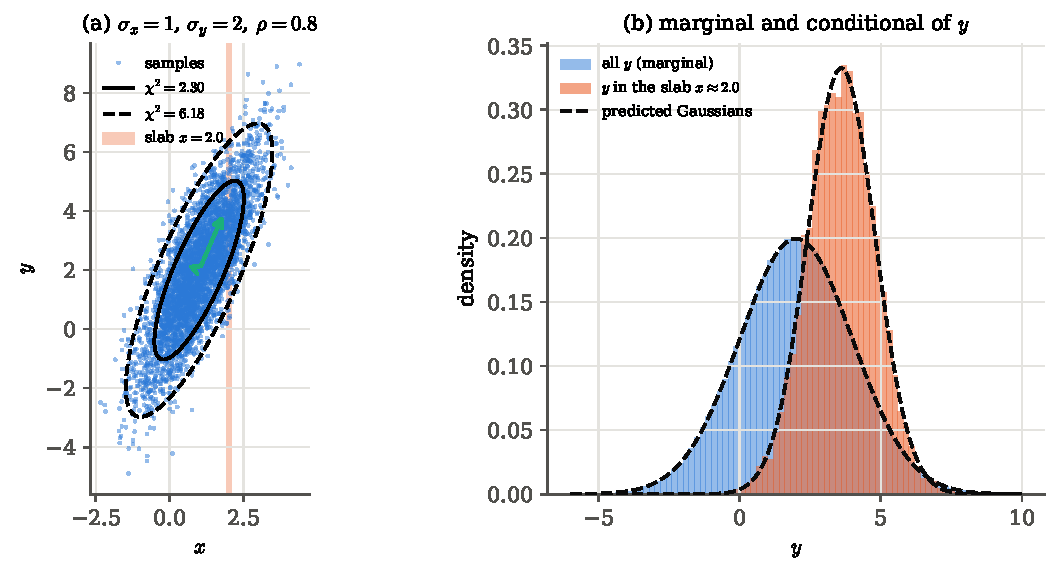
\includegraphics[width=\linewidth]{figures/ch02/mvn_ellipses.pdf}
\caption{(a) Samples of the bivariate Gaussian with $\sigma_x=1$, $\sigma_y=2$, $\rho=0.8$, with the $\Delta\chi^2=2.30$ and $6.18$ ellipses and the principal axes (arrows, of length one standard deviation along each axis). The shaded strip is the slab used for conditioning. (b) All $y$ values (the marginal) and the $y$ values inside the slab (the conditional), each with its predicted Gaussian. Fixing $x$ shifts the centre and shrinks the width.}
\label{2b:fig:mvn}
\end{figure}

\paragraph{The same object in three sciences.} The multivariate Gaussian is the common core of the three kinds of data this book keeps returning to. \emph{Colliders.} For Poisson counts in many bins it is the large-count limit of the product of Poissons. Its $\Cmat$ is diagonal, with variances equal to the means, until systematic uncertainties shared between bins add correlations. \emph{The CMB.} For a CMB map (\cref{ch:07}) the vector is the list of pixel temperatures or of the harmonic coefficients $\alm$, and $\Cmat$ is built from the power spectrum $\Cell$. For an isotropic Gaussian field the $\alm$ are independent with variance $\Cell$, so in harmonic space $\Cmat$ is diagonal. \emph{Gravitational waves.} For detector noise the vector is the time series and $\Cmat$ is set by the power spectral density. Stationarity makes it a Toeplitz matrix (constant along each diagonal), and the Fourier transform diagonalises it, just as the eigenbasis did in \eqref{2b:eq:mvn-ellipse}. In each case the step that makes the likelihood computable is the same: whiten, and then everything is a sum of independent squares. That sum of squares is the $\chi^2$ variable of \cref{2b:sec:chi2}. When the tails of real data are heavier than Gaussian, the multivariate Student-$t$, a Gaussian with a randomly rescaled covariance (\cref{2b:sec:t}), is the standard robust replacement \srcref{Lambert}{\S8.4.11}.
\section{Sums of squared Gaussians: the \texorpdfstring{$\chi^2$}{chi-squared} distribution}
\label{2b:sec:chi2}

We fit a straight line to ten points with error bars and get $\chi^2=\sum_i(x_i-\mu_i)^2/\sigma_i^2=14.2$, where $x_i$ is a measured value, $\mu_i$ the line's prediction and $\sigma_i$ the error bar. Is the fit good? The number means nothing until we know how $\chi^2$ is distributed when the model is right. Sums of squared Gaussians turn up throughout physics. A CMB band power $\Chat=\frac{1}{2\ell+1}\sum_m|\alm|^2$ is a sum of squares of Gaussian coefficients, and its scatter is cosmic variance. The power of Gaussian detector noise in one frequency bin of a gravitational-wave stream is the sum of two squares, the real and imaginary parts. The quadratic form in the exponent of the multivariate Gaussian, whose contours we just drew, is a sum of squares after whitening. And the sample variance of $n$ repeated measurements is a sum of squared deviations.

Two results answer these questions. A sum of $\nu$ squared standard normals has a definite distribution, $\chi^2_\nu$, with mean $\nu$ and variance $2\nu$. And the sample variance divides by $n-1$, not $n$, because estimating the mean uses up exactly one ``degree of freedom'' in a sense the geometry makes precise.

The questions, in words: \emph{if $\nu$ independent standard normal numbers are squared and added, what is the density of the total? And what changes when the numbers are deviations from their own average rather than from the true mean?}

\subsection{One square}
\label{2b:sec:chi2-one}

Start with a single square, $Q=Y^2$ with $Y\sim\Normal(0,1)$. \emph{When is $Q$ small?} For $q>0$, $Q\le q$ happens exactly when $-\sqrt q\le Y\le\sqrt q$. So we can get the density of $Q$ by differentiating the probability of that interval:
\begin{align}
  f_1(q)=\frac{\dd}{\dd q}\Prob(Q\le q)
  &\eqby{1} \frac{\dd}{\dd q}\bigl[\Phi(\sqrt q)-\Phi(-\sqrt q)\bigr]
   \eqby{2} 2\varphi(\sqrt q)\,\frac{1}{2\sqrt q}
   \eqby{3} \frac{1}{\sqrt{2\pi q}}\,e^{-q/2} .
  \label{2b:eq:chi2-one}
\end{align}
\begin{explain}
  \item The probability of an interval is the difference of the cumulative distribution at its ends.
  \item Chain rule, $\frac{\dd}{\dd q}\sqrt q=\frac1{2\sqrt q}$, and the symmetry $\varphi(-y)=\varphi(y)$. The two ends contribute equally: this is the factor two of \srcref{Cowan}{(10.14)}, which counts the positive and the negative root.
  \item $\varphi(\sqrt q)=e^{-q/2}/\sqrt{2\pi}$.
\end{explain}
The density diverges like $q^{-1/2}$ at the origin, because $Y$ is most likely near zero and squaring crowds those values towards $q=0$. One square is a gamma variable, Gamma$(\frac12,2)$ \srcref{CasellaBerger}{Lemma~5.3.2}. To check, recall the gamma density \eqref{2a:eq:gamma}: with shape $\alpha=\frac12$ and scale $\beta=2$ it is $q^{-1/2}e^{-q/2}/(\Gamma(\frac12)\sqrt2)$, and $\Gamma(\frac12)=\sqrt\pi$ \eqref{2b:eq:gamma-half} makes this identical to \eqref{2b:eq:chi2-one}.

\subsection{Many squares: two derivations}
\label{2b:sec:chi2-many}

\paragraph{The geometric route: integrate the joint density over a ball.} \emph{The question in words:} what is the probability that $Q_\nu\le q$, whatever the individual values of $Y_1,\dots,Y_\nu$ happen to be? We know the joint density of all the $Y_j$, and we do not care about them one by one, only about the one combination $Q_\nu$. So we do what we always do with variables we do not care about (\cref{1b:sec:marginal}): integrate the joint density over every set of values $y_1,\dots,y_\nu$ that gives $Q_\nu\le q$, and then change variables to $Q$. It goes in four steps.

\emph{Step 1: the joint density.} The $Y_j$ are independent, so their joint density is the product of the $\nu$ one-dimensional densities. Writing $\bm y=(y_1,\dots,y_\nu)$ and $|\bm y|^2=y_1^2+\dots+y_\nu^2$,
\begin{equation}
  f(\bm y)=\prod_{j=1}^{\nu}\frac{e^{-y_j^2/2}}{\sqrt{2\pi}}=\frac{e^{-(y_1^2+\dots+y_\nu^2)/2}}{(2\pi)^{\nu/2}}=\frac{e^{-|\bm y|^2/2}}{(2\pi)^{\nu/2}} ,
  \label{2b:eq:chi2-joint}
\end{equation}
since a product of exponentials is the exponential of the sum. The density depends on $\bm y$ only through its length $r=|\bm y|$: it is the same at every point of a sphere centred on the origin.

\emph{Step 2: the event $Q_\nu\le q$ is a ball.} $Q_\nu=|\bm Y|^2$ is the squared distance of the random point $\bm Y$ from the origin. So $Q_\nu\le q$ happens exactly when $\bm Y$ lands inside the ball of radius $\sqrt q$, and its probability is the joint density integrated over all $\bm y$ in that ball:
\[
  \Prob(Q_\nu\le q)=\int_{|\bm y|^2\le q}\frac{e^{-|\bm y|^2/2}}{(2\pi)^{\nu/2}}\,\dd^\nu y .
\]
This is the one-square argument of \cref{2b:sec:chi2-one} in $\nu$ dimensions: there the ball was the interval $[-\sqrt q,\sqrt q]$.

\emph{Step 3: spherical coordinates.} Because the integrand depends only on $r$, we slice the ball into thin spherical shells. A shell of radius $r$ and thickness $\dd r$ has volume $S_{\nu-1}r^{\nu-1}\dd r$, where $S_{\nu-1}$ is the area of the unit sphere in $\nu$ dimensions ($S_1=2\pi$, the circumference of the unit circle; $S_2=4\pi$). The power $r^{\nu-1}$ is there because a sphere of radius $r$ is the unit sphere stretched by $r$ in each of its $\nu-1$ directions. Integrating over the angles of each shell leaves a one-dimensional integral,
\begin{equation}
  \Prob(Q_\nu\le q)=\frac{S_{\nu-1}}{(2\pi)^{\nu/2}}\int_0^{\sqrt q}r^{\nu-1}e^{-r^2/2}\,\dd r .
  \label{2b:eq:chi2-ball}
\end{equation}
We still need $S_{\nu-1}$. The Gaussian integral gives it, by computing one integral in two ways. The integral of $e^{-|\bm y|^2/2}$ over all of $\mathbb R^\nu$ factorises into $\nu$ one-dimensional Gaussian integrals, each equal to $\sqrt{2\pi}$; in shells it is $S_{\nu-1}\int_0^\infty r^{\nu-1}e^{-r^2/2}\dd r$. Setting the two equal,
\begin{align}
  (2\pi)^{\nu/2}
  &\eqby{1} \int_{\mathbb R^\nu}e^{-|\bm y|^2/2}\,\dd^\nu y
   \eqby{2} S_{\nu-1}\int_0^\infty r^{\nu-1}e^{-r^2/2}\,\dd r
   \eqby{3} S_{\nu-1}\,2^{\nu/2-1}\,\Gamma\bigl(\tfrac\nu2\bigr)
  \quad\Longrightarrow\quad S_{\nu-1}=\frac{2\pi^{\nu/2}}{\Gamma(\nu/2)} .
  \label{2b:eq:sphere-area}
\end{align}
\begin{explain}
  \item Cartesian coordinates: $e^{-|\bm y|^2/2}=\prod_je^{-y_j^2/2}$, and each $\int_{-\infty}^\infty e^{-y_j^2/2}\dd y_j=\sqrt{2\pi}$.
  \item Spherical coordinates, as in step 3, with the ball extended to all of space.
  \item Substitute $t=r^2/2$, so $r=\sqrt{2t}$, $\dd r=\dd t/\sqrt{2t}$ and $r^{\nu-1}\dd r=(2t)^{\nu/2-1}\dd t$; the $t$ integral is $\int_0^\infty t^{\nu/2-1}e^{-t}\dd t=\Gamma(\nu/2)$.
\end{explain}
Divide by $2^{\nu/2-1}\Gamma(\nu/2)$ and use $(2\pi)^{\nu/2}/2^{\nu/2-1}=2\pi^{\nu/2}$. (Check: $\nu=2$ gives $2\pi/\Gamma(1)=2\pi$, and $\nu=3$ gives $2\pi^{3/2}/(\sqrt\pi/2)=4\pi$.)

\emph{Step 4: from the radius to $Q$, and differentiate.} In \eqref{2b:eq:chi2-ball} change the integration variable from $r$ to $s=r^2$, the value of $Q$ on the shell, and then differentiate with respect to the upper limit:
\begin{align}
  \Prob(Q_\nu\le q)
  &\eqby{1} \frac{S_{\nu-1}}{(2\pi)^{\nu/2}}\int_0^{q}s^{(\nu-1)/2}\,e^{-s/2}\,\frac{\dd s}{2\sqrt s}
   \eqby{2} \frac{1}{2^{\nu/2}\,\Gamma(\nu/2)}\int_0^{q}s^{\nu/2-1}\,e^{-s/2}\,\dd s ,
  \nonumber\\
  f_\nu(q)=\frac{\dd}{\dd q}\Prob(Q_\nu\le q)
  &\eqby{3} \frac{q^{\nu/2-1}e^{-q/2}}{2^{\nu/2}\,\Gamma(\nu/2)} ,\qquad q>0 ,
  \label{2b:eq:chi2}
\end{align}
\begin{explain}
  \item $r=\sqrt s$, so $r^{\nu-1}=s^{(\nu-1)/2}$ and $\dd r=\dd s/(2\sqrt s)$; the limits $r=0$ and $r=\sqrt q$ become $s=0$ and $s=q$.
  \item Insert $S_{\nu-1}$ from \eqref{2b:eq:sphere-area}: $\frac{2\pi^{\nu/2}}{\Gamma(\nu/2)}\cdot\frac{1}{(2\pi)^{\nu/2}}\cdot\frac12=\frac{1}{2^{\nu/2}\Gamma(\nu/2)}$, and combine the powers, $s^{(\nu-1)/2}s^{-1/2}=s^{\nu/2-1}$.
  \item The derivative of an integral with respect to its upper limit is the integrand at that limit.
\end{explain}
the $\chi^2$ density with $\nu$ \newterm{degrees of freedom} \srcref{Cowan}{(2.34)}, \mainref{p.~30}. The power $q^{\nu/2-1}$ is pure geometry: the area of a sphere of radius $\sqrt q$ in $\nu$ dimensions. In high dimensions this factor pushes the probability away from the origin, which is why $\chi^2_\nu$ peaks near $\nu-2$ rather than at zero. We use the same shell argument for the Maxwell--Boltzmann speed distribution in \cref{2b:sec:zoo}.

\paragraph{The characteristic function route.} The second route draws no sphere. Characteristic functions turn the sum of squares into a product \srcref{Cowan}{(10.12)--(10.15)}. First transform one square. With $a=1-2ik$,
\begin{align}
  \phi_1(k)=\E\,e^{ikY^2}
  &\eqby{1} \int_{-\infty}^{\infty}\frac{e^{-y^2/2}}{\sqrt{2\pi}}\,e^{iky^2}\,\dd y
   \eqby{2} \int_{-\infty}^{\infty}\frac{e^{-ay^2/2}}{\sqrt{2\pi}}\,\dd y
   \eqby{3} (1-2ik)^{-1/2} .
  \label{2b:eq:chi2-cf1}
\end{align}
\begin{explain}
  \item The expectation of a function of $Y$ is its integral against the density of $Y$.
  \item Combine the exponents: $-\frac{y^2}{2}+iky^2=-\frac{(1-2ik)y^2}{2}$.
  \item The Gaussian integral $\int e^{-ay^2/2}\dd y=\sqrt{2\pi/a}$, which holds for complex $a$ with positive real part (here $\mathrm{Re}\,a=1$) with the principal square root, by analytic continuation from real $a$.
\end{explain}
For $Q_\nu=Y_1^2+\dots+Y_\nu^2$ with independent $Y_j$, the product rule \eqref{2b:eq:cf-sum} gives $\phi_\nu(k)=(1-2ik)^{-\nu/2}$ \srcref{Cowan}{(10.15)}. Which density has this transform? One square was a gamma variable, so try the gamma density with shape $\alpha$ and scale $\beta$:
\begin{align}
  \int_0^\infty e^{ikx}\,\frac{x^{\alpha-1}e^{-x/\beta}}{\Gamma(\alpha)\beta^\alpha}\,\dd x
  &\eqby{1} \frac{1}{\Gamma(\alpha)\beta^\alpha}\int_0^\infty x^{\alpha-1}e^{-x(1-i\beta k)/\beta}\,\dd x
   \eqby{2} \frac{1}{\Gamma(\alpha)\beta^\alpha}\,\Gamma(\alpha)\Bigl(\frac{\beta}{1-i\beta k}\Bigr)^{\alpha}
   = (1-i\beta k)^{-\alpha} ,
  \label{2b:eq:gamma-cf}
\end{align}
\begin{explain}
  \item Combine the exponentials.
  \item Substitute $t=x(1-i\beta k)/\beta$; then $\int_0^\infty x^{\alpha-1}e^{-cx}\dd x=\Gamma(\alpha)/c^\alpha$, again valid for complex $c$ with positive real part.
\end{explain}
so $(1-2ik)^{-\nu/2}$ is the characteristic function of Gamma$(\nu/2,2)$. Since a characteristic function determines its density, $f_\nu(q)=q^{\nu/2-1}e^{-q/2}/(2^{\nu/2}\Gamma(\nu/2))$, which is \eqref{2b:eq:chi2} again: the product of $\nu$ transforms and the integral over a ball give the same density.

\begin{workdef}[$\chi^2$ distribution]
$Q\sim\chi^2_\nu$ if $Q=\sum_{j=1}^\nu Y_j^2$ with $Y_j\iid\Normal(0,1)$. Equivalently, $Q$ has density \eqref{2b:eq:chi2}, the Gamma$(\nu/2,2)$ density, and characteristic function $(1-2ik)^{-\nu/2}$.
\emph{Summary numbers:} $\E Q=\nu$, $\Var Q=2\nu$, mode $\max(\nu-2,0)$. \emph{Additivity:} independent $\chi^2_{\nu_1}$ and $\chi^2_{\nu_2}$ add to $\chi^2_{\nu_1+\nu_2}$ (multiply the characteristic functions).
\emph{Recognise it by:} a sum of squares of independent, zero-mean, unit-variance Gaussian quantities, such as residuals divided by their true errors.
\end{workdef}

\paragraph{Mean and variance.} The mean of $\chi^2_\nu$ is $\nu$ and its variance is $2\nu$. For one square, $\E Y^2=1$ and $\E Y^4=3$ (differentiate the Gaussian characteristic function four times, or integrate by parts twice as in \eqref{2b:eq:gauss-moments}), so $\Var Y^2=3-1=2$. Means and variances of independent terms add, so $\E Q_\nu=\nu$ and $\Var Q_\nu=2\nu$ \srcref{Cowan}{(2.36)--(2.37)}. The script sums $\nu$ squared normals $2\times10^5$ times and finds mean $\tbChiMeanFive$ and variance $\tbChiVarFive$ for $\nu=5$, and $\tbChiMeanTen$ and $\tbChiVarTen$ for $\nu=10$ (\cref{2b:fig:chi2-sums}a). For large $\nu$ the CLT makes $\chi^2_\nu\approx\Normal(\nu,2\nu)$, but slowly: its skewness is $\sqrt{8/\nu}$, still $0.28$ at $\nu=100$ (the skewness of one square, $\sqrt8$, shrinks like $1/\sqrt\nu$, as in \eqref{2b:eq:cumulant-scaling}).

\paragraph{Example: is $\chi^2=14.2$ for ten degrees of freedom a good fit?} Yes, it is acceptable. \emph{The question in words:} if the straight line is the right model, how often would a fit come out this bad or worse? With $\nu=10$, $\E\chi^2=10$ and the standard deviation is $\sqrt{20}=4.5$. So $14.2$ is less than one standard deviation high. Exactly, $\Prob(\chi^2_{10}>14.2)=0.16$: one fit in six would do this badly even with the right model. The central $90\%$ range of $\chi^2_{10}$ is $3.9$ to $18.3$. A fit with $\chi^2=24$ would have tail probability $0.008$ and would be suspicious.

The same reduced $\chi^2/\nu$ can mean different things for different $\nu$. Its standard deviation is $\sqrt{2/\nu}$, which is $0.45$ for ten points. So ``$\chi^2/\nu=1.4$'' is unremarkable for $\nu=10$, while for $\nu=100$ ($\chi^2=140$) it has tail probability $0.005$. Hypothesis tests built on this are the subject of \cref{ch:04}.

\paragraph{Example: cosmic variance.} A CMB band power is a $\chi^2$ variable, and that fixes its scatter. Recall that $\Chat=\frac{1}{2\ell+1}\sum_m|\alm|^2$ is the measured power at multipole $\ell$, built from the $2\ell+1$ harmonic coefficients $\alm$, and $\Cell$ is its true value. \emph{How many independent Gaussians go into it?} Exactly $2\ell+1$ real numbers. The $m=0$ coefficient is real. For $m>0$ the real and imaginary parts count separately. And $a_{\ell,-m}$ adds nothing new, being fixed by $a_{\ell,-m}=(-1)^ma^*_{\ell m}$. For an isotropic Gaussian sky these $2\ell+1$ numbers are independent Gaussians whose squares add up to $\sum_m|\alm|^2$, each with the same share of the variance. So $(2\ell+1)\Chat/\Cell\sim\chi^2_{2\ell+1}$, and
\[
  \Var\Chat\eqby{1}\Bigl(\frac{\Cell}{2\ell+1}\Bigr)^2\,\Var\chi^2_{2\ell+1}\eqby{2}\frac{\Cell^2}{(2\ell+1)^2}\,2(2\ell+1)=\frac{2\Cell^2}{2\ell+1},
\]
where (1) scales a random variable by a constant and (2) uses $\Var\chi^2_\nu=2\nu$. This is the cosmic variance that \cref{ch:07} verifies by simulation. At $\ell=2$, $\Chat$ is a $\chi^2_5$ variable divided by five: skewed, with a $1\sigma$ scatter of $63\%$.

\subsection{Correlated Gaussians: the quadratic form}
\label{2b:sec:chi2-quadform}

Correlations do not change the answer, as long as the sum of squares uses the full inverse covariance. If $\bm X\sim\Normal(\bm\mu,\Cmat)$ in $k$ dimensions, then
\begin{equation}
  Q=(\bm X-\bm\mu)\T\Cmat^{-1}(\bm X-\bm\mu)\ \sim\ \chi^2_k
  \label{2b:eq:quadform}
\end{equation}
\srcref{Cowan}{(2.39)}, \mainref{Thm~2.44(4)}. The proof is one line with the whitening of \cref{2b:sec:mvn}: with $\mathbf L$ the Cholesky factor, $\mathbf L\mathbf L\T=\Cmat$, the vector $\bm Z=\mathbf L^{-1}(\bm X-\bm\mu)$ has independent standard normal components and $\bm Z\T\bm Z=(\bm X-\bm\mu)\T(\mathbf L\mathbf L\T)^{-1}(\bm X-\bm\mu)=Q$. This is what justified the ellipse contents in \eqref{2b:eq:ellipse-content}.

\paragraph{Example: forgetting the correlations.} Dropping the off-diagonal elements keeps the right mean but gives the wrong spread. The script takes a correlated three-dimensional Gaussian with covariance
\[
  \Cmat=\begin{pmatrix}1&0.6&0.3\\0.6&2&-0.5\\0.3&-0.5&1.5\end{pmatrix}
\]
and computes $Q$ for $2\times10^5$ draws: mean $\tbQFmean$ and variance $\tbQFvar$, as $\chi^2_3$ requires. It also computes the ``naive'' sum $\sum_i(x_i-\mu_i)^2/C_{ii}$, which ignores the off-diagonal elements. Its mean is still $\tbNaiveMean$, because each term has expectation $1$ whatever the correlations. But its variance is $\tbNaiveVar$ instead of $6$ (\cref{2b:fig:chi2-sums}b), because the terms are correlated and so do not add like independent squares. A goodness-of-fit test that uses only the diagonal errors on correlated data (neighbouring bins of a smoothed spectrum, overlapping band powers) will reject correct models too often, even though its average looks fine.

\begin{figure}[htbp]
\centering
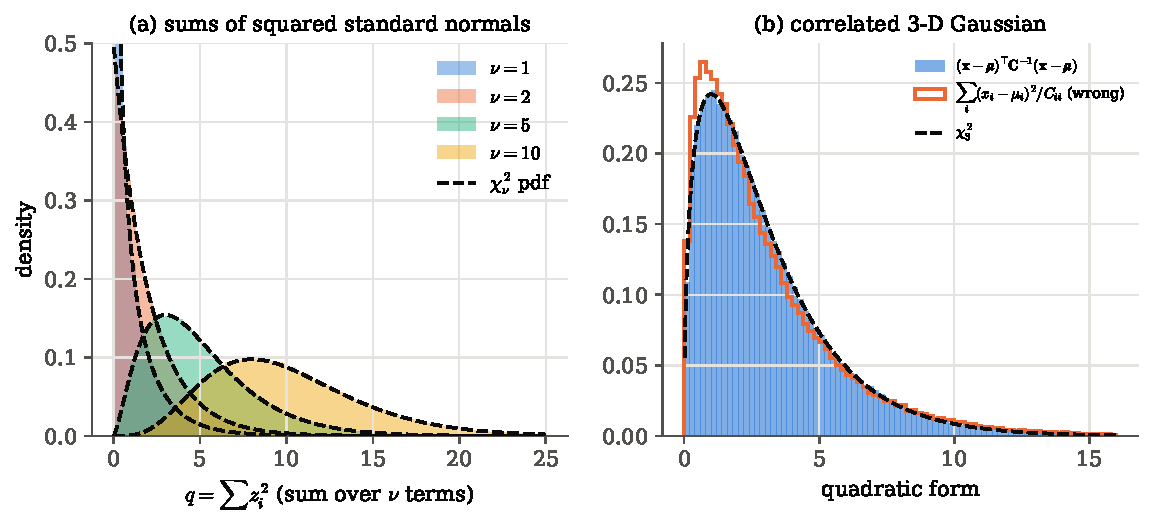
\includegraphics[width=\linewidth]{figures/ch02/chi2_sums.pdf}
\caption{(a) Histograms of sums of $\nu$ squared standard normals for $\nu=1,2,5,10$ against the $\chi^2_\nu$ densities (dashed). For $\nu=1$ and $2$ the density is largest at zero; for larger $\nu$ the peak moves out to $\nu-2$. (b) For a correlated three-dimensional Gaussian, the full quadratic form follows $\chi^2_3$, while the sum that uses only the diagonal variances (orange) has the right mean but the wrong shape: it piles up near zero and has a longer tail, so its variance is larger.}
\label{2b:fig:chi2-sums}
\end{figure}

\subsection{The sample variance and the lost degree of freedom}
\label{2b:sec:nminus1}

Five readings of a pendulum period, $x_1,\dots,x_5$, scatter about the unknown true value $\mu$ with unknown spread $\sigma$. We estimate $\mu$ by the sample mean $\bar x=\frac1n\sum x_i$, and $\sigma^2$ from the deviations $x_i-\bar x$. Why divide the sum of squared deviations by $n-1$?

\paragraph{The bias.} Deviations from $\bar x$ are systematically smaller than deviations from the true $\mu$. The reason: the sample mean is the value of $a$ that minimises $\sum_i(x_i-a)^2$ (set the derivative $-2\sum_i(x_i-a)$ to zero), so no other centre, $\mu$ included, gives a smaller sum. By how much smaller? Write $x_i-\mu=(x_i-\bar x)+(\bar x-\mu)$ and expand:
\begin{align}
  \sum_{i=1}^n(x_i-\mu)^2
  &\eqby{1} \sum_{i=1}^n(x_i-\bar x)^2+2(\bar x-\mu)\sum_{i=1}^n(x_i-\bar x)+n(\bar x-\mu)^2 \nonumber\\
  &\eqby{2} \sum_{i=1}^n(x_i-\bar x)^2+n(\bar x-\mu)^2 .
  \label{2b:eq:ss-split}
\end{align}
\begin{explain}
  \item Square the sum of two terms and sum over $i$; the last term does not depend on $i$.
  \item $\sum_i(x_i-\bar x)=n\bar x-n\bar x=0$.
\end{explain}
Take expectations for independent $x_i$ with variance $\sigma^2$, any distribution. The left side has expectation $n\sigma^2$ and $\E(\bar x-\mu)^2=\Var\bar x=\sigma^2/n$, so
\begin{equation}
  \E\sum_{i=1}^n(x_i-\bar x)^2=n\sigma^2-n\cdot\frac{\sigma^2}{n}=(n-1)\sigma^2 .
  \label{2b:eq:nminus1}
\end{equation}
Hence $S^2=\frac1{n-1}\sum(x_i-\bar x)^2$ has $\E S^2=\sigma^2$, while the ``natural'' $\frac1n\sum(x_i-\bar x)^2$ is low on average by the factor $(n-1)/n$. The script, with $n=\tbSVn$ and $\sigma^2=\tbSVsigmaSq$, finds $\E S^2=\tbSVmeanS$ and $\E\bigl[\frac1n\sum(x_i-\bar x)^2\bigr]=\tbSVmeanSn$, against the predicted $\tbSVbiasTh$. The missing $\sigma^2/n$ is exactly the variance of $\bar x$ around $\mu$: the part of the scatter that the sample mean ``absorbs'' by following the data.

\paragraph{The distribution: rotate the data.} For Gaussian data we can say much more: $(n-1)S^2/\sigma^2$ is exactly $\chi^2_{n-1}$, and it is independent of $\bar x$. A rotation of the data shows both. Picture the $n$ readings as one point $\bm x\in\R^n$. The sample mean is about the component of $\bm x$ along the diagonal direction $\bm e=(1,\dots,1)/\sqrt n$, since $\bm e\T\bm x=\sqrt n\,\bar x$. The deviations $x_i-\bar x$ are the components of what is left over, $\bm x-\sqrt n\,\bar x\,\bm e$, which is perpendicular to $\bm e$ and so lives in an $(n-1)$-dimensional subspace (\cref{2b:fig:helmert}). Choose an orthonormal basis whose first vector is $\bm e$, collect the basis vectors as the rows of an orthogonal matrix $\mathbf H$ (for $n=3$, one choice, the \newterm{Helmert} matrix, is shown below), and rotate: $\bm y=\mathbf H(\bm x-\mu\bm 1)$, where $\bm1=(1,\dots,1)$. Then:
\begin{itemize}
  \item $\bm x-\mu\bm1\sim\Normal(0,\sigma^2\Id)$, so by \eqref{2b:eq:mvn-linear} $\bm y\sim\Normal(0,\sigma^2\mathbf H\mathbf H\T)=\Normal(0,\sigma^2\Id)$: the $y_j$ are again independent with variance $\sigma^2$. An isotropic Gaussian looks the same in every rotated frame.
  \item $y_1=\bm e\T(\bm x-\mu\bm1)=\sqrt n(\bar x-\mu)$.
  \item A rotation preserves length, so $\sum_{j=1}^ny_j^2=\sum_i(x_i-\mu)^2$, and by \eqref{2b:eq:ss-split}, $\sum_{j=2}^ny_j^2=\sum_i(x_i-\mu)^2-n(\bar x-\mu)^2=\sum_i(x_i-\bar x)^2$.
\end{itemize}
The last line says that $(n-1)S^2/\sigma^2=\sum_{j=2}^n(y_j/\sigma)^2$ is a sum of $n-1$ independent squared standard normals, and it involves only $y_2,\dots,y_n$, which are independent of $y_1$ and hence of $\bar x$.

\paragraph{Example: $n=3$, by hand.} The rows of
\[
  \mathbf H=\begin{pmatrix}\tfrac1{\sqrt3}&\tfrac1{\sqrt3}&\tfrac1{\sqrt3}\\[2pt] \tfrac1{\sqrt2}&-\tfrac1{\sqrt2}&0\\[2pt] \tfrac1{\sqrt6}&\tfrac1{\sqrt6}&-\tfrac2{\sqrt6}\end{pmatrix}
\]
have unit length and are mutually orthogonal (for example, row 2 $\cdot$ row 3 $=\frac1{\sqrt{12}}-\frac1{\sqrt{12}}+0=0$). Take the readings $\bm x=(1,2,6)$, so $\bar x=3$ and $\sum(x_i-\bar x)^2=4+1+9=14$. The second and third rotated components (the shift by $\mu\bm1$ drops out of them, because their rows sum to zero) are $y_2=(1-2)/\sqrt2$ and $y_3=(1+2-12)/\sqrt6$, and $y_2^2+y_3^2=\frac12+\frac{81}6=14$. The first component carries the mean, the other two carry the scatter.

\begin{keyidea}[Sample mean and sample variance of Gaussian data]
If $x_1,\dots,x_n\iid\Normal(\mu,\sigma^2)$ \srcref{CasellaBerger}{Thm~5.3.1}:
(a) $\bar x$ and $S^2$ are independent;
(b) $\bar x\sim\Normal(\mu,\sigma^2/n)$;
(c) $(n-1)S^2/\sigma^2\sim\chi^2_{n-1}$.
One degree of freedom is spent on the direction along which $\bar x$ is measured; the scatter lives in the remaining $n-1$.
\end{keyidea}

Casella and Berger prove (a) by factorising the joint density after the change of variables $(\bar x,x_2-\bar x,\dots,x_n-\bar x)$, and (c) by induction, adding one data point at a time with the update $(n-1)S_n^2=(n-2)S_{n-1}^2+\frac{n-1}{n}(x_n-\bar x_{n-1})^2$ \srcref{CasellaBerger}{(5.3.1)--(5.3.2)}. They also give the fastest check of (a): $\Cov(\bar x,x_j-\bar x)=\sum_i\frac1n(\delta_{ij}-\frac1n)\sigma^2=0$, and uncorrelated linear functions of independent Gaussians are independent \srcref{CasellaBerger}{Lemma~5.3.3}. The rotation is the same argument seen geometrically.

\begin{figure}[htbp]
\centering
\begin{tikzpicture}[scale=0.95]
  \draw[faint,->] (-0.4,0) -- (4.6,0) node[anchor=north,lbl] {$x_1-\mu$};
  \draw[faint,->] (0,-0.4) -- (0,4.4) node[anchor=east,lbl] {$x_2-\mu$};
  \draw[formblue,thick] (-0.3,-0.3) -- (4.2,4.2);
  \node[lbl,formblue,anchor=west] at (4.2,4.2) {direction $\bm e=(1,1)/\sqrt2$};
  \coordinate (X) at (1.2,3.6);
  \coordinate (P) at (2.4,2.4); %
  \fill (X) circle (1.6pt);
  \node[lbl,anchor=east] at (1.1,3.7) {data $\bm x$};
  \fill[formblue] (P) circle (1.6pt);
  \node[lbl,anchor=north west,formblue] at (2.5,2.35) {$(\bar x,\bar x)$};
  \draw[bdryred,very thick] (P) -- (X);
  \node[lbl,bdryred,anchor=south west] at (1.95,3.05) {residual};
  \draw[thin] ($(P)+(-0.18,0.18)$) -- ($(P)+(0,0.36)$) -- ($(P)+(0.18,0.18)$);
  \draw[bdryred!50,dashed] (0.6,4.2) -- (4.2,0.6);
\end{tikzpicture}
\caption{Two readings seen as one point $\bm x$ in the plane (origin at the true value). Projecting onto the diagonal gives the sample mean $(\bar x,\bar x)$; the residual, whose length squared is $\sum(x_i-\bar x)^2$, is perpendicular to the diagonal. All data sets with the same mean lie on the dashed line, so the residual has only $n-1=1$ direction to move in. For an isotropic Gaussian the component along the diagonal and the component across it are independent.}
\label{2b:fig:helmert}
\end{figure}

\paragraph{Python: checking the theorem, and seeing it fail.} The script draws $\tbSVnrep$ samples of $n=\tbSVn$ Gaussian readings.

\pyfile[firstline=67,lastline=80,firstnumber=67]{code/ch02/25_chi2_sampvar.py}{The sample variance: $n-1$ degrees of freedom, and independence from the mean}

Line 70 computes $S^2$ with \pyname{ddof=1}, numpy's name for dividing by $n-1$ (``delta degrees of freedom''). Line 71 divides by $n$. Line 72 forms $(n-1)S^2/\sigma^2$, whose simulated mean and variance are $\tbSVwMean$ and $\tbSVwVar$, as $\chi^2_4$ requires ($4$ and $8$). Line 75 forms the same sum with the true mean instead of $\bar x$, which follows $\chi^2_5$ instead (\cref{2b:fig:chi2-sampvar}a). Lines 78--80 test independence, and show where it fails. The correlation between $\bar x$ and $S^2$ is $\tbSVcorrGauss$ for Gaussian readings, but $\tbSVcorrExp$ for exponential readings. \emph{Why?} For a skewed parent, a sample that happens to contain a large value has both a large mean and a large variance. The independence of $\bar x$ and $S^2$ is special to the Gaussian (it actually characterises it), and so is everything built on it in the next section.

\begin{figure}[htbp]
\centering
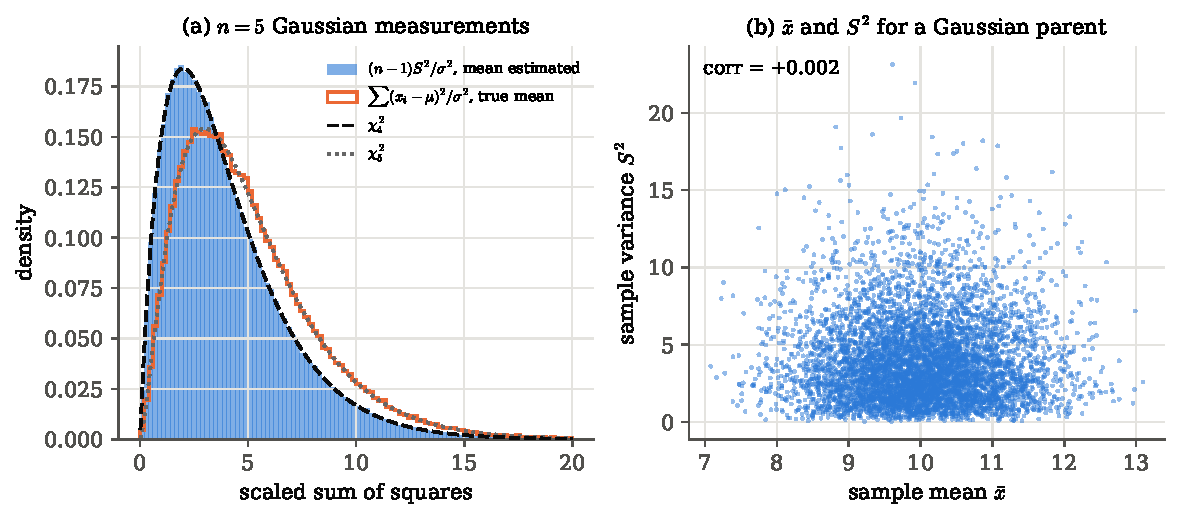
\includegraphics[width=\linewidth]{figures/ch02/chi2_sampvar.pdf}
\caption{(a) For five Gaussian readings, the scaled sum of squared deviations from the sample mean (histogram) follows $\chi^2_4$ (dashed), while deviations from the true mean (outline) follow $\chi^2_5$ (dotted). (b) Sample mean against sample variance for Gaussian readings: no trend at all, as independence requires.}
\label{2b:fig:chi2-sampvar}
\end{figure}

\begin{pitfall}[Degrees of freedom are dimensions, not data points]
The rule ``$\nu$ = number of data minus number of fitted parameters'' is the rotation argument again: each parameter that enters the model \emph{linearly} and is fitted by least squares removes one direction from the residual vector, exactly as $\bar x$ did. The rule is exact for linear models with Gaussian errors, approximate for nonlinear ones, and wrong when the data are correlated but treated as independent, or when parameters sit at a physical boundary.
\end{pitfall}
\section{When the error bar is itself estimated: Student's \texorpdfstring{$t$}{t} and the \texorpdfstring{$F$}{F} ratio}
\label{2b:sec:t}

We time five swings of a pendulum, compute $g$ from each, and quote the result as $\bar x\pm S/\sqrt5$, with $S$ the sample standard deviation. Then, to claim a ``two-sigma'' discrepancy with the textbook value, we check whether $|\bar x-g_0|$ exceeds $1.96\,S/\sqrt5$. This is wrong, and not by a little. The rule $1.96$ comes from the Gaussian, and it assumes that we know the true $\sigma$. We do not. Our error bar is itself a random number, computed from the same five readings, and sometimes it comes out much too small. When it does, the ratio $(\bar x-\mu)/(S/\sqrt n)$ is large, with $\mu$ the true value. So the ratio has fatter tails than a Gaussian. W.~S.~Gosset, who faced exactly this with small samples at the Guinness brewery and published as ``Student'', derived its distribution \srcref{CasellaBerger}{p.~181}.

Gosset's distribution does three jobs. It is the exact distribution of the \emph{studentised} mean for Gaussian data, so small-sample intervals and tests built on it are honest. It is also a Gaussian whose variance is itself random, which makes it the standard robust replacement for a Gaussian likelihood. And the same construction applied to two variances gives the $F$ distribution, the tool for asking whether two detectors, two runs or two models have the same scatter.

The question, in words: \emph{if a Gaussian quantity is divided by an independent, estimated measure of its own spread, how is the ratio distributed, and how different is it from a Gaussian?}

\subsection{The studentised mean}
\label{2b:sec:t-derive}

\emph{Why this ratio appears.} Let $x_1,\dots,x_n\iid\Normal(\mu,\sigma^2)$. If we
knew $\sigma$, the standardised mean
\begin{equation*}
  U=\frac{\bar x-\mu}{\sigma/\sqrt n}\sim\Normal(0,1)
\end{equation*}
would be all we need. We do not know $\sigma$, so we replace it by the sample
standard deviation $S$, with $S^2=\frac1{n-1}\sum_i(x_i-\bar x)^2$. Write $p=n-1$.
The quantity we actually compute is the \newterm{studentised mean}, and dividing its
top and bottom by $\sigma/\sqrt n$ shows what it is made of
\srcref{CasellaBerger}{(5.3.5)}:
\begin{align}
  T=\frac{\bar x-\mu}{S/\sqrt n}
  &\eqby{1} \frac{(\bar x-\mu)/(\sigma/\sqrt n)}{\sqrt{S^2/\sigma^2}}
   \eqby{2} \frac{U}{\sqrt{V/p}},
  \qquad V=\frac{(n-1)S^2}{\sigma^2}\sim\chi^2_p .
  \label{2b:eq:t-ratio}
\end{align}
\begin{explain}
  \item Divide numerator and denominator by $\sigma/\sqrt n$. The $\sqrt n$ cancels in the denominator.
  \item $S^2/\sigma^2=V/p$ by the definition of $V$. That $V$ is $\chi^2_p$, and that $U$ and $V$ are independent, are the results on the sample mean and variance of \cref{2b:sec:nminus1}.
\end{explain}
The unknown $\sigma$ has cancelled. So the whole problem is: given two independent
pieces, $U\sim\Normal(0,1)$ and $V\sim\chi^2_p$, what is the distribution of
$T=U/\sqrt{V/p}$?

\emph{The two ingredients and their joint density.} The density of $U$ is the standard
Gaussian, and the density of $V$ is the $\chi^2_p$ density \eqref{2b:eq:chi2}:
\begin{equation}
  f_U(u)=\frac{1}{\sqrt{2\pi}}\,e^{-u^2/2},
  \qquad
  f_V(v)=\frac{1}{2^{p/2}\Gamma(p/2)}\,v^{p/2-1}e^{-v/2}\quad(v>0).
  \label{2b:eq:t-ingredients}
\end{equation}
Because $U$ and $V$ are independent, their joint density is the product,
$f_{U,V}(u,v)=f_U(u)\,f_V(v)$.

\emph{Change variables from $(U,V)$ to $(T,V)$.} We keep $V$ and trade $U$ for $T$.
Solving \eqref{2b:eq:t-ratio} for $u$ gives the map and its Jacobian:
\begin{align}
  u=t\sqrt{\frac vp},\quad v=v,
  \qquad
  \left|\frac{\partial(u,v)}{\partial(t,v)}\right|
  &\eqby{1} \left|\begin{matrix}\sqrt{v/p} & \dfrac{t}{2\sqrt{pv}}\\[6pt] 0 & 1\end{matrix}\right|
   \eqby{2} \sqrt{\frac vp}.
  \label{2b:eq:t-jacobian}
\end{align}
\begin{explain}
  \item The four partial derivatives: $\partial u/\partial t=\sqrt{v/p}$, $\partial u/\partial v=t/(2\sqrt{pv})$, $\partial v/\partial t=0$, $\partial v/\partial v=1$.
  \item The matrix is triangular, so its determinant is the product of the diagonal entries. The off-diagonal entry never matters.
\end{explain}
The joint density of $(T,V)$ is the old joint density, evaluated at the old variables,
times this Jacobian (the rule of \cref{1b:eq:jacobian-2d}):
\begin{align}
  f_{T,V}(t,v)
  &\eqby{1} f_U\!\Bigl(t\sqrt{\tfrac vp}\Bigr)\,f_V(v)\,\sqrt{\frac vp} \nonumber\\
  &\eqby{2} \frac{1}{\sqrt{2\pi}}e^{-t^2v/(2p)}\;
            \frac{v^{p/2-1}e^{-v/2}}{2^{p/2}\Gamma(p/2)}\;\sqrt{\frac vp} \nonumber\\
  &\eqby{3} \frac{1}{\sqrt{2\pi p}\;2^{p/2}\Gamma(p/2)}\;
            v^{(p+1)/2-1}\,
            \exp\!\Bigl[-\frac v2\Bigl(1+\frac{t^2}{p}\Bigr)\Bigr].
  \label{2b:eq:t-joint}
\end{align}
\begin{explain}
  \item Change of variables, with the joint density of $(U,V)$ factorised by independence.
  \item Substitute the two densities \eqref{2b:eq:t-ingredients}, with $u^2=t^2v/p$.
  \item Collect the powers of $v$: $v^{p/2-1}\cdot v^{1/2}=v^{(p+1)/2-1}$. Collect the exponentials: $e^{-t^2v/(2p)}\,e^{-v/2}=e^{-\frac v2(1+t^2/p)}$. The constants are $1/\sqrt{2\pi}$, $1/\sqrt p$ and $1/(2^{p/2}\Gamma(p/2))$.
\end{explain}

\emph{The question that finishes the job.} What is the probability density for $T=t$,
regardless of what $V$ happens to be? That is a marginal density: we have the joint
density of $(T,V)$, and $V$ is a nuisance we do not care about, so we integrate it out
(\cref{1b:sec:marginal}). Write $A=1+t^2/p$ to keep the formula short. Then
\begin{align}
  f_T(t)
  &\eqby{1} \int_0^\infty f_{T,V}(t,v)\,\dd v \nonumber\\
  &\eqby{2} \frac{1}{\sqrt{2\pi p}\;2^{p/2}\Gamma(p/2)}
            \int_0^\infty v^{(p+1)/2-1}\,e^{-Av/2}\,\dd v \nonumber\\
  &\eqby{3} \frac{1}{\sqrt{2\pi p}\;2^{p/2}\Gamma(p/2)}\;
            \Gamma\Bigl(\frac{p+1}{2}\Bigr)\Bigl(\frac{2}{A}\Bigr)^{(p+1)/2} \nonumber\\
  &\eqby{4} \frac{\Gamma\bigl(\frac{p+1}{2}\bigr)}{\Gamma\bigl(\frac p2\bigr)\sqrt{p\pi}}\;
            \Bigl(1+\frac{t^2}{p}\Bigr)^{-(p+1)/2} .
  \label{2b:eq:student}
\end{align}
\begin{explain}
  \item Marginalisation: the density of $T$ alone is the joint density summed (integrated) over every value $V$ can take.
  \item Insert \eqref{2b:eq:t-joint}. Everything that does not depend on $v$ comes outside the integral.
  \item The gamma integral $\int_0^\infty x^{a-1}e^{-bx}\,\dd x=\Gamma(a)/b^a$, with $a=\frac{p+1}{2}$ and $b=\frac A2$, so $1/b^a=(2/A)^{(p+1)/2}$.
  \item The powers of two cancel, $2^{(p+1)/2}/(2^{p/2}\sqrt2)=1$, leaving $1/\sqrt{\pi p}$; then put back $A=1+t^2/p$.
\end{explain}
This is Student's $t$ density with $p$ degrees of freedom \srcref{CasellaBerger}{(5.3.6)}, \mainref{p.~30}.
The whole construction fits in one line: a standard Gaussian $U$, divided by the
square root of an independent $\chi^2_p/p$, is $t_p$. The $t$ distribution exists because
the fixed $\sigma$ of a Gaussian standardisation has been replaced by a random estimate,
whose square is a scaled $\chi^2$, and that extra randomness fattens the tails.

\begin{workdef}[Student's $t$ distribution]
$T\sim t_p$ if $T=U/\sqrt{V/p}$ with $U\sim\Normal(0,1)$ and $V\sim\chi^2_p$ independent; its density is \eqref{2b:eq:student}. For Gaussian data, $(\bar x-\mu)/(S/\sqrt n)\sim t_{n-1}$ exactly, for every $n\ge2$.
\emph{Equivalent picture:} a Gaussian $\Normal(0,\sigma^2)$ whose variance is random, $\sigma^2\sim$ Inv-Gamma$(p/2,p/2)$ \unpack{so the precision $1/\sigma^2$ is a gamma variable with mean one} \srcref{Lambert}{\S8.4.7}.
\emph{Summary numbers:} $\E T=0$ for $p>1$, $\Var T=p/(p-2)$ for $p>2$; only moments of order less than $p$ exist.
\end{workdef}

\paragraph{The tails, and the moments that do not exist.} For large $|t|$, \eqref{2b:eq:student} falls like $|t|^{-(p+1)}$, a power law. So $\E|T|^r$ is finite only for $r<p$ \srcref{CasellaBerger}{(5.3.7)}. With $p=1$ the density is $\Gamma(1)/(\Gamma(\frac12)\sqrt\pi)\,(1+t^2)^{-1}=\frac{1}{\pi(1+t^2)}$, the Cauchy distribution of \cref{2b:sec:cauchy}. So the studentised mean of \emph{two} Gaussian measurements has no mean at all. The variance, for $p>2$, follows from independence:
\begin{align}
  \Var T=\E T^2
  &\eqby{1} p\,\E(U^2)\,\E\Bigl(\frac1V\Bigr)
   \eqby{2} p\int_0^\infty\frac1v\,\frac{v^{p/2-1}e^{-v/2}}{2^{p/2}\Gamma(p/2)}\,\dd v
   \eqby{3} p\,\frac{2^{p/2-1}\Gamma(p/2-1)}{2^{p/2}\Gamma(p/2)}
   \eqby{4} \frac{p}{p-2} .
  \label{2b:eq:t-var}
\end{align}
\begin{explain}
  \item $T^2=pU^2/V$ with $U$ and $V$ independent, so the expectation factorises; $\E T=0$ by symmetry.
  \item $\E U^2=1$, and the expectation of $1/V$ is its integral against the $\chi^2_p$ density.
  \item The integrand is $v^{(p/2-1)-1}e^{-v/2}$, which integrates to $\Gamma(p/2-1)\,2^{p/2-1}$ provided $p>2$ (otherwise it diverges at $v=0$).
  \item $\Gamma(p/2)=(p/2-1)\Gamma(p/2-1)$, so the ratio is $\frac{1}{2(p/2-1)}=\frac1{p-2}$.
\end{explain}
The variance of $T$ is dominated by the rare samples whose estimated error bar $S$ happens to be tiny. That is what the divergence of step (3) at small $v$ means. As $p\to\infty$, $V/p\to1$ by the law of large numbers and $(1+t^2/p)^{-(p+1)/2}\to e^{-t^2/2}$, so $t_\infty=\Normal(0,1)$ \mainref{p.~30}. For non-Gaussian data and large $n$ the studentised mean still tends to $\Normal(0,1)$ (the studentised CLT, \mainref{Thm~5.10}). What the $t$ distribution adds is the \emph{exact} small-$n$ answer for Gaussian data.

\paragraph{Example: five pendulum readings.} Back to the five pendulum values of $g$ from the opening: how often does the Gaussian rule cry ``two sigma'' when nothing is wrong? The script simulates $\tbTnrep$ experiments of $n=\tbTn$ readings with $\sigma=0.05$\,m\,s$^{-2}$ and computes $T$ for each.

\pyfile[firstline=35,lastline=46,firstnumber=35]{code/ch02/26_student_t_F.py}{The studentised mean of five Gaussian readings}

Line 38 estimates the error bar from the same five numbers (\pyname{ddof=1} is the $n-1$ divisor). Line 39 forms $T$ with the estimated error bar and line 40 forms the same ratio with the true $\sigma$, which is exactly $\Normal(0,1)$. Lines 42--46 count how often each exceeds various thresholds. \emph{With the true $\sigma$}, $|Z|>1.96$ happens in a fraction $\tbZfracOneNineSix$ of experiments, the promised $5\%$. \emph{With the estimated error bar}, $|T|>1.96$ happens in $\tbTfracOneNineSix$, against the $t_4$ prediction $\tbTfracOneNineSixTh$. So the nominal ``$2\sigma$ discrepancy'' occurs more than twice as often as claimed. The correct $95\%$ point is $t_{4,\,0.975}=\tbTquant$, and $|T|$ exceeds it in a fraction $\tbTfracQuant$. Further out the difference explodes: $|T|>3$ happens in $\tbTfracThree$ of experiments ($t_4$: $\tbTfracThreeTh$), fifteen times the Gaussian $\tbTfracThreeGauss$ (\cref{2b:fig:t}a).

\begin{pitfall}[Do not use Gaussian thresholds with an estimated error bar]
With $n$ readings and $\sigma$ estimated from them, the two-sided $95\%$ multiplier is $t_{n-1,0.975}$: $12.7$ for $n=2$, $4.30$ for $n=3$, $2.78$ for $n=5$, $2.26$ for $n=10$, $2.09$ for $n=20$, and it reaches $1.96$ only as $n\to\infty$. For three-sigma or five-sigma claims the Gaussian rule is off by orders of magnitude unless $n$ is large. And the exact $t$ needs Gaussian readings: with a few outliers even $t$ is too optimistic.
\end{pitfall}

\paragraph{Example: a Gaussian with a random width.} Integrating $V$ out of \eqref{2b:eq:t-joint} has a second reading. For a fixed value $V=v$, $T=U\sqrt{p/v}$ is just a Gaussian with variance $p/v$; integrating over $v$ averages these Gaussians of different widths. So the $t$ distribution is a Gaussian whose width is itself random, and that is also a recipe for modelling data. Lambert's schools example \srcref{Lambert}{\S8.4.7} merges the test scores of many schools that share one mean but have different spreads. Each school on its own is Gaussian; the merged population is not. If the school variances are distributed as $\sigma^2\sim$ Inv-Gamma$(\nu/2,\nu/2)$, equivalently the precisions $1/\sigma^2$ as Gamma$(\nu/2,\text{scale }2/\nu)$, which is $\chi^2_\nu/\nu$, the merged distribution is exactly $t_\nu$: ``its head rises, its shoulders fall, and its tails fatten.'' The script draws $\tbTnrep$ values both ways for $\nu=\tbTmixNu$: as a Gaussian with a random precision (lines 51--52), and as $U/\sqrt{V/\nu}$ (line 54). Both histograms follow $t_3$, with Kolmogorov--Smirnov distances \unpack{the largest gap between the empirical and the exact cumulative distribution} of $\tbTksMix$ and $\tbTksUV$, as small as sampling noise allows at this sample size (\cref{2b:fig:t}b).

So the $t$ distribution is the workhorse \emph{robust likelihood}. When a few measurements have underestimated errors, when a detector occasionally misbehaves, when the population is heterogeneous, a $t_\nu$ likelihood with $\nu$ of a few lets outliers exist without dragging the fit. The degrees of freedom need not be an integer: $\nu$ is a free, real-valued shape parameter that can itself be fitted \srcref{Lambert}{\S8.4.7}. Its multivariate version, a multivariate Gaussian with one random scale factor for the whole covariance, gives joint tails heavy enough to see Lambert's hedge-fund ``bankruptcy days'' that a multivariate normal fit misses \srcref{Lambert}{\S8.4.11}.

\begin{figure}[htbp]
\centering
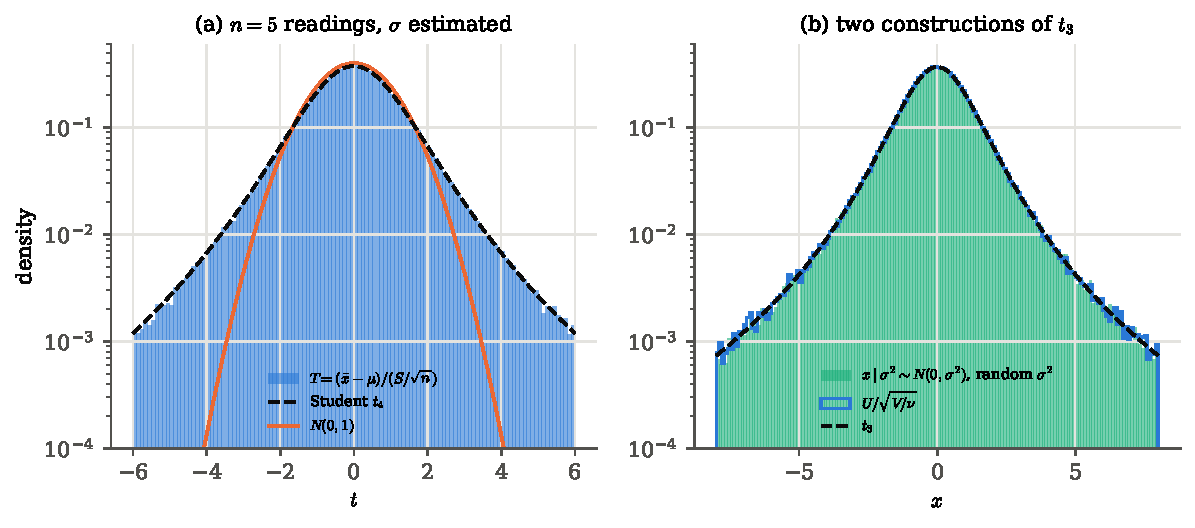
\includegraphics[width=\linewidth]{figures/ch02/t_student.pdf}
\caption{(a) The studentised mean of five Gaussian readings (histogram, logarithmic scale) follows Student's $t_4$ (dashed). The standard normal (solid) is far too thin in the tails. (b) Two constructions of $t_3$: a Gaussian whose variance is drawn afresh from an inverse-gamma distribution for every value, and the ratio $U/\sqrt{V/\nu}$. They are the same distribution.}
\label{2b:fig:t}
\end{figure}

\subsection{Ratios of variances: Snedecor's \texorpdfstring{$F$}{F}}
\label{2b:sec:F}

Two calorimeters measure the same electron beam. Calorimeter $X$ gives $n_X$ readings with sample variance $S_X^2$, calorimeter $Y$ gives $n_Y$ readings with $S_Y^2$. Is $X$'s resolution really worse, or did the numbers fluctuate? For Gaussian readings each $(n-1)S^2/\sigma^2$ is $\chi^2_{n-1}$, and the two are independent, so \srcref{CasellaBerger}{(5.3.8)}
\begin{equation}
  F=\frac{S_X^2/\sigma_X^2}{S_Y^2/\sigma_Y^2}=\frac{V_1/p}{V_2/q},\qquad V_1\sim\chi^2_p,\quad V_2\sim\chi^2_q,\qquad p=n_X-1,\quad q=n_Y-1 .
  \label{2b:eq:F-ratio}
\end{equation}
Under the hypothesis $\sigma_X=\sigma_Y$ the unknown widths cancel and $F=S_X^2/S_Y^2$ is computable from the data. Its density comes from the same trick as for $t$: hold the denominator fixed, then average over it. Fix $V_2=w$. Then $F=\frac{q}{pw}V_1$, so $V_1=\frac{pw}{q}x$ and $f_{F\given w}(x)=\frac{pw}{q}f_p\bigl(\frac{pwx}{q}\bigr)$. Averaging over $w$:
\begin{align}
  f_F(x)
  &\eqby{1} \int_0^\infty f_q(w)\,\frac{pw}{q}\,f_p\Bigl(\frac{pwx}{q}\Bigr)\dd w \nonumber\\
  &\eqby{2} \frac{(p/q)^{p/2}\,x^{p/2-1}}{2^{(p+q)/2}\Gamma(\frac p2)\Gamma(\frac q2)}\int_0^\infty w^{(p+q)/2-1}\,e^{-\frac w2\left(1+\frac{px}{q}\right)}\dd w \nonumber\\
  &\eqby{3} \frac{\Gamma\bigl(\frac{p+q}{2}\bigr)}{\Gamma\bigl(\frac p2\bigr)\Gamma\bigl(\frac q2\bigr)}\Bigl(\frac pq\Bigr)^{p/2}\frac{x^{p/2-1}}{\bigl(1+\frac pq x\bigr)^{(p+q)/2}},\qquad x>0 .
  \label{2b:eq:F}
\end{align}
\begin{explain}
  \item Law of total probability, with the change-of-variable factor $\frac{\dd V_1}{\dd x}=\frac{pw}{q}$.
  \item Insert both $\chi^2$ densities \eqref{2b:eq:chi2}. The powers of $w$ are $1+(\frac p2-1)+(\frac q2-1)=\frac{p+q}2-1$; the $x$-dependence outside the integral is $x^{p/2-1}$ with the constant $(p/q)^{1+p/2-1}$.
  \item The gamma integral with $a=\frac{p+q}{2}$ and $c=\frac12(1+px/q)$; the factor $2^{(p+q)/2}$ cancels.
\end{explain}
This is Snedecor's $F_{p,q}$ density \srcref{CasellaBerger}{(5.3.9)}. Its mean is slightly above one. By the same factorisation as \eqref{2b:eq:t-var}, $\E F=\frac qp\,\E V_1\,\E\frac1{V_2}=\frac{q}{q-2}$ for $q>2$ \srcref{CasellaBerger}{Ex.~5.3.7}. It exceeds one because $1/V_2$ is convex, so its average exceeds one over the average of $V_2$.

Three facts connect $F$ to its neighbours \srcref{CasellaBerger}{Thm~5.3.8}, and each is visible from the definition \eqref{2b:eq:F-ratio}. First, $1/F\sim F_{q,p}$: swap numerator and denominator. Second, if $T\sim t_q$ then $T^2=U^2/(V/q)=(\chi^2_1/1)/(\chi^2_q/q)\sim F_{1,q}$. Third, $\frac{(p/q)F}{1+(p/q)F}=\frac{V_1}{V_1+V_2}\sim$ Beta$(p/2,q/2)$, the fraction of a total carried by one gamma variable, which we derive in \cref{2b:sec:zoo}. Casella and Berger also note Kelker's result: the ratio has an $F$ distribution for any spherically symmetric parent, not only the Gaussian. So the $F$ test is somewhat robust.

\paragraph{Example: two calorimeters.} Small samples determine variances poorly. With six and eleven readings, one calorimeter's variance must come out more than three times the other's before we can claim, at the $5\%$ level, that its resolution is worse. The script shows this. It takes $n_X=6$ readings with $\sigma_X=1.5$ and $n_Y=11$ readings with $\sigma_Y=0.4$ (the true widths differ, but they cancel in \eqref{2b:eq:F-ratio}), so $p=\tbFdOne$ and $q=\tbFdTwo$. Over $\tbTnrep$ repetitions the mean of $F$ is $\tbFmean$, against $q/(q-2)=\tbFmeanTh$. The $95$th percentile of $F_{5,10}$ is $\tbFninetyfive$, and it is exceeded in a fraction $\tbFfracNinetyfive$ of repetitions (\cref{2b:fig:F}a). The script also squares the $t_4$ values of the pendulum experiment and compares them with $F_{1,4}$: the Kolmogorov--Smirnov distance on $10^5$ values is $\tbFksTsq$ (\cref{2b:fig:F}b).

\begin{figure}[htbp]
\centering
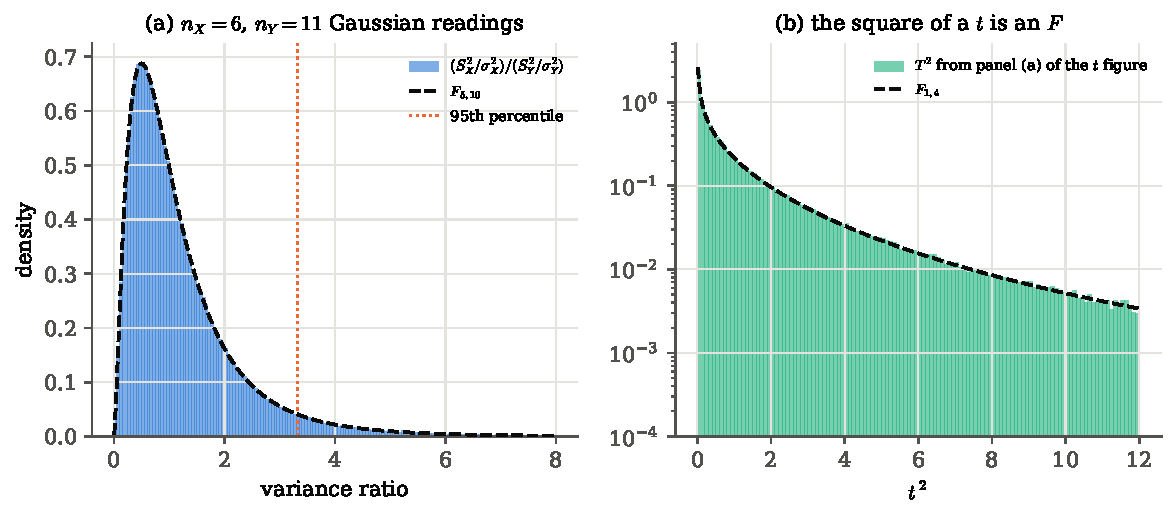
\includegraphics[width=\linewidth]{figures/ch02/f_ratio.pdf}
\caption{(a) The ratio of two scaled sample variances, from six and eleven Gaussian readings, follows $F_{5,10}$ (dashed); the dotted line marks its 95th percentile. (b) The squares of the studentised means of the pendulum experiment follow $F_{1,4}$, on a logarithmic scale that shows the power-law tail.}
\label{2b:fig:F}
\end{figure}

\paragraph{Where the ratios come back.} Every exact small-sample test in classical statistics is built on one pattern: a Gaussian or a $\chi^2$, divided by an independent $\chi^2$ that estimates the unknown scale. Examples are the $t$ test for a mean, the two-sample $t$ test, the $F$ test for the equality of variances, and the $F$ test that compares a model with a nested model having extra parameters by the ratio of $\chi^2$ improvements. These are the subject of \cref{ch:04}. Bayesian inference (\cref{ch:05}) arrives at the same $t_{n-1}$. Integrating an unknown Gaussian $\sigma$ out of the posterior for $\mu$, with the prior $p(\sigma)\propto1/\sigma$, produces it \srcref{Sivia}{p.~56--57, (3.43)--(3.44)}. The fattening of the tails is the price of not knowing the noise level, whichever school of inference pays it.
\section{The rest of the zoo, each with the machine that makes it}
\label{2b:sec:zoo}

Almost every distribution a physicist meets is produced by a small machine built from the ones we already have: a uniform phase, a sum, a product, a length, a ratio, a sorting. So a table of distributions is not a list of unrelated formulas. Recognising the machine lets us choose the right distribution for a new problem, and it tells us when a distribution will fail. Each remaining common continuous distribution is treated the same way: the machine, the density derived from it, the summary numbers, and a check by running the machine in Python.

The question for every entry, in words: \emph{which physical mechanism produces this distribution, and what does the mechanism predict for its shape, its mean and its spread?}

\subsection{Uniform: complete ignorance within a range}
\label{2b:sec:uniform}

A charged particle crosses a silicon strip detector whose strips have pitch $w=50\,\mu$m, and only the strip that fired is recorded. Where in the strip did the particle pass? With no further information every position is equally likely. The same holds for a phase that has been scrambled, the rounding error of a digitiser, or the position of an event within a time bin. All are \newterm{uniform}: $X\sim\mathrm U(a,b)$ has density $1/(b-a)$ on $[a,b]$ \srcref{CasellaBerger}{p.~81}. It is the maximum-entropy assignment when only the range is known (\cref{2b:sec:maxent-family}). Its moments are
\begin{align}
  \E X&\eqby{1}\int_a^b\frac{x}{b-a}\,\dd x=\frac{b^2-a^2}{2(b-a)}=\frac{a+b}{2}, \nonumber\\
  \Var X&\eqby{2}\int_a^b\frac{(x-\frac{a+b}2)^2}{b-a}\,\dd x
   \eqby{3}\frac{1}{b-a}\int_{-(b-a)/2}^{(b-a)/2}u^2\,\dd u=\frac{(b-a)^2}{12} .
  \label{2b:eq:uniform}
\end{align}
\begin{explain}
  \item Definition of the mean, and $b^2-a^2=(b-a)(b+a)$.
  \item Definition of the variance about the mean just found.
  \item Substitute $u=x-\frac{a+b}{2}$; then $\int_{-h}^hu^2\dd u=\frac{2h^3}{3}$ with $h=\frac{b-a}2$, which gives $\frac{(b-a)^3}{12}$.
\end{explain}
So the strip detector has a position resolution of $w/\sqrt{12}=14.4\,\mu$m, the famous ``pitch over root twelve'', and a digitiser with step $\Delta$ adds quantisation noise of variance $\Delta^2/12$.

The uniform distribution is also the parent of all others: any continuous variable can be made from a uniform one, and turned back into one. If $X$ is continuous with cumulative distribution function $F$, then $U=F(X)$ is uniform on $[0,1]$, because
\[
  \Prob(U\le u)\eqby{1}\Prob\bigl(X\le F^{-1}(u)\bigr)\eqby{2}F\bigl(F^{-1}(u)\bigr)=u ,
\]
where (1) uses that $F$ is increasing and (2) is the definition of $F$. Read backwards, $X=F^{-1}(U)$ turns uniform random numbers into draws from any distribution: this is inverse-transform sampling, the first tool of \cref{ch:06}. Read forwards, it says that a $\pval$-value, which is $1-F$ of the observed statistic under $\Hnull$, is uniformly distributed when $\Hnull$ is true (\cref{ch:04}).

\subsection{Exponential, gamma and Weibull: waiting and adding}
\label{2b:sec:gamma}

The exponential and gamma distributions were derived in \cref{2a:sec:waiting} from the Poisson process with rate $\lambda$: the wait for the first event is Exp$(\lambda)$, and the wait for the $n$-th event is Gamma$(n,1/\lambda)$, the Erlang density \eqref{2a:eq:erlang}. The characteristic function \eqref{2b:eq:gamma-cf} shows the whole family at once: gamma variables with a common scale add. Gamma$(\alpha,\beta)$, with shape $\alpha$ and scale $\beta$, has $\phi(k)=(1-i\beta k)^{-\alpha}$, so for independent gamma variables with a common scale
\begin{equation}
  \mathrm{Gamma}(\alpha_1,\beta)+\mathrm{Gamma}(\alpha_2,\beta)=\mathrm{Gamma}(\alpha_1+\alpha_2,\beta),
  \label{2b:eq:gamma-add}
\end{equation}
since $(1-i\beta k)^{-\alpha_1}(1-i\beta k)^{-\alpha_2}=(1-i\beta k)^{-(\alpha_1+\alpha_2)}$ \srcref{CasellaBerger}{Ex.~4.6.8}. Two special lines of the family we have met: Exp$(\lambda)=$ Gamma$(1,1/\lambda)$, and $\chi^2_\nu=$ Gamma$(\nu/2,2)$ \srcref{CasellaBerger}{(3.3.10)--(3.3.11)}. So adding exponential waits and adding squared Gaussians are the same operation seen through different parameters.

The moments follow from a trick called ``recognise the kernel'' \srcref{CasellaBerger}{(3.3.7)--(3.3.8)}: multiplying by $x$ turns one gamma density into another, whose integral we already know. Since the gamma density integrates to one, $\int_0^\infty x^{\alpha-1}e^{-x/\beta}\dd x=\Gamma(\alpha)\beta^\alpha$ for every $\alpha>0$. Then
\begin{align}
  \E X
  &\eqby{1}\frac{1}{\Gamma(\alpha)\beta^\alpha}\int_0^\infty x^{(\alpha+1)-1}e^{-x/\beta}\,\dd x
   \eqby{2}\frac{\Gamma(\alpha+1)\beta^{\alpha+1}}{\Gamma(\alpha)\beta^\alpha}
   \eqby{3}\alpha\beta ,
  \label{2b:eq:gamma-mean}
\end{align}
\begin{explain}
  \item Multiply the density by $x$: the integrand becomes the kernel of a Gamma$(\alpha+1,\beta)$ density.
  \item Its integral is the normalisation of that density.
  \item $\Gamma(\alpha+1)=\alpha\Gamma(\alpha)$.
\end{explain}
and in the same way $\E X^2=\alpha(\alpha+1)\beta^2$, so $\Var X=\alpha\beta^2$. For $\chi^2_\nu$ this gives back $\nu$ and $2\nu$.

A third member of the waiting-time family is the \newterm{Weibull} distribution, $Y=X^{1/\gamma}$ with $X$ exponential \srcref{CasellaBerger}{(3.3.12)}. It is the lifetime of a component whose failure rate $h(t)$ is not constant but grows (or falls) like a power of its age, $h(t)\propto t^{\gamma-1}$. So $\gamma>1$ describes wear-out, $\gamma<1$ infant mortality, and $\gamma=1$ the memoryless exponential. The Weibull is also one of the three limiting laws for the \emph{maximum} of many variables, listed in the taxonomy of \cref{2b:sec:landau}.

As a prior, the gamma distribution is the natural choice for a Poisson rate $\lambda>0$ \srcref{Lambert}{\S8.5.3}. The reason is conjugacy, which Machine~3 of the beta distribution below shows at work.

\subsection{Log-normal: products of many factors}
\label{2b:sec:lognormal}

A photo-electron entering a photomultiplier hits the first dynode and knocks out $g_1$ secondary electrons. Each of these knocks $g_2$ out of the next dynode, and so on through ten stages. The gain is a \emph{product}, $G=g_1g_2\cdots g_{10}$. A product becomes a sum when we take logarithms: $\ln G=\sum_i\ln g_i$ is a sum of independent terms, so the central limit theorem makes $\ln G$ approximately Gaussian \srcref{Cowan}{p.~34--35}. A quantity whose logarithm is Gaussian is \newterm{log-normal}. Whenever an effect acts by multiplication (gains in cascades, fragmentation, growth, the stretching of fluid elements, the luminosity of a galaxy built by many mergers) the log-normal is the default, just as the Gaussian is for additive effects.

If $\ln X=Y\sim\Normal(\mu,\sigma^2)$, then $X=e^Y$ and $\dd y/\dd x=1/x$, so
\begin{equation}
  f(x)\eqby{1} f_Y(\ln x)\,\Bigl|\frac{\dd y}{\dd x}\Bigr|\eqby{2}\frac{1}{\sqrt{2\pi\sigma^2}}\,\frac1x\,\exp\Bigl[-\frac{(\ln x-\mu)^2}{2\sigma^2}\Bigr],\qquad x>0,
  \label{2b:eq:lognormal}
\end{equation}
\begin{explain}
  \item The one-dimensional change of variables.
  \item Insert the Gaussian density for $Y=\ln x$ \srcref{Cowan}{(2.31)}, \srcref{CasellaBerger}{(3.3.21)}.
\end{explain}
The parameters $\mu$ and $\sigma^2$ are the mean and variance of $\ln X$, not of $X$. The moments of $X$ come from the Gaussian moment generating function $\E e^{rY}$:
\begin{align}
  \E X^r=\E e^{rY}
  &\eqby{1}\int_{-\infty}^{\infty}\frac{1}{\sqrt{2\pi\sigma^2}}\exp\Bigl[ry-\frac{(y-\mu)^2}{2\sigma^2}\Bigr]\dd y \nonumber\\
  &\eqby{2}e^{r\mu+r^2\sigma^2/2}\int_{-\infty}^{\infty}\frac{1}{\sqrt{2\pi\sigma^2}}\exp\Bigl[-\frac{(y-\mu-r\sigma^2)^2}{2\sigma^2}\Bigr]\dd y
   \eqby{3}e^{r\mu+r^2\sigma^2/2} .
  \label{2b:eq:lognormal-moments}
\end{align}
\begin{explain}
  \item $X^r=e^{rY}$, integrated against the density of $Y$.
  \item Complete the square: $ry-\frac{(y-\mu)^2}{2\sigma^2}=-\frac{(y-\mu-r\sigma^2)^2}{2\sigma^2}+r\mu+\frac{r^2\sigma^2}{2}$, as expanding both sides confirms.
  \item The remaining integral is a normalised Gaussian centred at $\mu+r\sigma^2$.
\end{explain}
So $\E X=e^{\mu+\sigma^2/2}$ and $\Var X=\E X^2-(\E X)^2=e^{2\mu+\sigma^2}(e^{\sigma^2}-1)$ \srcref{Cowan}{(2.32)--(2.33)}. The median is $e^\mu$, because $\ln$ is monotonic and the median of $Y$ is $\mu$. So mean $>$ median $>$ mode $=e^{\mu-\sigma^2}$: a long tail to the right.

\paragraph{Example: the gain of a ten-stage photomultiplier.} The script gives each of $\tbLNndyn$ dynodes an independent uniform multiplication factor $g_i\sim\mathrm U(3,5)$, draws $4\times10^5$ gains, and compares with the log-normal predicted by the CLT applied to $\ln G$.

\pyfile[firstline=35,lastline=48,firstnumber=35]{code/ch02/27_zoo_lognormal_maxwell.py}{The gain of a ten-dynode photomultiplier}

Lines 36--38 run the machine: multiply ten factors, take the log. Lines 42--45 compute the CLT prediction exactly. For a uniform $g$, $\E\ln g$ and $\E(\ln g)^2$ are elementary integrals ($\int\ln g\,\dd g=g\ln g-g$ and $\int(\ln g)^2\dd g=g[(\ln g)^2-2\ln g+2]$). The mean and variance of $\ln G$ are ten times those of $\ln g$. The prediction is $\mu=\tbLNmu$, $\sigma=\tbLNs$; the simulated $\ln G$ has mean $\tbLNlnMean$ and standard deviation $\tbLNlnSd$.

The gain itself is strongly skewed: its skewness is $\tbLNskew$, while $\ln G$ has $\tbLNskewLn$. Its median is $\tbLNmedian\times10^6$ against $e^\mu=\tbLNmedianTh\times10^6$, and its mean is $\tbLNmean\times10^6$, matching the log-normal $e^{\mu+\sigma^2/2}=\tbLNmeanTh\times10^6$ and the exact $\E G=(\E g)^{10}=4^{10}=\tbLNmeanExact\times10^6$ (\cref{2b:fig:lognormal}).

\begin{figure}[htbp]
\centering
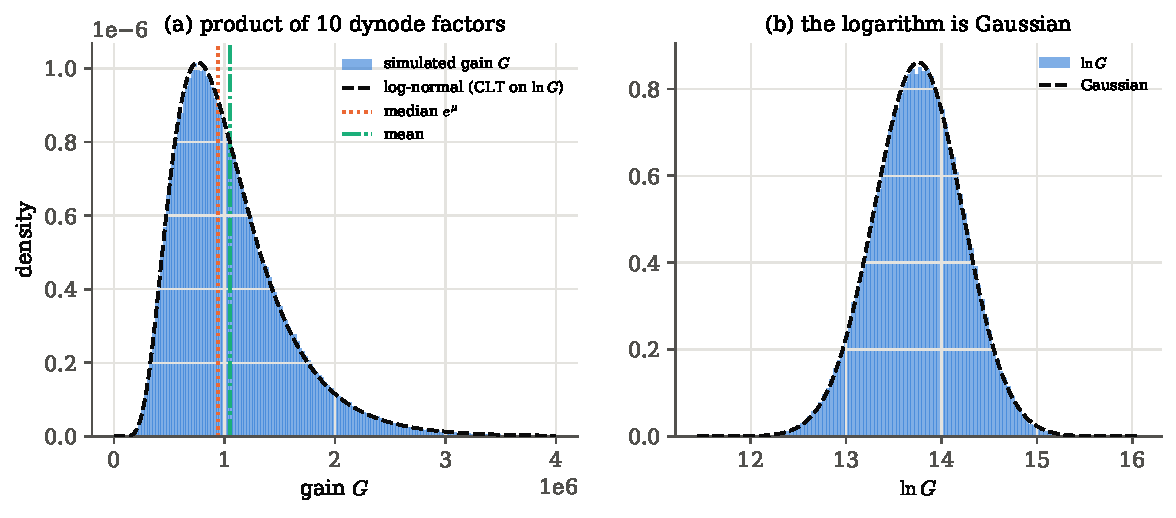
\includegraphics[width=\linewidth]{figures/ch02/zoo_lognormal.pdf}
\caption{(a) The simulated gain of a ten-stage photomultiplier (histogram) and the log-normal predicted by applying the central limit theorem to $\ln G$ (dashed). The median $e^\mu$ (dotted) lies well below the mean (dash-dotted). (b) The same gains on a logarithmic axis: a symmetric Gaussian.}
\label{2b:fig:lognormal}
\end{figure}

\begin{pitfall}[Averaging logarithms gives the median, not the mean]
For a log-normal quantity, $\exp(\overline{\ln x})$ estimates the median $e^\mu$, which is smaller than the mean by the factor $e^{\sigma^2/2}$ ($11\%$ for the photomultiplier). Fitting a straight line to $\ln x$ and exponentiating the prediction has the same bias. Decide which of the two you need, and correct by $e^{\sigma^2/2}$ if it is the mean.
\end{pitfall}

\subsection{Rayleigh and Maxwell--Boltzmann: the length of a Gaussian vector}
\label{2b:sec:maxwell}

The velocity components $(v_x,v_y,v_z)$ of an argon atom in a gas at temperature $T$ are independent Gaussians with mean zero and variance $s^2=k_BT/m$ (this is the MaxEnt result of \cref{2b:sec:maxent-family}, or the Boltzmann factor $e^{-mv^2/2k_BT}$). The \emph{speed} $v=|\bm v|$ is the length of a three-dimensional Gaussian vector. We derived its distribution in all but name in the geometric route to $\chi^2$: the density of $\bm v$ is $(2\pi s^2)^{-3/2}e^{-v^2/2s^2}$, and the volume of the shell at radius $v$ is $S_2v^2\dd v=4\pi v^2\dd v$. Hence
\begin{equation}
  f(v)\eqby{1}4\pi v^2\,\frac{e^{-v^2/2s^2}}{(2\pi s^2)^{3/2}}\eqby{2}\sqrt{\frac2\pi}\;\frac{v^2}{s^3}\;e^{-v^2/2s^2},\qquad v>0 ,
  \label{2b:eq:maxwell}
\end{equation}
\begin{explain}
  \item The shell argument of \eqref{2b:eq:sphere-area} with $\nu=3$.
  \item $4\pi/(2\pi)^{3/2}=\sqrt{2/\pi}$.
\end{explain}
This is the Maxwell--Boltzmann speed distribution. Equivalently, $v^2/s^2\sim\chi^2_3$. Its three landmark speeds, the most probable, the rms and the mean, are
\begin{align}
  v_{\mathrm{mode}}&\eqby{1}\sqrt2\,s=\sqrt{\frac{2k_BT}{m}},\qquad
  v_{\mathrm{rms}}\eqby{2}\sqrt3\,s , \nonumber\\
  \E v&\eqby{3}\sqrt{\frac2\pi}\,\frac{1}{s^3}\int_0^\infty v^3e^{-v^2/2s^2}\dd v\eqby{4}\sqrt{\frac8\pi}\,s=\sqrt{\frac{8k_BT}{\pi m}} .
  \label{2b:eq:maxwell-moments}
\end{align}
\begin{explain}
  \item $\frac{\dd}{\dd v}\bigl(v^2e^{-v^2/2s^2}\bigr)=\bigl(2v-v^3/s^2\bigr)e^{-v^2/2s^2}=0$ at $v^2=2s^2$.
  \item $\E v^2=s^2\,\E\chi^2_3=3s^2$: equipartition, $\frac12m\E v^2=\frac32k_BT$.
  \item Definition of the mean.
  \item With $t=v^2/2s^2$, $\int_0^\infty v^3e^{-v^2/2s^2}\dd v=2s^4\int_0^\infty te^{-t}\dd t=2s^4$, and $\sqrt{2/\pi}\cdot2s=\sqrt{8/\pi}\,s$.
\end{explain}
For argon at $300$\,K the script finds $s=\tbMBsv$\,m/s, and from $4\times10^5$ simulated atoms a mean speed of $\tbMBmean$\,m/s (theory $\tbMBmeanTh$), with the mode at $\tbMBmodeTh$ and the rms speed at $\tbMBrms$ (theory $\tbMBrmsTh$) (\cref{2b:fig:rayleigh}b).

In two dimensions the shell has circumference $2\pi r$, and the same argument gives the \newterm{Rayleigh} distribution
\begin{equation}
  f(r)=\frac{r}{s^2}\,e^{-r^2/2s^2},\qquad \E r=s\sqrt{\pi/2},\qquad r^2\sim s^2\chi^2_2 ,
  \label{2b:eq:rayleigh}
\end{equation}
and the squared length $r^2$ is \emph{exponential} with mean $2s^2$, since $\chi^2_2=$ Gamma$(1,2)$. Of all the cases in this book, this one reaches furthest. A complex Gaussian mode $z=x+iy$, with independent real and imaginary parts of equal variance, has a Rayleigh amplitude $|z|$, a uniform phase, and an exponential power $|z|^2$. That describes a Fourier mode $\tilde\delta(\bm k)$ of a Gaussian random field (\cref{ch:07}), each $\alm$ with $m\neq0$ on the CMB sky, and each frequency bin of Gaussian detector noise in a gravitational-wave periodogram.

\emph{What follows for the scatter of a measured power?} The exponential has standard deviation equal to its mean. So a raw periodogram fluctuates by $100\%$ in every bin, however long the data stream. Only averaging reduces the scatter: over bins or segments (Welch's method), or over the $2\ell+1$ values of $m$, which gives the cosmic variance of \cref{2b:sec:chi2-many}. The script checks the unit-variance case: $\E|z|=\tbRAYmean$ against $\sqrt{\pi/2}=\tbRAYmeanTh$, and $|z|^2$ has mean $\tbPOWmean$ and standard deviation $\tbPOWsd$, both $2$ for an exponential (\cref{2b:fig:rayleigh}a).

\begin{figure}[htbp]
\centering
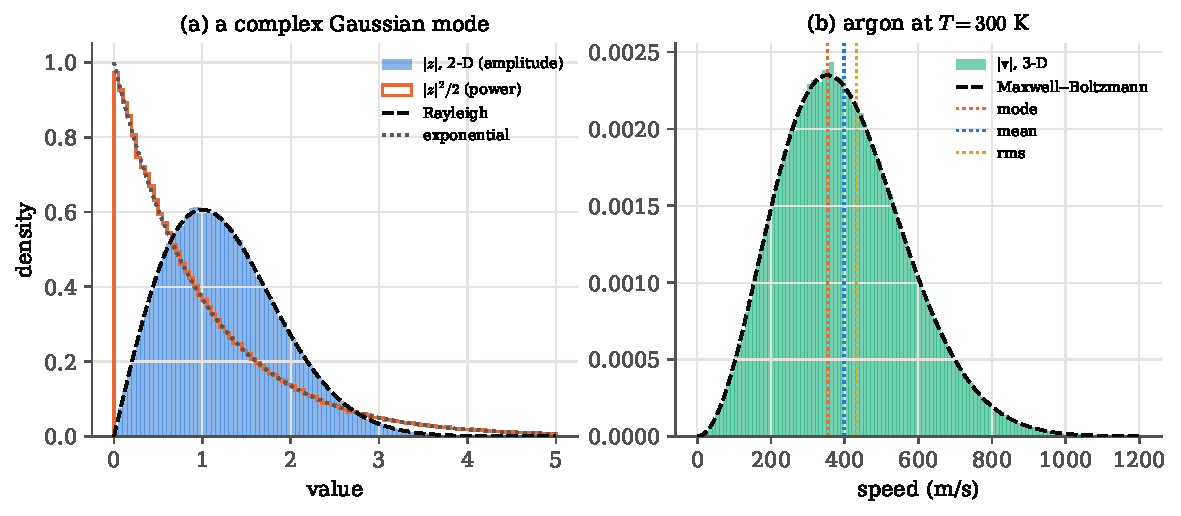
\includegraphics[width=\linewidth]{figures/ch02/zoo_rayleigh_maxwell.pdf}
\caption{(a) The amplitude of a complex Gaussian mode follows the Rayleigh density, and half its squared amplitude, the power, follows a unit exponential. (b) Speeds of simulated argon atoms at $300$\,K against the Maxwell--Boltzmann law, with the mode, the mean and the rms speed marked in that order.}
\label{2b:fig:rayleigh}
\end{figure}

\subsection{Beta: probabilities of probabilities}
\label{2b:sec:beta}

The distributions so far describe data. The beta distribution usually describes a \emph{probability}: the efficiency of a trigger, the bias of a coin, the fraction of events that are signal. It lives on $[0,1]$ and has density \srcref{CasellaBerger}{(3.3.16)}, \srcref{Kruschke}{(6.3)}
\begin{equation}
  f(\theta\given a,b)=\frac{\theta^{a-1}(1-\theta)^{b-1}}{B(a,b)},\qquad
  B(a,b)=\int_0^1\theta^{a-1}(1-\theta)^{b-1}\dd\theta=\frac{\Gamma(a)\Gamma(b)}{\Gamma(a+b)} .
  \label{2b:eq:beta}
\end{equation}
It is produced by three different machines, and each explains something.

\paragraph{Machine 1: sorting uniform numbers.} Draw $n$ independent uniform numbers on $[0,1]$ and let $U_{(k)}$ be the $k$-th smallest, the $k$-th \newterm{order statistic}. For $U_{(k)}$ to lie in $[u,u+\dd u]$, one of the $n$ numbers must fall in that interval, $k-1$ of them below $u$ and $n-k$ above it. The number of ways to choose which is which is the multinomial coefficient $\frac{n!}{(k-1)!\,1!\,(n-k)!}$ of \cref{2a:sec:multinomial}, and the probabilities of the three cells are $u$, $\dd u$ and $1-u$. So
\begin{equation}
  f_{U_{(k)}}(u)\,\dd u=\frac{n!}{(k-1)!\,(n-k)!}\,u^{k-1}(1-u)^{n-k}\,\dd u ,
  \label{2b:eq:orderstat}
\end{equation}
which is Beta$(k,n-k+1)$, with $B(k,n-k+1)=\frac{(k-1)!(n-k)!}{n!}$ \srcref{CasellaBerger}{Ex.~5.4.5}. For a general continuous parent with cumulative distribution $F$ and density $f$, the same count gives $\frac{n!}{(k-1)!(n-k)!}F(x)^{k-1}[1-F(x)]^{n-k}f(x)$ \srcref{CasellaBerger}{Thm~5.4.4}. Casella and Berger prove it by differentiating the binomial probability that at least $k$ of the $n$ values lie below $x$. The same counting gives the joint density of two order statistics, and from it the distribution of the range $U_{(n)}-U_{(1)}\sim$ Beta$(n-1,2)$ \srcref{CasellaBerger}{Thm~5.4.6, Ex.~5.4.7}. 

Order statistics describe the median, quantiles, the fastest of $n$ photon arrival times (which sets the timing of a scintillator), and the largest of $n$ noise fluctuations (the look-elsewhere effect of \cref{ch:04}). With $n=\tbOSn$ and $k=\tbOSk$ the script finds the mean and variance of $U_{(3)}$ to be $\tbOSmean$ and $\tbOSvar$, against $\frac{k}{n+1}=\tbOSmeanTh$ and $\frac{k(n-k+1)}{(n+1)^2(n+2)}=\tbOSvarTh$ (\cref{2b:fig:beta-origins}a).

\paragraph{Machine 2: the share of a total.} Let $X\sim$ Gamma$(a,1)$ and $Y\sim$ Gamma$(b,1)$ be independent. They could be the waiting times for the $a$-th and the $b$-th events of two independent unit-rate processes, or two $\chi^2$ variables. What is the distribution of the share $U=X/(X+Y)$? Change variables to $S=X+Y$ and $U$, so $X=SU$, $Y=S(1-U)$, with Jacobian $\bigl|\partial(x,y)/\partial(s,u)\bigr|=s$:
\begin{align}
  f(u,s)
  &\eqby{1}s\;\frac{(su)^{a-1}e^{-su}}{\Gamma(a)}\;\frac{(s(1-u))^{b-1}e^{-s(1-u)}}{\Gamma(b)} \nonumber\\
  &\eqby{2}\underbrace{\frac{\Gamma(a+b)}{\Gamma(a)\Gamma(b)}\,u^{a-1}(1-u)^{b-1}}_{\text{Beta}(a,b)}\;\times\;\underbrace{\frac{s^{a+b-1}e^{-s}}{\Gamma(a+b)}}_{\text{Gamma}(a+b,1)} .
  \label{2b:eq:gamma-ratio}
\end{align}
\begin{explain}
  \item The joint density of independent $X$ and $Y$ at $x=su$, $y=s(1-u)$, times the Jacobian. The determinant of $\begin{pmatrix}u&s\\1-u&-s\end{pmatrix}$ is $-us-s(1-u)=-s$.
  \item Collect powers: $s\cdot s^{a-1}s^{b-1}=s^{a+b-1}$, and $e^{-su}e^{-s(1-u)}=e^{-s}$. Multiply and divide by $\Gamma(a+b)$.
\end{explain}
The density factorises, so the share $U$ is Beta$(a,b)$ and is \emph{independent} of the total $S$. As a by-product, the second factor integrates to one, so the first must too, which proves $B(a,b)=\Gamma(a)\Gamma(b)/\Gamma(a+b)$ \srcref{CasellaBerger}{(3.3.17)}. With $a=2.5$, $b=4$ the script finds $\E U=\tbGRmean$ against $a/(a+b)=\tbGRmeanTh$ (\cref{2b:fig:beta-origins}b). The relation of $F$ to the beta distribution in \cref{2b:sec:F} is this machine applied to two $\chi^2$ variables.

\paragraph{Summary numbers and shapes.} Recognising kernels again, $\E\theta^r=B(a+r,b)/B(a,b)$ \srcref{CasellaBerger}{(3.3.18)}, so
\begin{equation}
  \E\theta=\frac{a}{a+b},\qquad \Var\theta=\frac{ab}{(a+b)^2(a+b+1)},\qquad \text{mode}=\frac{a-1}{a+b-2}\ \ (a,b>1).
  \label{2b:eq:beta-moments}
\end{equation}
The two shape parameters make the family flexible (\cref{2b:fig:beta-shapes}). It is uniform for $a=b=1$, U-shaped for $a,b<1$, J-shaped when one of them is below one, and single-peaked for $a,b>1$. It is symmetric when $a=b$, with variance $1/[4(2a+1)]$.

\emph{How do we choose $a$ and $b$?} Kruschke's advice \srcref{Kruschke}{p.~128--131} is to think of $a$ and $b$ as ``previously seen'' successes and failures. The concentration $\kappa=a+b$ measures how much prior data that is, and
\[
  a=\mu\kappa,\quad b=(1-\mu)\kappa\qquad\text{or}\qquad a=\omega(\kappa-2)+1,\quad b=(1-\omega)(\kappa-2)+1
\]
set the mean $\mu$ or the mode $\omega$ \srcref{Kruschke}{(6.5)--(6.6)}. A prior with mode $0.8$ and concentration $12$ is Beta$(9,3)$. From a desired mean and standard deviation, $a=\mu\nu$ and $b=(1-\mu)\nu$ with $\nu=\mu(1-\mu)/\sigma^2-1$ \srcref{Kruschke}{(6.7)}: mean $0.5$ and standard deviation $0.1$ give Beta$(12,12)$. The standard deviation must be below $1/\sqrt{12}=0.289$, that of the uniform, or the formula returns a U-shaped (or impossible) answer.

\begin{figure}[htbp]
\centering
\begin{tikzpicture}
\begin{axis}[width=11cm,height=5.4cm,xmin=0,xmax=1,ymin=0,ymax=4.4,
    xlabel={$\theta$},ylabel={density},
    tick label style={font=\scriptsize},label style={font=\small},
    legend style={font=\scriptsize,at={(0.5,-0.32)},anchor=north,draw=none,fill=none},
    legend columns=2,legend cell align=left]
  \addplot[softgray,thick,domain=0.012:0.988,samples=200] {1/(pi*sqrt(x*(1-x)))};
  \addlegendentry{Beta$(\frac12,\frac12)$: U-shaped}
  \addplot[black,thick,dashed,domain=0:1,samples=2] {1};
  \addlegendentry{Beta$(1,1)$: uniform}
  \addplot[fibreorange,thick,domain=0:1,samples=200] {30*x*(1-x)^4};
  \addlegendentry{Beta$(2,5)$}
  \addplot[formblue,thick,domain=0:1,samples=200] {495*x^8*(1-x)^2};
  \addlegendentry{Beta$(9,3)$: mode $0.8$, $\kappa=12$}
  \addplot[tangentgreen,thick,domain=0:1,samples=200] {16224936*x^11*(1-x)^11};
  \addlegendentry{Beta$(12,12)$: mean $0.5$, sd $0.1$}
\end{axis}
\end{tikzpicture}
\caption{Members of the beta family. With both parameters below one the density piles up at the ends; with both equal to one it is flat; above one it has a single peak whose position is set by the ratio of the parameters and whose width shrinks as their sum grows. The blue and green curves are Kruschke's two worked prior specifications.}
\label{2b:fig:beta-shapes}
\end{figure}

\begin{workdef}[beta distribution]
$\theta\sim$ Beta$(a,b)$, $a,b>0$, has density \eqref{2b:eq:beta} on $[0,1]$ and moments \eqref{2b:eq:beta-moments}.
\emph{Recognise it by:} a probability or a fraction that is itself uncertain. It is the $k$-th smallest of $n$ uniform numbers (Beta$(k,n-k+1)$), the share $X/(X+Y)$ of two independent gamma variables with a common scale (Beta$(a,b)$), and, as shown next, the updated belief about a success probability after $a-1$ successes and $b-1$ failures observed from a flat start \unpack{with prior Beta$(a_0,b_0)$ and $h$ successes in $N$ trials the result is Beta$(a_0+h,b_0+N-h)$}.
\end{workdef}

\paragraph{Machine 3: keep the runs that match.} The third machine is inference itself. A coin has unknown bias $\theta$. Before flipping it, our belief about $\theta$ is Beta$(2,2)$: probably near a half, but anything is possible. \emph{The event.} We flip it $N=10$ times and see $h=7$ heads. \emph{The question.} Which values of $\theta$ could have produced seven heads, and how strongly should we now believe in each? Let the computer answer by brute force, with no formula at all. Draw $\theta$ from the prior; flip a coin with that $\theta$ ten times; keep $\theta$ if and only if the run produced exactly seven heads; repeat.

\pyfile[firstline=44,lastline=50,firstnumber=44]{code/ch02/28_beta_dirichlet.py}{Keep the runs that match: a posterior by rejection}

Line 46 draws two million values of $\theta$ from the prior. Line 47 runs the \emph{forward} model, the prediction direction of \cref{ch:01}: for each $\theta$, simulate the experiment. Line 48 keeps only those $\theta$ that reproduced the data, which is conditioning on the observation, the inference direction. The histogram of the kept values is the answer (\cref{2b:fig:beta-origins}c). \emph{What is it analytically?} Take the candidate values of $\theta$ one at a time. A given $\theta$ is kept with the binomial probability of the data, $\binom{10}{7}\theta^7(1-\theta)^3$. It was drawn in the first place with the prior density. So the kept values have density proportional to the product of the two,
\[
  \underbrace{\theta(1-\theta)}_{\text{Beta}(2,2)\text{ kernel}}\times\underbrace{\theta^7(1-\theta)^3}_{\text{probability of the data}}=\theta^{8}(1-\theta)^{4},
\]
the kernel of Beta$(9,5)$. In general, prior Beta$(a_0,b_0)$ and binomial data give Beta$(a_0+h,b_0+N-h)$. The family is \newterm{conjugate} to the binomial: prior and posterior belong to the same family. And ``$a$ and $b$ are previous successes and failures'' is literally true. The script's kept values have mean $\tbRJmean$ and standard deviation $\tbRJsd$, against $\frac{9}{14}=\tbRJmeanTh$ and $\tbRJsdTh$.

The acceptance fraction has a meaning too. It is $\tbRJacc$, the probability of seeing seven heads averaged over the prior, $\binom{10}{7}B(9,5)/B(2,2)=\tbRJaccTh$. That is the \emph{evidence}, the denominator of Bayes' theorem. So this little machine is the whole of \cref{ch:05} in miniature. Rejection wastes $89\%$ of the draws here. It would waste nearly all of them for a continuous observation or many parameters, which is why \cref{ch:09} replaces it by Markov chain Monte Carlo. The same logic makes the gamma distribution conjugate to the Poisson rate: a Gamma$(\alpha,\beta)$ prior times the Poisson likelihood $\lambda^ne^{-\lambda}$ is again a gamma kernel.

\begin{figure}[htbp]
\centering
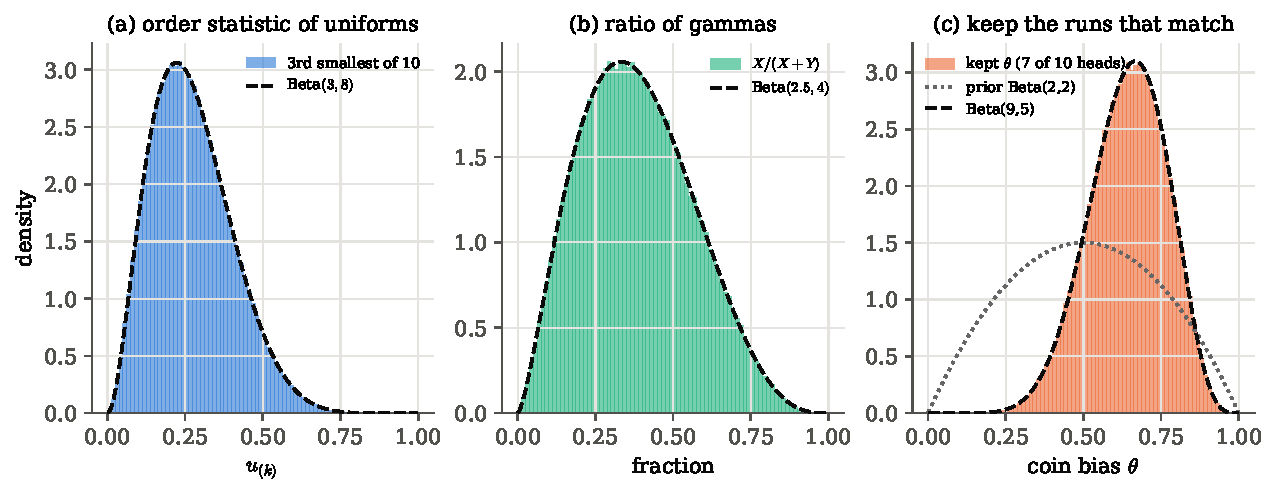
\includegraphics[width=\linewidth]{figures/ch02/beta_origins.pdf}
\caption{Three machines that make a beta distribution. (a) The third smallest of ten uniform numbers. (b) The share $X/(X+Y)$ of two independent gamma variables. (c) Coin biases drawn from a Beta$(2,2)$ prior (dotted) and kept only when their simulated ten flips gave seven heads: the survivors follow Beta$(9,5)$.}
\label{2b:fig:beta-origins}
\end{figure}

\subsection{Dirichlet: several probabilities that sum to one}
\label{2b:sec:dirichlet}

A histogram with $K$ bins has bin probabilities $p_1,\dots,p_K$ with $\sum_jp_j=1$; an election has vote shares; a decay has branching ratios. The distribution for such a vector is the \newterm{Dirichlet}, and the gamma machine of \eqref{2b:eq:gamma-ratio} (Machine~2, the share of a total) builds it. Draw independent $G_j\sim$ Gamma$(\alpha_j,1)$, $j=1,\dots,K$, and normalise, $p_j=G_j/\sum_lG_l$. The same change of variables, now with $K$ variables, gives the density on the simplex \unpack{the set of vectors with all $p_j\ge0$ and $\sum_jp_j=1$, a triangle for $K=3$}
\begin{equation}
  f(p_1,\dots,p_K)=\frac{\Gamma(\alpha_0)}{\prod_j\Gamma(\alpha_j)}\prod_{j=1}^Kp_j^{\alpha_j-1},\qquad \alpha_0=\sum_j\alpha_j ,
  \label{2b:eq:dirichlet}
\end{equation}
which reduces to the beta for $K=2$. Its properties follow from the machine without any integration. \emph{Marginals.} One component is $p_1=G_1/(G_1+R)$ with $R=\sum_{j\ge2}G_j\sim$ Gamma$(\alpha_0-\alpha_1,1)$ by \eqref{2b:eq:gamma-add}, so by machine 2 each marginal is a beta,
\[
  p_j\sim\text{Beta}(\alpha_j,\alpha_0-\alpha_j),\qquad \E p_j=\frac{\alpha_j}{\alpha_0},\qquad \Var p_j=\frac{\alpha_j(\alpha_0-\alpha_j)}{\alpha_0^2(\alpha_0+1)} .
\]
\emph{Covariances.} These follow from the constraint $\sum_jp_j=1$. For $K=3$, $p_1+p_2=1-p_3$, so
\begin{align}
  2\Cov(p_1,p_2)
  &\eqby{1}\Var p_3-\Var p_1-\Var p_2 \nonumber\\
  &\eqby{2}\frac{\alpha_3(\alpha_0-\alpha_3)-\alpha_1(\alpha_0-\alpha_1)-\alpha_2(\alpha_0-\alpha_2)}{\alpha_0^2(\alpha_0+1)}
   \eqby{3}\frac{-2\alpha_1\alpha_2}{\alpha_0^2(\alpha_0+1)} .
  \label{2b:eq:dirichlet-cov}
\end{align}
\begin{explain}
  \item $\Var(p_1+p_2)=\Var(1-p_3)=\Var p_3$, and $\Var(p_1+p_2)=\Var p_1+\Var p_2+2\Cov(p_1,p_2)$.
  \item Insert the beta variances.
  \item Write $s=\alpha_1+\alpha_2$, so $\alpha_3=\alpha_0-s$. The numerator is $(\alpha_0-s)s-\alpha_1(\alpha_0-\alpha_1)-\alpha_2(\alpha_0-\alpha_2)=-s^2+\alpha_1^2+\alpha_2^2=-2\alpha_1\alpha_2$.
\end{explain}
So $\Cov(p_i,p_j)=-\alpha_i\alpha_j/[\alpha_0^2(\alpha_0+1)]$ for $i\neq j$ (for $K>3$ lump the other components into one, which is again gamma), the same negative-correlation pattern as the multinomial counts of \eqref{2a:eq:multcov}: if one share grows, the others must shrink.

For Lambert's three-party election with Dirichlet$(4,2,2)$ \srcref{Lambert}{\S8.5.1}, the script finds $\E p_1=\tbDIRmeanOne$ ($\tbDIRmeanOneTh$), $\Var p_1=\tbDIRvarOne$ ($\tbDIRvarOneTh$) and $\Cov(p_1,p_2)=\tbDIRcov$ ($\tbDIRcovTh$) (\cref{2b:fig:dirichlet}). Two facts decide when to use it. It is conjugate to the multinomial, exactly as the beta is to the binomial: prior Dirichlet$(\bm\alpha)$ and bin counts $\bm n$ give Dirichlet$(\bm\alpha+\bm n)$. And, as Lambert warns, its correlations are all fixed by the $\alpha$'s, so it cannot express a belief such as ``if party 2 does well, so does party 3''; logistic-normal priors are used when that matters.

\begin{figure}[htbp]
\centering
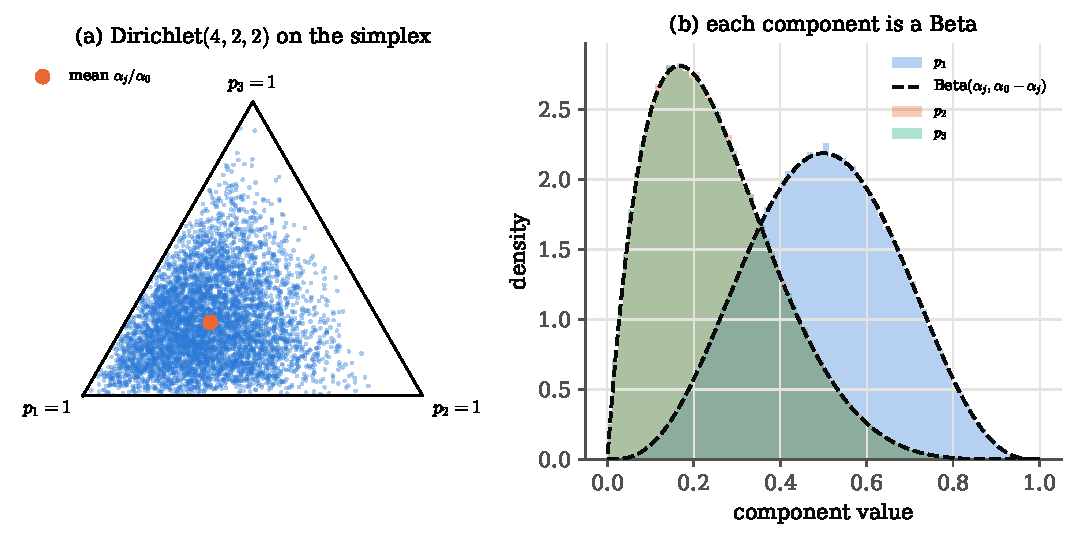
\includegraphics[width=\linewidth]{figures/ch02/dirichlet.pdf}
\caption{(a) Draws from Dirichlet$(4,2,2)$ on the triangle of possible vote shares: each corner is one party winning everything, and the cloud sits nearer the corner of the party with the largest $\alpha$. (b) Each share on its own follows a beta distribution (dashed curves).}
\label{2b:fig:dirichlet}
\end{figure}

\subsection{Two relatives from earlier sections}
\label{2b:sec:relatives}

Two more distributions complete the zoo, and both have appeared already. The \newterm{Laplace} or double-exponential density $\frac{1}{2\sigma}e^{-|x-\mu|/\sigma}$, with $\Var=2\sigma^2$ \srcref{CasellaBerger}{(3.3.22)--(3.3.23)}, was the MaxEnt answer for a known mean absolute deviation. Its machine is the difference of two independent exponential waits with the same mean $\sigma$. To check, multiply the characteristic functions: $(1-i\sigma k)^{-1}(1+i\sigma k)^{-1}=(1+\sigma^2k^2)^{-1}$, which is the transform of the Laplace density. It has a cusp at the centre and exponential tails, fatter than Gaussian but with all moments finite. The \newterm{Cauchy} (Breit--Wigner) distribution of \cref{2b:sec:cauchy} has three machines: the line shape of an unstable state, the ratio of two independent standard normals \srcref{CasellaBerger}{p.~89}, and Student's $t_1$. Its location parameter is the median, even though it has no mean \srcref{CasellaBerger}{(3.3.19)--(3.3.20)}.

\paragraph{One family tree.} Stepping back, nearly everything in this part hangs from two roots. From the \emph{Gaussian}: squares give $\chi^2$, lengths give Rayleigh and Maxwell, ratios give $t$, $F$ and Cauchy, exponentials give the log-normal, linear maps give the multivariate normal. From the \emph{exponential} (the waiting time of a Poisson process): sums give the gamma, shares of sums give the beta and the Dirichlet, powers give the Weibull, differences give the Laplace. The two trees meet at $\chi^2_\nu=$ Gamma$(\nu/2,2)$, and $\chi^2_2$ is itself an exponential. \Cref{2b:sec:which} collects them into one table.
\section{Which distribution when}
\label{2b:sec:which}

A new set of numbers arrives: the invariant masses of a few thousand dielectron events, the output of a matched filter running over a month of detector noise, the $\chi^2$ of a fit that took a week to set up. Someone asks what distribution the numbers follow. The tempting answer is to make a histogram and pick whichever curve from the zoo looks closest. The better order is the opposite one. Every distribution of this chapter came out of a machine, and the machine is what we can know before seeing a single number. So the question ``which distribution?'' becomes ``which machine made these numbers?''. The histogram comes afterwards, to check the answer where the check is most demanding: in the tails.

Choosing by machine is a procedure, and it can be written down. The machines fit into one family tree and one table. The procedure works on all three kinds of data the book keeps returning to: collider counts, detector noise and fitted spectra. And it has one firm warning attached: two distributions that agree in mean and variance can disagree by factors of thousands where discoveries are claimed.

\subsection{Reading the mechanism}
\label{2b:sec:which-procedure}

Before fitting any curve, we answer four questions about how the number was made.
\begin{enumerate}[leftmargin=1.6em,itemsep=1pt]
  \item \emph{Is it a count or a continuous measurement?} Counts go to the counting machines of \cref{2a:sec:bernoulli} to \cref{2a:sec:failures}, whose table ends the previous part. Continuous measurements go to this part.
  \item \emph{Which operation produced it?} Adding many small pieces, multiplying many factors, squaring and adding, taking the length of a vector, dividing one random quantity by another, waiting for an event, taking a share of a total, or sorting.
  \item \emph{Are the ingredients independent, and do they have a finite variance?} If the answer is no, the limit theorems that manufacture Gaussians and $\chi^2$'s are switched off, and a Cauchy or a Landau law (\cref{2b:sec:cauchy,2b:sec:landau}) may be what arrives.
  \item \emph{Which part of the distribution will the conclusion rest on?} An average and its error bar use the centre, where almost any sensible model agrees. A $\pval$-value, a discovery claim or a false-alarm rate uses the tail, where models disagree most.
\end{enumerate}
Lambert draws the same procedure as a decision tree for choosing a likelihood \srcref{Lambert}{\S8.6, Fig.~8.33}, and adds the practical advice to err on the side of robustness \srcref{Lambert}{\S8.8}: when unsure, prefer the model with heavier tails (the negative binomial over the Poisson, Student's $t$ over the Gaussian).

Most continuous distributions descend from just two parents, the Gaussian and the exponential. \Cref{2b:fig:family} arranges the machines as two trees \srcref{Lambert}{\S8.3, Fig.~8.1}. Each box names a distribution and, underneath, the operation that makes it from its parent. The Gaussian tree is the world of sums, the exponential tree the world of waiting. The dashed line is the one place where they are literally the same distribution: $\chi^2_\nu=$ Gamma$(\nu/2,2)$, so a sum of $\nu$ squared Gaussians is the wait for the $(\nu/2)$-th event of a Poisson stream of rate $\frac12$. Above both sits the uniform distribution, which by the inverse-transform rule of \cref{2b:sec:uniform} can be turned into any of them.

\begin{figure}[htbp]
\centering
\begin{tikzpicture}[x=0.9cm,y=1cm,
  gbox/.style={draw=formblue,rounded corners=2pt,fill=ideabg,align=center,font=\scriptsize,
               minimum width=1.55cm,minimum height=0.8cm,inner sep=2pt},
  ebox/.style={gbox,draw=fibreorange},
  ubox/.style={gbox,draw=black!55,fill=white},
  garr/.style={->,thick,formblue},
  earr/.style={->,thick,fibreorange},
  uarr/.style={->,thick,black!45}]
  \node[ubox] (U) at (6.6,1.7) {\textbf{uniform} U$(0,1)$\\ $F^{-1}(U)$ gives any law};
  \node[gbox] (G) at (3.2,0) {\textbf{Gaussian}\\ sums (CLT), MaxEnt};
  \node[gbox] (MVN) at (0,-1.8) {\textbf{multivariate}\\ \textbf{normal}\\ linear map};
  \node[gbox] (LN) at (2.15,-1.8) {\textbf{log-normal}\\ exponentiate};
  \node[gbox] (RM) at (4.3,-1.8) {\textbf{Rayleigh},\\ \textbf{Maxwell}\\ length in\\ 2-D, 3-D};
  \node[gbox] (CA) at (6.45,-1.8) {\textbf{Cauchy}\\ ratio of two};
  \node[gbox] (CHI) at (3.2,-3.6) {\textbf{\boldmath$\chi^2_\nu$}\\ sum of $\nu$ squares};
  \node[gbox] (T) at (2.1,-5.4) {\textbf{\boldmath Student $t_\nu$}\\ $Z/\sqrt{\chi^2_\nu/\nu}$\\ ($t_1=$ Cauchy)};
  \node[gbox] (F) at (4.3,-5.4) {\textbf{\boldmath$F_{p,q}$}\\ ratio of two\\ $\chi^2/\text{dof}$};
  \node[ebox] (E) at (10.6,0) {\textbf{exponential}\\ Poisson waits};
  \node[ebox] (GA) at (8.6,-1.8) {\textbf{gamma}\\ sum of waits};
  \node[ebox] (LA) at (10.7,-1.8) {\textbf{Laplace}\\ difference\\ of two};
  \node[ebox] (WE) at (12.8,-1.8) {\textbf{Weibull}\\ power $X^{1/\gamma}$};
  \node[ebox] (BE) at (7.7,-3.6) {\textbf{beta}\\ share $\frac{X}{X+Y}$};
  \node[ebox] (DI) at (9.7,-3.6) {\textbf{Dirichlet}\\ shares of $K$};
  \draw[uarr] (U) -- (G);
  \draw[uarr] (U) -- (E);
  \foreach \c in {MVN,LN,RM,CA,CHI} \draw[garr] (G) -- (\c);
  \draw[garr] (CHI) -- (T);
  \draw[garr] (CHI) -- (F);
  \foreach \c in {GA,LA,WE} \draw[earr] (E) -- (\c);
  \draw[earr] (GA) -- (BE);
  \draw[earr] (GA) -- (DI);
  \draw[tangentgreen,very thick,dashed] (CHI.east) -- (GA.south west);
\end{tikzpicture}
\caption{Two family trees hold most of the continuous zoo. Blue: everything built from Gaussians, with the building operation written under each name. Orange: everything built from the exponential waiting time of a Poisson process. The green dashed line joins $\chi^2_\nu$ and the gamma family, which are the same distribution. The uniform at the top feeds both trees, since any law is $F^{-1}$ of a uniform number.}
\label{2b:fig:family}
\end{figure}

The table collects the continuous machines with their summary numbers and the places they turn up in physics. Every mean and variance in it was derived earlier in the chapter, and the section that derived it also gives the density.

\begin{taxonomy}[which continuous distribution, when]
\centering\footnotesize
\renewcommand{\arraystretch}{1.22}
\begin{tabularx}{\linewidth}{@{}>{\raggedright\arraybackslash}p{3.55cm}>{\raggedright\arraybackslash}p{2.05cm}>{\raggedright\arraybackslash}p{3.0cm}>{\raggedright\arraybackslash}X@{}}
\textbf{mechanism} & \textbf{distribution} & \textbf{mean; variance} & \textbf{physics examples}\\\hline
sum of many small independent pieces with finite variance; or only mean and variance known & $\Normal(\mu,\sigma^2)$ & $\mu$; $\sigma^2$ & measurement and thermal noise, large-$\lambda$ counts, real and imaginary part of a noise Fourier bin\\
linear map $A\bm Z+\bm\mu$ of independent standard normals & $\Normal(\bm\mu,\Cmat)$ & $\bm\mu$; $\Cmat=AA\T$ & correlated parameters, pixels of a Gaussian field, Fisher forecasts\\
only a range known; $F(X)$ of any continuous $X$ & U$(a,b)$ & $\frac{a+b}2$; $\frac{(b-a)^2}{12}$ & strip pitch$/\sqrt{12}$, rounding, random phase, $\pval$-values under $\Hnull$\\
wait for the first event of a constant-rate stream; power of a complex Gaussian mode & Exp$(\lambda)$ & $\frac1\lambda$; $\frac1{\lambda^2}$ & decay times, arrival gaps, periodogram power, $|\alm|^2$\\
sum of $\alpha$ waits; $\chi^2$ with a scale & Gamma$(\alpha,\beta)$ & $\alpha\beta$; $\alpha\beta^2$ & time to the $n$-th photon, prior on a Poisson rate\\
failure rate a power of age & Weibull, $Y=X^{1/\gamma}$, $X\sim$ Exp$(1)$ & $\Gamma(1+\frac1\gamma)$; $\Gamma(1+\frac2\gamma)-\Gamma(1+\frac1\gamma)^2$ & lifetimes of tubes and electronics, extremes\\
product of many positive independent factors & log-normal, $\ln X\sim\Normal(\mu,\sigma^2)$ & $e^{\mu+\sigma^2/2}$; $e^{2\mu+\sigma^2}(e^{\sigma^2}-1)$ & photomultiplier gain, log-normal density-field models\\
sum of $\nu$ squared independent standard normals & $\chi^2_\nu$ & $\nu$; $2\nu$ & goodness of fit, $(n-1)S^2/\sigma^2$, $\Chat$ and cosmic variance\\
length of a 2-D / 3-D Gaussian vector (scale $s$) & Rayleigh / Maxwell & $s\sqrt{\pi/2}$; $(2-\frac\pi2)s^2$ \;/\; $s\sqrt{8/\pi}$; $(3-\frac8\pi)s^2$ & Fourier amplitudes, matched-filter SNR in noise / molecular speeds\\
Gaussian over an independently estimated scale & Student $t_\nu$ & $0$ ($\nu>1$); $\frac{\nu}{\nu-2}$ ($\nu>2$) & mean with an estimated error bar, likelihood robust to outliers\\
ratio of two independent $\chi^2/\text{dof}$ & $F_{p,q}$ & $\frac{q}{q-2}$ ($q>2$) & comparing two resolutions, nested fits\\
resonance line shape; ratio of two normals & Cauchy (Breit--Wigner) & none; none (median $M$, half-width $\gamma$) & unstable-particle mass, natural line width\\
resonance seen with Gaussian resolution & Voigt & none; none & measured mass peaks, pressure-broadened lines\\
energy lost in a thin layer & Landau & none; none & $\dd E/\dd x$ in silicon and gas\\
uncertain probability; $k$-th of $n$ uniforms; share of two gammas & Beta$(a,b)$ & $\frac{a}{a+b}$; $\frac{ab}{(a+b)^2(a+b+1)}$ & efficiencies, branching fractions, prior on a success probability\\
uncertain probability vector & Dirichlet$(\bm\alpha)$ & $\frac{\alpha_j}{\alpha_0}$; $\frac{\alpha_j(\alpha_0-\alpha_j)}{\alpha_0^2(\alpha_0+1)}$ & bin probabilities of a histogram, branching ratios\\
difference of two equal exponentials; known mean absolute deviation & Laplace$(\mu,\sigma)$ & $\mu$; $2\sigma^2$ & least-absolute-deviation fits\\
\end{tabularx}
\end{taxonomy}

One row of the table is new, the Voigt profile. It is the first of three recognition problems, and it shows how two rows combine.

\subsection{Three recognitions}
\label{2b:sec:which-examples}

\paragraph{Example: a Z peak seen through a detector.} In \cref{2b:sec:cauchy} the Z line shape was the Breit--Wigner \eqref{2b:eq:bw}, with detector resolution ignored. A real calorimeter adds to each true mass $B$ an independent Gaussian error $G\sim\Normal(0,\sigma^2)$, with $\sigma=\tbWsig$\,GeV for our example. The measured mass is $m=B+G$. \emph{The question:} does the smearing turn the peak into a Gaussian, and what happens to the tails? \emph{Reading the mechanism:} a \emph{sum} of two independent pieces, so the characteristic function is a product:
\begin{align}
  \phi_m(k)
  &\eqby{1}\E\bigl(e^{ikB}\bigr)\,\E\bigl(e^{ikG}\bigr)
   \eqby{2}e^{iMk-\gamma|k|}\;e^{-\sigma^2k^2/2},\qquad \gamma=\Gamma/2 .
  \label{2b:eq:voigt-cf}
\end{align}
\begin{explain}
  \item $e^{ik(B+G)}=e^{ikB}e^{ikG}$, and the expectation of a product of independent factors is the product of expectations, \eqref{2b:eq:cf-sum}.
  \item The Cauchy transform \eqref{2b:eq:cf-cauchy} with centre $M$ and half-width $\gamma$, and the Gaussian transform \eqref{2b:eq:cf-gauss} with mean zero.
\end{explain}
The inverse transform of \eqref{2b:eq:voigt-cf} is the \newterm{Voigt profile}, the convolution of the two densities. It has no closed form, but the characteristic function already answers the question: no, the Cauchy tail survives. First, $\phi_m$ still has the kink $|k|$ at $k=0$, so it is not differentiable there and $m$ still has no mean: Gaussian smearing cannot cure a Cauchy tail. Second, the tail itself survives unchanged. For $|m-M|$ much larger than both $\sigma$ and $\gamma$,
\begin{align}
  p_m(m)
  &\eqby{1}\int_{-\infty}^{\infty}p_B(m-g)\,p_G(g)\,\dd g
   \eqby{2}p_B(m)\int_{-\infty}^{\infty}p_G(g)\,\dd g\,\bigl[1+O(\sigma^2/(m-M)^2)\bigr] \nonumber\\
  &\eqby{3}\frac1\pi\,\frac{\gamma}{(m-M)^2+\gamma^2}\,\bigl[1+\dots\bigr]
   \eqby{4}\frac{\gamma}{\pi\,(m-M)^2}\,\bigl[1+\dots\bigr] .
  \label{2b:eq:voigt-tail}
\end{align}
\begin{explain}
  \item The density of a sum of independent variables is the convolution of their densities: to reach $m$, the Gaussian must supply $g$ and the resonance $m-g$.
  \item $p_G$ is non-negligible only for $|g|\lesssim3\sigma$, and over that range the Breit--Wigner, far out in its tail, changes little. Expanding $p_B(m-g)$ to second order in $g$, the linear term averages to zero because $\E G=0$, and the quadratic term is smaller by a factor of order $\sigma^2/(m-M)^2$.
  \item $p_G$ integrates to one, and \eqref{2b:eq:bw} written with $\gamma=\Gamma/2$.
  \item $(m-M)^2\gg\gamma^2$.
\end{explain}
So the fraction of events more than $\Delta$ from the peak is, for $\Delta\gg\sigma,\gamma$,
\begin{align}
  \Prob(|m-M|>\Delta)
  \eqby{1}2\int_\Delta^\infty\frac{\gamma}{\pi u^2}\,\dd u
  \eqby{2}\frac{2\gamma}{\pi\Delta} ,
  \label{2b:eq:voigt-frac}
\end{align}
\begin{explain}
  \item The symmetry of the two tails and the approximation \eqref{2b:eq:voigt-tail} with $u=|m-M|$.
  \item $\int_\Delta^\infty u^{-2}\dd u=1/\Delta$.
\end{explain}
For $\gamma=1.2476$\,GeV and $\Delta=\tbWDelta$\,GeV this gives $\tbWoutTail$.

\pyfile[firstline=37,lastline=51,firstnumber=37]{code/ch02/29_which_distribution.py}{A Breit--Wigner resonance smeared by Gaussian resolution}

The script builds the machine literally, and the Gaussian fails by a factor of several hundred in the wings. Line 39 adds a Cauchy draw of half-width $\gamma$ and a Gaussian draw of width $\sigma$ to the Z mass, for each of $2\times10^5$ events. Line 41 counts the fraction of events beyond $\Delta$. Lines 42--44 integrate the exact Voigt density (\pyname{scipy.special.voigt_profile}, whose arguments are the Gaussian $\sigma$ and the Cauchy half-width $\gamma$) over the core. Lines 47--51 find the full width at half maximum of the Voigt profile and build the Gaussian with the same width, the curve one would get by fitting a Gaussian to the peak by eye.

The three estimates of the tail agree: the simulated fraction beyond $\tbWDelta$\,GeV is $\tbWoutSim$, the exact Voigt value is $\tbWoutVoigt$, and the tail estimate \eqref{2b:eq:voigt-frac} is $\tbWoutTail$. The Voigt peak has a full width at half maximum of $\tbWfwhm$\,GeV, and a Gaussian with that width ($\sigma_{\text{eq}}=\tbWsigEq$\,GeV) puts only $\tbWoutGauss$ of its probability beyond $\tbWDelta$\,GeV. On a linear plot the two curves are hard to tell apart. On the logarithmic plot of \cref{2b:fig:which}b the difference is a factor of several hundred. An analysis that modelled the peak as a Gaussian would find about $8\%$ of the Z events in its ``background'' sidebands.

\begin{figure}[htbp]
\centering
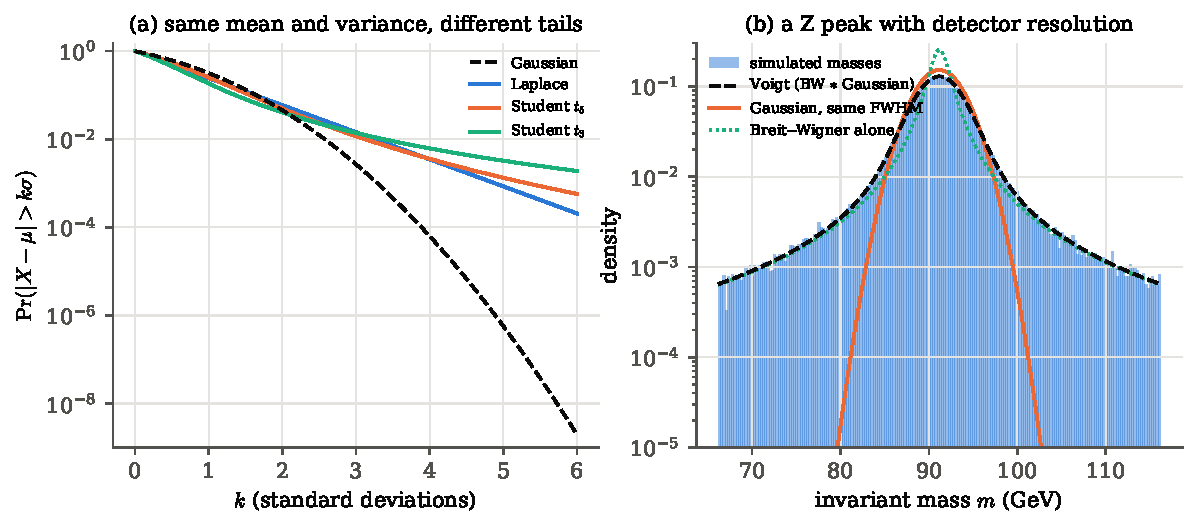
\includegraphics[width=\linewidth]{figures/ch02/which_distribution.pdf}
\caption{(a) Two-sided tail probability against distance from the mean, in units of the standard deviation, for four symmetric distributions scaled to the same mean and variance. They agree within a factor of two out to about two standard deviations and then separate by orders of magnitude. (b) Simulated Z masses with a Breit--Wigner width and Gaussian detector resolution, on a logarithmic scale. The Voigt density (dashed) follows them into the wings; the Gaussian with the same half-maximum width (solid) matches only the core; far from the peak the Voigt rejoins the pure Breit--Wigner (dotted).}
\label{2b:fig:which}
\end{figure}

\paragraph{Example: false alarms in a gravitational-wave search.} A matched filter correlates the detector output with a template waveform whose phase is unknown. It returns two numbers at each time, the correlation with the cosine-phase and with the sine-phase template, normalised so that in pure Gaussian noise each is a standard normal and the two are independent. The signal-to-noise ratio is $\rho=\sqrt{x^2+y^2}$, with $x$ and $y$ the two correlations. \emph{The question:} how often does noise alone push $\rho$ above a threshold? \emph{Reading the mechanism:} \emph{the length of a two-dimensional Gaussian vector}. So $\rho$ is Rayleigh with $s=1$, and $\rho^2$ is $\chi^2_2$, the exponential with mean $2$ (\cref{2b:sec:maxwell}). The chance that noise alone crosses a threshold $\rho_*$ is
\begin{align}
  \Prob(\rho>\rho_*)
  \eqby{1}\Prob(\rho^2>\rho_*^2)
  \eqby{2}\int_{\rho_*^2}^{\infty}\tfrac12e^{-u/2}\,\dd u
  \eqby{3}e^{-\rho_*^2/2} .
  \label{2b:eq:false-alarm}
\end{align}
\begin{explain}
  \item $\rho\ge0$, and squaring is increasing on $[0,\infty)$.
  \item The $\chi^2_\nu$ density \eqref{2b:eq:chi2} with $\nu=2$ is $u^{0}e^{-u/2}/(2\,\Gamma(1))=\frac12e^{-u/2}$.
  \item $\int_a^\infty\frac12e^{-u/2}\dd u=e^{-a/2}$.
\end{explain}
The script checks the formula at $\rho_*=\tbWrstar$: the fraction of $2\times10^5$ noise draws above threshold is $\tbWfaSim$, against $e^{-9/2}=\tbWfaTh$ (script lines 54--59). At the conventional detection threshold $\rho_*=8$ the formula gives $\tbWfaEight$ per independent template and time sample. That looks reassuringly small. But a search examines very many templates at every sample of months of data, so the answer depends on the $\chi^2_2$ law holding fourteen decades down its tail. Real detector noise contains short non-Gaussian bursts (``glitches''), which is exactly the kind of fat tail of \cref{2b:fig:which}a.

So searches do not trust \eqref{2b:eq:false-alarm} for their final significance. They measure the background empirically. They shift one detector's data in time against another's, by more than the light travel time, and count how often noise alone produces a coincident trigger. The formula \emph{verifies} the pipeline on simulated Gaussian noise; the time slides are the research instrument on real data. The same Rayleigh and exponential laws describe the amplitude and the power of a noise frequency bin, which returns in the gravitational-wave Fisher forecasts of \cref{ch:10}, where the noise enters through its power spectral density.

\paragraph{Example: is $\chi^2=130$ for $100$ degrees of freedom a bad fit?} It is suspicious but not damning, and the Gaussian shortcut gets its tail wrong by $40\%$. A fit of a model with $P$ adjustable parameters to $N$ Gaussian measurements returns a minimum $\chi^2$. For a model linear in its parameters, the minimum is a quadratic form in the residuals with $N-P$ independent directions left over (the argument of \cref{2b:sec:chi2-quadform,2b:sec:nminus1}, made precise in \cref{ch:03}). Reading the mechanism: \emph{a sum of $\nu=N-P$ squared standard normals}, so $\chi^2_{\min}\sim\chi^2_\nu$. \emph{The question:} how often would a correct model give $\chi^2\ge130$? With $\nu=100$ it is tempting to use the central limit theorem, since $\chi^2_{100}$ is a sum of $100$ independent $\chi^2_1$ variables, and write $\chi^2\approx\Normal(\nu,2\nu)$:
\[
  z=\frac{\chi^2-\nu}{\sqrt{2\nu}}=\frac{130-100}{\sqrt{200}}=\tbWzGauss ,\qquad \Prob(Z>z)=\tbWpGauss .
\]
The exact tail, from \pyname{scipy.stats.chi2.sf(130, 100)}, is $\tbWpExact$, about $40\%$ larger. \emph{Why?} The parent $\chi^2_1$ is skewed, and the CLT removes skewness only slowly (\cref{2b:sec:clt-rate}). To measure it, we need the cumulants $\kappa_n$ (the Taylor coefficients of $\ln\phi$). The cumulants of $\chi^2_1$ follow from its characteristic function $(1-2ik)^{-1/2}$ \eqref{2b:eq:chi2-cf1}: $\ln\phi=-\frac12\ln(1-2ik)=\sum_{n\ge1}\frac{(2ik)^n}{2n}$, and matching with $\ln\phi=\sum_n\kappa_n(ik)^n/n!$ gives $\kappa_n=2^{n-1}(n-1)!$, so $\kappa_2=2$ and $\kappa_3=8$. Then
\begin{align}
  \gamma_1\bigl(\chi^2_\nu\bigr)
  \eqby{1}\frac{\kappa_3(\chi^2_\nu)}{\kappa_2(\chi^2_\nu)^{3/2}}
  \eqby{2}\frac{\nu\,\kappa_3(\chi^2_1)}{\bigl[\nu\,\kappa_2(\chi^2_1)\bigr]^{3/2}}
  \eqby{3}\frac{8\nu}{(2\nu)^{3/2}}
  =\sqrt{\frac8\nu} .
  \label{2b:eq:chi2-skew}
\end{align}
\begin{explain}
  \item Skewness is the third cumulant in units of the standard deviation cubed, with the cumulants of \eqref{2b:eq:cumulants}.
  \item Cumulants of independent variables add, and $\chi^2_\nu$ is the sum of $\nu$ independent $\chi^2_1$.
  \item $\kappa_3(\chi^2_1)=8$ and $\kappa_2(\chi^2_1)=2$.
\end{explain}
At $\nu=100$ the skewness is still $0.28$. So the right tail is longer than the Gaussian's, and the Gaussian approximation underestimates how often a correct model gives a large $\chi^2$. The verdict itself is mild. A correct model would give $\chi^2\ge130$ in about $2\%$ of repetitions, so the fit is suspicious but not damning, and \cref{ch:04} turns this reasoning into a test. The practical rule is simpler: never use $\Normal(\nu,2\nu)$ for a tail probability when the exact $\chi^2_\nu$ survival function is one line of code.

\subsection{The tails decide}
\label{2b:sec:which-tails}

The three examples share a lesson: the core of each distribution was well described by a Gaussian, and the question was about the tail. \Cref{2b:fig:which}a puts numbers on it. It shows four symmetric distributions, each scaled to mean zero and variance one: the Gaussian, the Laplace, and Student's $t_5$ and $t_3$ (for $t_\nu$ with scale $c$ the variance is $c^2\nu/(\nu-2)$ by \eqref{2b:eq:t-var}, so $c^2=3/5$ and $1/3$). They are indistinguishable at one standard deviation and cross near two. At three standard deviations the two-sided tail probabilities are $\tbWthreeGauss$ for the Gaussian but $\tbWthreeLap$ (Laplace), $\tbWthreeTfive$ ($t_5$) and $\tbWthreeTthree$ ($t_3$), four to five times more. At five standard deviations the Gaussian gives $\tbWfiveGauss$ and $t_3$ gives $\tbWfiveTthree$, a ratio of $\tbWratioTthree$.

\begin{keyidea}[Choose by mechanism, check in the tails]
A distribution is chosen by recognising the machine that made the numbers (sum, product, squares, length, ratio, wait, share). Its mean and variance are then fixed by the machine, but agreement in mean and variance says almost nothing beyond about two standard deviations. Any conclusion that uses a tail probability must justify the tail separately, by the mechanism or by an empirical measurement of the background.
\end{keyidea}

The physics of the tails is usually different from the physics of the core. Cowan makes the point for the two distributions with divergent moments, the Breit--Wigner and the Landau. A real resonance mass is bounded by the masses of its decay products and by the collision energy, and a real energy loss by the energy of the incoming particle, so ``the models break down in the tails of the distributions'' \srcref{Cowan}{pp.~38--39}. Near the peak the idealised machine is accurate; far from it, other mechanisms take over (kinematic limits, radiation, pile-up, detector glitches, non-Gaussian foregrounds).

So particle physicists quote a ``$5\sigma$'' discovery as a tail probability of $2.9\times10^{-7}$ computed from the \emph{distribution of the test statistic}, obtained by simulation or by an asymptotic theorem (\cref{ch:04}), and never from a Gaussian assumption about the data alone. The same caution applies to a posterior interval far from the peak of a posterior (\cref{ch:05}), and to the Fisher forecast of \cref{ch:10}, which is Gaussian by construction and must be checked against a sampled posterior in the tails (\cref{ch:09}).

\begin{pitfall}[A good fit to the peak is not a test of the tails]
A histogram with most of its entries within $\pm2\sigma$ fits a Gaussian, a Laplace or a $t_5$ almost equally well: the $\chi^2$ of the fit is dominated by the populated bins, and the tail bins hold too few entries to discriminate. The choice between them must come from the mechanism, or from a dedicated sample that populates the tails (a control region, a time slide, a large simulation).
\end{pitfall}

With a mechanism in hand, the summary numbers of the table give a first check that costs nothing: compare the sample mean and variance with the predicted ones, the Fano factor for counts (\cref{2a:sec:failures}), and, when enough data exist, the sample skewness with the predicted $\gamma_1$. A mismatch in these moments rules the mechanism out; a match leaves the tails still to be checked.

\begin{recap}[Part summary: continuous distributions]
\begin{itemize}
  \item \textbf{Gaussian, three ways.} (i) The binomial near its peak, by Stirling's formula and a second-order expansion of $\ln p_k$ (de Moivre--Laplace), with error $O(1/n)$ at the peak. (ii) The central limit theorem: the characteristic function of a standardised sum tends to $e^{-k^2/2}$ whenever the parent has finite variance, with error $O(n^{-1/2})$ set by the skewness (Berry--Esseen). (iii) Maximum entropy: the least committal density with a given mean and variance.
  \item \textbf{When the CLT fails or is slow.} Cauchy (Breit--Wigner): no mean, and the average of $n$ draws is as wide as one draw. Landau: finite range in reality, but so skewed that the mean of $25$ layers is still far from Gaussian.
  \item \textbf{Multivariate normal.} $\bm X=\bm\mu+A\bm Z$ with $\Cmat=AA\T$; contours are ellipses, and the region $\Delta\chi^2\le2.30$ (two parameters) holds $68.3\%$; marginals drop rows and columns of $\Cmat$; conditionals shift the mean by $\Cmat_{ba}\Cmat_{aa}^{-1}(\bm x_a-\bm\mu_a)$ and shrink the covariance to the Schur complement.
  \item \textbf{$\chi^2_\nu$.} Sum of $\nu$ squared standard normals, $\chi^2_\nu=$ Gamma$(\nu/2,2)$, mean $\nu$, variance $2\nu$; $(\bm X-\bm\mu)\T\Cmat^{-1}(\bm X-\bm\mu)\sim\chi^2_k$; $(n-1)S^2/\sigma^2\sim\chi^2_{n-1}$, independent of $\bar X$, because estimating the mean uses up one direction.
  \item \textbf{$t$ and $F$.} Student $t_\nu=Z/\sqrt{\chi^2_\nu/\nu}$: the studentised mean, heavier tails, variance $\nu/(\nu-2)$, a scale mixture of Gaussians; $F_{p,q}$ is a ratio of two scaled $\chi^2$ and $t_q^2=F_{1,q}$.
  \item \textbf{The zoo.} Uniform (only a range; parent of all through $F^{-1}$), gamma and Weibull (waits), log-normal (products), Rayleigh and Maxwell (lengths of Gaussian vectors; a complex Gaussian mode has exponential power), beta and Dirichlet (uncertain probabilities, conjugate to binomial and multinomial counts), Laplace (differences of waits).
  \item \textbf{Which one when.} Recognise the mechanism first, then check moments, and check tails separately: laws with equal variance can differ by factors of thousands at $5\sigma$.
\end{itemize}
\end{recap}

\section*{Chapter summary}
\addcontentsline{toc}{section}{Chapter summary}
\label{2b:sec:summary}

Every common probability distribution comes from a machine that generates it. Counting machines give the discrete laws: one trial, many trials, histogram bins, rare events, a random stream in time, the waits between its events, and the ways real detectors break these assumptions. Measuring machines give the continuous laws: the Gaussian three times over, then the multivariate normal, the $\chi^2$, Student's $t$ and the $F$ ratio built from it, and the rest of the continuous zoo built from the Gaussian and the exponential. All of it runs in the direction of \emph{prediction}: fix a hypothesis and ask what data it produces and how often. On the pipeline of \cref{ch:00}, that is the step which says how a statistic $S$ scatters given the parameters $\theta$, $P(S\given\theta)$, for the simplest statistics (counts, sums, sample means and variances, $\chi^2$'s, power-spectrum estimates). Every later chapter either reads such a $P(S\given\theta)$ backwards as a likelihood or builds a new one by simulation. The two tables list each concept, what it means operationally (how to compute, recognise or test it), and where it is used next.

\begin{center}
\small
\renewcommand{\arraystretch}{1.15}
\begin{tabularx}{\linewidth}{@{}>{\raggedright\arraybackslash}p{3.3cm}
                               >{\raggedright\arraybackslash}X
                               >{\raggedright\arraybackslash}p{2.7cm}@{}}
\toprule
\multicolumn{3}{@{}l}{\textbf{Counting distributions (first part)}}\\
concept & operational meaning & used later in\\\midrule
distribution as a mechanism & state the machine and its assumptions, derive the law, then simulate the machine (not the formula) and compare histograms & every chapter\\
Bernoulli & one yes/no trial, $p^x(1-p)^{1-x}$; $N$ trials give $p^z(1-p)^{N-z}$, depending only on the number of successes & \cref{ch:03,ch:05}\\
binomial & successes in $n$ independent trials with the same $p$: count the $\binom nk$ paths; mean $np$, variance $np(1-p)$ & \cref{ch:03,ch:04,ch:05}\\
multinomial & a histogram with a fixed total: binomial marginals, covariance $-Np_ip_j$ between bins & \cref{ch:03,ch:04}\\
Poisson & $n\to\infty$, $np=\lambda$ limit of the binomial; mean $=$ variance $=\lambda$; closed under sums and thinning & \cref{ch:03,ch:04,ch:05,ch:06}\\
Poisson process & constant rate, no memory; $\dd P_n/\dd t=\lambda(P_{n-1}-P_n)$; with a Poisson total, histogram bins become independent Poisson counts & \cref{ch:03,ch:06}\\
exponential, gamma (Erlang) & wait for the first / $n$-th event; memoryless; means $1/\lambda$, $n/\lambda$ & \cref{ch:05,ch:06}\\
geometric, negative binomial & trials to the first / $r$-th success; also a Poisson with gamma-distributed rate (overdispersion) & \cref{ch:03,ch:05}\\
Fano factor & variance over mean of counts; $\approx1$ Poisson, $>1$ fluctuating rate or clumping, $<1$ dead time; judge against $\sqrt{2/(k-1)}$ & \cref{ch:04,ch:08}\\
dead time & recorded rate $n/(1+n\tau)$ or $ne^{-n\tau}$; correcting it removes bias but inflates the variance by $1+n\tau$ & \cref{ch:06}\\
large-count limit & all Poisson cumulants equal $\lambda$, skewness $1/\sqrt\lambda$: Gaussian near the peak, exact Poisson in the tails & \cref{ch:03,ch:04}\\
\bottomrule
\end{tabularx}
\end{center}

\begin{center}
\small
\renewcommand{\arraystretch}{1.15}
\begin{tabularx}{\linewidth}{@{}>{\raggedright\arraybackslash}p{3.3cm}
                               >{\raggedright\arraybackslash}X
                               >{\raggedright\arraybackslash}p{2.7cm}@{}}
\toprule
\multicolumn{3}{@{}l}{\textbf{Continuous distributions (second part)}}\\
concept & operational meaning & used later in\\\midrule
Gaussian $\Normal(\mu,\sigma^2)$ & $\mu$ the centre, $\sigma$ the width; probabilities from $\Phi$; $68.3/95.4/99.7\%$ within $1/2/3\sigma$ & every chapter\\
Stirling, Laplace's method & expand the logarithm of a peaked integrand to second order about its maximum & \cref{ch:05,ch:10}\\
de Moivre--Laplace & binomial near its peak $\approx$ Gaussian with mean $np$, variance $np(1-p)$; error largest in the tails & \cref{ch:03,ch:04}\\
characteristic function & $\E e^{ikX}$, always exists; sums multiply it; cumulants are the Taylor coefficients of its logarithm & \cref{ch:06,ch:07}\\
central limit theorem & standardised sums of finite-variance variables tend to $\Normal(0,1)$; error $\sim\gamma_1/\sqrt n$ (Berry--Esseen); check by simulation & \cref{ch:03,ch:04,ch:06}\\
Cauchy, Landau & no mean: averaging does not narrow a Cauchy; use the median or a truncated mean; Landau sums converge very slowly & \cref{ch:03,ch:06}\\
maximum entropy & least committal distribution given constraints: $p\propto e^{-\sum_j\lambda_jf_j}$; mean $\to$ exponential, variance $\to$ Gaussian & \cref{ch:05}\\
multivariate normal & $\bm\mu+A\bm Z$ with $\Cmat=AA\T$ (Cholesky); ellipses with $\Delta\chi^2=2.30,6.18$ in 2-D; marginal = delete rows and columns; conditional = Schur complement & \cref{ch:07,ch:09,ch:10}\\
$\chi^2_\nu$ & sum of $\nu$ squared standard normals; mean $\nu$, variance $2\nu$; quadratic forms $\bm r\T\Cmat^{-1}\bm r$; exact tail by \pyname{chi2.sf} & \cref{ch:03,ch:04,ch:07,ch:08}\\
sample variance, $n-1$ & $(n-1)S^2/\sigma^2\sim\chi^2_{n-1}$, independent of $\bar X$ for Gaussian data; one direction is used by the mean & \cref{ch:03,ch:04}\\
Student $t$ & mean over an estimated error bar; heavier tails, $t_\nu\to\Normal$ as $\nu\to\infty$; robust likelihood & \cref{ch:04,ch:05}\\
$F$ ratio & ratio of two independent scaled $\chi^2$; compare variances or nested fits; $t^2=F_{1,q}$ & \cref{ch:04}\\
uniform, inverse transform & $F(X)$ is uniform; $F^{-1}(U)$ samples any law; $\pval$-values are uniform under $\Hnull$ & \cref{ch:04,ch:06}\\
log-normal & products of positive factors; mean $e^{\mu+\sigma^2/2}$ above the median $e^\mu$ & \cref{ch:05,ch:07}\\
Rayleigh, Maxwell, exponential power & length of a 2-D / 3-D Gaussian vector; a complex Gaussian mode has Rayleigh amplitude, uniform phase, exponential power & \cref{ch:07,ch:08,ch:10}\\
beta, Dirichlet & uncertain probability (vector); conjugate to binomial (multinomial) counts; ``keep the runs that match'' gives the posterior & \cref{ch:05,ch:09}\\
which distribution when & recognise the mechanism, check the moments, justify the tails separately & \cref{ch:04,ch:10,ch:12}\\
\bottomrule
\end{tabularx}
\end{center}

\subsection*{Reading the literature}

\begin{itemize}[leftmargin=1.2em,itemsep=2pt]
  \item \textbf{Main line.} \mainref{\S\S2.3--2.4, 2.10, 5.4} gives the discrete and continuous families, the multivariate normal with its marginals and conditionals, and the central limit theorem with the Berry--Esseen bound, compactly and with short examples; the MGF proof of the CLT is in \mainref{\S5.7.2}.
  \item \textbf{The clearest first reading.} \srcref{Kruschke}{Ch.~6}: the beta distribution as a description of belief about a probability, its parameters as previous successes and failures, and how to set them from a mean and a spread.
  \item \textbf{The physicist's version.} \srcref{Cowan}{Ch.~2} for each distribution with a physics setting (including the Breit--Wigner and Landau laws and their divergent moments), and \srcref{Cowan}{Ch.~10} for characteristic functions, the limits binomial $\to$ Poisson $\to$ Gaussian, the $\chi^2$ from squares, and the practical validity of the CLT.
  \item \textbf{Careful derivations.} \srcref{CasellaBerger}{\S\S3.2--3.3, 4.5--4.6, 5.3--5.4}: the families with full proofs of their moments, the bivariate and multivariate normal, the independence of $\bar X$ and $S^2$, the $t$ and $F$ densities by Jacobians, and order statistics.
  \item \textbf{Maximum entropy.} \srcref{Sivia}{Ch.~5}: the monkey argument for the entropy, the loaded die, the kangaroo problem, and the exponential, Gaussian, Laplace and Poisson as MaxEnt assignments.
  \item \textbf{Choosing a likelihood and a prior.} \srcref{Lambert}{Ch.~8}: a catalogue of sampling and prior distributions with a story for each, their interrelations, the robust versions (negative binomial, Student $t$), and a decision tree for choosing a likelihood.
  \item \textbf{Pictures.} \srcref{SeeingTheory}{pp.~38--39}: an interactive demonstration of the central limit theorem.
  \item \textbf{Going further.} The Gaussian approximation to the $\Chat$ likelihood and its failure at low $\ell$, where the $\chi^2_{2\ell+1}$ skewness matters, is treated in \cite{HamimecheLewis2008}; \cref{ch:07,ch:08} build on it.
\end{itemize}
  